% !TEX encoding = UTF-8 Unicode
%% GABARIT POUR MÉMOIRE STANDARD
%%
%% Consulter la documentation de la classe ulthese pour une
%% description détaillée de la classe, de ce gabarit et des options
%% disponibles.
%%
%% [Ne pas hésiter à supprimer les commentaires après les avoir lus.]
%%
%% Déclaration de la classe avec le type de grade
%%   [l'un de MATDR, MArch, MA, LLM, MErg, MMus, MPht, MSc, MScGeogr,
%%    MServSoc, MPsEd]
%% et les langues les plus courantes. Le français sera la langue par
%% défaut du document.
\documentclass[MSc,english,french]{ulthese}
  %% Encodage utilisé pour les caractères accentués dans les fichiers
  %% source du document. Les gabarits sont encodés en UTF-8. Inutile
  %% avec XeLaTeX, qui gère Unicode nativement.
  \ifxetex\else \usepackage[utf8]{inputenc} \fi
  %% Charger ici les autres paquetages nécessaires pour le document.
  %% Quelques exemples; décommenter au besoin.
  \usepackage{amsmath}       % recommandé pour les mathématiques
  \usepackage{amssymb}    % using for intercal symbol
  %\usepackage{icomma}        % gestion de la virgule dans les nombres
  \usepackage{mathtools}
  \usepackage{graphicx}
  \usepackage{outlines}  % for nested lists
  \graphicspath{ {./images/} }
  \usepackage{algorithm}
  \usepackage{algpseudocode}
  \usepackage{natbib}   % for citep command
  \usepackage{array}  % for arraybackslash command in tables
  \usepackage{booktabs}  % for table formatting
  \renewcommand{\arraystretch}{1.4}  % Makes table row heights higher

 % \usepackage{easyReview}  % Only used for highlighting edits - REMOVE IN FINAL DRAFT

% This package raises warnings 'overriding \printglossary'. 'overriding 'theglossary' environment
\usepackage[acronym]{glossaries}
\makeglossaries
% According to this, these warnings can be ignored:
% https://tex.stackexchange.com/questions/163479/glossaries-conflict-with-memoir

% General notation
\newglossaryentry{qm1}{name=$q^{-1}$, description={backwards shift operator}}
\newglossaryentry{pk}{name=$p(k)$, description={disturbance signal at time $k$}}
\newglossaryentry{wpk}{name=$w_p(k)$, description={random shock signal at time $k$}}
\newglossaryentry{Ndist}{name={$\mathcal{N}(0,\sigma_{w_p}^2)$}, description={normal distribution with mean zero and variance $\sigma_{w_p}^2$}}
\newglossaryentry{Ndist2}{name={$\mathcal{N}(\mathbf{y}, \mathbf{\mu}, \Sigma)$}, description={multivariate normal probability density of $\mathbf{y}$ with mean $\mathbf{\mu}$ and covariance $\Sigma$}}
\newglossaryentry{pagb}{name={$p(a \mid b)$}, description={probability density of $a$ given $b$}}
\newglossaryentry{PrAgB}{name={$\Pr(A \mid B)$}, description={probability of $A$ given $B$}}
\newglossaryentry{nj}{name={$n_j$}, description={the number of modes or models of a switching system}}
\newglossaryentry{rk}{name={$r(k)$}, description={the mode number of a switching system at time $k$}}
\newglossaryentry{nabla}{name={$\nabla$}, description={defined as $1-q^{-1}$}}
\newglossaryentry{gamma_k}{name={$\gamma(k)$}, description={random shock indicator at time $k$}}
\newglossaryentry{identity}{name={$\mathbf{I}_n$}, description={($n \times n$) identify matrix}}

% Introduction and literature review
\newglossaryentry{SAG}{name={SAG},description={semi-autogenous grinding mill}}
\newglossaryentry{MPC}{name={MPC},description={model predictive control}}
\newglossaryentry{SISO}{name={SISO},description={single-input, single-output}}
\newglossaryentry{MIMO}{name={MIMO},description={multiple-input, multiple-output}}

% Disturbance models
\newglossaryentry{RODD}{name={RODD}, description={randomly-occurring deterministic disturbance}}
\newglossaryentry{epsilon}{name={$\epsilon$}, description={probability of a random shock}}
\newglossaryentry{HMM}{name={HMM}, description={hidden Markov model}}
\newglossaryentry{Piwp}{name={$\Pi_{w_{p}}$}, description={transition probability matrix of the disturbance process $w_p$}}
\newglossaryentry{BRW}{name={BRW}, description={bounded random walk}}

% State estimation
\newglossaryentry{uk}{name=$\mathbf{u}(k)$, description={system inputs at time $k$}}
\newglossaryentry{xk}{name=$\mathbf{x}(k)$, description={system states at time $k$}}
\newglossaryentry{yk}{name=$\mathbf{y}(k)$, description={system outputs at time $k$}}
\newglossaryentry{wk}{name=$\mathbf{w}(k)$, description={process disturbance signals at time $k$}}
\newglossaryentry{vk}{name=$\mathbf{v}(k)$, description={measurement noise signals at time $k$}}
\newglossaryentry{A}{name={$\mathbf{A}$}, description={transition matrix of the system model}}
\newglossaryentry{B}{name={$\mathbf{B}$}, description={input matrix of the system model}}
\newglossaryentry{C}{name={$\mathbf{C}$}, description={output matrix of the system model}}
\newglossaryentry{yMk}{name={$\mathbf{y}_M(k)$}, description={system output measurements at time $k$}}
\newglossaryentry{xkp1_pred}{name={$\hat{\mathbf{x}}(k+1 \mid k)$}, description={predictions of system states at time $k+1$ made with information available at time $k$}}
\newglossaryentry{xk_pred}{name={$\hat{\mathbf{x}}(k \mid k-1)$}, description={predictions of system states at time $k$ made with information available at time $k-1$}}
\newglossaryentry{xk_hat}{name={$\hat{\mathbf{x}}(k \mid k)$}, description={estimates of system states at time $k$ made with information available at time $k$}}
\newglossaryentry{yk_hat}{name={$\hat{\mathbf{y}}(k \mid k)$}, description={estimates of system outputs at time $k$ made with information available at time $k$}}
\newglossaryentry{Kpk}{name={$\mathbf{K}_p(k)$}, description={correction gain of the Kalman filter (prediction form)}}
\newglossaryentry{Kk}{name={$\mathbf{K}(k)$}, description={correction gain of the Kalman filter (filtering form)}}
\newglossaryentry{Kfk}{name={$\mathbf{K}_f(k)$}, description={correction gain of the Kalman filter (filtering form), or correction gain of Kalman filter $f$ (filtering form)}}
\newglossaryentry{Sk}{name={$\mathbf{S}(k)$}, description={covariance of the output prediction errors}}
\newglossaryentry{Sfk}{name={$\mathbf{S}_f(k)$}, description={covariance of the output prediction errors of Kalman filter $f$}}
\newglossaryentry{Pk}{name={$\mathbf{P}(k \mid k)$}, description={state estimation error covariance at time $k$ made with information available at time $k$}}
\newglossaryentry{Pkp1_pred}{name={$\mathbf{P}(k+1 \mid k)$}, description={predictions of the state estimation error covariance at time $k+1$ made with information available at time $k$}}
\newglossaryentry{Pk_pred}{name={$\mathbf{P}(k \mid k-1)$}, description={predictions of the state estimation error covariance at time $k$ made with information available at time $k-1$}}
\newglossaryentry{Pfk}{name={$\mathbf{P}_f(k \mid k)$}, description={estimates of the state estimation error covariance of filter $f$ at time $k$ made with information available at time $k$}}
\newglossaryentry{Pfkp1_pred}{name={$\mathbf{P}_f(k+1 \mid k)$}, description={predictions of the state estimation error covariance of filter $f$ at time $k+1$ made with information available at time $k$}}
\newglossaryentry{Pfk_pred}{name={$\mathbf{P}_f(k \mid k-1)$}, description={predictions of the state estimation error covariance of filter $f$ at time $k$ made with information available at time $k-1$}}
\newglossaryentry{Qk}{name={$\mathbf{Q}(k)$}, description={covariance of the process disturbances in the observer model}}
\newglossaryentry{R}{name={$\mathbf{R}$}, description={covariance of the measurement noises in the observer model}}
\newglossaryentry{E}{name={$\mathbb{E}\{\cdot\}$}, description={expectation operator}}
\newglossaryentry{wpkv}{name={$\mathbf{w}_p(k)$}, description={disturbance model noise inputs at time $k$}}
\newglossaryentry{xak}{name={$\mathbf{x}_a(k)$}, description={augmented system states at time $k$}}
\newglossaryentry{Aa}{name={$\mathbf{A}_a$}, description={transition matrix of the augmented system model}}
\newglossaryentry{Ba}{name={$\mathbf{B}_a$}, description={input matrix of the augmented system model}}
\newglossaryentry{Ca}{name={$\mathbf{C}_a$}, description={output matrix of the augmented system model}}
\newglossaryentry{RMSE}{name={RMSE}, description={root-mean-squared error}}

% Multiple model approaches
\newglossaryentry{MKF}{name={MKF}, description={multiple-model Kalman filter}}
\newglossaryentry{GPB1}{name={GPB1}, description={first-order generalised pseudo-Bayesian estimator}}
\newglossaryentry{GPB2}{name={GPB2}, description={second order generalised pseudo-Bayesian estimator}}
\newglossaryentry{nh}{name={$n_h$}, description={number of hypotheses}}
\newglossaryentry{gamma_fk}{name={$\gamma_f(k)$}, description={random shock indicator of hypothesis $f$ at time $k$}}
\newglossaryentry{Gammafk}{name={$\Gamma_f(k)$}, description={shock indicator hypotheses sequence $f$ from time $0$ to $k$}}
\newglossaryentry{Gammafkmnk}{name={$\Gamma_f(k-n_f+1,k)$}, description={shock indicator hypotheses sequence $f$ from time $k-n_f+1$ to $k$}}
\newglossaryentry{nm}{name={$n_m$}, description={number of merged hypotheses}}
\newglossaryentry{Zmk}{name={$Z_m(k)$}, description={normalization variable at time $k$ used in merged probability calculations}}
\newglossaryentry{Hbranch}{name={$\mathcal{H}_{\text{branch}}$}, description={hypothesis index used in branching operations}}
\newglossaryentry{Hmerge}{name={$\mathcal{H}_{\text{merge}}$}, description={hypothesis index used in merging operations}}
\newglossaryentry{Hmodes}{name={$\mathcal{H}_{\text{modes}}$}, description={mode index used in hypothesis branching and merging operations}}

\newglossaryentry{nf}{name={$n_f$}, description={sequence fusion parameter: length of fusion horizon in number of sample periods}}
\newglossaryentry{m}{name={$m$}, description={sequence fusion parameter: maximum number of shock occurences within the fusion horizon}}
\newglossaryentry{d}{name={$d$}, description={sequence fusion parameter: shock spacing parameter, or length of detection interval in number of sample periods}}
\newglossaryentry{nmin}{name={$n_\text{min}$}, description={sequence fusion parameter: maximum number of shock occurences within the fusion horizon}}
\newglossaryentry{epsilond}{name={$\epsilon_d$}, description={sequence fusion parameter: maximum number of shock occurences within the fusion horizon}}
\newglossaryentry{xmk_hat}{name={$\mathbf{\hat{x}}_m(k \mid k)$}, description={merged estimates of system states at time $k$ for merged hypothesis $m$}}
\newglossaryentry{ymk_hat}{name={$\mathbf{\hat{y}}_m(k \mid k)$}, description={merged estimates of system outputs at time $k$ for merged hypothesis $m$}}
\newglossaryentry{Pmk}{name={$\mathbf{P}_m(k \mid k)$}, description={merged state estimation error covariance at time $k$ for merged hypothesis $m$}}

%  \newacronym{gcd}{GCD}{Greatest Common Divisor}
%  \newacronym{lcm}{LCM}{Least Common Multiple}

  %% Utilisation d'une autre police de caractères pour le document.
  %% - Sous LaTeX
  %\usepackage{mathpazo}      % texte et mathématiques en Palatino
  %\usepackage{mathptmx}      % texte et mathématiques en Times
  %% - Sous XeLaTeX
  %\setmainfont{TeX Gyre Pagella}      % texte en Pagella (Palatino)
  %\setmathfont{TeX Gyre Pagella Math} % mathématiques en Pagella (Palatino)
  %\setmainfont{TeX Gyre Termes}       % texte en Termes (Times)
  %\setmathfont{TeX Gyre Termes Math}  % mathématiques en Termes (Times)

  %% Options de mise en forme du mode français de babel. Consulter la
  %% documentation du paquetage babel pour les options disponibles.
  %% Désactiver (effacer ou mettre en commentaire) si l'option
  %% 'nobabel' est spécifiée au chargement de la classe.
%  \frenchbsetup{%
%    StandardItemizeEnv=true,       % format standard des listes
%    ThinSpaceInFrenchNumbers=true, % espace fine dans les nombres
%    og=«, fg=»                     % caractères « et » sont les guillemets
%  }

  % Citation syle (see p12 of ulthese.pdf)
  %\setcitestyle{numbers,square}
  %\setcitestyle{authoryear}  % NOT WORKING

  %% Style de la bibliographie.
 \bibliographystyle{apalike}

  %% Composition de la page frontispice. Remplacer les éléments entre < >.
  %% Supprimer les caractères < >. Couper un long titre ou un long
  %% sous-titre manuellement avec \\.
  \titre{A Disturbance Model and Observer for Grinding Process Applications}
  % \titre{Ceci est un exemple de long titre \\
  %   avec saut de ligne manuel}
  % \soustitre{Sous-titre le cas échéant}
  % \soustitre{Ceci est un exemple de long sous-titre \\
  %   avec saut de ligne manuel}
  \auteur{William J. Tubbs}
  \programme{Maîtrise en <discipline> <-- majeure, s'il y a lieu>}
  \direction{<Prénom Nom>, <directeur ou directrice> de recherche}
  % \codirection{<Prénom Nom>, <codirecteur ou codirectrice> de recherche}
  % \codirection{<Prénom Nom>, <codirecteur ou codirectrice> de recherche \\
  %              <Prénom Nom>, <codirecteur ou codirectrice> de recherche}

  %% Les commandes ci-dessous servent uniquement pour la création
  %% d'une page de titre (interdite lors du dépôt à la FESP).
  % \annee{<20xx>}

\begin{document}

\frontmatter                    % pages liminaires

\frontispice                    % production de la page frontispice

% !TEX encoding = UTF-8 Unicode
\chapter*{Résumé}               % ne pas numéroter
\label{chap-resume}             % étiquette pour renvois
\phantomsection\addcontentsline{toc}{chapter}{\nameref{chap-resume}} % inclure dans TdM

\begin{otherlanguage*}{french}
% With help from Alex
Les changements dans les propriétés du minerai apportent des défis pour le contrôle des broyeurs semi-autogènes (SAG) car ils sont généralement difficiles à mesurer en temps réel et ont des impacts significatifs sur le procédé. Bien qu'il y ait un manque de compréhension de la nature des variations des propriétés du minerai dans les opérations réelles, les données disponibles sur la distribution granulométrique indiquent qu'elles sont caractérisées par des changements abrupts et des comportements en rampe, pour lesquels les modèles de perturbation standard utilisés dans le contrôle des procédés ne sont pas conçus. Dans ce travail, les capacités de deux observateurs à modèles multiples à détecter et à estimer des perturbations déterministes se produisant de manière aléatoire (\textit{randomly-occurring deterministic disturbances} (\acrshort{RODD}s)) sont évaluées à l'aide de simulations numériques, y compris une simulation réaliste du procédé de broyage avec une commutation dans la taille du minerai alimenté. Les observateurs détectent et réagissent rapidement aux changements progressifs de la perturbation, sans compromis sur la sensibilité au bruit en régime permanent. Les résultats de la simulation démontrent que les observateurs à modèles multiples présentent des avantages par rapport à un filtre de Kalman standard, qui est généralement utilisé pour l'estimation des états dans les applications de contrôle de procédés.

Des modèles plus réalistes des perturbations des propriétés du minerai alimenté pourraient avoir des avantages significatifs en termes de contrôle amélioré et de variabilité réduite des variables de procédés. Cependant, des travaux supplémentaires sont nécessaires pour caractériser les perturbations réelles, pour déterminer si les modèles de perturbation peuvent être identifiés en pratique et pour estimer les avantages potentiels dans les performances de contrôle des procédés.
	
% My initial translation with help from google translate.
%Les changements dans les propriétés du minerai créent des défis pour le contrôle des broyeurs semi-autogènes (SAG) car ils sont généralement difficiles à mesurer en temps réel et ont des impacts significatifs sur le procédé. Bien qu'il y ait un manque de compréhension de la nature des variations des propriétés du minerai dans les opérations réelles, les données disponibles sur la distribution granulométrique indiquent qu'elles sont caractérisées par des changements abrupts et des comportements en rampe, pour lesquels les modèles de perturbation standard utilisés dans le contrôle des procédés ne sont pas conçus. Dans ce travail, les capacités de deux observateurs à modèles multiples à détecter et à estimer \textit{randomly-occurring deterministic disturbances} (\gls{RODD}s) dans la taille de l'alimentation en minerai sont évaluées à l'aide de simulations numériques, y compris une simulation réaliste du procédé de broyage avec une alimentation en minerai de commutation. Les observateurs détectent et réagissent rapidement aux changements progressifs de la perturbation, sans compromettre la sensibilité au bruit en régime permanent. Les résultats de la simulation démontrent que les observateurs à modèles multiples présentent des avantages par rapport à un filtre de Kalman standard, qui est généralement utilisé pour l'estimation d'état dans les applications de contrôle de procédés.
%
%Des modèles plus réalistes des perturbations de l'alimentation en minerai et une meilleure estimation en temps réel des changements dans les propriétés du minerai pourraient avoir des avantages significatifs en termes de contrôle amélioré et de variation réduite des variables de procédés. Cependant, des travaux supplémentaires sont nécessaires pour caractériser les perturbations réelles, pour déterminer si les modèles de perturbation peuvent être identifiés dans la pratique, et pour estimer les avantages potentiels dans les performances de contrôle des procédés.
\end{otherlanguage*}
                % résumé français
% !TEX encoding = UTF-8 Unicode
\chapter*{Abstract}             % ne pas numéroter
\label{chap-abstract}           % étiquette pour renvois
\phantomsection\addcontentsline{toc}{chapter}{\nameref{chap-abstract}} % inclure dans TdM

\begin{otherlanguage*}{english}
  
Changes in ore properties create challenges for the control of semi-autogenous grinding (\acrshort{SAG}) mills because they are generally difficult to measure in real time and have significant impacts on the grinding process. Although there is a lack of understanding of the nature of variations in ore properties in real operations, available data on the particle size distribution indicates that they are characterised by abrupt step changes and ramp behaviours, which standard disturbance models used in process control are not designed for.

In this work, an alternative disturbance model known as the randomly-occurring deterministic disturbance ({\acrshort{RODD}}) is considered. This has a switching random noise input, which makes it suitable for modelling these types of disturbances. However, since the noise is non-Gaussian, a standard Kalman filter, which is typically used for state estimation, is not optimal. The capabilities of two multiple-model observers to detect and estimate the states of systems subjected to unmeasured {\acrshort{RODD}}s are evaluated. These observers maintain multiple estimates of the system states based on different hypotheses about the switching of the disturbance. The likelihood of each hypothesis given the available measurements is estimated and used to produce a better, although still sub-optimal, estimate the process states and output.

Two types of sub-optimal multiple-model observer are evaluated and compared to a standard Kalman filter using simulated noisy measurements from three different process systems---a linear system with one {\acrshort{RODD}} and one output, a linear system with two {\acrshort{RODD}}s and two-outputs, and a realistic grinding process simulation with a switching ore feed and one output measurement.

The results show that the multiple-model observers detect and respond quickly to step changes in the disturbance, without having a compromised sensitivity to noise during steady-state. This suggests that more realistic models of ore feed disturbances and improved real-time estimation of changes in ore properties could have benefits in terms of improved process control, although the improvement compared to a single Kalman filter was found to depend on the magnitude of the measurement noise.
% Removed as suggested by Eric
%  More realistic models of ore feed disturbances and improved real-time estimation of changes in ore properties could have significant benefits in terms of improved control and reduced variation in process variables. However, more work is needed to characterize real disturbances, to determine if the disturbance models can be identified in practice, and to estimate the potential benefits in process control performance.
\end{otherlanguage*}
              % résumé anglais
\cleardoublepage

\tableofcontents                % production de la TdM
\cleardoublepage

\listoftables                   % production de la liste des tableaux
\cleardoublepage

\listoffigures                  % production de la liste des figures
\cleardoublepage

\dedicace{<Dédicace si désiré>}
\cleardoublepage

\epigraphe{<Texte de l'épigraphe>}{<Source ou auteur>}
\cleardoublepage

% !TEX encoding = UTF-8 Unicode
\chapter*{Remerciements}        % ne pas numéroter
\label{chap-remerciements}      % étiquette pour renvois
\phantomsection\addcontentsline{toc}{chapter}{\nameref{chap-remerciements}} % inclure dans TdM

% DRAFT
I thank my supervisors, André and Jocelyn, for their unwavering availability, patience, and dedication to my learning and to the success of the research, André and Éric Poulin for their excellent teaching, and my fellow students at Laval University for their continuous support, encouragement and good humour. I would also like to thank the Government of Quebec and Nemaska Lithium for providing financial support for this research.         % remerciements
%\chapter*{Avant-propos}         % ne pas numéroter
\label{chap-avantpropos}        % étiquette pour renvois
\phantomsection\addcontentsline{toc}{chapter}{\nameref{chap-avantpropos}} % inclure dans TdM

<Texte de l'avant-propos. Obligatoire dans une thèse ou un mémoire par
articles.>
           % avant-propos

\printglossary
%\printglossary[type=\acronymtype]

\mainmatter                     % corps du document

\chapter*{Introduction}         % ne pas numéroter
\label{chap-introduction}       % étiquette pour renvois
\phantomsection\addcontentsline{toc}{chapter}{\nameref{chap-introduction}} % inclure dans TdM

% Note: This is an un-numbered chapter.

Outline notes:

\begin{outline}
	\1 Challenges of effective control and optimization of comminution (grinding) operations.
	\1 Among these, disturbances, in particular changes in ore properties — difficult to measure accurately in real time, impacts on the downstream process and control systems can be severe \citep{herbst_optimal_1988}.
	\1 Cause-effect chain: Variable ore → variable operation → variable grind → variable recovery → lower recovery \citep{powell_applying_2009}.
	\1 Sources of variability in mining operations: geological characteristics of ore bodies, mining processes such as blasting, material handling, shovelling and trucking. Segregation effects.
	\1 Effects of ore properties on grinding performance (need references).
	\1 Figure \ref{fig:cause-effect} - Cause-effect diagram.  Describe different ways ore properties affect process:
	\2 Increased hardness/competency → lower breakage rates → increasing hold-up, circulating load → reduced throughput and/or less grinding.
	\2 Particle size distribution → breakage rates in SAG mills → hold up, circulating load → throughput/grind
	\2 Effects of poor liberation on downstream separation processes (e.g. flotation)
	\2 Grade / grain size → liberation → recovery.
	\2 Density → changes in power consumption and mill weight/volume estimates (this may be less significant than the first three)
	\1 Reference and/or include results from Copper Mountain case study showing range of variation in ore hardness (Sijia Liu, 2012).
	\1 SAG mill constraints - grate, throughput, residence time, power, etc. Interplay with secondary grinding.
	\1 Motivations :
	\2 realistic disturbance models for simulation
	\2 improved disturbance models for state estimation
	%better characterization of these disturbances in real operations → better models → more realistic simulations → better observers → better control and real-time optimization systems/strategies.
	%\1 Many potential benefits: Improve process control performance (reduced variability, disturbance rejection, adaptive control, robustness (i.e. maintain operating conditions within stable region—esp. w.r.t. SAG mill), → improved process performance (throughput, liberation, power consumption, etc.).
	%\1 Use in upstream in the mining operation to help determine the source of variation and identify process improvements.
\end{outline}

\begin{figure}[htp]
	\centering
	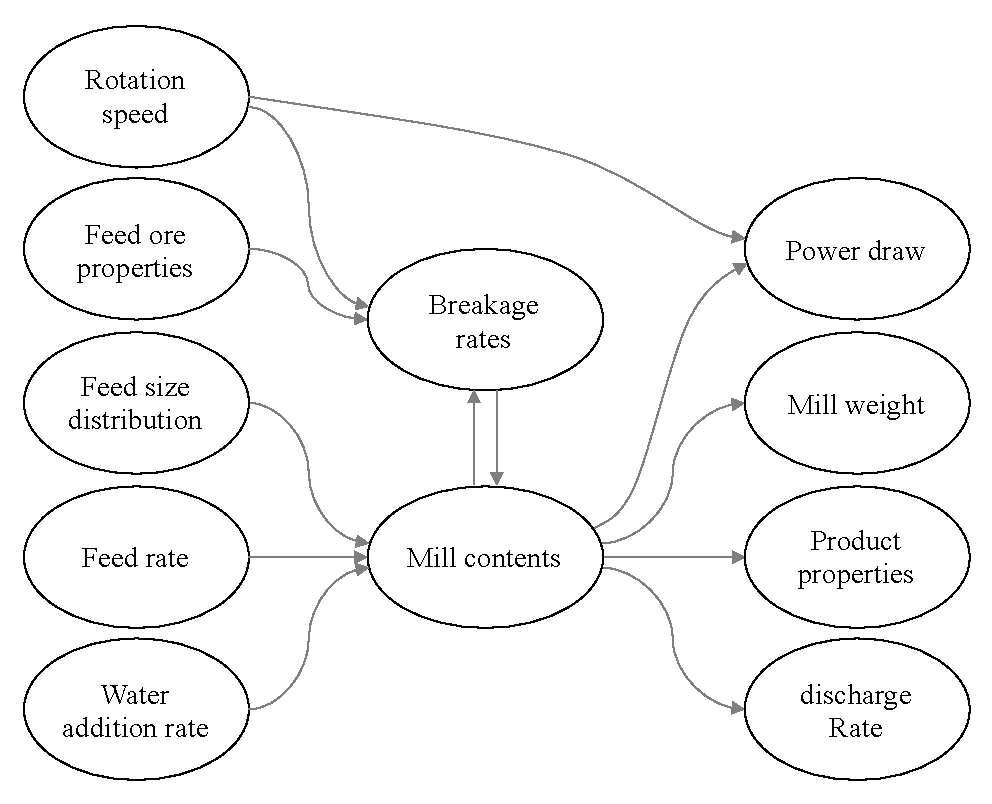
\includegraphics[width=9cm]{images/cause-effect.pdf}
	\caption{Cause and effect diagram} \label{fig:cause-effect}
\end{figure}

Possible references for above:
\begin{outline}
	\1 Papers introducing grinding control problems, references to ore feed disturbances, and surveys on process control in mineral processing.
	\2 Herbst et al (1984) - optimal control potential in grinding
	    \2 Hahne, Palsson, Samskog (2002) - AG effects.
	\2 Powell and Mainza (2006), Powell et al (2009) - grind curves
	\2 Wei and Craig (2009) - control methods survey.
	\2 Hodouin, et al. (2011). Methods for automatic control, observation, and optimization in mineral processing plants.
	\2 McClure and Gopaluni (2015) - Overload Detection in Semi-Autogenous Grinding.
	\2 Olivier and Craig (2017) - degree of automation survey
	\1 Papers on observers for mineral processing applications — E.g. 
	\2 Chen et al (2009) - Disturbance Observer Based Multi-Variable Control of Ball Mill Grinding Circuits. % chenDisturbanceObserverBased2009
	\2 Olivier, Huang and Craig (2012) - Dual particle filters for state and parameter estimation.
	\2 LeRoux et al (2016) - State and parameter identifiability, EKF observer.
	\2 LeRoux et al (2016) - Nonlinear observability of grinding mill.
	\2 LeRoux et al (2017) - An EKF observer to estimate semi-autogenous grinding mill hold-ups.
	\1 Papers on grinding process control and including simulations with ore feed disturbances.
	\2 Najim, Hodouin, Desbiens, (1995) simulated an adaptive controller applied to a grinding circuit with a disturbance in the ore hardness (-20\% reduction in breakage rates) and it's effect on the CVs, product P80 and circulating load.
	\2 Pomerleau et al. (2000) - survey of control, DYNAFRAG simulations.
	\2 Chen, Yang, and Li, (2009). Disturbance Observer Based Multi-Variable Control of Ball Mill Grinding Circuits. (They simulated the effects of a 10\% increase in ore hardness on P80 and circulating load).
	\2 Aguila-Camacho, Le Roux, et al (2017) - fractional order controller and grinding circuit with a change in the mill feed size distribution.
	\2 Botha, le Roux, Craig, (2018) - Hybrid Non-Linear MPC of a Run-of-Mine Ore Grinding Mill Circuit.
	\2 LeRoux et al (2016) - Non-linear MPC.
\end{outline}

\section*{Disturbances}

Outline notes:

\begin{itemize}
	\item Definition of a disturbance — unmanipulatable inputs to process.
	\item Measured v. unmeasured (and unpredictable)— measured disturbances can be incorporated in a feed-forward control.  Unmeasured disturbances must be estimated in order to reject them.
	\item Importance of considering disturbances in control system design.
	\item Disturbance models and process observers.
	\item \textbf{Should this section go in Method chapter?}
	\item Two categories of disturbances: Infrequent, always-present.
	\item Infrequent disturbances could have significant impact on process and control systems (MacGregor et al).
	\item Standard approaches to system identification do not consider infrequent disturbances (focus on second order properties)
	\item Need for broader range of disturbance model types and ways to incorporate them in control strategies.
\end{itemize}

\section*{Background and objectives}

This project is part of a three-year research and development project by the \textit{Laboratoire d’observation et d’optimisation des procédés} (LOOP) of the University of Laval, with financial support from the Government of Quebec and Nemaska Lithium Corporation. The overall goal of the project is to determine the extent to which technological innovations could transform the current paradigm of mineral processing which is energy intensive and results in significant greenhouse gas emissions. The project consists of two main initiatives:

\begin{enumerate}
	\item Development of dynamic operating models of production units
	\item Development of circuit configurations, process controls, and real time optimization strategies.
\end{enumerate}

Aligned with the second initiative, the specific goals of this research project are to identify or develop disturbance models and observers tailored specifically to the types of disturbances and measurement challenges that exist in real mineral processing operations.

The specific objectives of this research project are:

\begin{enumerate}
	\item Propose a model for representing disturbances in mineral processing operations
	\item Propose an observer framework using this model.
\end{enumerate}

\section*{Literature review}

Outline notes :

\begin{itemize}
	\item Describe literature search
	\item Only a gew works found on characterising and modelling disturbances
	\item Significant branch of research on fault/anomaly detection (e.g. Willsky (1976), (1986), Thornhill et al (2007)).
	\item Distinction between detection of anomaly and continued estimation with realistic models.
	\item Papers on disturbance model design for process control tend to consider standard stochastic disturbance models - e.g. Badgewell and Muske (2002), Pannochia (2007).
	\item Exceptions include works on disturbances in specific applications – e.g. wind power, vehicle suspension, waves in ship movement control.
	\item Example: Highlight Papaefthymiou and Klockl (2009) on using MCMC to model wind power generation.
\end{itemize}


A comprehensive search of the academic literature was carried out to identify previous work relevant to the project. During this process it became apparent that the number of works related to characterising and modelling disturbances was quite small. With a few exceptions, searches for terms such as `disturbance model' or `disturbance characterisation' tended to result in works dealing with the design of standard stochastic disturbance models, for example \cite{muske_badgwell_disturbance_2002}, and \cite{pannocchia_robust_2003}, or were focussed mainly on detection and diagnosis of disturbances rather than their simulation or modelling, \cite{thornhill_advances_2007} for example. There is a rich body of work on the subject of fault detection which falls into the second category. In these works, models of the process are used to identify when an \textit{unmodelled} disturbance occurs and to determine its source. However, a typical fault detection algorithm does not have a model of the actual disturbance, therefore its operation is suspended once the disturbance occurs. In contrast, the goal of this work is to identify a model that can be used for state estimation in the presence of disturbances, without interruption.

Some of the exceptions were works on disturbances in specific application domains such as wind power generation, bump disturbances in vehicle suspension systems, and wave disturbances in ship movement control.  In these, researchers developed disturbance models tailored to these applications. For example, \cite{papaefthymiou_mcmc_2008} used a Markov-chain Monte Carlo (MCMC) method to identify and model important characteristics of the wind to generate `synthetic' wind data for the purposes of running realistic dynamic simulations of renewable energy generation systems.

Nevertheless, a small number of research papers were discovered dealing with `realistic disturbances' (loosely defined) occurring in continuous industrial processes. These are also sometimes broadly referred to as `deterministic disturbances' to distinguish them from standard disturbance models based on zero-mean random noise signals (which are truly random in the sense that they are independent and identically-distributed).

\section*{Randomly-occurring deterministic disturbances} \label{RODDs}

\begin{itemize}
	\item MacGregor et al (1985) - is the earliest work on infrequently occurring (non-linear) disturbances.
	\item Many types of RODD can be generated with this model - e.g. steos, ramps, exponential changes.
	\item Examples of applications – operator set-point changes, changes to load on a system.
	\item Here 'deterministic' means not random in the sense of i.i.d.
	\item They show that the optimal control law for a process perturbed by a RODD is no different than that perturbed by an equivalent stochastic noise process.
	\item This is due to the common ARIMA structure and the zero-mean of the random shock. 
\end{itemize}


In 1984, \cite{macgregor_duality_1984} introduced the concept of the \textit{randomly-occurring deterministic disturbance} (RODD). This is a family of stochastic processes useful for modelling deterministic disturbances commonly encountered in real industrial processes. Three types of RODD process are described by MacGregor and co-workers. One produces infrequently-occurring step changes, another produces a series of ramps, and a third produces a signal consisting of a series of exponential changes. One example of a real-world disturbances that might be represented by these models is that of an unanticipated set-point change made by an operator. Another is an sudden unexpected change to the load on a system. While these disturbances may be deterministic, the key issue is that they are not predictable or measurable by the control system. Therefore, simulating them with a stochastic process driven by a random variable is a reasonable way to emulate their unpredictability for the purposes of control system design.

The structural form of a RODD model is an \textit{autoregressive integrated moving average} (ARIMA) process fed by a special \textit{random shock} signal which has the value 0 most of the time but occasionally, according to a defined probability, has a value sampled from a normal distribution. Depending on the chosen ARIMA process model, this can be used to simulate the different types of RODD disturbances which may act on a process. The details of the RODD model are described in section \ref{subsec-RODD}.

MacGregor and coworkers also showed that the optimal control law derived for a process perturbed by a RODD is no different than that which would be derived for a process subject to a standard stochastic noise.  This is due to the common ARIMA structure of both models and the fact that the expected value (i.e. mean) of the random shock signal is zero as it is for a Gaussian noise. As a result, it is well-suited for use in process control design. For this reason, and in the absence of other alternatives, the RODD disturbance model became a focus of this research project.

\section*{Detection and estimation of RODD disturbances}\label{detection_RODDs}

\begin{itemize}
	\item Robertson et al (1995, 1998) - explanation of the trade-off that must be made with a single Kalman filter.
	\item Limitations of traditional models in state estimation of switching systems.
	\item Use of multi-model approach to estimate RODDs online.
	\item Approximations are needed.  Describe the three used by Robertson et al. (dropping low-probability combinations, sequence fusion, and maximum number of shocks in an interval).
	\item Earlier references on multi-model state estimation: Blom and Bar Shalom, Ackerson and Fu, Buxbaum and Haddad, Jaffer and Gupta, Akashi and Kumamoto.
	\item Note slight difference in Robertson RODD model with two random noise inputs.
	\item They compare their multi-model observer with a standard Kalman Filter. How is it tuned?
	\item Summarise simulations and results of the 1995 and 1998 papers (the 2nd is better, it includes MSE comparisons).
	\item Eriksson and Isaksson (1996) - Disturbance model detection. E.g. to determine if the disturbance is at the input or output of the process.
	\item Two sets of Kalman filters combined into one multi-model observer.
	\item They use the AFMM algorithm - uses sequence pruning instead of sequence fusion. Goes back to Andersson (1985) and Gustaffson (1993)
\end{itemize}

Traditional filtering methods such as Kalman filters are unable to efficiently estimate RODD disturbances due to the inevitable trade-off that must be made between the ability to track a disturbance when it occurs and the sensitivity to noise \cite{robertson_detection_1995}.

Prior work in the field of process monitoring focused on the problem of fault detection. The disadvantage of these methods was that, once a fault is detected, the estimation process stops, and some sort of corrective action is required before the filters can be restarted. 

In their 1995 paper, Robertson, Kesavan and Lee \cite{robertson_detection_1995} described how unmeasured RODD disturbances perturbing a system can be estimated online using a \textit{multi-model} observer approach that is effective over an extended period of time during which any combination of several disturbances may occur.

Multi-model filtering approaches involve simultaneously computing multiple independent filters with different parameters and then combining the estimates from these filters to produce a better estimate of the system states \cite{jaffer_estimation_1971, buxbaum_recursive_1970, tugnait_detection_1982}.

Unlike the random shock signal defined by MacGregor and co., Robertson and co. use a signal that is sampled from one of two normal distributions, one with a low variance and the other with a much higher variance. This means that the probability density of the shock signal is conditionally Gaussian, whereas the shock signal used by MacGregor and co. has a non-smooth (i.e. degenerate) probability density function.

Since the sequence of past random shocks is not known, each filter's state estimate is calculated assuming a different sequence of past possible shocks. The estimates of some filters are therefore better than those of others, depending on how closely the shock indicator sequences match the disturbances that actually occurred. The overall best estimate of the states is computed by calculating the conditional probabilities of each indicator sequence given the available measurement data, and this estimate is updated recursively each sample period using Bayesian inference.

Due to practical limitations, the optimal multi-model approach cannot be implemented and some kind of approximation is needed to limit the number of filters required. Practical multi-model observers are therefore referred to as \textit{sub-optimal}. Robertson and coworkers propose using a combination of three specific approximations when estimating RODD disturbances.

The first is based on the assumption that correctly estimating the exact timing of RODD disturbances is not important and therefore a filter that assumes a shock occurred within a short period close to the actual occurrence will be adequate. This is based on the observation that when the correction gain of a Kalman filter is increased at time $k$ due to the assumption of a shock occurrence, it tends to remain large for several sample periods thereafter.

The second approximation is based on the assumption that RODD disturbances occur infrequently and it is quite unlikely that two or more shocks occur within a short time period. This further reduces the number of filters required, especially in systems subject to multiple independent disturbances.

The third approximation is referred to as \textit{filter fusion} or the \textit{generalized pseudo-Bayes algorithm} \cite{jaffer_estimation_1971, buxbaum_recursive_1970, tugnait_detection_1982}. This is based on the assumption that only differences in the recent values of the shock indicator sequence affect the state estimates. Therefore, sequences whose last $f$ terms are the same can be combined. In other words, the length of the unique sequences which must be maintained is limited to the previous $f$ sample periods.

Robertson and coworkers present results of simulating their sub-optimal multi-model observer on a 2-input, 2-output, non-linear dynamical system representing a continuous stirred-tank reactor (CSTR) process. They show the estimates produced by the multi-model approach compared with two single extended Kalman filters (EKF) with different noise parameters. The first of the single EKFs is sensitive to the measurement noise and the second is slow to respond to the RODD step disturbances, while the multiple-model observer appears to perform better than either single EKF in the example simulations.

A year later, Eriksson and Isaksson \cite{eriksson_classification_1996} present results of using an adaptive multi-model approach to estimate \textit{infrequently-occurring disturbances}. They utilize the \textit{adaptive forgetting through multiple models} (AFMM) algorithm by Andersson \cite{andersson_adaptive_1985} and also previously described by Gustafsson \cite{gustafsson_estimation_1993}. The AFMM algorithm employs a technique called \textit{sequence pruning} \cite{tugnait_detection_1982}, in contrast to the sequence merging or fusion technique used by Robertson and co.\cite{blom_interacting_1988}.

Sequence pruning is the online deletion of sequences that have a low probability given the current measurements. The deleted sequences are replaced by new sequences to represent the possible branches of the most likely sequence at the next sample time. For example, for a system with one infrequently occurring input disturbance, the most likely shock sequence at the next sample time is the shock sequence estimated to be most likely at the current time extended by the addition of a zero to indicate no shock at the next sample time. However, a shock could occur in the next time period. To account for this possibility, a new shock sequence is generated by making a copy of the current most likely sequence and its associated filter and extending it assuming a shock at the next sample time. This new sequence and filter replace the least likely sequence and observer. Thus, the total number of sequences and independent filters that need to be maintained remains constant. Note that in the case of systems with more than one input disturbance, the number of possible branches of the most likely sequence is higher, and therefore a larger number of sequences and filters will be replaced each time step.

There is one restriction to this pruning rule. A sequence created at sample time $k$ cannot be deleted until sample time $k+n_{min}$ where $n_{min}$ is a \textit{minimum life length} parameter. This is necessary because it can take several sample periods before the filter estimates respond to the change and thus the conditional probability of the new sequence is established.

The AFMM algorithm also includes a procedure for online estimation of the measurement noise covariance, using a forgetting factor to control the speed of adaptation of the estimate.\cite{andersson_adaptive_1985}

In Robertson and co., the RODD disturbance model is assumed to be known. This is also the case in Eriksson and Isaksson's paper, however, Eriksson and Isaksson show how the estimation procedure can be extended to discriminate between two possible disturbance hypotheses. They consider the example of determining whether a step disturbance is affecting the output or the input of the process, assuming it is actually present at either but not both simultaneously.

Two sets of Kalman filters are run simultaneously, one set with the infrequently-occurring disturbances modelled at the input of the process and the other set with them modelled at the output. The conditional probabilities of all filter models are calculated every sample time and normalized across both sets of filters.  Thus an online estimate can be made of which disturbance hypothesis is most likely (i.e. an input or output disturbance) as well as an estimate of the magnitude of the disturbance. They provide results from simulated examples and a laboratory experiment to show that the AFMM method correctly estimates the disturbance actually present in each case.

Robertson and Lee published a second paper in 1998. In this paper they list Anderson \cite{andersson_adaptive_1985} among the references on multiple-model algorithms.  However, the approach and sub-optimal method used is essentially the same as in their 1995 paper, with only slightly different terminology used (`infrequently occurring abrupt disturbances' instead of `randomly occurring deterministic disturbances'). 

However, a different non-linear system (a 3-state model of a heptane to toluene aromatization process) is used for the numerical example and, importantly, this time sum-of-squared errors for the parameter estimates are presented averaged over 50 Monte Carlo simulations, so it is easier to compare the different methods. They compare their sub-optimal method with a single EKF and with the generalized pseudo-Bayes (GPB) algorithm (without sub-optimal modifications).

The results show that their sub-optimal filter does 35 percent better than either the EKF or the GPB algorithm. This is simply because their filter has a horizon of 90 minutes (using 22 filters), whereas the standard GPB algorithm has a horizon of only 2 minutes (using 16 filters) so there is not enough time for it to detect changes before the filters are fused.

\section*{Disturbance modeling using hidden Markov models}
\label{hidden_markov_models}

Outline notes:

\begin{itemize}
	\item \textbf{TODO: Much of this we could drop since we did not look at HMM models.}
	\item Wong and Lee proposed a generalized framework for modeling realistic disturbance processes which have both continuous and discrete (i.e. modal) dynamics \citep{wong_disturbance_2007}.
	\item The mode transitions are described by a finite-state \textit{Markov chain}.
	\item The model generating the Markov chain is referred to as a \textit{hidden Markov model} (HMM) because it is unknown and must be inferred from available noisy measurements.
	\item The combined system including discrete and continuous dynamics is termed a \textit{Markov jump linear system} (MJLS) \citep{costa_discrete-time_2005}.
	\item Wong and Lee point out that the application of HMM's and MJLS's in science and engineering is not novel and refer readers to the references in \cite{costa_discrete-time_2005} for prior work by the control community. Nevertheless, they claim that the use of HMMs for disturbance modeling prior to 2007 was limited.
	\item They also note that the RODD disturbance model of Robertson and Lee, and other methods assuming noise inputs described by \textit{mixture-of-Gaussians} (MOG), can be considered special cases of the MJLS.
	\item Unlike Robertson and Lee, who focused on state estimation, Wong and Lee are interested in identification of the model in the presence of non-stationary noise.
	\item Wong and Lee show how the plant and Markov chain parameters may be simultaneously estimated by \textit{maximum likelihood estimation}, specifically, using the expectation maximization (EM) algorithm (see section \ref{mle}).
	\item In their numerical examples, Wong and Lee use a second-order generalized pseudo-Bayesian (GPB2)  method for state estimation \citep{bar-shalom_estimation_1993} (see section \ref{gpba}).
	\item The first example in their 2007 paper, is a disturbance that switches infrequently between a white noise and an integrated white noise.
	\item They compared the prediction errors of a GPB2 observer using the identified MJLS model to those of the best observer with a stationary (i.e. non-switching) model, as well as to those of a GPB2 observer which uses the actual system model.
	\item The 1-step-ahead prediction errors of the GBP2 with the identified model were 26 percent lower than the optimal stationary-model observer and only 7 percent worse than those of the GBP2 with the true model.
	\item These results are averages over 500 simulated realizations, each of 2000 sample periods in length.
	\item The second example is a `soft-sensor' approach for inferential control where the system is subjected to two integrated noise disturbances at the output, each switching between two noise levels with certain probabilities. In this example, the simulation results indicated that the 1-step-ahead prediction errors of the GPB2 observer with the identified model were only 6 percent higher than a GPB2 observer with the true model.
	\item The main limitation of the results presented in the 2007 paper is that they only test the method on systems which switch only in their noise parameters.
	\item The other limitation that they acknowledge, is that the MLE optimization is non-convex and hence may not converge to the global optimum. To mitigate this problem, they chose initial values `suitably close' to the true system parameters.
	\item Although Wong and Lee do not refer to it, it's worth noting that Elliott, Aggoun, and Moore wrote a book on hidden Markov models for estimation and control in 1995 \cite{elliott_hidden_1995}. A central theme of this book is use of so-called \textit{reference probability methods} for optimal estimation and control which they claim are accessible to non-specialists.
	\item Reference probability methods involve a change of probability measure (they are also known as the \textit{measure change approach}) which allows the original estimation and control problem to be reformulated so that well-known results for \textit{identically and independently distributed} (i.i.d.) random variables can be applied, thus simplifying the analysis and the computational complexity. \emph{TODO}: where does this approach fit in with the other concepts (e.g. in Costa's book) and is it still relevant today?
	\item Hybrid systems (e.g. 1999 book by Sworder and Boyd on estimation of hybrid systems)
	\item Discrete time Markov Jump Linear systems (MJLS) (Costa 2005 book)
	\item Problems of observability and Identifiability of Jump Linear Systems (Vidal et al. 2002).
	\item Bemporad on identification of switching systems - e.g. mixed-integer programming (2001), jump models (2018), jump Box-Jenkins model (2020)
	\item Other estimation methods—particle filtering (Arulampalam, 2002 tutorial).
	\item Control of processes subject to intermittent disturbances. MacGregor - duality, Costa book (2005), Wong and Lee efforts (2007), (2009), (2020), (2011), Camacho et al. ()2010).
	\item TODO: Explain field of sequential Monte Carlo techniques (includes particle filtering, EM, etc.).  Holistic view.
\end{itemize}

\section*{The hidden Markov model for process control}
\label{hmm_control}

Outline notes:

\begin{itemize}
	\item \textbf{TODO: Should I include this summary of application of HMM to process control?}
	\item Wong and Lee's 2009 paper \cite{wong_realistic_2009} goes further than their 2007 paper \cite{wong_disturbance_2007} by demonstrating how the proposed HMM-based disturbance framework can be integrated into existing model-based control formulations.
	\item After introducing the HMM framework again, they present 3 numerical examples demonstrating the use of the framework in process control methods and applications, including one to mitigate the impact of highly-varying feed streams entering an ethanol-producing bioreactor.
	\item They provide only a brief review of system identification methods for Markov jump systems and note that it was still an open area of research at the time.
	\item Due to the difficulties of MJLS identification, they bypass the issue in this paper, and assume that the system, noise and Markov parameters are available.
	\item As in the 2007 paper, they use the second order Generalized Pseudo-Bayesian algorithm (GPB2) developed by Bar-Shalom \cite{bar-shalom_estimation_1993}.
	\item Although they don't use it, Wong and Lee also mention the interacting multiple model (IMM) algorithm which they say has a similar performance as GPB2 but at the computational cost of GBP1 \cite{wong_realistic_2009}. \textbf{TODO}: Need to see where this fits in.
	\item The GPB2 algorithm is a recursive estimation scheme, characterized by `branching' and `merging' steps. Wong and Lee provide a simple numerical example of the algorithm including plots of the output and state estimates. Refer to Fig. 3 in \cite{wong_realistic_2009}.
	\item The first of the three examples in the 2009 paper demonstrates the use of the HMM disturbance framework for offset-free linear model predictive control (LMPC) on a single-input, single-output system.
	\item Four simulation scenarios are considered for this example: low input noise compared to output noise, high input noise compared to output noise, similar input and output noise levels, and switching levels of input and output noise (all simulations were run with negligible measurement noise).
	\item In order to investigate model-plant mismtch, four different model-predictive controller/estimator pairs were constructed: one with an output disturbance only, one with only an input disturbance, one with both input and output disturbances, and the fourth with switching behaviour (using the GPB2 estimator).
	\item For each of the four simulation scenarios, 500 realizations, each of duration 500 sample periods, were run and a controller coupled with a time-varying Kalman filter assuming perfect knowledge of the true simulation regime was simulated for benchmarking purposes.
	\item Each controller is evaluated by the average ratio of its squared-tracking error and that of the benchmarking controller/estimator.
	\item The simulation results show that the proposed MPC designed with the HMM model and GPB2 estimator yields the best performance over all simulation scenarios.
	\item Example 2 demonstrates the closed-loop performance of the HMM control approach in detecting and rejecting deterministic step changes.
	\item The controller's performance is compared to a well-tuned controller based on the \textit{integrated white noise} (IWN) approach to rejecting such perturbations.
	\item The results show that the HMM framework achieves an increase of only 6 percent in the error when compared to the ideal full-feedback controller, and yields better performance than a well-tuned IWN-based estimator.
	\item The third example concerns the control of a nonlinear ethanol fermentation process simulation model where the HMM framework is used to represent the highly-varying nature of the feed concentrations.
	\item The glucose concentrations entering the process are modelled as fluctuating among several mean levels (low, mid and high) and the transitions are governed by a Markov chain.  The problem is such that the regime transitions are infrequent since changes in feed type/quality tend to occur on time scales that are longer than that of the plant’s dynamics.
	\item A \textit{sequentially-linearized MPC}, which is a computationally attractive alternative to a full non-linear MPC implementation \cite{lee_extended_1994}, is used to evaluate the closed-loop performance.
	\item The effect of different types of feedback is compared: Full state feedback including the Markov decision variable; Markov decision variable and output feedback only, and output feedback only (corrupted by measurement noise).
	\item As in the previous example, a controller/estimator pair that operates on the common assumption that the disturbance is integrated white noise (IWN) is used as a benchmark.
	\item Not surprisingly, the results indicate that the amount of information available to the controller determines the closed-loop performance, especially, knowledge of the Markov state trajectory. However, all three HMM-based approaches are better than the benchmark closed-loop system relying on the output measurements only.
	\item The authors concluded that the benefits of an HMM-based disturbance framework are ``most immediately reaped" by incorporating them within existing control methodologies such as MPC, as opposed to the optimal control policies developed specifically for Markov jump systems, such as those described in \cite{costa_discrete-time_2005}.
	\item Finally, they stated that the development of systematic model identification methods and more robust control algorithms for Markov jump systems was the focus of their ongoing research.
	\item In 2011, Wong and Lee published a conference paper on the HMM framework for disturbance modelling in which they present the framework again. Again they use the GPB2 algorithm for sub-optimal filtering and present results of two numerical examples. One for state estimation with abruptly changing feed conditions for a `second generation' bioethanol fermentor, and the second for the case of tracking stiction in a mechanical valve, which is a non-trivial detection problem.
	\item As in the previous papers, the results show better performance for the HMM-based approaches.
\end{itemize}


\section*{Contributions of this research}

The main contributions of this research are:

\begin{enumerate}
	\item A review of academic literature pertaining to `realistic' disturbance modelling and state estimation in industrial process operations.
	\item Evaluation of the capabilities of two multi-model observer algorithms by simulations in MATLAB.
	\item Evaluation of the performance of one of the multi-model observers applied to state estimation of a simulated grinding process.
	\item Evaluation of the benefits of one of the multi-model observers as part of a simulated control system applied to the simulated grinding process.
	\item T.b.d.: A case study of the application of model identification techniques to characterise disturbances using data from a real industrial operation.
\end{enumerate}

\section*{Organisation of this report}

Chapter 1 describes the methods used in the research including the disturbance model, the observer designs and the grinding simulation model used for evaluation of one observer.  Chapter 2 describes the simulations carried out to demonstrate the disturbance model and to evaluate the performance of the observers (TODO: And to estimate the potential benefits?). Chapter 3 describes simulations carried out to test some of the possible methods to identify and characterise disturbances from measurement data.
          % introduction
% !TEX encoding = UTF-8 Unicode
\chapter{Literature review, objectives, and contribution}
\label{chap-lit-review}

The literature review was in two parts. The first part, which is summarised in Section \ref{sec:lit-grinding}, describes previous research related to grinding process control. This includes an introduction to the dynamics of the grinding process and work on grinding process control, process observers, and grinding process disturbances. This informed the objectives of the work which are described in Section \ref{sec:objectives}. Section \ref{sec:lit-disturb-models} is the second part of the literature review, which focussed on industrial process disturbance models, observers for estimating disturbances, and other methods related to the work. Section \ref{sec:contributions} lists the main contributions of this research.

\section{Literature review part 1 – grinding process control} \label{sec:lit-grinding}

\subsection{The grinding process}

Figure \ref{fig:cause-effect} is a schematic diagram illustrating the main cause-effect relationships in a tumbling mill. Each oval represents an important process variable and the arrows represent the interacting relationships and the direction of causality. The five variables on the left are the main input variables and the four on the right are the main outputs or measurements. Mill contents and breakage rates are internal variables of the process. Here, mill contents has a broad definition encompassing all attributes of the contents, including water, slurry, ore particles, and grinding media.
\begin{figure}[htp]
	\centering
	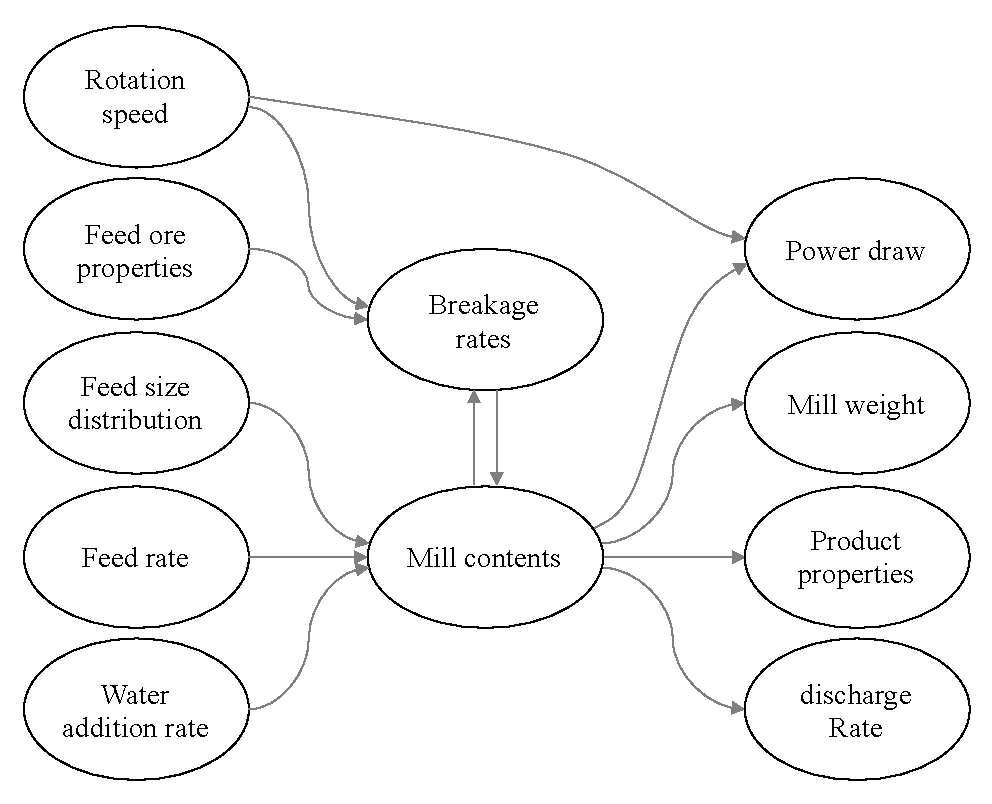
\includegraphics[width=11cm]{images/cause-effect.pdf}
	\caption{Cause and effect diagram} \label{fig:cause-effect}
\end{figure}

\cite{powell_applying_2009} highlighted the interactive (i.e. bi-directional) relationship between mill contents and breakage rates and describe how these variables evolve dynamically. A change in ore feed properties, such as a change in hardness or particle sizes, leads to changes in the mill contents, which then affect breakage rates, which have a feedback effect on the evolution of the mill contents. This results in a non-linear response of the output variables that depends on the mill contents.

As mentioned in the introduction, changes in ore feed properties have a significant impact on the process. \cite{morrell_influence_2001} stated that variations in ore competency and the feed size distribution are the top two factors having the greatest influence on \acrshort{SAG} mill performance.

\acrshort{SAG} mills are usually installed in closed-circuit with a pump and a classifier, as in the example shown in Figure \ref{fig:sag-ball-circuit-diag}. Oversize material that passed through the discharge grate of the mill but does not meet the specification of the classifier is returned to the mill, sometimes via a crusher. This feedback mechanism has a transport delay, which further complicates the dynamic response of the process variables to changes in the inputs.

\subsection{Grinding process control}

The objectives of process control in grinding applications are firstly, to maintain a steady operation and secondly, to optimize the process conditions to maximize operational benefits, for example, maximizing throughput while meeting the product particle size specification \citep{wei_grinding_2009}. Inevitably, trade-offs must be made between competing output objectives, such as throughput and product particle size, and between product particle size and power consumption. The focus of this work is to identify and develop methods that facilitate the first objective (i.e. steady operation) given a set of desired operating conditions.

According to a 2007 worldwide survey of grinding circuit operators \citep{wei_grinding_2009}, 63\% reported that the \gls{PID} control was used. \textit{Multivariable control} or \textit{expert systems} were used by 21\%. Less than 10\% reported using \gls{MPC} or adaptive (self-tuning) control.

The three most commonly controlled variables are the product particle size, the slurry level in the sump, and the sump discharge slurry density. The mill load or filling level also requires some form of control since excursions above or below the normal range can lead to undesirable conditions such as \textit{mill overload} and \textit{freewheeling} \citep{mcclure_overload_2015}. If the load becomes too high, the mill may have to be stopped, resulting in lost production \citep{wei_grinding_2009}.

The main manipulated variables used for control are the set points of the water flow rate to the sump, the water flow rate to the mill, the feed rate of solids to the mill, and the slurry discharge flow rate from the sump. Many modern mills also have variable speed drives which allow controlled variation of the rotational speed. However, use of speed as a manipulated variable was reported by less than 10\% of respondents in \cite{wei_grinding_2009}.

There is an extensive academic literature on the application of process control theory and methods to grinding, going back as far as the 1980s, e.g. \cite{herbst_optimal_1988}. A wide variety of techniques have been proposed and evaluated since then. Most of the results are based on computer simulations of control systems applied to simulation models of grinding processes. In many cases, these simulations include ore disturbances.

\cite{najim_adaptive_1995} simulated various adaptive controllers applied to a grinding circuit model with a step disturbance in the ore hardness, represented by a 20\% reduction in breakage rates. In their work, the controllers regulate the circulating load and product size by manipulating the water addition rate and the fresh ore feed rate.

\cite{pomerleau_survey_2000} simulated various control algorithms applied to a grinding process consisting of a rod mill and a ball mill. The controllers manipulated the set points of the fresh ore and the water feed rate to regulate the product fineness and the circulating load. To compare the performance of the controllers, they simulated a sequence of disturbances to two ore properties---\textit{grindability} and feed size---as well as a change in the number of active cyclones, and set-point changes to controlled variables.

\cite{chen_disturbance_2009} proposed a \gls{DOB} control strategy applied to a ball mill grinding circuit model and evaluated its effectiveness in suppressing the effects of a 10\% increase in ore hardness on the product fineness and circulating load.

\cite{estrada_hybrid_2014} simulated a \gls{HNMPC} system to minimize specific energy consumption while regulating the product particle size. Hybrid approaches allow discrete variables to be included in the plant model. These are useful for representing processes which have discrete operating modes, such as those with equipment items that may be switched on or off during operation. They used this to represent changes in the stockpile feeding process and the activation of secondary grinding circuits. They presented simulation results showing how the controlled system responded as the different ore feed streams were switched off and on.

\cite{le_roux_throughput_2016} simulated a non-linear model-based control architecture to independently control the throughput and product quality of a grinding circuit. To achieve this, they used the set points for mill speed, feed rate, water addition, and cyclone feed-rate as manipulated variables.

\cite{botha_hybrid_2018} simulated a \gls{HNMPC} system for a primary grinding mill circuit in which the number of hydrocyclones (a discrete variable) is used as an additional manipulated variable. The switching of hydrocyclones has a large dynamic influence on the plant. They show that this increased controller stability compared to nonlinear \gls{MPC} without this discrete variable.

\cite{aguila-camacho_control_2017} simulated various types of \textit{fractional order controllers} applied to a grinding circuit model with five manipulated input variables (fresh ore feed rate, mill inlet feed water rate, sump feed water rate, cyclone feed flow rate, and ball addition rate) and three output variables (mill filling level, sump slurry volume, and product fineness). They also simulated step changes in the ore feed size distribution and in energy required to break ore particles, which is similar to ore hardness.

There is less literature available on the implementation, performance, and benefits of control systems in actual operations.

\cite{herbst_optimal_1988} presented results of implementing an optimal control algorithm (\gls{LQG}) on a rod and ball mill grinding circuit in North America. This included use of an extended Kalman filter to estimate the states and parameters of a non-linear phenomenological model. The results show that the observer estimates tracked the process output measurements in response to a change in ore hardness, and the corresponding changes in model parameters.

\cite{hulbert_multivariable_1990} presented results of implementing a multi-variable controller on an AG mill in South Africa. The manipulated variables were set points for the ore feed rate to the mill, the water feed rate to the sump, and the flow rate of slurry to the cyclone. The controlled variables were product particle size, mill load, and slurry level in the sump. The results show the responses of the controlled system to set-point changes. They state that implementation of the multivariable controller resulted in better control of the product size and an increase in throughput.

\cite{desbiens_distributed_1997} described the development and implementation of a \gls{PI}-based regulatory control strategy on a grinding circuit at a mine in Ontario, including the steps of process model identification and filter design. The installed system regulates the pump box level, the cyclone feed density and the cyclone overflow density by manipulating the pump box water addition set point, the rod mill water addition set point, and the rod mill ore feed rate set point.

One of the case studies presented by \cite{desbiens_using_2008} described the implementation of an improved grinding circuit control strategy in a copper concentrator in Peru. They addressed the problem of quickly adjusting the rod-mill feed rate when a change in ore hardness occurred. This was achieved by simultaneously manipulating the rod mill feed rate and a flow splitter controlling the flows to the ball mills according to the levels in the pump boxes. After implementation of the new control system, the variability in process conditions reduced, the average throughput increased by 4\%, and the combined circuit energy consumption reduced by 8\% to 10\%.

\cite{nunez_self-optimizing_2009} described the development and implementation of regulatory controls at a mine in Canada. The grinding process consisted of two parallel circuits, each containing an open-circuit rod mill and a ball mill in closed-circuit. They reported that ore hardness changes were leading to either over or under-grinding and mill overload situations, which were not always detected in time by the operators. The new system consisted of two distributed control loops on each circuit, one to control the pump-box level by manipulating the rod mill feed set-point, and the second to control the cyclone overflow density (in the absence of a product particle size analyser) by manipulating the pump box water addition rate set-point. The results indicated a significant (60\%) reduction in variability of the product density and a 7.7\% increase in throughput for the same level of energy consumption, no change to mineral recovery, and the avoidance of mill overloads.

\cite{yutronic_sag_2011} described the development and implementation of an \gls{MPC}-based control strategy at a large concentrator plant in Chile. The primary goal was to reduce process variability in the \acrshort{SAG} circuits, and in particular, the effects of poor sump level control on classification efficiency. The \acrshort{SAG} filling level was deemed to be the most important process variable, due to its relationship with grinding efficiency. Since filling level is not measurable, the mill weight was used as the controlled variable, along with the power draw, the shell impact noise level, the motor torque, and the produced pebble flow rate. The \gls{MPC} included constraints on certain process variables, such as the power draw to avoid electrical overload. The manipulated variables were the fresh ore feed rate set point, mill speed set point and the solids-to-water ratio of the feed. Two measured disturbances were also included in the \gls{MPC} model, the returned pebble flow rate and the fine ore percentage in the feed.

As a result of implementing the \gls{MPC} system, the variability of the cyclone feed solids content and feed pressure were reduced by 43\% and 22\%, respectively. Other benefits included higher throughput, lower specific energy consumption, and a 4.8\% reduction in the average \acrshort{SAG} product size.

\cite{steyn_benefits_2013} presented results of implementing \gls{MPC} on an \gls{AG} mill in South Africa with the goal of reducing variability and to ``continuously drive towards the optimal operating point within system constraints.'' The two main controlled variables were power consumption and mill load. They report a 66\% reduction in power and a 40\% reduction in the standard deviation of the mill load as a result of implementing the \gls{MPC}. This reduction in process variability also enabled steady-state experiments to be conducted to determine the optimal product particle size for a given mill feed rate, which led to a subsequent improvement in mineral recovery.

\cite{gough_sag_2015} reported using \gls{MPC} to control the mill weight, feed rate, and rotation speed of various \acrshort{SAG} mills in mines in South America. The controller included measured disturbances such as pebble recycle rate and ore size distribution as feed forward inputs to improve control. He presented results showing that the \gls{MPC} is able to reduce the variability in mill weight (84\% reduction in standard deviation) and throughput (55\% reduction in standard deviation) compared to the expert systems that were used in these facilities, resulting in increased production.

\cite{bouchard_reducing_2017} showed how a properly designed control system can enable higher utilization of grinding circuit capacity and a reduction in specific energy consumption (\acrshort{kWh}/ton). They used a simulation model of a rod and ball mill circuit to compare three different control strategies. Firstly, a basic \gls{PI} regulatory strategy to control the pump box level by manipulating the water addition set point to the pump box and to control the hydrocyclone pressure by manipulating the cyclone feed rate set point. Secondly, a \gls{PI} regulatory strategy to control the pump box level by manipulating the rod mill feed rate set point, and the product particle size (\acrshort{P80}) by manipulating the water addition set point to the pump box. Thirdly, an \gls{MPC} (multivariable) strategy to control the product size while maximising the rod mill feed rate, using all four manipulated variables. The simulation results demonstrated that controlling the product size ensures not only that downstream process requirements are met and over-grinding is avoided, but can, in some instances, lead to higher throughput and hence, lower specific energy consumption.

\cite{liu_development_2018} analysed the mineralogical aspects of a grinding operation in Western Canada to determine the potential benefits of adjusting mill speed and load to offset changes in mill feed characteristics. However, the analysis was based on a steady-state simulation model and did not look at process control design aspects.

%% Although it mentions ore hardness changes, this is about ball mill process control.

%\cite{nunez_tecks_2019} described a program of process control improvements on the secondary grinding process at a large copper concentrator in Canada.  The ore at this mine is sourced from three main pits and therefore exhibits high variability, including in hardness. While the primary grinding stage is the primary constraint from the perspective of maximising throughput, the objective of the secondary grinding control strategy was to adapt to feed changes to produce the smallest product particle size possible.
%
%The controlled variables were cyclone feed density and ball mill power consumption, and the manipulated variables were pump box water addition rate and ball mill feed water addition rate. The improvements also included a real-time steel charge schedule, and the results show that the system reduced the product particle size from the grinding circuit by 7.5\%.

\cite{steyn_investigating_2018} investigated the potential benefit of an image-based online particle size analyser of the feed to the primary milling circuit. They considered its use in both feedback (reactive) and feed-forward (proactive) control applications, and also as a process monitoring tool for operators. In the feedback case, they assumed that the upstream blasting or ore blending processes could be manipulated to control the feed size. The disadvantage of this approach is the lag time in the response of the system. In the feed-forward case, the information on the feed size was used in the mill control system to compensate for the effects of the disturbance as it impacts the mill. The disadvantage of the feed-forward control strategy is that an accurate model of the process dynamics is needed. They presented results of testing the feed-forward control scheme in two mill operations and reported reduced variance in process variables when the controller was operating, although the statistical significance of the results was deemed to be low.

\subsection{Grinding process observers}

As mentioned above, one of the major obstacles to \acrshort{SAG} mill process control and optimization is the lack of good online measurements (i.e. in real time) of critical process variables, in particular, breakage rates and the characteristics of the mill contents. Of the output variables shown on the right-hand side of Figure \ref{fig:cause-effect}, only power draw is directly measurable. Mill weight may be inferred from load sensors or bearing pressure measurements. However, a reliable estimate of the weight of the mill contents is complicated by the fact that the total mill weight includes the weights of the shell and liners, which change over time due to wear, and the water content. Direct measurement of the properties of the discharge of a \acrshort{SAG} mill is also impractical due to the physical nature of the slurry flow.

Many measurements, such as sump levels and density measurements, are affected by high frequency measurement errors (noise) while others, such as particle size measurements, rely on physical analysis systems which have low sampling rates and are often unreliable. \cite{casali_particle_1998} developed and tested a soft-sensor for online estimation of the product particle size distribution. Although, this is a measured variable, the purpose of their soft sensor was to provide a substitute for the measurements during times when the instrumentation was unavailable.

Process observers that produce reliable online estimates of the unmeasurable variables are an important tool in grinding process control. However, little progress has been made in developing successful methods to infer estimates of important variables, such as the internal states of a mill and the characteristics of the feed ore. Most of the early work on state estimation was on process observers with linear models of the process. These are restricted to a somewhat limited range of operating conditions and cannot accommodate significant changes in grinding conditions or equipment without manual adjustments. Early work by Herbst and colleagues (see, for example, \cite{herbst_model-based_1992}) utilized Kalman filters to estimate grinding process variables such as mill filling, ore hardness, and even breakage rates. However, as \cite{le_roux_ekf_2017} point out, these studies did not explicitly assess the \textit{observability} of the true process states to ensure that the estimates are reliable.

More recently, observers with non-linear or adaptive process models have been investigated. Given the time-varying nature of grinding process parameters, it may be necessary to simultaneously identify both model parameters and states online from measurements. \cite{apelt_inferential_2002} and \cite{apelt_inferential_2002-1} studied the combined state and parameter estimation of a phenomenological model of a \acrshort{SAG} mill. However, they found that the system was not fully observable. Even when numerous measurements of material flows disaggregated into 27 particle size intervals were included, a unique solution for the parameters and states could not be found.

\cite{olivier_dual_2012} simulated the application of particle filtering to the estimation of both model states and parameters (known as \textit{dual estimation}) of a simulated primary grinding circuit and compared this approach to a simultaneous estimation method. The particle filtering approach was selected because of the non-linearity of the grinding model. They tested both approaches in closed loop with decentralized \gls{PI} controllers.

\cite{le_roux_throughput_2016} also investigated a particle filter to estimate the mill states. Their observer only utilises measurements that are commonly available in industrial plants, such as mill power and cyclone feed density.

\cite{le_roux_state_2016} investigated the state and parameter identifiability of a non-linear \acrshort{SAG} mill model including an explicit representation of the mill contents and breakage rates. They used six states to represent the volume of rocks, solids, coarse ore, fines, balls and water (the \textit{hold-up}) inside the mill. However, they found that measurements of the cyclone discharge flow rate and density were necessary for identifiability. Unfortunately, these measurements are not commonly installed in practice.

In \cite{le_roux_ekf_2017}, an \gls{EKF} utilizing a simpler version of the mill model with only three states was used to represent the mill contents (grinding media, solids, and water). They showed that the states and parameters are linearly observable provided the mill discharge flow-rate, discharge density, and volumetric hold-up are measured. However, such instrumentation is also not typically available in industrial circuits due to space restrictions. They also note that the measurements must be sufficiently accurate to reliably estimate the model states.

\subsection{Grinding process disturbances}

Continual variability in ore properties such as hardness, competency, the \gls{PSD}, and grade (valuable mineral content) is normal in mining operations due to the geological characteristics of ore bodies. Additional variability is introduced by mining processes such as blasting and crushing, and during material handling operations such as shovelling, trucking, conveying, and storage. Storage systems such as stockpiles, for example, tend to cause segregation of material by particle size, which can result in dramatic changes in the particle size distribution of ore feeding primary grinding if the feed to the stockpile is interrupted \citep{estrada_hybrid_2014}. The nature of such variations will therefore reflect the particular processes and equipment employed at each site. Although they are not random, the complexities of these systems and their numerous effects and delays make predicting variations in the ore properties arriving at the processing plant extremely difficult.

\cite{morrell_influence_2001} presented data on the influence of feed size distribution on mill performance and discussed the reasons why tumbling mills respond the way they do. They state that \textit{ore competency}, which indicates its resistance to impact breakage, is the main factor impacting mill performance although feed size distribution is a close second. They explain that the sensitivity of \acrshort{SAG} mills to ore feed properties declines as the ball filling is increased. Based on sample data from three different operations, they found that the standard deviation of the feed size (F80) was 15 to 17 mm and the 95\% confidence interval was $\pm30\text{\%}$ of the mean. They also present data from an image-based online analyser which indicated that an increase in F80 caused higher specific energy and consequently lower throughput at constant mill power. They state that as the feed size increases, the mill weight increases, since it becomes increasingly difficult to break the larger rocks. The increased weight causes the power draw to increase. With a constant weight or power draw control strategy, this results in a decrease in throughput.

There is limited available data on actual ore variability in real operations, especially on the dynamic nature of these variations. This may be attributed to the lack of cost-effective measurement technology, the cost of sampling and analysing ore, as well as the commercial sensitivity of such data.

\cite{hahne_ore_2003} carried out tests of ore samples from different points in the production process at a mine in Sweden. The results were used to estimate the influence of feed ore characteristics on grinding performance using a simulation model of the single stage \gls{AG} circuit. The simulation results indicate that the net throughput with a coarse and hard ore was 10\% higher compared to fine and soft ore, and that the fine and soft feed resulted in a coarser particle size distribution of the mill discharge. The amount of coarse material in the feed was found to be the most influential factor. They also found evidence that self-breakage occurs between the mine and the mill since the ore hardness (i.e. its resistance to breakage) increased with the distance from the mining face.

\cite{nunez_characterization_2011} considered the use of real time measurements of the feed ore, obtained using a new image-based sensor, to improve operation and control of \acrshort{SAG} mills. They pointed out that the parameters of the \textit{Rosin-Rammler distribution}, which the new sensor estimates, provide a better indication of nature of the particle size distribution than the passing percentage. They also presented measurements from a grinding operation in Chile that show the range of variation in these parameters. A dynamic model was identified to predict the weight of the mill based on the inferred ore size distribution and other operating variables, and the model was validated using measurements.

\cite{liu_development_2018} tested samples of different ores from a copper mine in Canada as part of a study of the potential benefits of variable speed drives for ball mills. He found that hardness, determined by standard \textit{Bond ball mill work index} tests, ranged from 20.2 to 27.5 \gls{kWh}/ton, which were considered `very hard'. The ore competency was determined using the JK drop weight test and is expressed in terms of the $A\times{b}$ parameter (Napier-Munn et al., 1996). These were found to be in the range 29.2 to 39.7, which were categorized as `very hard' and `moderately hard'. A mineralogical simulation model of the grinding circuits was used to estimate the theoretical maximum possible throughput for each ore type while achieving the desired product specification. They found that the achievable throughput with the least competent ore was 4 times higher than that of the most competent. This illustrates the severe impact that ore properties can have on a grinding operation. However, in the actual operation, different ores are blended to reduce the variation in operating conditions.

Liu also estimated the optimal mill speeds to process each ore and found that these ranged from 57\% to 65\% of critical speed. At these speeds, mill power consumption ranged from 7306 to 9511 kW (a variation of -11\% to +15\% of the average). These results provide insight into the relationship between two important ore properties and grinding process conditions. However, it is unclear how generalisable these results are to other operations.

\cite{steyn_investigating_2018} obtained data from online image-based particle size analysers on the conveyor belts feeding the primary grinding mills at two sites in South Africa. They present two time-series plots of these data, each of 24-hours duration. These provide an insight into the nature of the variations in particle size in these operations. The two samples exhibit different levels of high frequency variations (noise) as well as other characteristics such as ramps and abrupt step-changes. In one of the samples, the magnitude of the noise changes abruptly at one point.

Recent innovations in ore hardness testing methods and equipment are starting to shed light on the nature of ore hardness variations in real operations, although current methods still involve manual sampling and testing activities, which limits the frequency of measurements and makes them cost-prohibitive for ongoing monitoring \citep{kojovic_value_2019}.


\section{Objectives of the research} \label{sec:objectives}

From the literature review described in Section \ref{sec:lit-grinding}, it was apparent that changes in ore properties in the feed to the grinding process have been a focus of research for many years. Many of the studies included step changes in particle size and hardness (or breakage rates) in control simulation experiments. There is evidence that ore feed disturbances have severe impacts on the grinding process and therefore pose a problem for process control, which aims to reduce variation in the main process variables. This problem is compounded by the fact that many of the internal states of the process are not measurable and models of the process dynamics have so far been found to be unobservable given the process measurements available in typical operations. 

Although some studies report the absolute magnitude of variations in ore properties, there is a lack of publicly-available data on the dynamic nature of ore disturbances. What data there are (see \cite{steyn_investigating_2018} for example), suggest that this dynamic behaviour is complex, including step changes, ramps and abrupt changes in the magnitude of high frequency variations. Based on the literature reviewed here, there has been no work on developing specialised disturbance models for grinding process control, or in incorporating such models into process observers to improve state estimation.

The objectives of this research are:
\begin{enumerate}
	\item Propose a model for representing disturbances in grinding process operations
	\item Propose an observer framework using this model.
\end{enumerate}
% More specific objective?
%This work aims to address the problem of detecting and estimating infrequent, abrupt changes in the ore feed.
A search of the academic literature was carried out to identify work on industrial process disturbances potentially relevant to grinding process control. The results of this are described in the next section.


\section{Literature review part 2 – disturbance models} \label{sec:lit-disturb-models}

Few examples of academic work on characterising and modelling realistic industrial disturbances were found in the literature. Most of the literature on `disturbance models' or `disturbance characterisation' deals with the design of standard stochastic disturbance models, for example \cite{muske_disturbance_2002}, and \cite{pannocchia_robust_2003}, or is focussed mainly on detection and diagnosis of faults (i.e. unexpected disturbances) \citep{thornhill_advances_2007} for example. In fault or anomaly detection, models of the normal behaviour of the process are used to identify when an \textit{unmodelled} disturbance occurs. A typical fault detection algorithm does not have a model of the actual disturbance. Therefore, its execution is suspended once the disturbance occurs and until normal operation has resumed. In contrast, the goal of this work is to use disturbance models for state estimation in the presence of disturbances.

Notable exceptions are some works on disturbances in specific applications such as wind power generation, vehicle suspension systems, and ship movement control. For example, \cite{papaefthymiou_mcmc_2008} used a Markov-chain Monte Carlo (MCMC) method to simulate wind speed for realistic dynamic simulations of renewable energy generation systems. An interesting stochastic process model, known as the \gls{BRW}, was found in the literature on economic modelling \citep{nicolau_stationary_2002}. This is used to represent economic or financial variables that have upper and lower limits, such as interest rates. Industrial processes variables also commonly have a normal operating range with lower and upper limits that are not exceeded during normal operation.

A few research works are explicitly concerned with `realistic disturbances' (loosely defined) in continuous industrial processes. These are sometimes referred to as \textit{deterministic disturbances} to distinguish them from standard disturbance models based on stochastic (random) noise models. One type of model in this category, which has received considerable attention, is described in the next section.

\subsection{Randomly-occurring deterministic disturbances} \label{RODDs}

\cite{macgregor_duality_1984} introduced the concept of the \textit{\acrlong{RODD}} (\acrshort{RODD}). This is a family of stochastic processes useful for modelling deterministic disturbances commonly encountered in real industrial processes, including  infrequently-occurring step changes, exponential changes, and ramps with changing slope. Disturbances of these types might result, for example, from set-point changes made by an operator or, relevant to this work, changes in the properties of material feeding a process. While these disturbances may be deterministic, the key issue is that they are not predictable by the control system. Therefore, representing them with a stochastic process driven by a random variable is a reasonable way to emulate the behaviour for the purposes of control system design.

The structural form of a \gls{RODD} model is an \gls{ARIMA} process fed by a special \textit{random shock} signal which has the value zero most of the time but occasionally, according to a defined probability, has a value sampled from a normal distribution. Depending on the choice of \gls{ARIMA} process model, this can be used to simulate the different types of \gls{RODD}s which may act on a process. The details of the \gls{RODD} model are described in section \ref{sec:RODD}.

MacGregor and coworkers also showed that the optimal control law derived for a process perturbed by a \gls{RODD} is no different than that which would be derived for a process subject to a standard stochastic noise.  This is due to the common \gls{ARIMA} structure of the models and the fact that the expected value (i.e. mean) of the random shock signal in the \gls{RODD} model is zero as it is for a Gaussian noise. As a result, it is well-suited to process control design.

\subsection{Detection and estimation of RODDs} \label{detection_RODDs}

\cite{robertson_detection_1995} described how unmeasured \gls{RODD}s perturbing a system can be estimated online using a \textit{multiple-model} filtering approach. Traditional methods such as Kalman filters are unable to efficiently estimate \gls{RODD}s due to the inevitable trade-off that must be made between the ability to track the disturbance when it occurs and the sensitivity to noise at other times. Multiple-model approaches involve simultaneously maintaining multiple hypotheses about the possible sequence of past disturbances. Each hypothesis is modelled by a separate Kalman filter with different parameters and the resulting state estimates are combined to produce a best-estimate of the system states \citep{jaffer_estimation_1971, buxbaum_recursive_1969, tugnait_detection_1982}.
% Unnecessary:
%Since the sequence of past random shocks is not known, each filter's state estimate is calculated assuming a different hypothetical sequence of past shocks. The estimates of some filters are therefore better than those of others, depending on how closely the shock hypothesis sequences match the actual disturbance. The overall best estimate of the states is computed by calculating the conditional probabilities of each hypothesis given the available measurement data, and this estimate is updated recursively each sample period using Bayesian inference.

Due to practical limitations, approximate methods are needed to limit the number of hypotheses and thus the number of Kalman filters required. These are collectively referred to as \textit{sub-optimal} methods. \cite{robertson_detection_1995} proposed a sub-optimal estimator specifically designed for use with systems containing \gls{RODD}s. It utilizes a combination of three approximation techniques. The first is known as \textit{sequence fusion}, which involves merging hypotheses which are identical over a pre-determined \textit{fusion horizon}. The merging procedure is based on the \gls{GPB} algorithm \citep{buxbaum_recursive_1969, jaffer_estimation_1971, tugnait_detection_1982, gustafsson_estimation_1993}. Secondly, since the random shocks in a \gls{RODD} are infrequent, they assume that two shocks are unlikely to occur in close succession. Thirdly, they limit the total possible number of shocks over the fusion horizon. This combination of sub-optimal methods allows their algorithm to maintain a longer detection horizon without requiring as many filters as other methods. A long detection horizon is necessary in situations where it takes many sampling intervals to discriminate between two or more independent \gls{RODD}s.

Robertson and co. presented results of simulating this sub-optimal multiple-model observer on a 2-input, 2-output, non-linear dynamical system representing a continuous stirred-tank reactor (CSTR) process. They compared the estimates produced by the multiple-model observer with two single extended Kalman filters (\acrshort{EKF}) each with a different noise parameter. One of the \gls{EKF}s was very sensitive to the measurement noise and the other was slow to respond to the \gls{RODD} step disturbances, while the multiple-model observer performed better than either \gls{EKF} in the example simulations.

\cite{eriksson_classification_1996} highlighted the important differences between \textit{infrequent disturbances}, such as those produced by the \gls{RODD} model, and \textit{omnipresent} or persistent disturbances. They argued that the standard stochastic noise model used in traditional system identification methods is unlikely to capture the effects of infrequent disturbances, despite the significant effect they have on the process. As a solution, they proposed using a multiple-model observer to simultaneously estimate and distinguish between different types of load disturbances. As an example, they demonstrated how this can be used to determine if a disturbance is acting at the input or the output of a process, given a batch of measurement data collected under closed-loop conditions.

The method involves grouping the filters of two (or more) multiple-model observers into one combined multiple-model observer. Each `bank' of filters represents a set of hypotheses relating to one of the possible disturbance models. The combined observer is then simulated on the data (offline) and the decision on which disturbance type is present is made based on which group of filters the most likely hypothesis belongs to. They provided results from simulation and a laboratory experiment to show that the method distinguishes and estimates the correct disturbance in each case.

For the multiple-model observer, they used an adaptive sub-optimal approach known as the \gls{AFMM} algorithm by \cite{andersson_adaptive_1985}. The \gls{AFMM} algorithm employs a technique called \textit{sequence pruning} \citep{tugnait_detection_1982}, which is an alternative to the fixed-length \textit{sequence fusion} approach used by \cite{robertson_detection_1995} and \textit{hypothesis merging} techniques \citep{blom_interacting_1988}. Sequence pruning involves the online deletion of hypotheses that have a low probability given the current measurements. The deleted sequences are replaced by new sequences to represent only the possible branches of the most likely sequence at the next sample time. Thus, the total number of sequences and corresponding filters that need to be maintained remains constant. The \gls{AFMM} algorithm also includes a procedure for online estimation of the measurement noise covariance, using a forgetting factor to control the speed of adaptation of the estimate \citep{andersson_adaptive_1985}.

In both multiple-model observer approaches by \cite{eriksson_classification_1996} and \cite{robertson_detection_1995}, the process model and the magnitude and frequency of the actual disturbance are assumed to be known.

Robertson and Lee published a second paper a few years later \citep{robertson_method_1998}. In this paper they reference \cite{andersson_adaptive_1985} on the topic of multiple-model algorithms.  However, the approach and sub-optimal method used is very similar to that in their 1995 paper, except that a modification was made to the random shock variance parameter, which is applied at every update during the detection interval rather than only once. They also used slightly different terminology, dropping the term randomly-occurring deterministic disturbances in favour of \textit{infrequently-occurring abrupt disturbances}.

Simulation results using a different system were presented, a three-state non-linear model of a heptane to toluene aromatization process, along with sum-of-squared estimation errors, averaged over 50 different simulations, which makes it easier to compare the observer performance. The results show that their sub-optimal observer approach did 35\% better than either a single \gls{EKF} or the standard \gls{GPB} algorithm. This was attributed to the fact that their observer has a horizon of 90 minutes (using 22 filters), whereas the standard \gls{GPB} algorithm has a horizon of only 2 minutes (using 16 filters), which is not enough to detect the shock occurrences.

\subsection{Disturbance modelling using hidden Markov models} \label{sec:lit-hmm}
\label{hidden_markov_models}

\cite{wong_disturbance_2007} proposed a more general framework for modelling realistic industrial disturbances which have both continuous and discrete (i.e. modal) dynamics. In this framework, mode transitions are described by a finite-state \textit{Markov chain}. The model generating the Markov chain is referred to as a \gls{HMM} because it has unknown parameters (transition probabilities) which must be inferred from available measurements. The combined system, including discrete and continuous dynamics is termed a \gls{MJLS} \citep{costa_discrete-time_2005}. The \gls{RODD} model is a special case of the \gls{MJLS}.

%and other methods assuming noise inputs described by a \textit{mixture-of-Gaussians} (MOG),%

The \gls{HMM} disturbance model can represent a much wider set of disturbances with complex switching behaviour, such as intermittent drifts, outliers, and white noise that is probabilistically interspersed with integrating white noise, which is an example of dual-regime behaviour. Although \gls{HMM}s and \gls{MJLS}s were not novel concepts at the time, the authors claim that their use for disturbance modelling was limited. For references on prior work on \gls{MJLS}s by the control community, they referred readers to \cite{costa_discrete-time_2005}.

Unlike \cite{robertson_detection_1995} and \cite{eriksson_classification_1996}, who focused on state estimation, Wong and Lee consider methods to identify the disturbance model from measurement data. The plant and Markov model parameters may be simultaneously estimated using \gls{MLE} methods, specifically, the \gls{EM} algorithm \citep{dempster_maximum_1977}.

For state estimation, Wong and Lee used a second-order generalized pseudo-Bayesian algorithm (\acrshort{GPB2}) \citep{bar-shalom_estimation_1993}. They presented two numerical examples, comparing the prediction errors of the \gls{GPB2} observer using the identified \gls{MJLS} model, averaged over 500 simulations, to those of the best observer with a stationary (i.e. non-switching) model, and to those of a \gls{GPB2} observer which uses the actual system model.  The results show that the prediction errors of the \gls{GPB2} observer with the identified model were only 6 or 7\% higher than those of the \gls{GPB2} observer with the true model, and both are significantly less than those of the stationary observer.

One important limitation of the \gls{HMM} approach, which the authors noted, is that it is difficult to determine whether a given \gls{MJLS} is identifiable from input-output data \citep{vidal_observability_2002}. For this reason, they chose examples which only have switching in the noise parameters. Another problem is that \gls{MLE} optimization is typically non-convex and the \gls{EM} algorithm will usually only find local optima. To achieve the results presented, Wong and Lee chose initial settings for the unknown parameters that were known to be close to the global solution.

\cite{wong_realistic_2009} built on the 2007 paper by demonstrating how the proposed \gls{HMM}-based disturbance framework can be integrated into existing model-based control formulations. After introducing the \gls{HMM} framework again, they presented three simulated process control examples. The first demonstrates the use of the \gls{HMM} disturbance framework for offset-free linear \gls{MPC} on a single-input, single-output system. Multiple simulation scenarios with different combinations of high or low noise at the inputs and outputs are tested and one with switching noise levels. The results show that the proposed \gls{MPC} designed with the \gls{HMM} model and \gls{GPB2} estimator yielded the best performance over all simulation scenarios, even when there is model-plant mismatch.

The second example demonstrates the closed-loop performance of the \gls{HMM} control strategy in detecting and rejecting deterministic step changes. The controller was compared to a well-tuned controller with an integrated white noise disturbance model.

In the third example, the \gls{HMM} framework was used to mitigate the impact of large variations in the concentration of the feed stream entering a non-linear ethanol fermentation process simulation model. The concentrations of the feed were modelled as switching infrequently among several mean levels (low, mid, and high) with the transitions governed by a Markov chain. In this example, a \textit{sequentially-linearized} \gls{MPC} \citep{lee_extended_1994} was used and the effects of different types of feedback were compared---full state feedback including the Markov decision variable, Markov decision variable and output feedback only, and output feedback only.

Due to the difficulties of \gls{MJLS} model identification mentioned above, they bypassed the issue in this paper by assuming that the system, noise, and Markov parameters were known. Nevertheless, the authors concluded that the benefits of an \gls{HMM}-based disturbance framework are ``most immediately'' gained by incorporating them within an existing control methodology such as \gls{MPC}.

\subsection{Hybrid dynamical systems} \label{sec:lit-hybrid}

The \textit{hybrid dynamical system} is the most general definition, encompassing dynamical systems with both continuous and discrete states \citep{van_der_schaft_introduction_2000}. As well as \gls{HMM}-based models, it includes models with any type of switching behaviour, such as those governed by logic.

Many physical systems and processes exhibit discontinuous behaviour (i.e. non-smooth changes in states such as steps or ‘jumps’). Since they are ubiquitous in nature as well as in human-engineered systems, the topic has received considerable attention in recent decades \citep{sworder_boyd_1999, bemporad_identification_2001, costa_discrete-time_2005, camacho_model_2010, djemai_hybrid_2014, estrada_hybrid_2014, guo_moving_2013, botha_hybrid_2018, bemporad_fitting_2018, oliveira_iterative_2020, piga_estimation_2020}. Methods of modelling and estimating hybrid systems can be applied to industrial disturbances, of which there is a large variety, many exhibiting complex discontinuous behaviour.

\subsection{Non-linear system identification}

Since the types of disturbance models of interest in industrial process control are non-linear, or utilise non-Gaussian probability density functions, standard linear system identification techniques are not applicable. The literature on non-linear system identification is extensive and covers a wide variety of classes of non-linear systems \citep{schoukens_nonlinear_2019}. Indeed, the field extends beyond control engineering.

% TODO:
% Mention  signal processing, edge or step detection methods. Wavelets, TVR.

The central problem when a random variable input to a system is non-Gaussian, or when the system is non-linear, is that the posterior probability density distribution of the state and output variables may be non-Gaussian. In a discrete dynamical system, where the states are computed recursively over many time-steps, the analytical derivation of the posterior distribution at time $t$ becomes intractable, except in a few trivial cases.
%TODO: Do I need a reference here?

Therefore, most approaches to non-linear system identification tend to be numerical in nature and involve approximations of the true (unknown) probability distributions. The \gls{GMM} is one general technique for representing diverse probability distributions.
% TODO: Reference for above?
% Note relevant:
% The task is more difficult because there are innumerable possible non-linear model structures, whereas in linear system identification, there is a finite and usually moderate number of model structures from which to choose.

%TODO:
%\begin{itemize}
%	\item Briefly explain the emergent use of numerical methods such as sequential Monte-Carlo for non-linear system identification \citep{schon_sequential_2015}, which includes particle filtering (Arulampalam, 2002 tutorial)
%	\item difference compared to \gls{MLE}/EM (\textit{Marginalization} vs. \textit{Data augmentation} – simultaneous state and parameter estimation) and (\text{frequentist} vs. \text{Bayesian} methods).
%	\item See overview diagram of methods in special issue of IEEE control magazine for an overview and cite this. \citep{wigren_nonlinear_2022}
%	\item Variational inference \citep{ma_multiple-model_2019}.
%\end{itemize}

\section{Contributions of the research} \label{sec:contributions}

The \gls{RODD} model was adopted for this work, due to its versatility and the fact that it can represent the specific types of disturbances of interest (infrequently-occurring step changes and ramp behaviour), as well as its simplicity, and the fact that it can be readily used in process control. It was not clear from the literature which of the multiple-model observers would be most suitable in grinding applications. Therefore it was decided to investigate both and attempt to resolve this question.

The main contributions of this work are:
\begin{enumerate}
	%\item Development of computer code to simulate two multiple-model observer algorithms for estimating \gls{RODD}s.
	\item Evaluation of the capabilities of two multiple-model observer algorithms for \gls{RODD} estimation by numerical simulation.
	\item Evaluation of the performance of the multiple-model observers applied to state estimation of a simulated grinding process with a switching ore feed disturbance.
	\item Comparison of the performance of the observers with a standard Kalman filter to identify advantages and disadvantages.
	%	\item Evaluation of the benefits of the multiple-model observer as part of a simulated control system applied to a multivariable grinding process with an ore feed disturbance.
	%\item \textbf{T.b.d.: A case study of the application of a disturbance model identification technique to characterise disturbances using simulated disturbance data and data from a real industrial operation.}
\end{enumerate}

The next chapter describes the methods in more detail.


             % chapitre 1
% !TEX encoding = UTF-8 Unicode
\chapter{Methods} \label{chap-methods}

\section{Disturbance models} \label{sec:disturbance-models}

\subsection{Randomly-occurring deterministic disturbances} \label{sec:RODD}

\Acrlong{RODD}s (\acrshort{RODD}s) \citep{macgregor_duality_1984} are a family of stochastic process models suitable for simulating various types of infrequently-occurring disturbances in discrete-time.  The structure of the \gls{RODD} model is
\begin{equation} \label{eq:RODD}
	p(k) = \frac{B(q^{-1})}{A(q^{-1})} w_p(k),
\end{equation}
where $p(k)$ is the generated disturbance signal, $A(q^{-1})$ and $B(q^{-1})$ are polynomial functions of the backward shift operator, $q^{-1}$, and $w_p(k)$ is a random variable generated by a switching system.
\nomenclature{$p(k)$}{disturbance signal at time $k$}%
\nomenclature{$q^{-1}$}{backward shift operator}%
\nomenclature{$A(q^{-1})$}{\acrshort{RODD} model parameter: polynomial function of the backward shift operator}%
\nomenclature{$B(q^{-1})$}{\acrshort{RODD} model parameter: polynomial function of the backward shift operator}%
\nomenclature{$w_p(k)$}{random shock signal at time $k$}%
% One way to make links: \hyperlink{sym.pk}{$p(k)$}.

To generate randomly-occurring disturbances, the switching system,
\begin{equation} \label{eq:wpk1} 
	w_p(k) \sim 
	\begin{cases*}
		0 & with probability $1-\varepsilon$, \\
		\mathcal{N}\left( 0, \sigma_{w_p}^2 \right) & with probability $\varepsilon$,
	\end{cases*}
\end{equation}
\nomenclature{$\varepsilon$}{\acrshort{RODD} model parameter: probability of a random shock}%
may be used, where $w_p(k)$ is either 0 or is sampled from the normal distribution, $\mathcal{N}(0,\sigma_{w_p}^2)$, with mean zero and variance $\sigma_{w_p}^2$.  When the probability $\varepsilon$ is low ($\varepsilon<<1$), this system produces infrequent shocks.
\nomenclature{$\mathcal{N}(\mu,\sigma^2)$}{normal distribution with mean $\mu$ and variance $\sigma^2$}%

Alternatively, a mixture of two distributions may be used \citep{robertson_detection_1995}:
\begin{equation} \label{eq:wpk2}
w_p(k) \sim 
	\begin{cases*}
		\mathcal{N}\left(0, \sigma_{w_p}^2\right) & with probability $1-\varepsilon$, \\
		\mathcal{N}\left(0, b^2\sigma_{w_p}^2\right) & with probability $\varepsilon$.
	\end{cases*}
\end{equation}
\nomenclature{$\sigma_{w_p}$}{\acrshort{RODD} model parameter: standard deviation of the persistent noise component of the random shock variable}%
\nomenclature{$b$}{\acrshort{RODD} model parameter: variance of the random shocks divided by the variance of the persistent noise}%
% Don't think this is necessary to define:
%\nomenclature{$\sigma_{w_p}^2$}{variance of the persistent noise component of the random shock variable}%

In this formulation, $\sigma_{w_p}$ represents the standard deviation of the \hl{persistent} noise in periods between random shocks and $b$ is typically large so that the magnitude of the shocks is many times greater than $\sigma_{w_p}$. One benefit of \eqref{eq:wpk2} is that the distribution of $w_p(k)$ is conditionally Gaussian, whereas in \eqref{eq:wpk1} it has a non-smooth (i.e. degenerate) probability density function.

Figure \ref{fig:wpk-pdf} illustrates the probability density of $w_p(k)$ in the case of \eqref{eq:wpk2} with $\sigma_{w_p}=0.01$, $b=100$, and $\varepsilon=0.01$. Although it is difficult to discern from the plot, this is a mixture distribution with two components. The component that generates the infrequent shocks is barely visible because of its low probability. In this example, 99 percent of the probability lies within a narrow range ($-0.036 < w_p(k) < 0.036$). However, the shocks, which occur with probability 0.01, have much higher amplitude ($b\sigma_{w_p}=1$).

\begin{figure}[ht]
	\centering
	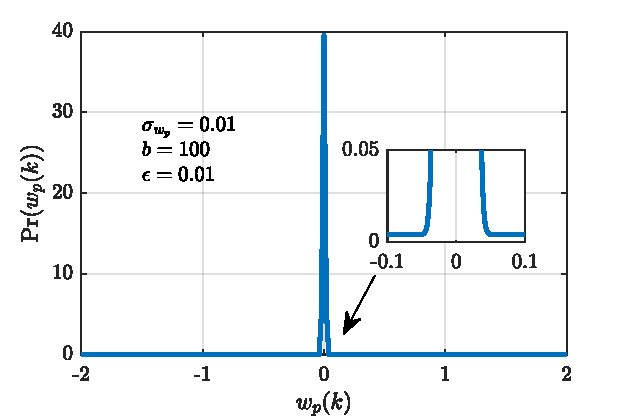
\includegraphics[width=11.5cm]{wpk-pdf-4.pdf}
	\caption{Probability density of a random shock signal}
	\label{fig:wpk-pdf}
\end{figure}

When dealing with a system having more than one \gls{RODD}, where each random shock is independent, the notation is
\begin{equation} \label{eq:wpik2}
	w_{p,i}(k) \sim 
	\begin{cases*}
		\mathcal{N}\left(0, \sigma_{w_p,i}^2\right) & with probability $1-\varepsilon_i$, \\
		\mathcal{N}\left(0, b_i^2\sigma_{w_p,i}^2\right) & with probability $\varepsilon_i$,
	\end{cases*}
\end{equation}
where $i \in \left\{1, 2, ..., n_p\right\}$.
\nomenclature{$n_p$}{number of independent random shock disturbance processes}%

The choice of $A(q^{-1})$ and $B(q^{-1})$ in \eqref{eq:RODD} determines the nature of the \gls{RODD}. For example, if $B(q^{-1})=1$ and $A(q^{-1})=1-q^{-1}$, $p(k)$ will be a random-walk process with infrequent, large step changes.

% Add symbol to glossary
Using $\nabla$ to denote $1-q^{-1}$, the \gls{RODD} \textit{step-disturbance} process can be defined as
\nomenclature{$\nabla$}{defined as $1-q^{-1}$}%
\begin{equation} \label{eq:RODD-step}
	p(k) = \frac{1}{\nabla}w_p(k).
\end{equation}

A \gls{RODD} \textit{ramp-disturbance}, consisting of a series of ramps with randomly-occurring changes in slope, may be generated using
\begin{equation} \label{eq:RODD-ramp}
	p(k) = \frac{1}{\nabla^2}w_p(k).
\end{equation}

A \gls{RODD} consisting of randomly-occurring decaying exponential changes may be generated using
\begin{equation} \label{eq:RODD-exp}
	p(k) = \frac{1}{(1-a_1q^{-1})\nabla}w_p(k),
\end{equation}
where  $0<a_1<1$. Note that $a_1=0$ corresponds to the case of a \gls{RODD} step disturbance \eqref{eq:RODD-step} and $a_1=1$ to that of a \gls{RODD} ramp disturbance \eqref{eq:RODD-ramp}. 

An equivalent state-space representation of \eqref{eq:RODD-exp} is
\begin{equation} \label{eq:RODD-ss}
	\begin{split}
		\mathbf{x}_p(k+1) & =\left[\begin{array}{cc}
			1 & 1 \\
			0 & a_1
		\end{array}\right] \mathbf{x}_p(k) +\left[\begin{array}{cc}
			0 \\
			1
		\end{array}\right] w_p(k) \\
		p(k) & =\left[\begin{array}{cc}
			1 & 0
		\end{array}\right] \mathbf{x}_p(k),
	\end{split}
\end{equation}
\nomenclature{$\mathbf{x}_p(k)$}{disturbance model states at time $k$}%
where $\mathbf{x}_p(k) \in \mathbb{R}^2$ is the state vector.

A disturbance with a combination of different \gls{RODD}s is also possible.  For example, a state-space representation of a \gls{RODD} consisting of step changes and ramps is
\begin{equation} \label{eq:RODD-step-ramp}
	\begin{split}
		\mathbf{x}_p(k+1) & =\left[\begin{array}{cc}
			1 & 1 \\
			0 & 1
		\end{array}\right] \mathbf{x}_p(k) +\left[\begin{array}{cc}
			1 & 0 \\
			0 & 1
		\end{array}\right] \mathbf{w}_p(k) \\
		p(k) & =\left[\begin{array}{cc}
			1 & 0
		\end{array}\right] \mathbf{x}_p(k),
	\end{split}
\end{equation}

where $\mathbf{w}_p(k)$ is a vector of two independent random shock signals generated by \eqref{eq:wpik2}. Simulated examples of these \gls{RODD}s are presented in figures \ref{fig:rodd-sim-plots} and \ref{fig:rodd-sim-plot2}.

\subsection{Hidden Markov models} \label{sec:HMM}

\textit{Hidden Markov models} (\gls{HMM}) can be used to simulate a more diverse set of switching behaviours than those of the \gls{RODD} model described in the previous section \citep{wong_realistic_2009}. A Markov process or Markov chain is a stochastic model used to describe a sequence of discrete events for which the probability of future events depends only on the current state. A \gls{HMM} is a Markov model with states that are not fully observable (i.e. hidden or observed with a measurement error).

To illustrate the basic concept, the state of the random shock process \eqref{eq:wpk2} \hl{may be defined} as a Markov model with a state that has two possible values,
\begin{equation} \label{eq:gamma-k}
	\gamma(k) \in \{0,1\}.
\end{equation}
\nomenclature{$\gamma(k)$}{random shock indicator at time $k$}%
$\gamma(k)=1$ represents a shock at time $k$, and $\gamma(k)=0$ means no shock occurs. The switching of $\gamma(k)$ can then be defined by a \textit{transition matrix}, $\Pi$, which describes the probabilities of transitioning from every mode at time $k$ to every mode at time $k+1$:
\begin{equation} \label{eq:Pi}
	\begin{aligned}
	\Pi &= \left(\pi_{ij} \forall i,j\in \{1,2,...,n_j\}\right) \\
	\pi_{ij} &= \Pr\left( \gamma(k)=j-1 \mid \gamma(k-1)=i-1 \right),
	\end{aligned}
\end{equation}
\nomenclature{$\Pr(A \mid B)$}{probability of an event $A$ given an event $B$}%
\nomenclature{$n_j$}{number of modes or models of a switching system}%
where $n_j$ is the number of possible system modes and $\pi_{ij}$ is the probability that the system mode at time $k$ is $j-1$ given that it was $i-1$ at time $k-1$.

In the case of the random shock, $n_j=2$ and the equivalent Markov process has the transition probability matrix
\nomenclature{$\Pi_{w_{p}}$}{transition probability matrix of the disturbance process $w_p$}%
\begin{equation} \label{eq:Pi-RODD-step}
	\Pi_{w_{p}} = \begin{bmatrix}
	1-\varepsilon & \varepsilon \\
	1-\varepsilon & \varepsilon
	\end{bmatrix}.
\end{equation}
Since $w_{p}(k)$ is an independent random variable, it does not depend on the previous state, $\gamma(k-1)$. Therefore, the rows of $\Pi_{w_{p}}$ are identical.

The use of the Markov model thus allows transition probabilities that do depend on the previous state. For example, consider a disturbance where the signal switches infrequently between samples from two or more distributions with different parameters. The probabilities of switching from one distribution to another may be different. Such a disturbance process could be simulated with a hidden Markov model by conditioning the distribution from which $w_p(k)$ is sampled on a Markov state, $r(k)$, with an arbitrary number of modes,
\nomenclature{$r(k)$}{mode indicator of a switching system at time $k$}%
\begin{equation} \label{eq:mog-example}
	\begin{split}
		w_p(k) \sim 
		\begin{cases*}
			\mathcal{N}\left(\mu_{w_p,1}, \sigma_{w_p,1}\right) & if $r(k)=1$, \\
			\mathcal{N}\left(\mu_{w_p,2}, \sigma_{w_p,2}\right) & if $r(k)=2$, \\
			... & ...\\
			\mathcal{N}\left(\mu_{w_p,n_j}, \sigma_{w_p,n_j}\right) & if $r(k)=n_j$.
		\end{cases*} \\
	\Pr(r(k)=j-1 \mid r(k-1)=i-1)=\pi_{ij} \forall i,j \in {1,2,...,n_j}
	\end{split}
\end{equation}

To make the notation more concise, allow the value of any time-varying discrete variable such as $\sigma_{w_p} \in \left\{\sigma_{w_p,1}, \sigma_{w_p,2},..., \sigma_{w_p,n_j}\right\}$, to be determined by the value of the Markov state $r(k)$. Thus,
\begin{equation} \label{eq:A-selection}
	\sigma_{w_p}(r(k)) = 
	\begin{cases*}
		\sigma_{w_p,1} & if $r(k)=1$, \\
		\sigma_{w_p,2} & if $r(k)=2$, \\
		... & ...\\
		\sigma_{w_p,n_j} & if $r(k)=n_j$.
	\end{cases*}
\end{equation}

With this notation, \eqref{eq:mog-example} can be written concisely as
\begin{equation} \label{eq:mog-example2}
	\begin{aligned}
		w_p(k) &\sim \mathcal{N}\left(\mu_{w_p}(r(k)), \sigma_{w_p}(r(k))\right) \\
		\Pr(r(k) &= j-1 \mid r(k-1)=i-1)=\pi_{ij} \forall i,j \in {1,2,...,n_j}.
	\end{aligned}
\end{equation}
where $\mu_{w_p}\in\left\{\mu_{w_p,1},\mu_{w_p,2},...,\mu_{w_p,n_j}\right\}$. This model is known as a \textit{mixture of Gaussians} and can be considered a special-case of a HMM-based disturbance model \citep{wong_disturbance_2007}.

A \gls{HMM} disturbance process can be represented by a \textit{Markov jump linear system} (\acrshort{MJLS}) \citep{costa_discrete-time_2005}. The state-space representation with time-varying system matrices $\mathbf{A}(\gamma(k))$, $\mathbf{B}(\gamma(k))$, and $\mathbf{C}(\gamma(k))$, and a vector of independent time-varying random shock inputs, $\mathbf{w}_p(k)$ \eqref{eq:mog-example2}, is defined
\begin{equation} \label{eq:MJLS}
	\begin{aligned}
	\mathbf{x}_p(k+1) &= \mathbf{A}(r(k)) \mathbf{x}_p(k) + \mathbf{B}(r(k))\mathbf{w}_p(k) \\
	\mathbf{p}(k) &= \mathbf{C}(r(k)) \mathbf{x}_p(k) + \mathbf{e}_p(k).
	\end{aligned}
\end{equation}

Note that $\mathbf{e}_p(k)$ may also be a switching random variable if desired. \eqref{eq:MJLS} is a versatile model suitable for representing and simulating a diverse family of stochastic disturbances.

\subsection{Bounded disturbances} \label{sec:bounded}

The \textit{bounded random walk} (\gls{BRW}) is a stochastic process proposed by \cite{nicolau_stationary_2002}. The discrete-time version is defined by the difference equation
\begin{equation} \label{eq:brw}
		p(k+1) = p(k) + a(p(k)) + e(k),
\end{equation}
where $e(k)$ is a random noise with variance $\sigma_e^2$, and $a(\cdot)$ is a function defined as
\nomenclature{$a(\cdot)$}{additive bias function used in the \acrshort{BRW}}%
\nomenclature{$\alpha_{1}$}{\acrshort{BRW} parameter}%
\nomenclature{$\alpha_{2}$}{\acrshort{BRW} parameter}%
\nomenclature{$\tau$}{\acrshort{BRW} parameter}%
\begin{equation}
	a(x) = e^{\beta}\left(e^{-\alpha_{1}\left(x - \tau\right)} - e^{\alpha_{2}\left(x - \tau\right)}\right),
\end{equation}
where $\beta$, $\alpha_{1}$, and $\alpha_{2}$ are constants.  From \eqref{eq:brw} it can be deduced that
\begin{equation}
	\mathbb{E}\{p(k+1)|p(k)\} = p(k) + a(p(k)).
\end{equation}

Therefore, $a(p(k))$ has the effect of an additive bias or time-varying adjustment to $p(k+1)$ that depends on $p(k)$. The shape of $a(\cdot)$ is determined by the constants $\alpha_{1}$,  $\alpha_{2}$, $\beta$, and $\tau$. Figure \ref{fig:brw-a} shows $a(p(k))$ in the case where $\tau=100$, $\beta=-15$, and $\alpha_{1}=\alpha_{2}=3$.  From this, it is clear that in the vicinity of $p(k)=\tau$, $a(p(k))\approx0$. When $a(p(k))=0$, \eqref{eq:brw} is the equation for a random walk. However, outside the neighbourhood, $p(k) \approx \tau$, $a(p(k))$ increases for low $p(k)$ or decreases for high $p(k)$. This has the effect of causing $p(k+1)$ to revert towards the mean ($\tau$) whenever $p(k)$ strays outside the neighbourhood. 
\begin{figure}[ht]
	\centering
	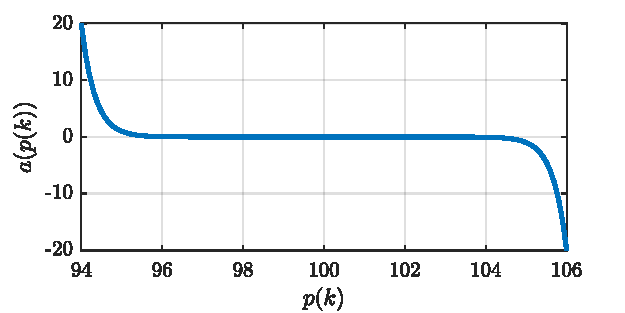
\includegraphics[height=5cm]{images/brw_a.pdf}
	\caption{A bounded random walk bias function}
	\label{fig:brw-a}
\end{figure}

Figure \ref{fig:brw-sim} shows a simulation of a \gls{BRW} with the above parameter values, and for comparison, an unbounded random walk (labelled `RW') generated with the same noise input. The dashed lines at $p(k)=95$ and $p(k)=105$ roughly indicate the location of the lower and upper bounds, which the \gls{BRW} only marginally exceeds.
\begin{figure}[ht]
	\centering
	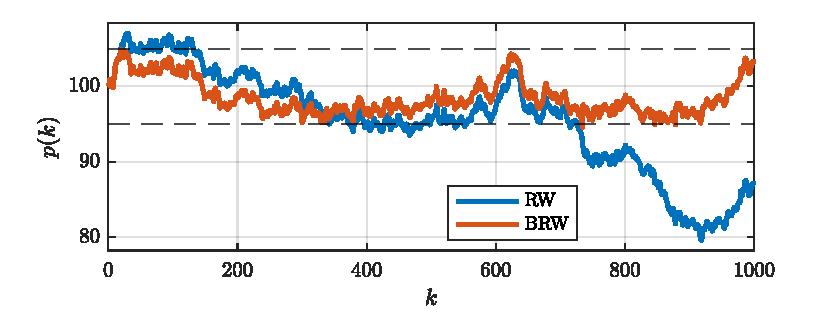
\includegraphics[height=5cm]{images/brw_sim.pdf}
	\caption{Examples of a bounded and unbounded random walk}
	\label{fig:brw-sim}
\end{figure}

Unlike a simple random walk, the \gls{BRW} is stationary. \cite{nicolau_stationary_2002} derived a formula for the form of the unconditional (i.e. stationary) probability distribution of the continuous-time \gls{BRW}. Figure \ref{fig:brw-pdf} shows the normalized stationary probability density of the \gls{BRW} defined above. For comparison, the probability density of a random walk process after 20 sample periods is also shown. It can be seen that there is a significant probability that the random walk would exceed the bounds of this \gls{BRW} after 20 sample periods. It can also be seen that the central part of the probability distribution of the \gls{BRW} is flat, indicating that all values within the bounds are equally likely after a large number of samples, similar to a uniform probability distribution.

%\begin{equation}
%	p_{BRW}(x) \propto \sigma^{-2} \exp \left\{-\frac{2 e^{k}}{\sigma^{2}}\left(\frac{e^{-\alpha_{1}(x-\tau)}}{\alpha_{1}}+\frac{e^{\alpha_{2}(x-\tau)}}{\alpha_{2}}\right)\right\}
%\end{equation}

\begin{figure}[ht]
	\centering
	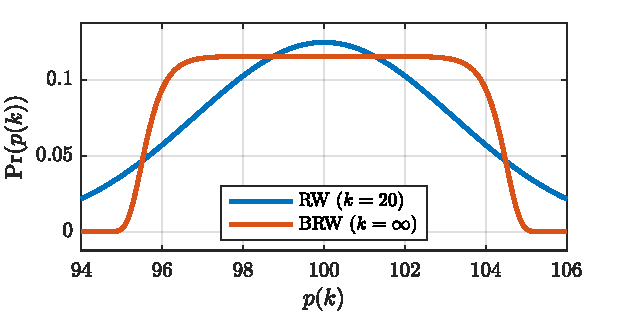
\includegraphics[height=5cm]{images/brw_pdf.pdf}
	\caption{Probability distributions of bounded and unbounded random walks}
	\label{fig:brw-pdf}
\end{figure}

However, the \gls{BRW} as defined in \eqref{eq:brw} is not guaranteed to be stable. Extreme values of $p(k)$ may cause $|a(p(k))|$ to be greater than $2|p(k)|$, which results in rapid divergence. This would cause computational errors in a numerical simulation. To avoid this, \cite{nicolau_stationary_2002} recommends adding a conditional regularizing step that forces reversion towards the mean, $\tau$, when the correction bias is too large. Instead of \eqref{eq:brw}, a conditional difference equation,
\begin{equation} \label{eq:brw-reg}
	p(k+1) = \begin{cases*}
		p(k) + a(p(k)) + e(k) & if $\left|a(p(k)) \right| < 2\left| p(k) - \tau \right|$, \\
		\tau + \phi(p(k) - \tau) + e(k) & if $\left|a(p(k)) \right| \geq 2\left| p(k) - \tau \right|$,
	\end{cases*}
\end{equation}
is used, where $\phi$ is a constant such that $0<\phi<1$. The size of $\phi$ determines how fast $p(k)$ reverts to $\tau$ when it is outside the stable region.

Since the \gls{BRW} has a non-Gaussian probability distribution, analysis of the properties of any dynamical system with a \gls{BRW} input is difficult. However, for simulation purposes, the \gls{BRW} is a simple and practical solution to the problem of bounding a random disturbance.

The \gls{BRW} concept could be extended to \gls{RODD}s. A \gls{RODD} step disturbance \eqref{eq:RODD-step} is a random walk with a switching noise variance \eqref{eq:wpk2}. The concern when trying to bound such a disturbance is the large step changes that occur infrequently. Since the probability of the shock, as well as the sign and amplitude of the step, are independent random variables, a \gls{RODD} step disturbance that happens to be at one of the bounds is as likely to step outside the bound as it is to step back inside the bounded region. The conditional regularity used in the \gls{BRW} \eqref{eq:brw-reg} would prevent any computational problems.


\section{State estimation} \label{sec:estimation}

State estimation is the task of estimating the values of the state variables of a dynamic model of a system given a set of measurements from the system. In process control applications, estimates of the states at the current time, or a prediction of their values at the next time instant, are required in real time (i.e. online) in order to calculate an appropriate control action.

Consider the diagram of an input-output system model in Figure \ref{fig:model_diag_uwvy}. Here, $\mathbf{u}(k)$ $\in \mathbb{R}^{n_u}$ is a vector of known input variables at time instant $k$, $\mathbf{w}(k)$ $\in \mathbb{R}^n$ is a vector of unmeasured state disturbances, $\mathbf{v}(k) \in \mathbb{R}^{n_y}$ is a vector of measurement errors, and $\mathbf{y}_M(k) \in \mathbb{R}^{n_y}$ is a vector of output measurements. The box represents a mathematical model that relates the inputs to the outputs and may be time-varying.
\nomenclature{$\mathbf{u}(k)$}{system inputs at time $k$}%
\nomenclature{$\mathbf{y}(k)$}{system outputs at time $k$}%
\nomenclature{$\mathbf{w}(k)$}{process disturbances at time $k$}%
\nomenclature{$\mathbf{v}(k)$}{measurement noises at time $k$}%
\begin{figure}[ht]
	\centering
	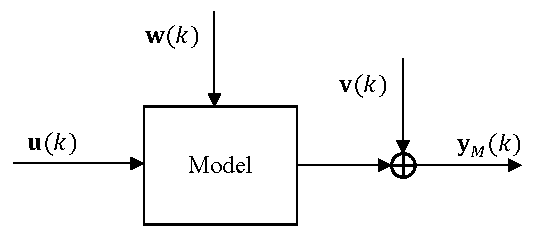
\includegraphics[width=8cm]{images/model_diag_uwvy.pdf}
	\caption{System model diagram}
	\label{fig:model_diag_uwvy}
\end{figure}

A convenient form in which to represent discrete-time, linear, possibly time-varying, dynamical system models for state estimation and control purposes, is the state-space representation
\begin{equation} \label{eq:ss_rep_uwy}
	\begin{aligned}
		\mathbf{x}(k+1) &= \mathbf{A}(k) \mathbf{x}(k) + \mathbf{B}(k) \mathbf{u}(k) + \mathbf{w}(k), \\
		\mathbf{y}_M(k) &= \mathbf{C}(k) \mathbf{x}(k) + \mathbf{v}(k).
	\end{aligned}
\end{equation}
\nomenclature{$\mathbf{x}(k)$}{system model states at time $k$}%
\nomenclature{$\mathbf{A}$}{transition matrix of the system model}%
\nomenclature{$\mathbf{B}$}{input matrix of the system model}%
\nomenclature{$\mathbf{C}$}{output matrix of the system model}%
where $\mathbf{x}(k)$ $\in \mathbb{R}^n$ is a vector of state variables, $\mathbf{A}(k) \in \mathbb{R}^{n \times n}$ is the state transition matrix at time $k$, $\mathbf{B}(k) \in \mathbb{R}^{n \times n_u}$ is the input matrix at time $k$, and $\mathbf{C}(k) \in \mathbb{R}^{n_y \times n}$ is the output matrix at time $k$. In this work, the system matrices are not time-varying and are therefore denoted $\mathbf{A}$, $\mathbf{B}$, and $\mathbf{C}$ in the remainder of this chapter.

The \textit{Kalman filter} \citep{kalman_new_1960} is the optimal estimator for a linear system in which the unmeasured disturbances and measurement errors are Gaussian random variables with mean values of zero. There are two commonly-used implementations of the Kalman filter, the \textit{prediction form} and the \textit{filtering form}. In the prediction form, the estimates of the states at the next time instant ($k+1$), given the information available at the current time ($k$) are calculated using
\begin{equation}
\begin{aligned} \label{eq:xkp1_hat_p}
	\mathbf{\hat{x}}(k+1 \mid k) &= \mathbf{\hat{x}}(k+1 \mid k-1) + \mathbf{K}_p(k) \big( \mathbf{y}_M(k) - \mathbf{\hat{y}}(k \mid k-1) \big) \\
	&= \mathbf{A}\mathbf{\hat{x}}(k \mid k-1) + \mathbf{B}\mathbf{u}(k) + \mathbf{K}_p(k) \big( \mathbf{y}_M(k) - \mathbf{C} \mathbf{\hat{x}}(k \mid k-1) \big)
\end{aligned}
\end{equation}
\nomenclature{$\mathbf{y}_M(k)$}{system output measurements at time $k$}%
where $\hat{\mathbf{x}}(k \mid k-1)$ is the prediction of the states at time $k$ that was made with the information available at the previous time instant, $k-1$, $\mathbf{y}_M(k)$ is the current measurement of the output, and $\mathbf{K}_p(k) \in \mathbb{R}^{n \times n_y}$ is a (possibly time-varying) correction gain.
\nomenclature{$\mathbf{K}_p(k)$}{correction gain of the Kalman filter (prediction form)}%

In the filtering form, which is used in this work, the estimated states and outputs at the current time are calculated given the information available at the current time using
\begin{equation} \label{eq:xkyk_hat}
	\begin{aligned}
		\mathbf{\hat{y}}(k \mid k-1) &= \mathbf{C} \mathbf{\hat{x}}(k \mid k-1) \\
		\mathbf{\hat{x}}(k \mid k) &= \mathbf{\hat{x}}(k \mid k-1) + \mathbf{K}(k) \big( \mathbf{y}_M(k) - \mathbf{\hat{y}}(k \mid k-1)  \big) \\
		\mathbf{\hat{y}}(k \mid k) &= \mathbf{C} \mathbf{\hat{x}}(k \mid k)
	\end{aligned}
\end{equation}
\nomenclature{$\hat{\mathbf{x}}(k \mid k-1)$}{predictions of system model states at time $k$ made with information available at time $k-1$}%
\nomenclature{$\mathbf{K}(k)$}{correction gain of the Kalman filter (filtering form)}%
where $\mathbf{K}(k)$ $\in \mathbb{R}^{n \times n_y}$ is a (possibly time-varying) correction gain. Instead of \eqref{eq:xkp1_hat_p}, the predictions of the states at the next time instant are calculated using
\nomenclature{$\hat{\mathbf{x}}(k+1 \mid k)$}{predictions of system modelstates at time $k+1$ made with information available at time $k$}%
\nomenclature{$\hat{\mathbf{x}}(k \mid k)$}{estimates of system model states at time $k$ made with information available at time $k$}%
\nomenclature{$\hat{\mathbf{y}}(k \mid k)$}{estimates of system outputs at time $k$ made with information available at time $k$}%
\begin{equation} \label{eq:xkp1_hat}
	\mathbf{\hat{x}}(k+1 \mid k) = \mathbf{A} \mathbf{\hat{x}}(k \mid k) + \mathbf{B} \mathbf{u}(k).
\end{equation}

An intuitive interpretation of the Kalman filter is that it takes the predictions of the states at time $k$ made in the previous time instant using the system model, and corrects them based on the difference between the current output measurement, $\mathbf{y}_M(k)$, and the output predicted by the model, $\mathbf{C} \mathbf{\hat{x}}(k \mid k-1)$. The correction step \eqref{eq:xkyk_hat} and prediction step \eqref{eq:xkp1_hat} are executed iteratively each time step, given a prior prediction of the states at time zero, $\mathbf{\hat{x}}(0 \mid -1)=\mathbf{\hat{x}}_0$.
\nomenclature{$\mathbf{\hat{x}}_0$}{Initial values of the estimates of the system states at time 0}%

Although the predicted states, $\hat{\mathbf{x}}(k \mid k-1)$, are identical in both forms of the Kalman filter, the use of the updated (i.e. \textit{a posteriori}) estimates, $\hat{\mathbf{x}}(k \mid k)$, in the filtering form instead of the predicted states leads to an optimal estimate taking account of all the information available. However, it should be noted that in some control applications, the prediction form is beneficial because the state predictions, $\hat{\mathbf{x}}(k+1 \mid k)$, are available one time step ahead.

To track a system with time-varying parameters, a dynamic estimator is needed with a time-varying correction gain. In the case of the filtering form of the Kalman filter, $\mathbf{K}(k)$ is calculated at each time instant using
\begin{equation} \label{eq:Kk}
	\mathbf{K}(k) = \mathbf{P}(k \mid k-1)\mathbf{C}^\intercal \mathbf{S}^{-1}(k),
\end{equation}
where $\mathbf{S}(k)$ is the output prediction error covariance matrix, which is given by
\nomenclature{$\mathbf{S}(k)$}{covariance of the output prediction errors at time $k$}%
\begin{equation} \label{eq:Sk}
	\mathbf{S}(k) = \mathbf{C}\mathbf{P}(k \mid k-1)\mathbf{C}^\intercal + \mathbf{R},
\end{equation}
\nomenclature{$\mathbf{P}(k \mid k-1)$}{predictions of the state estimation error covariance at time $k$ made with information available at time $k-1$}%
and $\mathbf{P}(k \mid k-1)$ is the state estimation error covariance matrix calculated in the previous time instant. $\mathbf{R}$, which is time invariant in this work, is the covariance matrix of the measurement noises,
\nomenclature{$\mathbf{R}$}{covariance of the measurement noises in the observer model}%
\begin{equation} \label{eq:R}
	 \mathbf{R} = \mathbb{E}\{ \mathbf{v}(k) \mathbf{v}^\intercal(k) \},
\end{equation}
\nomenclature{$\mathbb{E}\{\cdot\}$}{expectation operator}%
where $\mathbb{E}\{\cdot\}$ is the expectation operator.

The corrected error covariance may be calculated using
\nomenclature{$\mathbf{P}(k \mid k)$}{state estimation error covariance at time $k$ made with information available at time $k$}%
\begin{equation} \label{eq:Pk}
	\mathbf{P}(k \mid k) = \left( \mathbf{I}_n - \mathbf{K}(k) \mathbf{C} \right) \mathbf{P}(k \mid k-1),
\end{equation}
given an initial covariance estimate at time zero, $\mathbf{P}(0 \mid -1)=\mathbf{P}_0$.%
\nomenclature{$\mathbf{P}_0$}{Initial value of the state estimation error covariance at time 0}

However, to reduce numerical errors due to rounding, the computation of $\mathbf{P}(k \mid k)$ is carried out in this work using the Joseph stabilized version of \eqref{eq:Pk} {\citep{lewis_optimal_2008}
 \begin{equation} \label{eq:Pk-stab}
 	\mathbf{P}(k \mid k) = \left( \mathbf{I}_n - \mathbf{K}(k) \mathbf{C} \right ) \mathbf{P}(k \mid k-1) \left( \mathbf{I}_n - \mathbf{K}(k) \mathbf{C} \right )^\intercal + \mathbf{K}(k)  \mathbf{R} \mathbf{K}(k)^\intercal,
 \end{equation}
\nomenclature{$\mathbf{I}_n$}{the identity matrix ($n \times n$)}%
where $\mathbf{I}_n$ is the identity matrix.

The prediction of the error covariance at the next time instant is made using
\nomenclature{$\mathbf{P}(k+1 \mid k)$}{predictions of the state estimation error covariance at time $k+1$ made with information available at time $k$}%
\begin{equation} \label{eq:Pkp1}
	\mathbf{P}(k+1 \mid k) = \mathbf{A} \mathbf{P}(k \mid k)  \mathbf{A}^\intercal  + \mathbf{Q}(k),
\end{equation}
where $\mathbf{Q}(k)$ is the time-varying covariance of the process disturbances,
\nomenclature{$\mathbf{Q}(k)$}{covariance of the process disturbances in the observer model at time $k$}%
\begin{equation} \label{eq:Q}
	\mathbf{Q}(k) = \mathbb{E}\{ \mathbf{w}(k) \mathbf{w}^\intercal(k) \}.
\end{equation}

Algorithm \ref{alg:kf} defines the sequence of the Kalman filter calculations at each time instant. 
\nomenclature{$\mathcal{Q}$}{set of process noise covariance matrices of a switching system model}%
This is for the case with only the covariance, $\mathbf{Q}(k)$, switching according to the shock indicator, $\gamma(k)$, \eqref{eq:init_Q}. It can easily be extended to simulate other switching model components, such as $\mathbf{R}(k)$, $\mathbf{A}(k)$, $\mathbf{B}(k)$, or $\mathbf{C}(k)$ as defined in \eqref{eq:ss_rep_uwy}. \hl{An alternative to the representation used in this work would be to implement the switching of the random shock {\eqref{eq:wpk2}} using a time-varying input matrix, $\mathbf{B}(k)$, instead of the time-varying prediction error covariance, $\mathbf{Q}(k)$ in {\eqref{eq:Pkp1}}. Both methods are valid and equivalent.}
\begin{algorithm}
	\caption{Kalman filter update}\label{alg:kf}
	%\algorithmfootnote{$y_0$ denotes the initial value.}
	\begin{algorithmic}
		\Require $\mathbf{A},\mathbf{B},\mathbf{C},\mathbf{\hat{x}}(k \mid k-1), \mathbf{P}(k \mid k-1), \mathcal{Q}, \mathbf{R}, \mathbf{\gamma}(k), \mathbf{u}(k), \mathbf{y}_M(k)$
		\State calculate $\mathbf{S}(k)$ \eqref{eq:Sk}
		\State calculate $\mathbf{K}(k)$ \eqref{eq:Kk}
		\State calculate $\mathbf{\hat{x}}(k \mid k)$ and $\mathbf{\hat{y}}(k \mid k)$ \eqref{eq:xkyk_hat}
		\State calculate $\mathbf{P}(k \mid k)$ \eqref{eq:Pk-stab}
		\State calculate $\mathbf{\hat{x}}(k+1 \mid k)$ \eqref{eq:xkp1_hat}
		\State $\mathbf{Q}(k) \gets \mathcal{Q}(\gamma(k))$
		\State calculate $\mathbf{P}(k+1 \mid k)$ \eqref{eq:Pkp1}
	\end{algorithmic}
\end{algorithm}

Also note that in a control application, the manipulated input, $\mathbf{u}(k)$, is computed by the control algorithm. This may be done before the Kalman filter calculations in algorithm \ref{alg:kf} if the prior prediction of the states in the current time instant, $\hat{\mathbf{x}}(k \mid k-1)$, is used. Alternatively, slightly better control performance might be achieved if the control algorithm uses the updated (a-posteriori) state estimates, $\hat{\mathbf{x}}(k \mid k)$. In the latter case, the Kalman filter calculations must be interrupted to compute the control action after the state correction step \eqref{eq:xkyk_hat} and prior to the prediction step \eqref{eq:xkp1_hat}, when $\mathbf{u}(k)$ is needed.

\begin{figure}[ht]
	\centering
	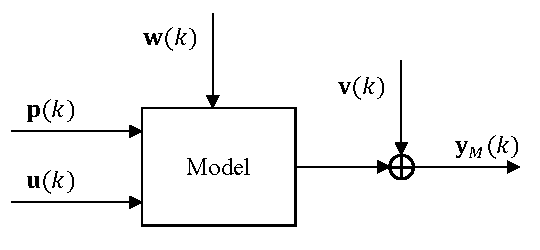
\includegraphics[width=8cm]{images/model_diag_upwvy.pdf}
	\caption{System model with disturbance inputs and manipulated inputs}
	\label{fig:model_diag_upwvy}
\end{figure}
In the case where the system has unmeasured disturbance inputs, $\mathbf{p}(k) \in \mathbb{R}^{n_p}$, as depicted in Figure \ref{fig:model_diag_upwvy}, the state-space equations \eqref{eq:ss_rep_uwy} are modified to include these by splitting the input matrix into two parts, $\mathbf{B}_u \in \mathbb{R}^{n \times n_u}$ and $\mathbf{B}_p \in \mathbb{R}^{n \times n_p}$,
\begin{equation} \label{eq:ss_rep_upwy}
	\begin{aligned}
		\mathbf{x}(k+1) = \mathbf{A} \mathbf{x}(k) + \mathbf{B}_u \mathbf{u}(k) + \mathbf{B}_p \mathbf{p}(k) + \mathbf{w}(k), \\
		\mathbf{y}_M(k) = \mathbf{C} \mathbf{x}(k) + \mathbf{v}(k).
	\end{aligned}
\end{equation}

For state estimation in the presence of unmeasured disturbances, which is always the case in practice, a suitable model of the disturbances is needed. This model is shown in Figure \ref{fig:model_diag_wpupwvy} with a vector of random shock variables, $\mathbf{w}_p(k)$, at its input.
\nomenclature{$\mathbf{w}_p(k)$}{random shock signals at time $k$}%
\begin{figure}[ht]
	\centering
	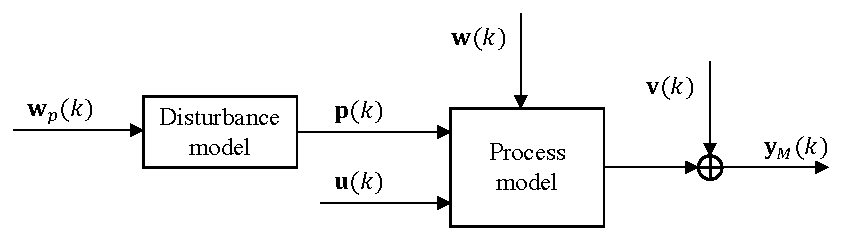
\includegraphics[width=12.5cm]{images/model_diag_wpupwvy.pdf}
	\caption{System with process model and disturbance model}
	\label{fig:model_diag_wpupwvy}
\end{figure}

A state-space representation of the combined system including the disturbance model can be constructed. This is referred to as the \textit{augmented system model},
\begin{equation} \label{eq:ss_rep_xa}
	\begin{aligned}
		\mathbf{x}_a(k+1) = \mathbf{A}_a \mathbf{x}_a(k) + \mathbf{B}_{a,u} \mathbf{u}(k) + \mathbf{B}_{a,w} \mathbf{w}_{a}(k), \\
		\mathbf{y}(k) = \mathbf{C}_a \mathbf{x}_a(k) + \mathbf{v}(k),
	\end{aligned}
\end{equation}
%\nomenclature{$\mathbf{x}_a(k)$}{augmented system states at time $k$}%
where $\mathbf{x}_a(k) \in \mathbb{R}^{n+n_p}$ is an augmented state vector that includes the states of both the process model and the disturbance model, 
\begin{equation} \label{eq:xak}
	\mathbf{x}_a(k) = \begin{bmatrix}
		\mathbf{x}(k) \\
		\mathbf{x}_p(k)
	\end{bmatrix},
\end{equation}
and $\mathbf{w}_a(k) \in \mathbb{R}^{n+n_p}$ is an augmented vector of random variables, including the random shocks,
\begin{equation} \label{eq:wak}
	\mathbf{w}_a(k) = \begin{bmatrix}
		\mathbf{w}(k) \\
		\mathbf{w}_p(k)
	\end{bmatrix}.
\end{equation}

However, note that this notation with subscript `a' is only used in this section. In subsequent sections, the subscript is dropped for simplicity since all references to the system model refer to the augmented model used for state estimation.

Although the random shock in a \gls{RODD} is unmeasured, it may be observable from the measurements of the outputs of the system. As mentioned in Section \ref{detection_RODDs}, systems with \gls{RODD}s pose problems for state estimation using standard Kalman filters due to the switching of the noise model parameters, namely, the variance of $w_p(k)$ \eqref{eq:wpk2}. As explained by \cite{andersson_adaptive_1985}, a trade-off must be made during the filter design between its ability to respond to the infrequent disturbance when it occurs, and its sensitivity to noise at other times.


\subsection{Multiple model approaches} \label{sec:multi-model}

One option for state estimation of switching (i.e. hybrid) systems is the so-called \textit{multiple-model approach}. Multiple-model observers account for different possible hypotheses about the current and past states of the system and infer from these an overall `best' estimate of the current states. To achieve this, an independent Kalman filter is maintained for each hypothesis and a weighted average of the estimates by each filter is calculated using the conditional probabilities of each hypothesis given current and past measurements.

Let the number of hypotheses and Kalman filters be $n_h$ and the \textit{shock mode hypothesis} associated with Kalman filter $f$ at time $k$ be
\nomenclature{$n_h$}{number of hypotheses maintained by a multiple-model observer}%
\begin{equation} \label{eq:gammak}
	\gamma_{f}(k) \in \left\{0, 1 \right\} \forall{k \ge 0}.
\end{equation}

First, consider the case of estimating only one shock signal \eqref{eq:wpk2}. Therefore, $\gamma_f(k)$ is a scalar. The transition probabilities of the random shock are independent of previous shocks:
\nomenclature{$\gamma_f(k)$}{random shock indicator of hypothesis $f$ at time $k$}%
\begin{equation} \label{eq:Pr_gammak_given_gammakm1}
	\begin{aligned}
		& \Pr\left(\gamma_{f}(k)=0 \mid \gamma_{f}(k-1)\right) = \Pr\left(\gamma_{f}(k)=0\right) = 1-\varepsilon, \\
		& \Pr\left(\gamma_{f}(k)=1 \mid \gamma_{f}(k-1)\right) = \Pr\left(\gamma_{f}(k)=1\right) = \varepsilon.
	\end{aligned}
\end{equation}

After $k$ time steps, the complete shock mode hypothesis sequence associated with filter $f$ is
\nomenclature{$\Gamma_f(k)$}{shock indicator hypotheses sequence $f$ from time $0$ to $k$}%
\begin{equation} \label{eq:Gammak}
	\Gamma_f(k) = \left\{ \gamma_f(0), \gamma_f(1), ..., \gamma_f(k) \right\}.
\end{equation}

The known system inputs and output measurements up to time $k$ are
\nomenclature{$\mathbf{U}(k)$}{known system inputs from time 0 to time $k$}%
\nomenclature{$\mathbf{Y}(k)$}{system outputs from time 0 to time $k$}%
\nomenclature{$\mathbf{Y}_M(k)$}{system output measurements from time 0 to time $k$}%
\begin{equation} \label{eq:Uk_Yk}
	\begin{aligned}
		\mathbf{U}(k) = \left\{ \mathbf{u}(0), \mathbf{u}(1), ..., \mathbf{u}(k) \right\} \\
		\mathbf{Y}_M(k) = \left\{ \mathbf{y}_M(0), \mathbf{y}_M(1), ..., \mathbf{y}_M(k) \right\}.
	\end{aligned}
\end{equation}

Assume that new measurements are made available at each time $k$. The probability of the shock hypothesis sequences associated with each filter given the data up to time $k$ can be calculated recursively using the following equations. At time $k$, the probability of the shock hypothesis sequence associated with filter $f$ given the data up to time $k-1$ is
\begin{multline} \label{eq:Pr_Gammak_given_Ykm1}
	\Pr(\Gamma_f(k) \mid \mathbf{Y}_M(k-1)) = 
	\Pr(\gamma_f(k) \mid \gamma_f(k-1)) \Pr(\Gamma_f(k-1) \mid \mathbf{Y}_M(k-1)).
\end{multline}

The conditional probability densities of the measurements, $\mathbf{y}_M(k)$, are approximated by Gaussian distributions centred on the output predictions, $\mathbf{\hat{y}}_{f}(k \mid k-1)$,  and with the variance of the output prediction error, $\mathbf{S}_f(k)$,
\begin{equation} \label{eq:p_yk_given_Gammak_Ykm1}
	p(\mathbf{y}_M(k) \mid \Gamma_f(k), \mathbf{Y}_M(k-1)) \approx \mathcal{N}\left(\mathbf{y}_M(k), \mathbf{\hat{y}}_{f}(k \mid k-1),	\mathbf{S}_f(k) \right)
\end{equation}
\nomenclature{$\mathcal{N}(\mathbf{y}, \mathbf{\mu}, \Sigma)$}{multivariate normal probability density of $\mathbf{y}$ with mean $\mathbf{\mu}$ and covariance $\Sigma$}%
where $p(\cdot)$ here represents a probability density function and $\mathcal{N}(\mathbf{y}, \mathbf{\mu}, \Sigma)$ denotes the multivariate normal probability density of $\mathbf{y}$ with mean $\mathbf{\mu}$ and variance $\Sigma$. $\mathbf{\hat{y}}_{f}(k \mid k-1)$ and $\mathbf{S}_f(k)$ are calculated as $\mathbf{\hat{y}}(k \mid k-1)$ and $\mathbf{S}(k)$ for a single Kalman filter, using 
\begin{equation} \label{eq:yfk_pred}
	\mathbf{\hat{y}}_{f}(k \mid k-1) = \mathbf{C}\mathbf{\hat{x}}_{f}(k \mid k-1)
\end{equation}
and
\nomenclature{$\mathbf{S}_f(k)$}{covariance of the output prediction errors of Kalman filter $f$ at time $k$}%
\begin{equation} \label{eq:Sfk}
	\mathbf{S}_f(k) = \mathbf{C}\mathbf{P}_f(k \mid k-1)\mathbf{C}^\intercal + \mathbf{R},
\end{equation}
where $\mathbf{\hat{x}}_{f}(k \mid k-1)$ and $\mathbf{P}_f(k \mid k-1)$ are the state predictions and prediction error covariances of Kalman filter $f$ calculated in the previous time step.

Finally, the estimate of the probability of shock hypothesis sequence $\Gamma_f(k)$ given the data up to time $k$ is
\begin{equation} \label{eq:Pr_Gammak_given_Yk}
	\Pr(\Gamma_f(k) \mid \mathbf{Y}_M(k)) = \frac{q_f(k)}{\sum_{f=1}^{n_h} q_f(k)},
\end{equation}
where
\begin{equation} \label{eq:qfk}
	q_f(k) = p(\mathbf{y}_M(k) \mid \Gamma_f(k), \mathbf{Y}_M(k-1)) \Pr(\Gamma_f(k) \mid \mathbf{Y}_M(k-1)).
\end{equation}

The Kalman filters for tracking each hypothesis use the state-space representation of the augmented system model \eqref{eq:ss_rep_xa}. Since the system includes a \gls{RODD} with a switching noise variance, it is a \textit{hybrid dynamical system} (refer to Section \ref{sec:lit-hybrid}). Define the set of possible covariance matrices of this system as
\begin{equation} \label{eq:init_Q_R}
	\mathcal{Q} = \left\{\mathbf{Q}_0, \mathbf{Q}_1\right\},
\end{equation}
and, for convenient notation, let $\mathcal{Q}$ be indexed by the shock indicator $\gamma_f(k)$,
\begin{equation} \label{eq:init_Q}
	\mathcal{Q}(\gamma_f(k)) = 
	\begin{cases*}
		\mathbf{Q}_0 & \text{if} $\gamma_f(k)=0$, \\
		\mathbf{Q}_1 & \text{if} $\gamma_f(k)=1$.
	\end{cases*}
\end{equation}

At the start of a simulation, $f$ Kalman filters are initialized with initial state estimates, $\mathbf{\hat{x}}_f(0) = \mathbf{\hat{x}}_{f,0}$, and initial error covariance estimates $	\mathbf{P}_f(0) = \mathbf{P}_{f,0}$. At each time instant, starting at $k=0$, the correction gains are calculated as in the previous section \eqref{eq:Kk},
\nomenclature{$\mathbf{K}_f(k)$}{correction gain (filtering form) of Kalman filter $f$}%
\begin{equation} \label{eq:Kfk}
	\mathbf{K}_f(k) = \mathbf{P}_f(k \mid k-1)\mathbf{C}^\intercal \mathbf{S}_f^{-1}(k).
\end{equation}

The corrected state and output estimates are calculated as in \eqref{eq:xkyk_hat}, given the current measurement using
\nomenclature{$\mathbf{\hat{x}}_f(k \mid k)$}{estimates of the system states at time $k$ for hypothesis $f$}%
\nomenclature{$\mathbf{\hat{y}}_f(k \mid k)$}{estimates of the system outputs at time $k$ for hypothesis $f$}%
\begin{equation} \label{eq:xfkyfk_hat}
	\begin{aligned}
		\mathbf{\hat{x}}_f(k \mid k) &= \mathbf{\hat{x}}_f(k \mid k-1) + \mathbf{K}_f(k) \big( \mathbf{y}_M(k) - \mathbf{C} \mathbf{\hat{x}}_f(k \mid k-1) \big) \\
		\mathbf{\hat{y}}_f(k \mid k) &= \mathbf{C} \mathbf{\hat{x}}_f(k \mid k).
	\end{aligned}
\end{equation}

The corrected error covariances are calculated as in \eqref{eq:Pk-stab} using 
\nomenclature{$\mathbf{P}_f(k \mid k)$}{state estimation error covariance of filter $f$ at time $k$ made with information available at time $k$}%
\nomenclature{$\mathbf{P}_f(k \mid k-1)$}{predictions of the state estimation error covariance of filter $f$ at time $k$ made with information available at time $k-1$}%
\begin{equation} \label{eq:Pkf-stab}
	\mathbf{P}_f(k \mid k) = \left( \mathbf{I}_n - \mathbf{K}_f(k) \mathbf{C} \right ) \mathbf{P}_f(k \mid k-1) \left( \mathbf{I}_n - \mathbf{K}_f(k) \mathbf{C} \right )^\intercal + \mathbf{K}_f(k) \mathbf{R} \mathbf{K}_f(k)^\intercal.
\end{equation}

An additional precaution is necessary here for numerical stability. $\mathbf{P}_f(k \mid k)$ should always be positive definite. However, because finite floating-point representations are inexact, it may potentially loose its positive definiteness. If this occurs, then $\mathbf{S}_f(k)$ will also not be positive definite, and a numerical error is likely when calculating the probability density of the output estimates \eqref{eq:p_yk_given_Gammak_Ykm1}. To avoid this problem the following operation is carried out after \eqref{eq:Pkf-stab}
\begin{equation} \label{eq:Pkf-psd-fix}
	\mathbf{P}_f(k \mid k) \gets \frac{ \mathbf{P}_f(k \mid k) + \mathbf{P}_f(k \mid k)^\intercal )}{2}. 
\end{equation}

This ensures that $\mathbf{P}_f(k \mid k)$ is always positive definite.

The predicted states at the next time instant are calculated as in \eqref{eq:xkp1_hat}
\begin{equation} \label{eq:xfkp1_hat}
	\mathbf{\hat{x}}_f(k+1 \mid k) = \mathbf{A} \mathbf{\hat{x}}_f(k \mid k) + \mathbf{B} \mathbf{u}(k)
\end{equation}
and the predicted error covariances at the next time instant are calculated as in \eqref{eq:Pkp1} using
\nomenclature{$\mathbf{P}_f(k+1 \mid k)$}{predictions of the state estimation error covariance of filter $f$ at time $k+1$ made with information available at time $k$}%
\begin{equation} \label{eq:Pfkp1}
	\mathbf{P}_f(k+1 \mid k) = \mathbf{A} \mathbf{P}_f(k \mid k)  \mathbf{A}^\intercal  + \mathcal{Q}(\gamma_f(k)).
\end{equation}

Note the difference between \eqref{eq:Pfkp1} and \eqref{eq:Pkp1}.  Here, $\mathbf{P}_f(k+1 \mid k)$ is dependent on $\gamma_f(k)$, which determines the noise covariance matrix used in the update, whereas in \eqref{eq:Pkp1}, $\mathbf{Q}$ is time invariant.

Finally, the merged estimates of the states and outputs at the current time are the sum of the Kalman filter estimates weighted by the conditional probabilities from \eqref{eq:Pr_Gammak_given_Yk},
\begin{equation} \label{eq:xkyk_hat_MKF}
	\begin{aligned}
		\mathbf{\hat{x}}(k \mid k) = \sum_{f=1}^{n_h} \mathbf{\hat{x}}_f(k \mid k) \Pr(\Gamma_f(k) \mid \mathbf{Y}_M(k)) \\
		\mathbf{\hat{y}}(k \mid k) = \sum_{f=1}^{n_h} \mathbf{\hat{y}}_f(k \mid k) \Pr(\Gamma_f(k) \mid \mathbf{Y}_M(k)).
	\end{aligned}
\end{equation}

A merged estimate of the covariance of the estimation errors is obtained using
\begin{equation} \label{eq:Pk_MKF}
	\begin{aligned}
	\mathbf{P}(k \mid k) = \sum_{f=1}^{n_h} \Pr(\Gamma_f(k) \mid \mathbf{Y}_M(k)) \left( \mathbf{P}_f(k \mid k) + \delta_\mathbf{\hat{x}}(k) \delta_\mathbf{\hat{x}}^\intercal(k) \right), \\
	\delta_\mathbf{\hat{x}}(k) = \mathbf{\hat{x}}(k \mid k) - \mathbf{\hat{x}}_f(k \mid k).
	\end{aligned}
\end{equation}

Algorithm \ref{alg:afmm} shows the sequence of operations and flow control loops to execute these computations during a simulation of length $N$ time steps.
\nomenclature{$N$}{length of a simulation in number of sampling intervals}%
\begin{algorithm}
	\caption{Multiple model observer simulation}  \label{alg:afmm}
	%\algorithmfootnote{$y_0$ denotes the initial value.}
	\begin{algorithmic}
			\Require $\mathbf{A}, \mathbf{B}, \mathbf{C}, \mathbf{\hat{x}}_0, \mathbf{\gamma}_{\text{init}}, \mathbf{p}_{\text{init}}, \mathbf{P}_0, \mathcal{Q}, \mathbf{R}, \Pi, \mathbf{U}(N), \mathbf{Y}_M(N)$
			\For{$f \gets 1, n_h$}  \Comment{Initialize Kalman filters}  % \footnotemark
				\State $\mathbf{\hat{x}}_f(0 \mid -1) \gets \mathbf{\hat{x}}_0$
				\State $\mathbf{P}_f(0 \mid -1) \gets \mathbf{P}_0$
				\State $\mathbf{\gamma}_f(-1) \gets \mathbf{\gamma}_{\text{init},f}$
				\State $\Pr(\Gamma_f(-1)|\mathbf{Y}_M(-1))) \gets p_{\text{init},f}$
			\EndFor
			\For{$k \gets 0, N$}
			\For{$f \gets 1, n_h$}
				\State calculate $\mathbf{\hat{y}}_f(k \mid k-1)$ \eqref{eq:yfk_pred} \Comment{KF output predictions}
				\State calculate $\mathbf{S}_f(k \mid k-1)$ \eqref{eq:Sfk}
			\EndFor
			\State $\mathbf{y}_M(k) \gets \mathbf{Y}_M(k)$ \Comment{Acquire measurements}  % \footnotemark
			\State $\mathbf{u}(k) \gets \mathbf{U}(k)$
			\For{$f \gets 1, n_h$}
				\State calculate $\Pr(\Gamma_f(k) \mid \mathbf{Y}_M(k))$ (\ref{eq:Pr_Gammak_given_Ykm1}, \ref{eq:p_yk_given_Gammak_Ykm1}, \ref{eq:Pr_Gammak_given_Yk}, \ref{eq:qfk})     \Comment{Probability update}  % \footnotemark
			\EndFor
			\State $\Gamma_f(k \mid k), \mathbf{\hat{x}}_f(k \mid k), \mathbf{P}_f(k \mid k) \gets ...$ \Comment{branching, pruning, and merging procedures}  % \footnotemark
			\For{$f \gets 1, n_h$}
				\State calculate $\mathbf{K}_f(k)$ \eqref{eq:Kfk} \Comment{KF updates}
				\State calculate $\mathbf{\hat{x}}_f(k \mid k), \mathbf{\hat{y}}_f(k \mid k)$ \eqref{eq:xfkyfk_hat}
				\State calculate $\mathbf{P}_f(k \mid k)$ \eqref{eq:Pkf-stab}
			\EndFor
			\State calculate $\mathbf{\hat{x}}(k \mid k), \mathbf{\hat{y}}(k \mid k)$ \eqref{eq:xkyk_hat} \Comment{States and output estimate}
			\State calculate $\mathbf{P}(k \mid k)$ \eqref{eq:Pk_MKF} \Comment{Error covariance}  % \footnotemark
			\For{$f \gets 1, n_h$}
				\State calculate $\mathbf{\hat{x}}_f(k+1 \mid k)$ \eqref{eq:xfkp1_hat} \Comment{KF state predictions}
				\State calculate $\mathbf{P}_f(k+1 \mid k)$ \eqref{eq:Pfkp1}
			\EndFor
			\EndFor
		\end{algorithmic}
\end{algorithm}

% Version with footnotes - not working
%\begin{algorithm}
%	\caption{Multiple model observer calculations} \label{alg:afmm}
%	%\algorithmfootnote{$y_0$ denotes the initial value.}
%	\begin{algorithmic}
%		\Require $\mathbf{A},\mathbf{B},\mathbf{C},\mathbf{\hat{x}}(0), \mathbf{P}(0), \mathcal{Q}, \mathbf{R}, \varepsilon, \mathbf{U}(N), \mathbf{Y}_M(N)$
%		\State $\mathbf{\hat{x}}_1(0) \gets \mathbf{\hat{x}}(0)$  \Comment{Initialize Kalman filters\footnotemark}
%		\State $\mathbf{P}_1(0) \gets \mathbf{P}(0)$
%		\State $\Pr(\Gamma_1(k-1)|\mathbf{Y}_M(k-1))) \gets 1$
%		\For{$f \gets 2, n_h$}
%		\State $\mathbf{\hat{x}}_f(0) \gets \mathbf{\hat{x}}(0)$
%		\State $\mathbf{P}_f(0) \gets 10^{10}\mathbf{P}(0)$
%		\State $\Pr(\Gamma_f(k-1)|\mathbf{Y}_M(k-1))) \gets 1^{-10}$
%		\EndFor
%		\For{$k \gets 0, N$}
%		\State $\Gamma_f(k), \mathbf{\hat{x}}_f(k), \mathbf{P}_f(k) \gets ...$ \Comment{Sub-optimal procedure occurs here\footnotemark}
%		\For{$f \gets 1, n_h$}
%		\State calculate $\Pr(\Gamma_f(k) \mid \mathbf{Y}_M(k))$ (\ref{eq:Pr_Gammak_given_Ykm1}, \ref{eq:p_yk_given_Gammak_Ykm1}, \ref{eq:Pr_Gammak_given_Yk}, \ref{eq:qfk})
%		\State calculate $\mathbf{K}_f(k)$ \eqref{eq:Kf} \Comment{Filter updates}
%		\State calculate $\mathbf{\hat{x}}_f(k+1 \mid k)$ \eqref{eq:xfkp1_hat}
%		\State update $\mathbf{P}_f(k+1 \mid k)$ \eqref{eq:Pfk}
%		\EndFor
%		\State calculate $\mathbf{\hat{x}}(k+1 \mid k)$ \eqref{eq:xkyk_hat} \Comment{State estimate}
%		\State calculate $\mathbf{P}(k+1 \mid k)$ \Comment{Error covariance\footnotemark}
%		\EndFor
%	\end{algorithmic}
%\end{algorithm}
%
%\addtocounter{footnote}{-3} %3=n
%\stepcounter{footnote}\footnotetext{To initialize the bank of $n_h$ Kalman filters, initialize one with an available estimate and covariance of the initial state of the system and set the covariances of all others to high values to ensure they are eliminated as soon as better estimates are available.}
%\stepcounter{footnote}\footnotetext{At this point, the algorithm must extend the shock indicator sequences to the current time instant, while limiting the total number of hypotheses and filters according to a particular sub-optimal method such as the procedures described in section \ref{sec:pruning} and \ref{sec:fusion}.
%\stepcounter{footnote}\footnotetext{The estimation error covariance is not required by the algorithm. It may be calculated if needed.}

The multiple-model observer concept can be used for state estimation of any MJLS \eqref{eq:MJLS} with switching $\mathbf{A}$, $\mathbf{B}$, $\mathbf{C}$, $\mathbf{D}$, $\mathbf{w}_p(k)$, or $\mathbf{e}_p(k)$. However, the number of independently-switching components is severely limited in practice due to the number of hypotheses that would need to be simulated.

\subsection{Sub-optimal algorithms} \label{sec:sub-opt}

The problem that sub-optimal algorithms address is the inevitable growth in the number of hypotheses that would have to be modelled in an optimal multiple-model observer. For a system with one \gls{RODD} disturbance, the number of possible hypotheses doubles each time step because each current hypothesis branches into two—one corresponding to the assumption of no shock in the next time period and the other to that of a shock. Figure \ref{fig:mm-obs-br} illustrates that after 3 time instants starting at $k=0$, eight hypotheses are needed to represent the possible shock sequences. For a system with two independent \gls{RODD} disturbances, the number would be 64.

\begin{figure}[ht]
	\centering
	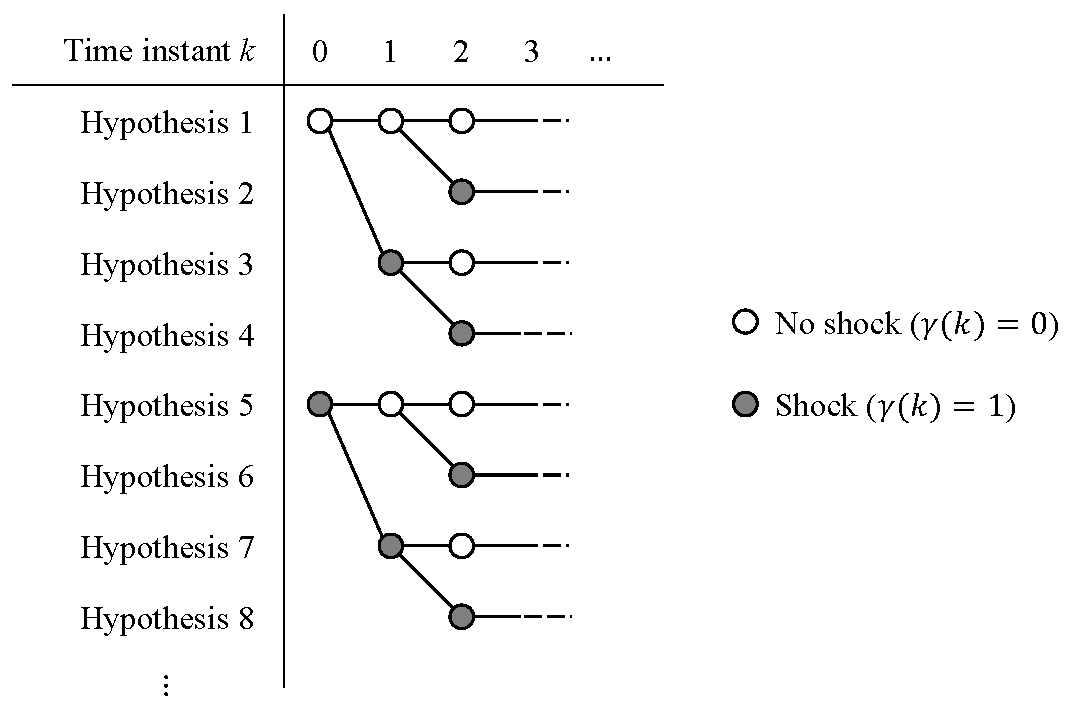
\includegraphics[height=7.5cm]{images/mm_obs_seq_br.pdf}
	\caption{Sequence branching}
	\label{fig:mm-obs-br}
\end{figure}

\subsubsection{Generalised pseudo-Bayes algorithm} \label{sec:GPB}

One of the simplest sub-optimal multiple-model methods is the \textit{generalised pseudo-Bayesian algorithm} \citep{buxbaum_recursive_1969, jaffer_estimation_1971, tugnait_detection_1982}. Although not used directly in this work, the method is described here because it is a starting point for understanding hypotheses branching and merging, which are techniques used in the sequence fusion algorithm described by \cite{robertson_detection_1995}.

There are two basic versions of the algorithm, the \acrlong{GPB1} (\acrshort{GPB1}), and the \acrlong{GPB2} (\acrshort{GPB2}). Figure \ref{fig:mm-obs-gpb1} shows a simplified diagram of the \gls{GPB1} process in the case of a system with two modes ($n_j=2$). A single estimate of the system states and error covariance at time $k$ is branched into $n_j$ hypotheses representing the possible modes of the system at that time. In this context, \textit{branching} simply means duplicating or cloning the hypothesis state estimates and error covariance into $n_j$ copies. These are then used to initialise $n_j$ Kalman filters. Each Kalman filter then makes a prediction of the states in the next time instant using the system model associated with one of the possible modes. In the next time instant, the $n_j$ predictions are corrected using the measurements, and the updated estimates are merged into a single set of estimates using the multiple-model observer merging procedure defined by (\ref{eq:xkyk_hat_MKF}, \ref{eq:Pk_MKF}). These branching and merging steps are then repeated at each subsequent time step.
\begin{figure}[ht]
	\centering
	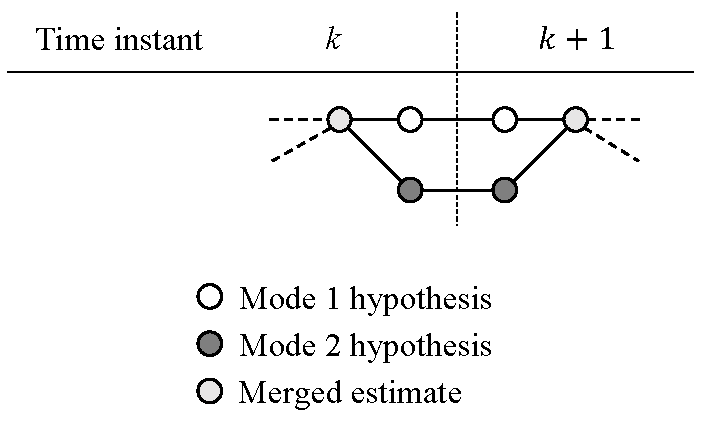
\includegraphics[height=5cm]{images/mm_obs_seq_gpb1.pdf}
	\caption{Simplified diagram of the \gls{GPB1} algorithm ($n_j=2$)}
	\label{fig:mm-obs-gpb1}
\end{figure}

Whereas the \gls{GPB1} estimator considers $n_j$ possible mode transitions from time $k-1$ to time $k$, the \gls{GPB2} estimator considers $n_j^2$ possible transition sequences from time $k-2$ to time $k$. Figure \ref{fig:mm-obs-gpb2} shows a simplified diagram of the \gls{GPB2} algorithm in the case of two system modes ($n_j=2$). At time $k$ it maintains $n_j$ merged estimates and associated variables, $\left\{ \hat{\mathbf{x}}_m(k \mid k), \mathbf{P}_m(k \mid k), \hat{\mathbf{y}}_m(k \mid k), \Pr(\Gamma_m(k) \mid \mathbf{Y}_M(k)) \right\}$, for $m=1,2,...,n_j$. Each of these is then branched into $n_j$ estimates, creating a total of $n_h=n_j^2$ hypotheses, represented by $n_h$ Kalman filters labelled $f=1,2,...n_h$. At time $k+1$, the Kalman filter predictions are corrected to produce $n_h$ estimates. Then, two merging operations are carried out on these estimates. The first merges the $n_h$ estimates into $n_m=n_j$ estimates for use in the next step. The second merges the $n_m$ merged estimates again, into one final estimate which is the output of the observer and is not used in subsequent steps.
\begin{figure}[ht]
	\centering
	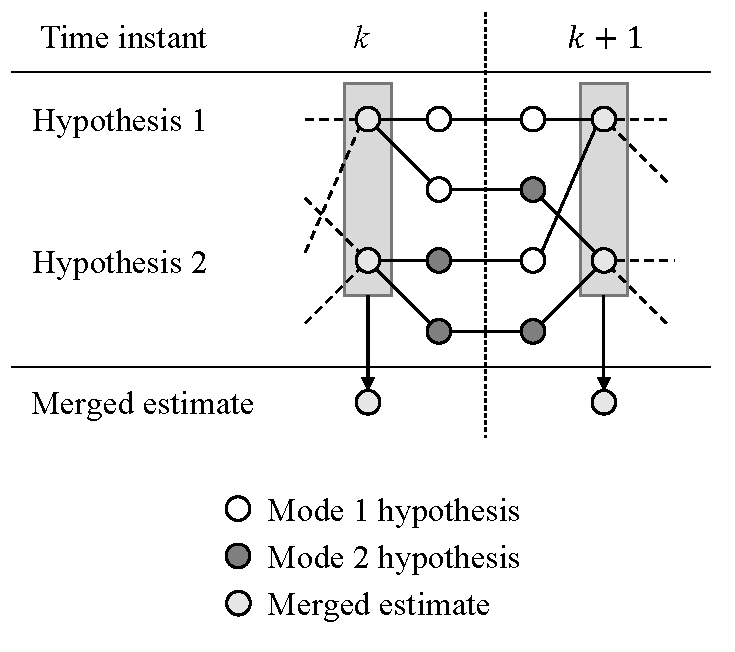
\includegraphics[height=6.5cm]{images/gpb2_diagram.pdf}
	\caption{Simplified diagram of the \gls{GPB2} algorithm ($n_j=2$)}
	\label{fig:mm-obs-gpb2}
\end{figure}

The $n_m$ merged estimates and covariances at time $k$ are produced by calculating weighted sums of the estimates and covariances of the branched hypotheses,
\nomenclature{$n_m$}{number of merged hypotheses maintained by a multiple-model observer}%
\nomenclature{$\mathbf{\hat{x}}_m(k \mid k)$}{merged estimates of the system states at time $k$ for merged hypothesis $m$}%
\nomenclature{$\mathbf{\hat{y}}_m(k \mid k)$}{merged estimates of the system outputs at time $k$ for merged hypothesis $m$}%
\nomenclature{$\mathbf{P}_m(k \mid k)$}{merged state estimation error covariance at time $k$ for merged hypothesis $m$}%
\nomenclature{$\Gamma_m(k)$}{merged shock hypothesis $m$ at time $k$}%
\begin{equation} \label{eq:xmkymk_hat_MKF}
	\begin{aligned}
		\mathbf{\hat{x}}_m(k \mid k) = \frac{1}{Z_m(k)} \sum_{f \in \mathcal{H}_{\text{merge},m}} \mathbf{\hat{x}}_f(k \mid k) \Pr(\Gamma_f(k) \mid \mathbf{Y}_M(k)), \\
		\mathbf{\hat{y}}_m(k \mid k) = \frac{1}{Z_m(k)} \sum_{f \in \mathcal{H}_{\text{merge},m}} \mathbf{\hat{y}}_f(k \mid k) \Pr(\Gamma_f(k) \mid \mathbf{Y}_M(k)),\\
		\mathbf{P}_m(k \mid k) = \frac{1}{Z_m(k)} \sum_{f \in \mathcal{H}_{\text{merge},m}} \Pr(\Gamma_f(k) \mid \mathbf{Y}_M(k)) \left( \mathbf{P}_f(k \mid k) + \delta_\mathbf{\hat{x}}(k) \delta_\mathbf{\hat{x}}^\intercal(k) \right), \\
		\delta_\mathbf{\hat{x}}(k) = \mathbf{\hat{x}}_m(k \mid k) - \mathbf{\hat{x}}_f(k \mid k), \\
		\Pr(\Gamma_m(k) \mid \mathbf{Y}_M(k)) = \sum_{f \in \mathcal{H}_{\text{merge},m}} \Pr(\Gamma_f(k) \mid \mathbf{Y}_M(k)).
	\end{aligned}
\end{equation}
\nomenclature{$\mathcal{H}_{\text{merge}}$}{hypothesis index used in merging operations}%
where $\mathcal{H}_{\text{merge}}$ is a set of $n_m$ indices that determine which hypotheses are merged to produce each merged estimate, and $Z_m(k)$ is a scalar normalization variable given by
\nomenclature{$Z_m(k)$}{normalization variable at time $k$ used in merged probability calculations}%
\begin{equation} \label{eq:Zmk}
	Z_m(k) = \sum_{f \in \mathcal{H}_{\text{merge},m}} \Pr(\Gamma_f(k) \mid \mathbf{Y}_M(k)).
\end{equation}

In the case of \gls{GPB2}, $\mathcal{H}_{\text{merge}}$ is defined
\begin{equation} \label{eq:Hmerge_GPB2}
	\mathcal{H}_{\text{merge}} = \begin{Bmatrix} \mathcal{H}_{\text{merge},1} \\ \mathcal{H}_{\text{merge},2} \end{Bmatrix} = \begin{Bmatrix}
		\begin{bmatrix}	1 \\ 3 \end{bmatrix} \\
		\begin{bmatrix}	2 \\ 4 \end{bmatrix}
	\end{Bmatrix}.
\end{equation}
This means that merged estimate $\mathbf{\hat{x}}_1(k \mid k)$ is calculated by merging the estimates associated with branched hypotheses 1 and 3, and merged estimate $\mathbf{\hat{x}}_2(k \mid k)$ is calculated by merging the estimates of branched hypotheses 2 and 4.

An associated index, $\mathcal{H}_{\text{branch}}$, governs the branching operation, which for \gls{GPB2} is
\nomenclature{$\mathcal{H}_{\text{branch}}$}{hypothesis index used in branching operations}%
\begin{equation} \label{eq:Hbranch_GPB2}
	\mathcal{H}_{\text{branch}} = \begin{bmatrix} 1 \\ 1 \\ 2 \\ 2 \end{bmatrix}.
\end{equation}
This indicates that branched estimates 1 and 2 are clones of merged estimate $\mathbf{\hat{x}}_1(k \mid k)$ and branched estimates 3 and 4 are clones of merged estimate $\mathbf{\hat{x}}_2(k \mid k)$. These definitions match the branching and merging operations depicted in Figure \ref{fig:mm-obs-gpb2}.

% TODO: We don't need this if we define the r(k) and r_m(k) transitions.
The system modes, which determine the system model parameters as well as the mode transition probabilities, evolve according to the branching and merging indices. Starting with the modes associated with the merged hypotheses at time $k$, which in the case of GPB2 are
\nomenclature{$\mathbf{r}_m(k)$}{indicators of the system modes of the merged hypotheses at time $k$ used in branching and merging operations}%
\begin{equation} \label{eq:rmk_GPB2}
		\mathbf{r}_m(k) = \begin{bmatrix} 1 \\ 2 \end{bmatrix},
\end{equation}
the branched modes after branching at time $k$ and before merging at time $k+1$ are
\nomenclature{$\mathbf{r}_{b,1}(k)$}{indicators of the system modes of the branched hypotheses at time $k$ before merging}%
\nomenclature{$\mathbf{r}_{b,2}(k)$}{indicators of the system modes of the branched hypotheses at time $k$ after branching}%
\begin{equation} \label{eq:rbk_GPB2}
	\begin{aligned}
		\mathbf{r}_{b,2}(k) &= \begin{bmatrix} 1 \\ 1 \\ 2 \\ 2 \end{bmatrix},
		\mathbf{r}_{b,1}(k+1) &= \begin{bmatrix} 1 \\ 2 \\ 1 \\ 2 \end{bmatrix}.
	\end{aligned}
\end{equation}
Note that $\mathbf{r}_{b,2}(k)$ is derived by branching $\mathbf{r}_m(k)$ using $\mathcal{H}_{\text{branch}}$ and that when $\mathbf{r}_{b,1}(k+1)$ is merged using $\mathcal{H}_{\text{merge}}$ in the next time step, it leads to 
\begin{equation} \label{eq:rmkp1rmk_GPB2}
	\mathbf{r}_m(k+1) = \begin{bmatrix} 1 \\ 2 \end{bmatrix} = \mathbf{r}_m(k).
\end{equation}
Due to this condition, the algorithm is consistent when executed consecutively every time step.

The advantages of the \gls{GPB1} and \gls{GPB2} estimators are their simplicity, the fact that they can be applied to any switching system, and that the number of hypotheses ($n_j$ or $n_j^2$) is finite and constant, which limits computational requirements. The disadvantages include the fact that they model every possible transition over one or two time steps and merge these into a reduced set of estimates before the next iteration. 

While the branching, modes, and merging steps of the \gls{GPB1} and \gls{GPB2} algorithms are the same each time step, they may be time-varying in the case of the sub-optimal multiple-model algorithms considered in this work. The notation above is easily extended to more complex algorithms with arbitrary branching and merging steps by allowing $\mathcal{H}_{\text{branch}}$, $\mathcal{H}_{\text{merge}}$, $\mathbf{r}_{b,1}(k)$, and $\mathbf{r}_{b,2}(k)$ to be time-varying and by allowing an arbitrarily large number of branched and merged hypotheses, $n_h$ and $n_m$, to exist at each time instant.

\subsubsection{Sequence fusion} \label{sec:fusion}

\cite{robertson_detection_1995} proposed a sub-optimal approach that combines three approximation techniques specifically intended for \gls{RODD} state estimation. The first is referred to as \textit{sequence fusion}. This is based on the assumption that only recent differences in the hypothesis sequences are important for state estimation. Therefore, sequences that are identical over the previous $N_f$ sample times may be merged, where $N_f$ is known as the \textit{fusion horizon}.
\nomenclature{$N_f$}{sequence fusion parameter: length of fusion horizon in number of sampling intervals}%
%The same techniques used in the generalized pseudo-Bayes algorithm are used to perform the sequence branching and merging at each time step. The differences are that more than $n_j^2$ hypotheses are maintained and these are based on longer, pre-specified sequences of possible shocks.

Rather than allowing the number and length of the shock indicator hypothesis sequences, $\Gamma_f(k)$, to grow indefinitely, a fixed number of sequences of length $N_f$ sample periods are defined, each consisting of only the current and the previous $N_f-1$ values of \hl{$\gamma(k)$}
\nomenclature{$\Gamma_m(k-N_f+1,k)$}{merged shock hypotheses $m$ at time $k$ for the fusion horizon $N_f$}%
\begin{equation} \label{eq:Gamma_kmf_k}
	\Gamma_m(k-N_f+1,k) = \{\gamma_m(k-N_f+1), ...,  \gamma_m(k-1), \gamma_m(k)\}, m=1,2,..., n_m.
\end{equation}
These fixed-length sequences are used to merge similar hypotheses so that the total number, $n_m$, remains the same from one time instant to the next.

Secondly, they assume that the exact timing of random shocks is not important and define \textit{detection intervals} of more than one sample period during which it is assumed that only one shock may occur. This is based on the observation that when the correction gain of a Kalman filter increases due to the assumption of a shock occurrence ($\gamma_m(k)=1$), it tends to remain large for several sample periods. The probability of at least one random shock during a detection interval of length $d$ samples is therefore higher than the probability, $\varepsilon$, of a single shock in one sample period, and is given by
\nomenclature{$d$}{sequence fusion parameter: shock spacing or length of detection interval, in number of sampling intervals}
\nomenclature{$\varepsilon_d$}{sequence fusion parameter: probability of at least one shock within the detection interval}%
\begin{equation}  \label{eq:p_gamma_d}
	\varepsilon_d = 1 - (1 - \varepsilon)^{d}.
\end{equation}

The occurrence of one or more shocks within a detection interval is then represented by a single shock at the start of the detection interval and the probabilities of a shock at any other time are set to zero,
\begin{equation} \label{eq:Pr_gamma_nd}
	\begin{aligned}
		\Pr\left(\gamma_{f}(k)=0\right) = \begin{cases*}
			1 - \varepsilon_d & \text { for } $k = d, 2d, 3d, \ldots$ \\
			1 & \text { for } $k \ne d, 2d, 3d, \ldots$
		\end{cases*} \\
		\Pr\left(\gamma_{f}(k)=1\right) = \begin{cases*}
			\varepsilon_d & \text { for } $k = d, 2d, 3d, \ldots$ \\
			0 & \text { for } $k \ne d, 2d, 3d, \ldots$
		\end{cases*} \\
	\end{aligned}
\end{equation}

Thirdly, they rely on the fact that the random shocks occur infrequently and therefore the probability of more than $n_\text{max}$ shocks during the fusion horizon is low, where $n_\text{max}$ may be 1 or some other low number. This further reduces the number of possible hypotheses that must be modelled.
\nomenclature{$n_\text{max}$}{sequence fusion parameter: maximum number of shock occurrences within the fusion horizon}%

To illustrate the resulting shock hypothesis sequences, consider an example. Suppose there is one \gls{RODD} to estimate. A sequence fusion algorithm is used with a fusion horizon of $N_f=9$, a detection interval of $d=3$, and a maximum number of shocks over the fusion horizon of $n_\text{max}=1$. Figure \ref{fig:mm-obs-seq-SFex1} shows the four shock hypotheses that would be required in this case. Note that hypothesis 1 assumes no shocks at any time. Hypothesis 2 assumes shocks occur at times $k=0,9,18,...$. Hypothesis 3 assumes shocks occur at times $k=3,12,21,...$, and so on. After $N_f=9$ sample periods, the sequences repeat indefinitely.

\begin{figure}[ht]
	\centering
	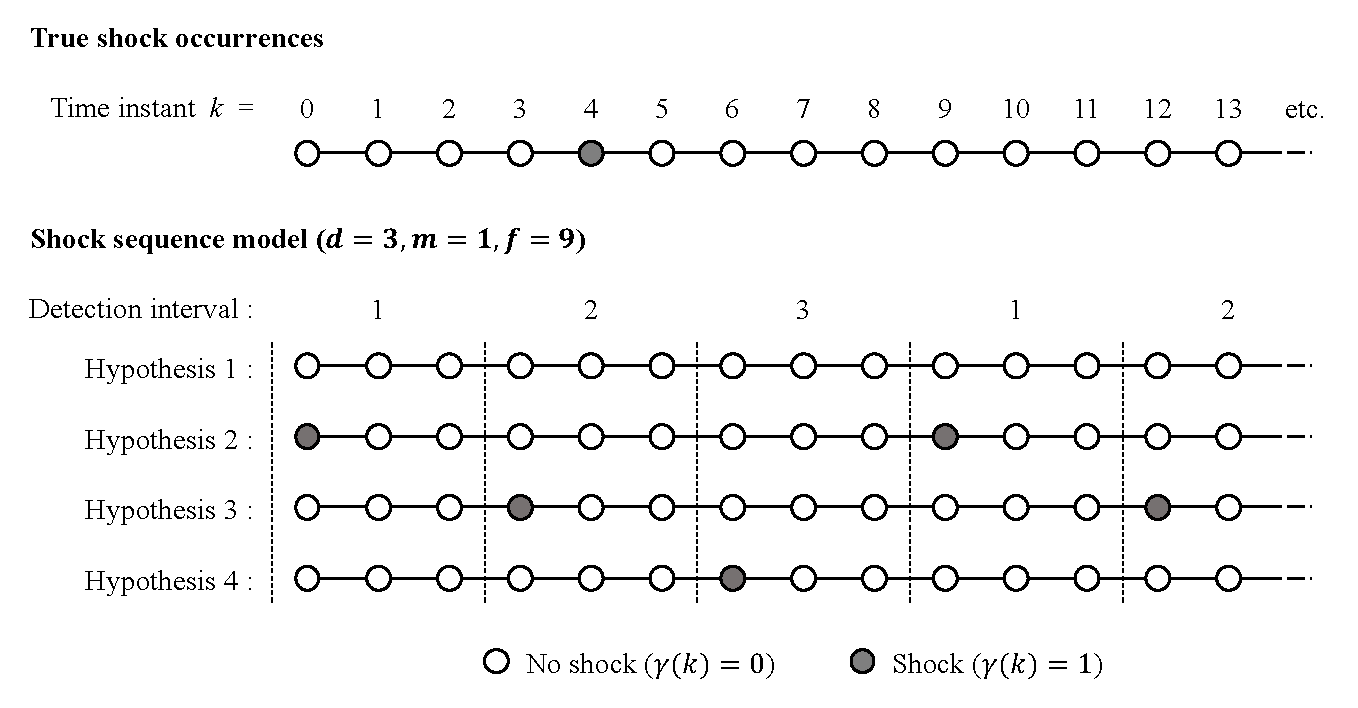
\includegraphics[width=13.5cm]{images/mm_obs_seq_rob1.pdf}
	\caption{Sequence fusion example 1 ($N_f=9$, $n_\text{max}=1$, $d=3$)}
	\label{fig:mm-obs-seq-SFex1}
\end{figure}

Suppose that a shock actually occurred in the system at time $k=4$. In this case, the algorithm should predict that hypothesis 3 is the most likely because this assumes a shock occurred at $k=3$, which is the closest to the actual time.

Figure \ref{fig:mm-obs-seq-SFex2} illustrates a second example with $N_f=10$, $n_\text{max}=2$, and $d=5$. This also has four hypotheses. However, note that hypothesis 4 accounts for the possibility of two shocks within the fusion horizon. As in the previous example, if a true shock occurred at time $k=4$, the most likely hypothesis should be hypothesis 3 because it assumes a shock occurred at $k=5$, which is close to the actual time.
\begin{figure}[ht]
	\centering
	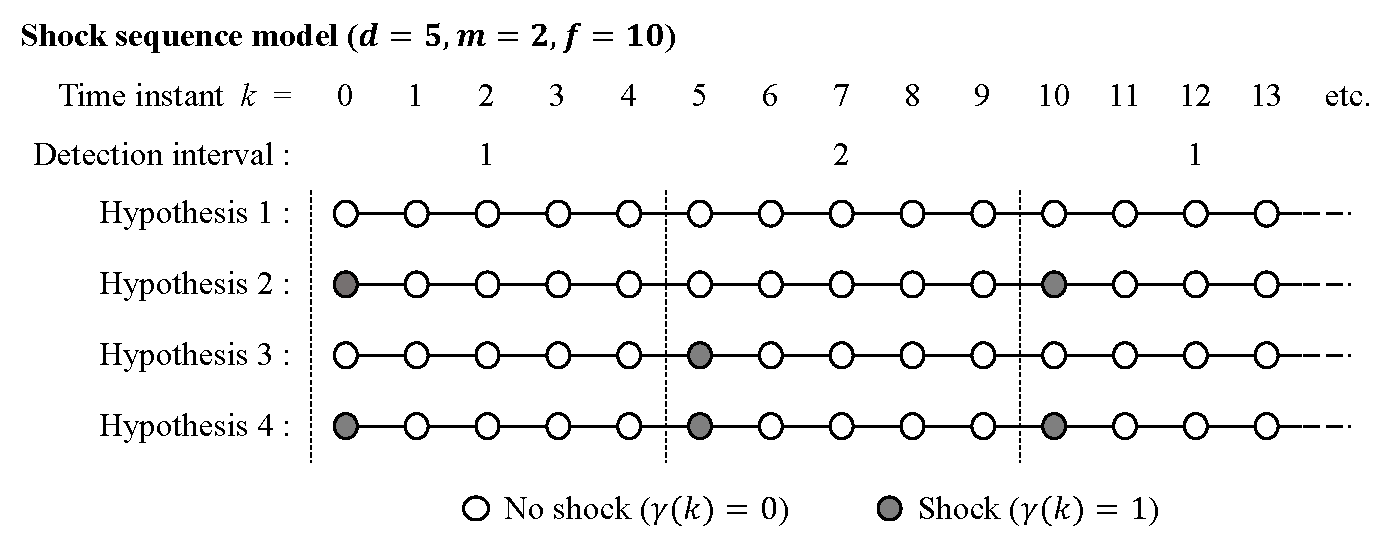
\includegraphics[width=13.5cm]{images/mm_obs_seq_rob2.pdf}
	\caption{Sequence fusion example 2 ($N_f=10$, $n_\text{max}=2$, $d=5$)}
	\label{fig:mm-obs-seq-SFex2}
\end{figure}

As mentioned, the shock hypothesis sequences over the fusion horizon, $\Gamma_m(k-N_f+1,k)$, determine the branching and merging operations that occur at each time step. The logic is as follows: (i) at time $k$, branch each hypothesis sequence into the possible mode transitions that occur between time $k$ and $k+1$, (ii) advance the branched sequences into the next time step, according to the possible mode transitions, (iii) compare the branched sequences and merge those that are identical over the new fusion horizon from time $k-N_f+2$ to $k+1$.

Consider again the sequences from the previous example in Figure \ref{fig:mm-obs-seq-SFex2}. By applying the logic described above, the branching and merging operations depicted in Figure \ref{fig:mm-obs-seq-sf95} may be deduced. For example, consider what happens at time $k=9$. At this time, the fusion horizon spans from time 0 to 9. The four sequences are branched into eight and advanced to the next time instant according to the possible modes at that time (no shock, shock). Then, at time $k=10$ the 8 branched hypotheses are merged back to 4 by combining sequences that are identical over the new fusion horizon, which spans from $k=1$ to 10. Applying this logic each time step, branching and merging are only required once every 5 time steps when shocks are assumed to be possible.
\begin{figure}[ht]
	\centering
	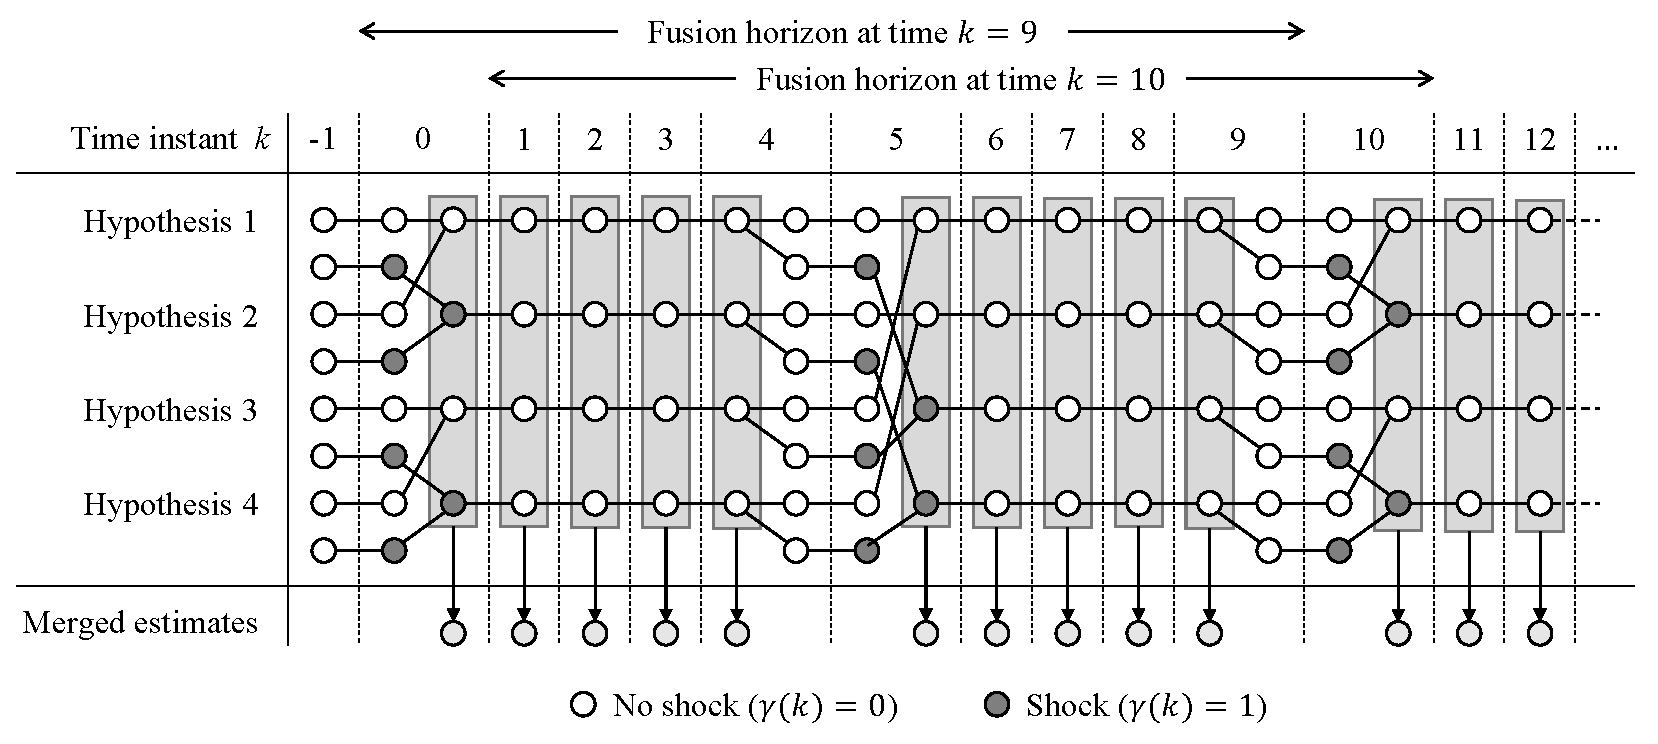
\includegraphics[width=15.5cm]{images/mm_obs_seq_sf95.pdf}
	\caption{Sequence branching and merging example ($N_f=10$, $n_\text{max}=2$, $d=5$)}
	\label{fig:mm-obs-seq-sf95}
\end{figure}

Rather than constant branching and merging indices, as in GPB2 (\ref{eq:Hbranch_GPB2}, \ref{eq:Hmerge_GPB2}), sequences of branching and merging indices are needed. In this example, they are
\begin{equation} \label{eq:Hbranch_SFex2}
	\mathcal{H}_{\text{branch}} = \begin{Bmatrix}
		\begin{bmatrix} 1 \\ 2 \\ 3 \\ 4 \end{bmatrix} &
		\begin{bmatrix} 1 \\ 2 \\ 3 \\ 4 \end{bmatrix} &
		\begin{bmatrix} 1 \\ 2 \\ 3 \\ 4 \end{bmatrix} &
		\begin{bmatrix} 1 \\ 2 \\ 3 \\ 4 \end{bmatrix} &
		\begin{bmatrix} 1 \\ 1 \\ 2 \\ 2 \\ 3 \\ 3 \\ 4 \\ 4 \end{bmatrix} &
		\begin{bmatrix} 1 \\ 2 \\ 3 \\ 4 \end{bmatrix} &
		\begin{bmatrix} 1 \\ 2 \\ 3 \\ 4 \end{bmatrix} &
		\begin{bmatrix} 1 \\ 2 \\ 3 \\ 4 \end{bmatrix} &
		\begin{bmatrix} 1 \\ 2 \\ 3 \\ 4 \end{bmatrix} &
		\begin{bmatrix} 1 \\ 1 \\ 2 \\ 2 \\ 3 \\ 3 \\ 4 \\ 4 \end{bmatrix}
	\end{Bmatrix},
\end{equation}
and
\begin{equation} \label{eq:Hmerge_SFex2}
	\mathcal{H}_{\text{merge}} = \begin{Bmatrix}
		\begin{bmatrix}	1 \\ 3 \end{bmatrix} & 1 & 1 & 1 & 1 & \begin{bmatrix}	1 \\ 5 \end{bmatrix} & 1 & 1 & 1 & 1 \\
		\begin{bmatrix}	2 \\ 4 \end{bmatrix} & 2 & 2 & 2 & 2 & \begin{bmatrix}	3 \\ 7 \end{bmatrix} & 2 & 2 & 2 & 2 \\
		\begin{bmatrix}	5 \\ 7 \end{bmatrix} & 3 & 3 & 3 & 3 & \begin{bmatrix}	2 \\ 6 \end{bmatrix} & 3 & 3 & 3 & 3 \\
		\begin{bmatrix}	6 \\ 8 \end{bmatrix} & 4 & 4 & 4 & 4 & \begin{bmatrix}	4 \\ 8 \end{bmatrix} & 4 & 4 & 4 & 4 \\
	\end{Bmatrix}.
\end{equation}

% Remove these: they don't add anything since these can be derived from the sequence
% and the branching/merging indices. Also, this convention for \Gamma_b and \Gamma_m
% was not defined. \Gamma_f was defined as single sequence and arguably would be
% better restricted to the merged sequences, than the branched ones.
%Likewise, the merged and branched shock (mode) indicator sequences are
%\begin{multline} \label{eq:Gamma_km09}
%	\glsadd{Gammafkmnk}\Gamma_m(0,9) = \left\{
%		\mathbf{\gamma}_m(0), \mathbf{\gamma}_m(1), \cdots, \mathbf{\gamma}_m(9)
%	\right\} = \\ 
%	\left\{
%		\begin{bmatrix} 0 \\ 1 \\ 0 \\ 1 \end{bmatrix},
%		\begin{bmatrix} 0 \\ 0 \\ 0 \\ 0 \end{bmatrix},
%		\begin{bmatrix} 0 \\ 0 \\ 0 \\ 0 \end{bmatrix},
%		\begin{bmatrix} 0 \\ 0 \\ 0 \\ 0 \end{bmatrix},
%		\begin{bmatrix} 0 \\ 0 \\ 0 \\ 0 \end{bmatrix},
%		\begin{bmatrix} 0 \\ 0 \\ 1 \\ 1 \end{bmatrix},
%		\begin{bmatrix} 0 \\ 0 \\ 0 \\ 0 \end{bmatrix},
%		\begin{bmatrix} 0 \\ 0 \\ 0 \\ 0 \end{bmatrix},
%		\begin{bmatrix} 0 \\ 0 \\ 0 \\ 0 \end{bmatrix},
%		\begin{bmatrix} 0 \\ 0 \\ 0 \\ 0 \end{bmatrix}
%	\right\}.
%\end{multline}
%\begin{multline} \label{eq:Gamma_kb09}
%		\Gamma_b(0,9 \mid 9) = \left\{\mathbf{\gamma}_b(0 \mid 0), \mathbf{\gamma}_b(1 \mid 1), \cdots, \mathbf{\gamma}_b(9 \mid 9) \right\} = \\
%		\left\{
%			\begin{bmatrix} 0 \\ 0 \\ 0 \\ 0 \end{bmatrix},
%			\begin{bmatrix} 0 \\ 0 \\ 0 \\ 0 \end{bmatrix},
%			\begin{bmatrix} 0 \\ 0 \\ 0 \\ 0 \end{bmatrix},
%			\begin{bmatrix} 0 \\ 0 \\ 0 \\ 0 \end{bmatrix},
%			\begin{bmatrix} 0 \\ 0 \\ 0 \\ 0 \\ 1 \\ 1 \\ 1 \\ 1 \end{bmatrix},
%			\begin{bmatrix} 0 \\ 0 \\ 0 \\ 0 \end{bmatrix},
%			\begin{bmatrix} 0 \\ 0 \\ 0 \\ 0 \end{bmatrix},
%			\begin{bmatrix} 0 \\ 0 \\ 0 \\ 0 \end{bmatrix},
%			\begin{bmatrix} 0 \\ 0 \\ 0 \\ 0 \end{bmatrix}
%			\begin{bmatrix} 0 \\ 0 \\ 1 \\ 1 \\ 0 \\ 0 \\ 1 \\ 1 \end{bmatrix},
%		\right\},
%\end{multline}
%\begin{multline} \label{eq:Gamma_kb110}
%		\Gamma_b(1,10 \mid 9) = \left\{ \mathbf{\gamma}_b(1 \mid 0), \mathbf{\gamma}_b(2 \mid 1), \cdots, \mathbf{\gamma}_b(10 \mid 9) \right\} = \\
%		\left\{
%			\begin{bmatrix} 0 \\ 1 \\ 0 \\ 1 \\ 0 \\ 1 \\ 0 \\ 1 \end{bmatrix},
%			\begin{bmatrix} 0 \\ 0 \\ 0 \\ 0 \end{bmatrix},
%			\begin{bmatrix} 0 \\ 0 \\ 0 \\ 0 \end{bmatrix},
%			\begin{bmatrix} 0 \\ 0 \\ 0 \\ 0 \end{bmatrix},
%			\begin{bmatrix} 0 \\ 0 \\ 0 \\ 0 \end{bmatrix},
%			\begin{bmatrix} 0 \\ 1 \\ 0 \\ 1 \\ 0 \\ 1 \\ 0 \\ 1 \end{bmatrix},
%			\begin{bmatrix} 0 \\ 0 \\ 0 \\ 0 \end{bmatrix},
%			\begin{bmatrix} 0 \\ 0 \\ 0 \\ 0 \end{bmatrix},
%			\begin{bmatrix} 0 \\ 0 \\ 0 \\ 0 \end{bmatrix},
%			\begin{bmatrix} 0 \\ 0 \\ 0 \\ 0 \end{bmatrix}
%		\right\}.
%\end{multline}
Although the number of branched hypotheses is time-varying, after $N_f$ time steps the sequences repeat such that
\nomenclature{$\mathbf{\gamma}_m(k)$}{vector of random shock indicators, $\gamma_f(k)$ for $f=1,2,...,m$, at time $k$}%
\begin{equation} \label{eq:rmkrmkmNf_SFex2}
	\mathbf{\gamma}_m(k) = \mathbf{\gamma}_m(k-N_f).
\end{equation}

As in the \gls{GPB2} algorithm, the overall estimates of the system states and outputs, $\hat{\mathbf{x}}(k \mid k)$ and $\hat{\mathbf{y}}(k \mid k)$, are calculated by merging the partially-merged estimates into one overall estimate. This is achieved by substituting $\mathbf{\hat{x}}_m(k \mid k)$ and $\mathbf{\hat{y}}_m(k \mid k)$ for $\mathbf{\hat{x}}_f(k \mid k)$ and $\mathbf{\hat{y}}_f(k \mid k)$ in \eqref{eq:xkyk_hat_MKF}.

\cite{robertson_detection_1995} described a systematic procedure to choose the parameters $N_f$, $n_\text{max}$, and $d$ and give the formula for the total probability of the modelled hypotheses as
\begin{equation} \label{eq:p_gamma}
	\beta=\operatorname{Pr}\left(\sum_{i=1}^{n} \gamma(i d) \leq n_\text{max} \right) = \sum_{j=0}^{n_\text{max}} \binom{n}{j} \varepsilon_d^{n-j}(1-\varepsilon_d)^{j},
\end{equation}
\nomenclature{$\beta$}{sequence fusion paramter: total probability of the modelled hypotheses, or in the case of the \acrshort{BRW}, a parameter of the additive bias function $a(\cdot)$}%
where $\binom{n}{j}$ represents the number of possible combinations of $j$ shocks in $n$ detection intervals. They recommended that the total probability should be at least 0.99 to ensure that only low-probability hypotheses are ignored.

In a later journal paper, \cite{robertson_method_1998} described a variation to the sequence fusion algorithm described above.  Rather than assuming that the shock occurs in the first sample period of each detection interval, as shown in Figures \ref{fig:mm-obs-seq-SFex1} and \ref{fig:mm-obs-seq-SFex2}, they proposed to represent the possibility of a shock as a sequence of $d$ smaller shocks such that the total variance over the detection interval is the same as that of one shock. They claimed this improved the performance of the algorithm in their simulations.

To implement this modification, define a new variable, $\delta(n)$, to represent whether or not at least one shock occurred during the $n$\textsuperscript{th} detection interval:
\nomenclature{$\delta(n)$}{sequence fusion variable: indicator of whether one or more shocks occurred in detection interval $n$}
\begin{equation} \label{eq:deltak}
	\delta(n) = \begin{cases*}
		0 & \text{if} $\sum_{k=(n-1) d}^{n d - 1}{\gamma(k)} = 0$, \\
		1 & \text{if} $\sum_{k=(n-1) d}^{n d - 1}{\gamma(k)} \ge 1$.
	\end{cases*}
\end{equation}

Then, replace the random shock variable used at each sample time, $w_p(k)$ \eqref{eq:wpk2}, with:
\begin{equation} \label{eq:wpdk}
	w_{p,d}(k) \sim 
	\begin{cases*}
		\mathcal{N}\left(0, \sigma_{w_p}^2\right) & \text{when} $\delta(n) = 0$, \\
		\mathcal{N}\left(0, \frac{b^2\sigma_{w_p}^2}{d}\right) & \text{when} $\delta(n) = 1$.
	\end{cases*}
\end{equation}

Note that the variance of a single shock, $b^2\sigma_{w_p}^2$, has ben divided by the detection interval length $d$. In this version of the algorithm, the branching and merging operations are only carried out at the end of each detection interval. In the steps within the detection interval, the Kalman filters are updated using the measurements, but no branching or merging occurs.

Figure \ref{fig:mm-obs-seq-sf98} shows the shock hypothesis sequences and the merging and branching steps of the 1998 version of the sequence fusion algorithm with the same parameters as in the previous example.
\begin{figure}[ht]
	\centering
	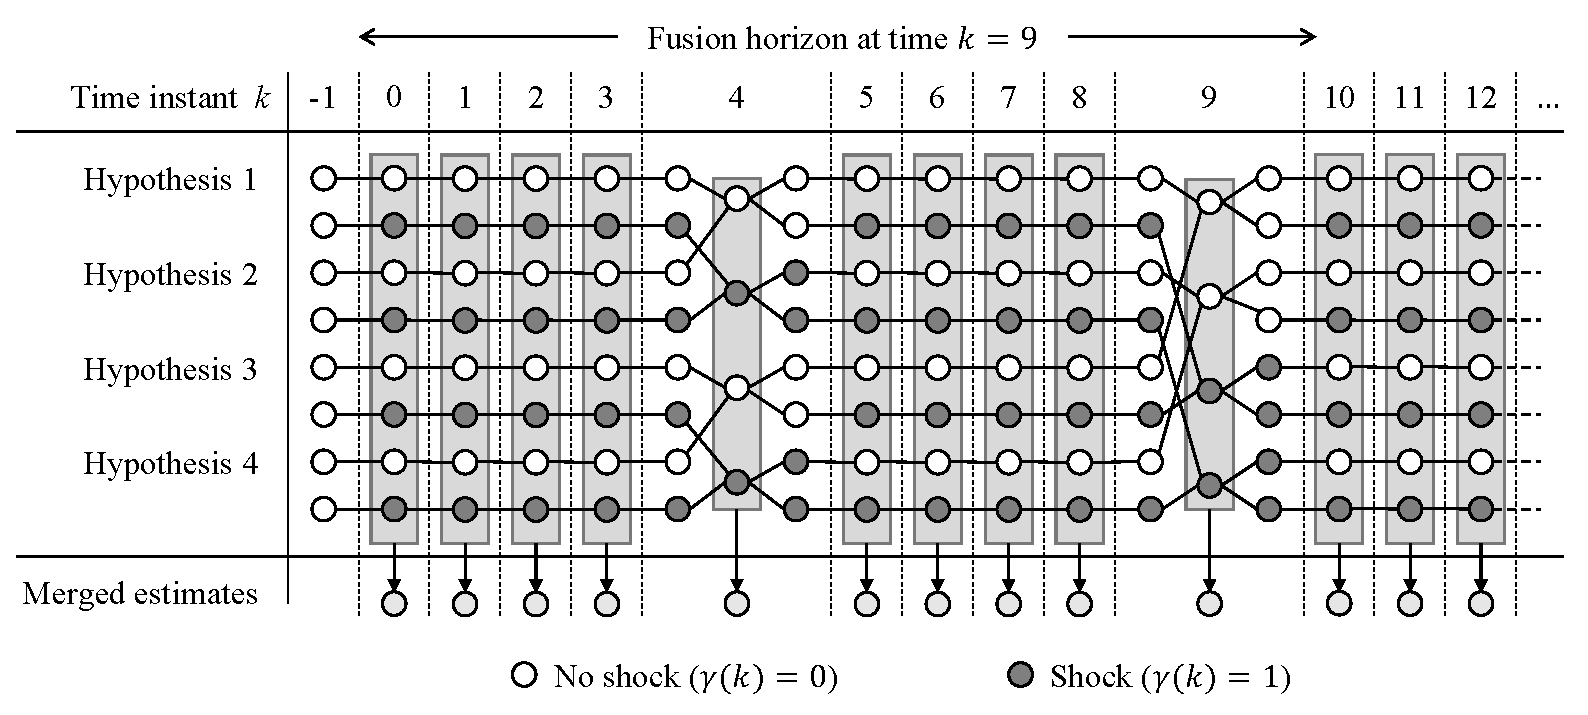
\includegraphics[width=15cm]{images/mm_obs_seq_sf98.pdf}
	\caption{Sequence branching and merging example – 1998 version ($N_d=5$, $n_\text{max}=2$, $N_f=10$)}
	\label{fig:mm-obs-seq-sf98}
\end{figure}
Note the two main differences when compared to Figure \ref{fig:mm-obs-seq-sf95}. Firstly, the system mode indicators are the same throughout the detection interval, whereas in the 1995 version the shocks were assumed to occur only at the first sample time of each detection interval. Secondly, after branching, the $n_h$ hypotheses are maintained for the duration of the detection interval before being merged and branched at the last sample time of the detection interval. The idea of these modifications is to allow $N_d$ Kalman filter updates to occur with the adjusted shock probability and variance (\ref{eq:p_gamma_d}, \ref{eq:wpdk}) before evaluating and merging the estimates. This was expected to produce better estimates of the hypothesis probabilities in situations where it takes more than one time step to detect changes in the system.

\subsubsection{Sequence pruning} \label{sec:pruning}

\textit{Sequence pruning} is the selective deletion of shock hypotheses that have a low likelihood given the current measurements. \cite{eriksson_classification_1996} used the \textit{adaptive forgetting through multiple models} (\acrshort{AFMM}) algorithm by \cite{andersson_adaptive_1985} for \gls{RODD} estimation. The \gls{AFMM} uses sequence pruning to limit the number of hypotheses and filters. The current hypotheses at each time instant are ranked according to their conditional probabilities \eqref{eq:Pr_Gammak_given_Yk}. The hypothesis with the lowest probability is then pruned with the caveat explained below. The most probable hypothesis is allowed to branch but all other hypotheses are advanced assuming no shock occurs in the next time period (i.e. all but one of their branches are pruned). This makes sense in the case of \gls{RODD} disturbances because the probability of a shock is low. Thus, the total number of hypotheses and filters is capped at a fixed number, $n_h$.

The caveat mentioned above, is that no hypothesis may be eliminated less than $N_\text{min}$ time steps after being created. This is to prevent good hypotheses from being eliminated before the conditional probabilities have been properly estimated, which can take more than one sample period. For this reason, $n_h$ must be at least sufficient to accommodate the \textit{minimum life}, $N_\text{min}$, of all new hypotheses. Note that in the case of systems with more than one \gls{RODD} disturbance, the number of branches of the most likely sequence is more than two, \hl{and the same number} of sequences will be pruned at each sample time.
\nomenclature{$N_\text{min}$}{sequence pruning parameter: minimum life of a branched hypothesis in number of sampling intervals}%

To illustrate the sequence pruning procedure, consider the diagram in Figure \ref{fig:mm-obs-seq-SP}. This shows one possible evolution of the hypothesis sequences in response to an actual shock sequence consisting of one shock at time $k=4$.  The most likely hypotheses at each time instant, identified by the circles with thicker outlines, branch into two at the next time instant. After the limit of five hypotheses is reached, one hypothesis is pruned at each sample time and replaced by a new branched hypothesis at the next. Note that at time $k=6$, hypothesis 2 becomes the most likely based on the available measurements at that time. Also note that no new branches are terminated in less than two sample times.
\begin{figure}[ht]
	\centering
	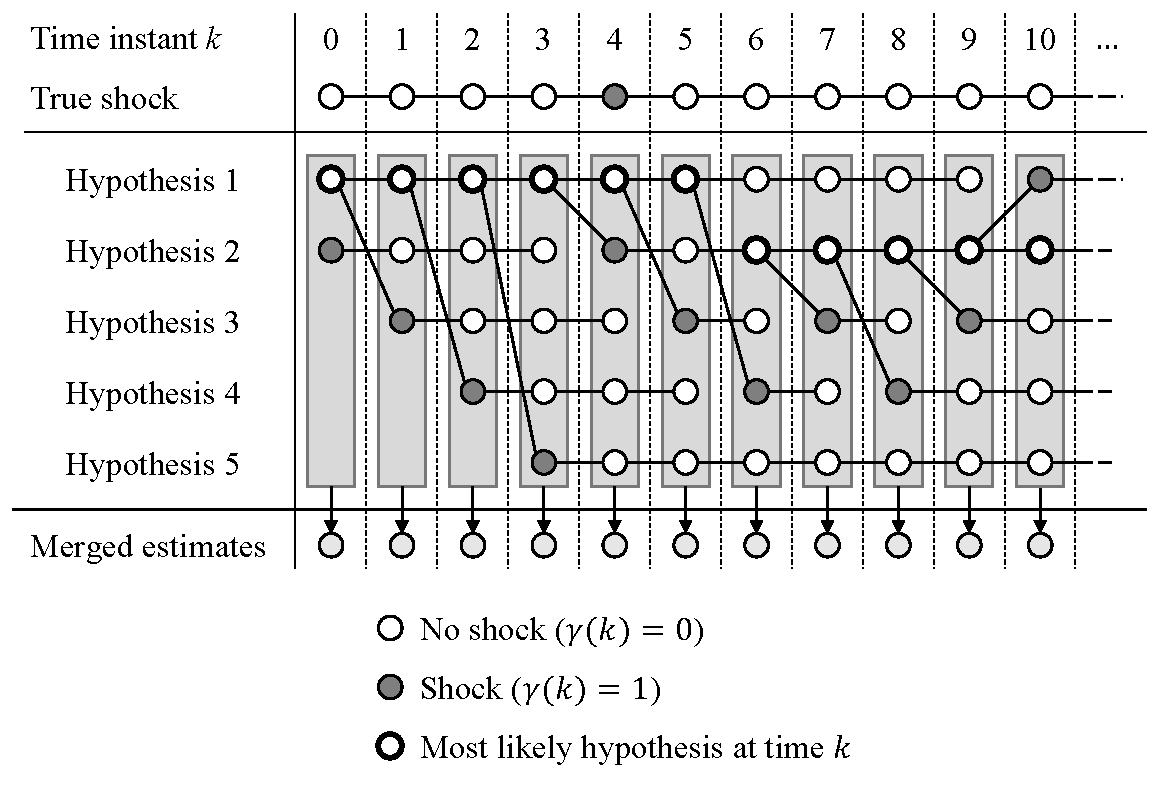
\includegraphics[width=10.7cm]{images/mm_obs_seq_SP.pdf}
	\caption{Sequence pruning example ($n_h=5$, $N_\text{min}=2$)}
	\label{fig:mm-obs-seq-SP}
\end{figure}

The \gls{AFMM} algorithm includes a complementary procedure for online estimation of the measurement noise covariance, $\mathrm{R}(k)$. This component was not implemented in this work since it is assumed that the variance of the measurement noise is time-invariant.

\subsubsection{Implementation details} \label{sec:implementation}

The diagram in Figure \ref{fig:mkf-infoflow} depicts the general computation steps and information flows of the sub-optimal multiple-model observers, as implemented in this work. The solid black rectangles represent computation steps and the \hl{coloured lines} represent the main variables. Steps 1 and 2 are the prediction steps of the Kalman filters (\ref{eq:xfkp1_hat}, \ref{eq:yfk_pred}), step 3 is the calculation of the prior probabilities of the hypotheses \eqref{eq:Pr_Gammak_given_Ykm1}, step 4 is the hypotheses evaluation step (\ref{eq:Pr_Gammak_given_Yk}, \ref{eq:qfk}), and step 5 is the Kalman filter update step (\ref{eq:xfkyfk_hat}, \ref{eq:Pkf-stab}). Step 6 is a place-holder for the sub-optimal procedures which depend on the specific algorithm but in this work include some combination of sequence branching, pruning, and merging. During this step, the final estimates of the states and outputs are also calculated.

\begin{figure}[ht]
	\centering
	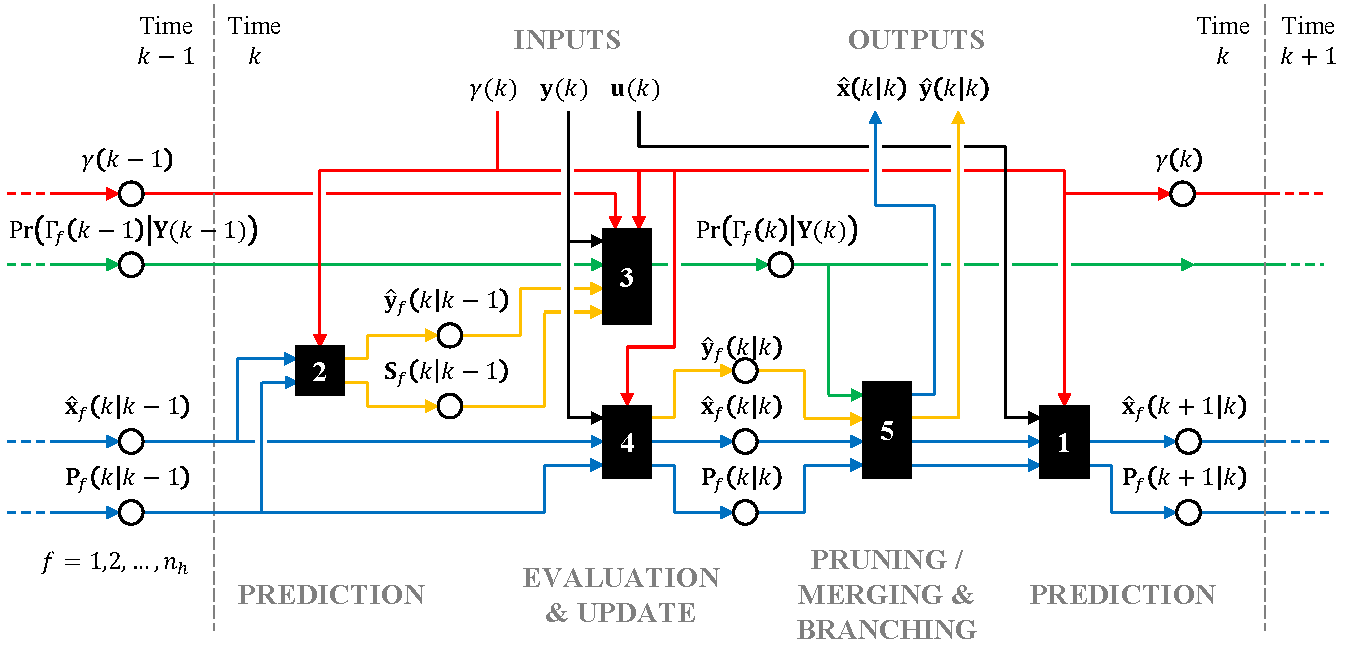
\includegraphics[width=15.5cm]{images/mkf_infoflow.pdf}
	\caption{General information flow diagram of a multiple-model observer}
	\label{fig:mkf-infoflow}
\end{figure}

At time $k$, the algorithm requires a mode indicator vector, $\gamma(k)=\begin{bsmallmatrix} \gamma_1(k) & \cdots & \gamma_{n_h}(k) \end{bsmallmatrix}^\intercal$, the system output measurement, $\mathbf{y}_M(k)$, and input, $\mathbf{u}(k)$, and produces estimates of the states, $\hat{\mathbf{x}}(k \mid k)$, and outputs, $\hat{\mathbf{y}}(k \mid k)$. The mode indicator vector is either constant, as in the case of the \gls{GPB1} and \gls{GPB2} algorithms or is specified by the sub-optimal procedure at each time step. At the end of each time step, the mode indicator vector, conditional hypothesis probabilities, one-step-ahead state predictions, and the prediction error covariances for each hypothesis are stored for use in the next time step. The sub-optimal algorithm, which determines $\gamma(k)$ as well as the merging, pruning, and branching procedures in step 6, may have other variables that need to be stored. These are not shown on the diagram. The total number of hypotheses modelled, $n_h$, also depends on the algorithm, and may be time-varying.

\section{System identification} \label{sec:sys-id}

% Some text not used in IFAC report
Model-based observers such as the Kalman filter require a dynamic model of the process. In practice, models of the process dynamics are not available but they can be identified when input-output data sampled from the process is available. In this case, system identification methods are common practice, as described by \cite{ljung_system_1999} among others.

To construct a multiple-model observer for systems with \gls{RODD}s, the structure and parameters of the disturbance model as well as the process model are needed. \gls{RODD}s are discrete-time \acrlong{MJLS} (\acrshort{MJLS}) \citep{costa_discrete-time_2005}. Standard approaches to system identification such as least-squares regression are not applicable to hybrid dynamical systems with both discrete and continuous states. Identification of these types of systems is challenging and the subject of ongoing research. See for example, \cite{piga_estimation_2020}.

%Outline notes:
%\begin{itemize}
%	\item Explain Isaksson and Eriksson's perspective on standard system identification approach.
%	\item Explain distinction between system detection or `discrimination' and system identification, reference Isaksson and Eriksson's paper on disturbance classification (whether disturbance at input or output of process).
%	\item Introduce other approaches—MLE, EM algorithm (Dempster et al., Wong \& Lee)
%	\item Methods proposed by Bemporad (Fitting jump models, 2018 and Jump Box-Jenkins, 2020).
%	\item Theory and challenges Costa book. Others?
%	\item In recent years, numerical methods to overcome the intractability of the probabilistic integral have received a lot of attention.
%	\item Sequential Monte-Carlo methods, (incl. particle filtering), Stochastic Variational Inference, ... (read Special issue in IEEE control magazine for an overview of these methods)
%\end{itemize}

% More text from IAFAC paper:
%are assumed to be known and were set to match the characteristics of the simulated disturbance. In practice, they would have to be estimated, either using prior knowledge of the disturbance source, or possibly from system output measurements using an appropriate system identification method---see \cite{schon_sequential_2015} for one possible approach---provided a sufficiently long sequence of data is available.

% Note: may remove this if we aren’t using any formal methods.

%\section{Control strategies}
%
%In this work, the goal is to test the performance of different observers in a closed-loop feedback control application (not to evaluate different control strategies). Therefore, only one control strategy is considered. According to the \textit{separation principle} of estimation and control, the control strategy may be designed independently of the observer. The controller is designed using the same augmented system model, including the plant model and disturbance models, that is used in the observer design. However, the switching behaviour of the random shock variable used in the \gls{RODD} is not explicitly considered in the control design. The estimates of the model states produced by the observer are assumed to be optimal, i.e. the expected values, and their uncertainty is not taken into account by the control algorithm or in its design.
%
%
%\subsection{Model predictive control}
%
%\textit{\acrlong{MPC}} (\acrshort{MPC}) is a well known and widely used multi-variable control algorithm used in industrial applications. This is largely due to the fact that constraints can be imposed on the manipulated variables and control variables, as well as its intuitive design and the ease with which it can be tuned to achieve control objectives \citep{maciejowski_predictive_2002}. Although it is a computationally complex algorithm, numerous proven commercial products exist to enable its implementation.
%
%\gls{MPC} utilizes a prediction equation based on the dynamic model of the system to find feasible future trajectories of the system outputs as a function of the manipulated variables and the states of the model at the current time. The length of the prediction horizon, \gls{Hp}, is defined in terms of the number sample times starting at the next time instant, $k+1$. The predicted outputs over the prediction horizon, calculated at the current time $k$, are denoted $\hat{\textbf{y}}(k+i | k)$ for $i=1,2,...,H_p$. The length of the control horizon, \gls{Hc}, is defined starting at the current time, $k$, and the manipulated inputs are denoted $\mathbf{u}(k+i-1)$ for $i=1,2,...,H_c$. The control horizon is usually shorter than the prediction horizon, in which case, $\mathbf{u}(k+j)=\mathbf{u}(k+H_c-1)$ for $j=H_c,H_c+1,...,H_p$.
%
%The constrained optimization problem, which is solved at each time step, is
%\begin{align} \label{eq:mpc-opt}
%	\begin{split}
%		\min _{\mathbf{u}(k), \mathbf{u}(k+1), \ldots, \mathbf{u} (k+H_c-1)}
%		& \quad \sum_{i=1}^{H_{p}}[\mathbf{\hat{y}}(k+i / k) - \mathbf{r}(k+i)]^\intercal \mathbf{\Phi} [\mathbf{\hat{y}}(k+i / k) - \mathbf{r}(k+i)] \\
%		& \qquad + \sum_{i=1}^{H_{c}}[\Delta \mathbf{u}(k+i-1)]^\intercal \mathbf{\Lambda} [\Delta \mathbf{u}(k+i-1)] \\
%			\end{split} \\
%		\text { subject to: }
%		&\ \mathbf{u}_{min} \leq \mathbf{u}(k+j-1) \leq \mathbf{u}_{max} \quad  j=1,2, \dots, H_{c} \label{eq:mpc-cons-1}, \\
%		& \Delta \mathbf{u}_{min} \leq \Delta \mathbf{u}(k+j-1) \leq \Delta \mathbf{u}_{max} \quad j=1,2, \dots, H_{c}, \label{eq:mpc-cons-2} \\
%		& \mathbf{y}_{min} \leq \mathbf{\hat{y}}(k+j / k) \leq \mathbf{y}_{max} \quad  j=1,2, \dots, H_{p}, \label{eq:mpc-cons-3}
%\end{align}\textbf{[TODO: Consider including slack variables to ensure feasibility]}
%where $\mathbf{r}(k+i)$ for $i=1,2,...,H_p$ is the reference output trajectory, and $\Delta \mathbf{u}(k)$ is the change in the manipulated variable at time $k$, defined as $\Delta \mathbf{u}(k) = \mathbf{u}(k) - \mathbf{u}(k-1)$. The tunable parameters are $H_p$, $H_c$, $\mathbf{\Phi}$, and $\mathbf{\Lambda}$, and the constraints are $\mathbf{u}_{min}$, $\mathbf{u}_{max}$, $\Delta \mathbf{u}_{min}$, $\Delta \mathbf{u}_{max}$, $\mathbf{y}_{min}$, and $\mathbf{y}_{max}$. Note that the last constraint \eqref{eq:mpc-cons-3} only guarantees that the estimate of the system output will not violate the constraints. This does not imply that the true system output will respect them at all times.
%
%Once a solution to the optimization problem is found, only the control actions at the current time, $\mathbf{u}(k)$, are transmitted to the plant. The procedure is then repeated every future time instant to compute the subsequent control actions. This is referred to as \textit{receding horizon control}.


\section{Grinding simulation model} \label{sec:grinding-simulator}

%Outline notes:
%\begin{outline}
%    \1 Assumptions and limitations: constant breakage rate model, relationships between speed, media, trajectories, filling level and breakage not captured.
%	\1 Describe grate, transport delays and cyclone model.
%	\1 Outline any significant changes made from Edgar's model
%	\1 Figure: simulation results showing steady-state characteristics - e.g. power, grind, and throughput vs. fill level and speed.
%	\1 Figure \ref{fig:coarse_fine_psd_plot}: Particle size distributions of feed, recirculating load and product - this should help explain steady-state characteristics.
%	\1 Figure - Step responses of main process variables to changes in ore properties.
%	\1 Selection of particle size distribution as the disturbance variable for this work.
%	\1 Steady-state characteristics with operating points (grind curves)\\
%\end{outline}

A dynamic simulation model of the primary grinding circuit of a gold mine in Quebec is used to simulate the effects of changes in ore feed properties on the grinding circuit over time. The model was developed by \cite{perez_garcia_dynamic_2020} following the methodology described by \cite{grimble_dynamic_2010} and was calibrated to match operating data collected from the plant \citep{perez-garcia_systematic_2020}. Grinding in the \acrshort{SAG} mill is simulated by a \textit{population balance model} with 24 discrete ore particle size intervals and constant specific-energy selection rates (i.e. breakage rates are proportional to total energy consumption) and a constant breakage matrix.

Figure \ref{fig:sag-diag} is a simplified diagram of the simulated \acrshort{SAG} mill, which is in a closed circuit consisting of a feed conveyor, pump box, pump, and a bank of hydro-cyclones.
\begin{figure}[ht]
	\centering
	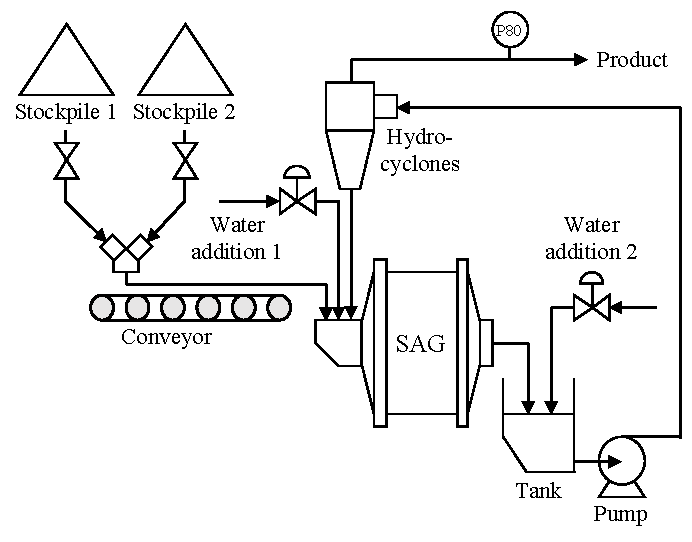
\includegraphics[width=12.5cm]{images/sag-circuit-diag.pdf}
	\caption{Simplified process flow diagram}
	\label{fig:sag-diag}
\end{figure}
For the purposes of this work, two ore feed streams with different \gls{PSD}s were simulated. Each stream is a different mix of two different ores. One ore has a fine \gls{PSD} and the other is coarse. The mix for stream \#1 (`mix 1') consists of 22.83\% coarse ore (\textit{mix factor} of 0.2283) and mix \#2 is an even mix of both ores (mix factor of 0.5). The two streams are mixed before discharging onto the conveyor. Figure \ref{fig:coarse_fine_psd_plot} shows the \gls{PSD}s of the two mixtures.
\begin{figure}[ht]
	\centering
	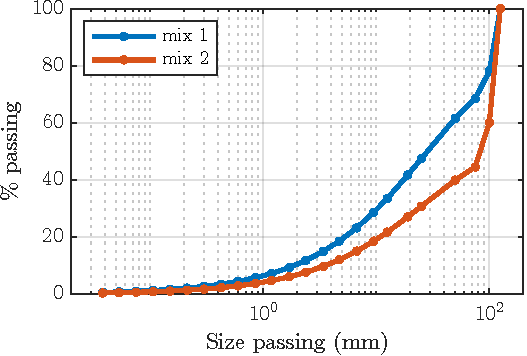
\includegraphics[width=9cm]{images/coarse_fine_cumpsd_plot.pdf}
	\caption{Ore particle size distributions}
	\label{fig:coarse_fine_psd_plot}
\end{figure}

The simulated instrumentation is also illustrated in Figure \ref{fig:sag-diag}. \hl{The setpoint of the water addition flowrate to the mill inlet (`water addition 1') is set to a fixed ratio of the ore feed rate.} The pump-box \hl{(`tank')} has a \gls{PI} controller to control the level to a fixed set-point by manipulating the water addition flow rate set-point (`water addition 2'). The main process variable used in this work is the product P80 measurement, which is a simulated online analyser that estimates the 80\% passing size of the material \hl{in the slurry} leaving the circuit. In this work, the inlet water addition ratio, the conveyor speed, the discharge pump speed, and the mill rotational speed are all fixed.

%The simulated instrumentation is also illustrated in Figure \ref{fig:sag-diag}. The \acrshort{SAG} mill water addition set-point is set by ratio control to a fraction of the fresh ore feed rate, which is measured on the conveyor. This water addition ratio is also manipulated. The pump-box level has a PI (proportional-integral) controller to control the level to a fixed set-point by manipulating the water addition flow rate set-point. The discharge pump speed is fixed. Conveyor speed is adjusted automatically in response to the fresh ore feed rate set-point. The \acrshort{SAG} rotational speed set-point may also be manipulated.
%
%The measurable process variables used in this work are the mill weight, which includes the weight of the shell and liners as well as the mill contents, mill power consumption, the solids-content of the cyclone feed stream, and the particle size (P80) of the ground product in the cyclone overflow. Mill filling level and other simulation variables are available for analysis but are assumed to be unmeasured in the real operation and therefore not available for process control.  Figure \ref{fig:grind_sim_io_diag} summarizes the inputs and outputs of the simulation model. Table \ref{tb:grind-vars} lists the normal operating points, units, and minimum and maximum operating limits of each variable.
%
%%TODO: Table of process variables and normal operating points, limits etc.
%\begin{table}[ht]
%	\centering
%	\caption{Grinding simulation model inputs and outputs} \label{tb:grind-vars}
%	% See: https://texblog.org/2019/06/03/control-the-width-of-table-columns-tabular-in-latex/
%	% Also: https://www.overleaf.com/learn/latex/Tables
%	\begin{tabular}{c c >{\raggedright}p{5.5cm} c c c c}
%		%\toprule
%		& Label & Description & Op. pt. & Units & Min. & Max \\
%		\midrule
%		\multicolumn{7}{l}{\textit{manipulated variables}} \\
%		%\midrule
%		  & MV1       & Ore feed rate & 122.7 & tons/h & 0 & 200 \\   
%		  & MV2       & Mill speed (fraction of critical speed) & 0.77 & - & 0 & 0.85 \\ 
%		  & MV3       & Water addition ratio (fraction of ore feed rate) & 0.341 & - & 0 & 1 \\ 
%		%\midrule
%		\multicolumn{7}{l}{\textit{Unmeasured disturbance input}} \\
%		%\midrule
%		  & UD1        & Ore mix factor & 0.2283 & - & 0 & 1  \\ 
%		%\midrule
%		\multicolumn{7}{l}{\textit{Output variables}} \\
%		%\midrule
%		  & OV1        & Mill weight & 279.4 & tons & 100 & 320  \\ 
%		  & OV2       & Mill power consumption & 2391 & kW & 0 & 2400  \\ 
%		  & OV3       & Cyclone feed solids fraction & 61.4 & \% & 50 & 70  \\ 
%		  & OV4       & Cyclone overflow P80 & 105.4 & \% & 0 & 200  \\ 
%		\bottomrule
%	\end{tabular}
%\end{table}

%To better understand the relationships between the input and output variables, a set of simulations were carried out to determine steady-state operating conditions in the vicinity of the normal operating point. Figure \ref{fig:grind_sim_ss_plot1} shows how the steady-state values of the four output variables are affected by changes in the mill fill level (fraction of internal volume occupied by the charge) and rotation speed. The normal operating points are also shown, represented by solid markers. For these simulations, a simple PI controller was used to control the mill filling level by manipulating the ore feed rate and each simulation was run until all variables converged to steady-state values. However, no constraints were imposed during these simulations, therefore power consumption exceeds the maximum possible in some cases.
%
%These results are equivalent to the grind curves proposed by \cite{powell_applying_2009} for evaluating steady-state characteristics and optimal operating points for \acrshort{SAG} mills. However, compared to the curves presented by \cite{powell_applying_2009}, which were based on measurements from real operations, these are noticeably much closer to straight lines (i.e. linear relationships).
%
%A similar set of simulations were carried out to understand the effect of changing the ore mix factor on the steady-state values of the output variables. The results are shown in Figure \ref{fig:grind_sim_ss_plot2}. From these it can be seen that the change in ore mix has no effect on the steady-state power consumption of the mill. However, there are changes in the steady-state throughput (ore feed rate), cyclone feed solids fraction, and product particle size. The throughput is approximately 4 tons-per-hour higher and the product particle size is 1.5 microns smaller when the ore mix contains the higher fraction (0.5) of coarse ore.
%
%\begin{figure}[ht]
%	\centering
%	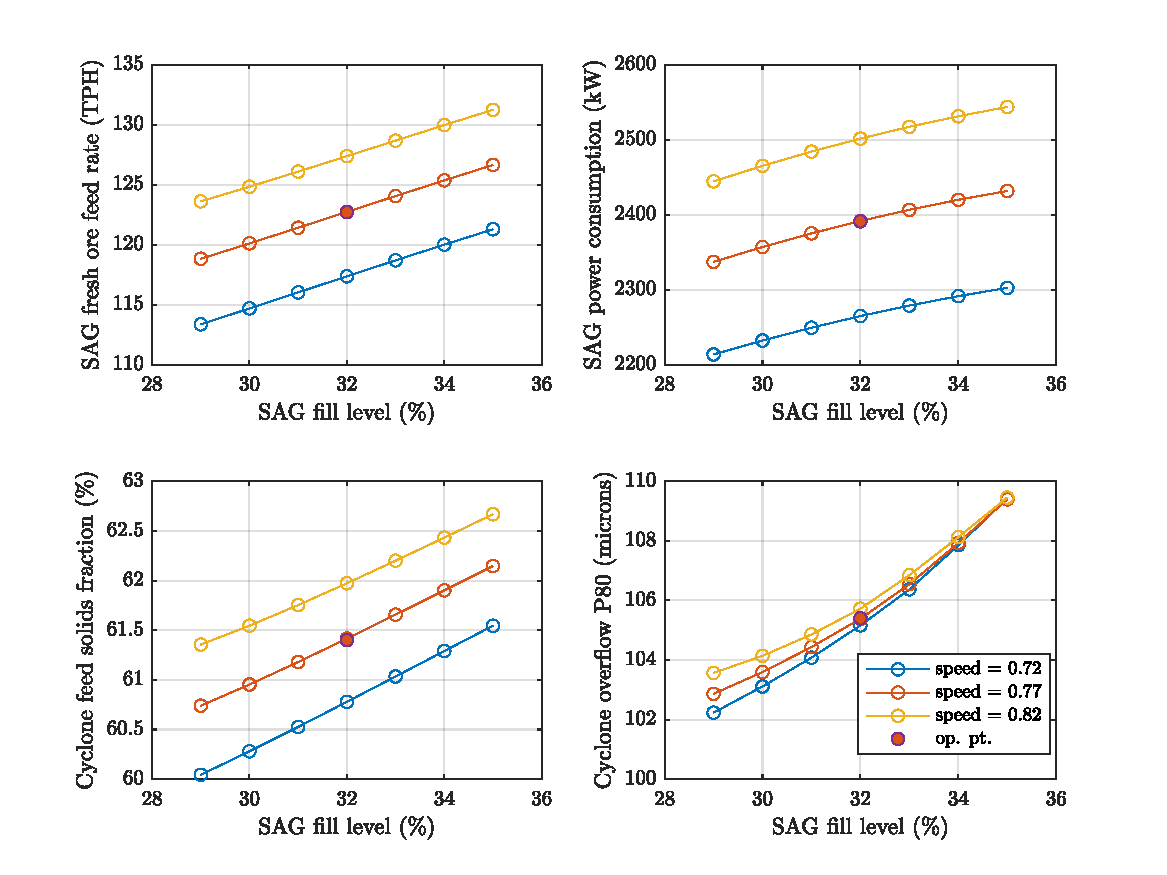
\includegraphics[width=15cm]{images/grind_sim_ss_plot1.pdf}
%	\caption{Steady-state operating points}
%	\label{fig:grind_sim_ss_plot1}
%\end{figure}
%
%\begin{figure}[ht]
%	\centering
%	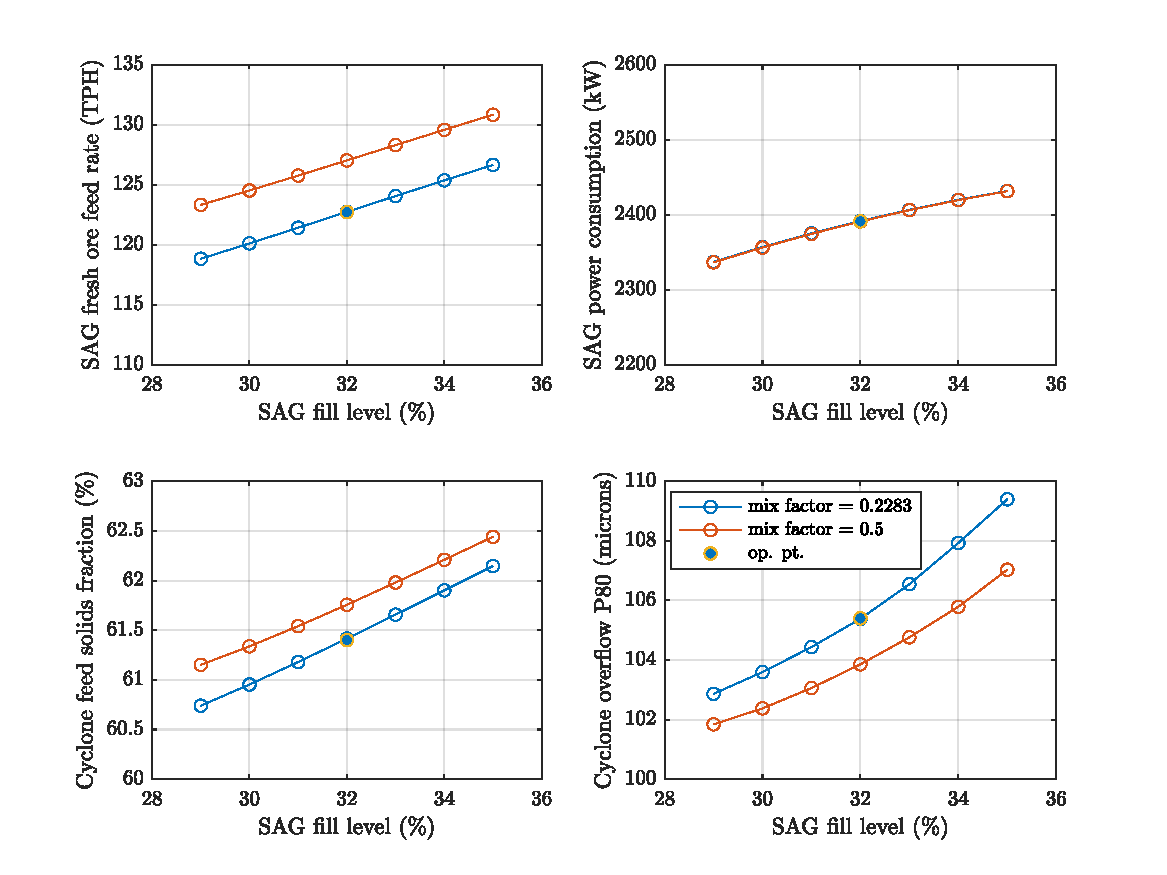
\includegraphics[width=15cm]{images/grind_sim_ss_plot2.pdf}
%	\caption{Effect of ore mix factor on steady-state operating points}
%	\label{fig:grind_sim_ss_plot2}
%\end{figure}

%Zero-mean Gaussian measurement noises are added to the outputs of the simulation model to simulate measurement errors. The standard deviations of these noises are shown in Table \ref{tb:meas-noise}. Except for the measurement noises and the input disturbance described above, the model itself is deterministic.

% Scaling factors
% 2
%& 0.0085
%& 0.01
%& 0.01
%& 2.2
%& 24
%& 0.2
%& 2
%
%\begin{table}[h!]
%	\centering
%	\caption{Simulated output measurements} \label{tb:meas-noise}
%	\begin{tabular}{c >{\raggedright}p{5.5cm} c c}
%		Label & Description & Sampling period (hours) & Noise std. dev. \\
%		\midrule
%		CV1        & Mill weight & 0.05 & XX \\ 
%		CV2       & Mill power consumption & 0.05 & XX \\ 
%		CV3       & Cyclone feed solids fraction & 0.05 & XX \\ 
%		CV4       & Cyclone overflow P80 & 0.05 & XX \\ 
%		\bottomrule
%	\end{tabular}
%\end{table}
%
%
%Although some of these process variables would likely be sampled at higher rates in practice, it is assumed, for simplicity, that they are all sampled at the same rate of 1 sample every 3 minutes (i.e. a sampling period of 0.05 hours). This was deemed to be a typical sampling rate of a standard online particle size analyser that might be used for the P80 measurement.


\section{Performance evaluation} \label{sec:evaluation}

Various metrics are used in this work to evaluate the performance of the observers. Since a simulation model of the plant is used and the input disturbances are also simulated, the true values of the system inputs and outputs (i.e. without measurement errors) are available.

The first metric is the \textit{\acrlong{RMSE}} (\acrshort{RMSE}) of the system output estimates, which is an indication of the magnitude of the differences between the estimates of an output signal, $\hat{Y}_i(N)=\left\{\hat{y}_i(1),\hat{y}_i(2), ..., \hat{y}_i(N)\right\}$, and its true values, $Y_i(N)=\left\{y_i(1),y_i(2), ..., y_i(N)\right\}$, (i.e. the output estimation errors),
\nomenclature{$\hat{Y}_i(k)$}{estimates of system output $i$ from time 0 to time $k$}%
\nomenclature{$\hat{\mathbf{Y}}(k)$}{system output estimates from time 0 to time $k$}%
\nomenclature{$Y_{i}(k)$}{system output $i$ from time 0 to time $k$}%
\nomenclature{$Y_{M,i}(k)$}{measurements of system output $i$ from time 0 to time $k$}%
\nomenclature{$\mathrm{RMSE}(\hat{Y},Y)$}{\acrlong{RMSE} of the output estimates, $\hat{Y}(N)$, from a simulation, compared to the true system outputs, $Y(N)$}%
\nomenclature{$\mathrm{RMSE}(\hat{Y},Y_M)$}{\acrlong{RMSE} of the output estimates, $\hat{Y}(N)$, from a simulation, compared to the system output meaurements, $Y_M(N)$}%
\begin{equation} \label{eq:rmse-calc-yest}
	\newcommand{\RMSE}{\textrm{RMSE}}
	\RMSE(\hat{Y}_i(N),Y_i(N)) = \sqrt{\frac{1}{N}\sum_{k=1}^{N}{(\hat{y}_i(k)-y_i(k))^2}}.
\end{equation}

Similarly, the \gls{RMSE} of the estimates of an unmeasured input disturbance signal, $\hat{p}_i(k)$, is
\begin{equation} \label{eq:rmse-calc-pest}
	\newcommand{\RMSE}{\textrm{RMSE}}
	\RMSE(\hat{P}_i(N),P_i(N)) = \sqrt{\frac{1}{N}\sum_{k=1}^{N}{(\hat{p}_i(k)-p_i(k))^2}}.
\end{equation}
 
As well as the overall \gls{RMSE}, two additional metrics are used to evaluate observer performance on systems with \gls{RODD}s. The \gls{RMSE} \textit{in transition}, which is the \gls{RMSE} during a period after a random shock, is used to evaluate the response of an observer to infrequent, abrupt disturbances. The transition period is defined as the samples occurring within $t_{\pm5\%}$ hours of the disturbance arriving at the input to the process, where $t_{\pm5\%}$ is the \textit{settling time} \hl{of the process}, defined as the time taken for the outputs to converge to within $\pm5\%$ of the final steady-state values. The \gls{RMSE} \textit{in steady-state} is defined as the samples occurring more than $t_{\pm5\%}$ hours after a disturbance and before the next one occurs.
\nomenclature{$t_{\pm5\%}$}{settling time of the process to within $\pm5$ percent of steady-state}%

The fourth metric is the \textit{\acrlong{RMSD}} (\acrshort{RMSD}) in the estimates,
\nomenclature{$\mathrm{RMSD}(\hat{Y})$}{\acrlong{RMSD} of the output estimates, $\hat{Y}(N)$, from a simulation}%
\begin{equation} \label{eq:rmsd-calc-yest}
	\newcommand{\RMSD}{\textrm{RMSD}}
	\RMSD(\hat{Y}_i(N)) = \sqrt{\frac{1}{N}\sum_{k=1}^{N}{(\hat{y}_i(k)-\hat{y}_i(k-1))^2}}.
\end{equation}
\nomenclature{$\mathrm{Var}(\hat{Y})$}{Variance of the output estimates, $\hat{Y}(N)$, from a simulation}%

This is a measure of the magnitude of high frequency changes in the estimates, which is an indication of the sensitivity of an observer to measurement noise.

\hl{A fifth metric is used in the case of the grinding simulator experiments, the variance of the estimates during steady-state periods. This is similar to the {\gls{RMSE}} in that it gives an indication of the sensitivity of the estimates to measurement noise.}
% Variance calc - only used in grinding model simulations
\begin{equation} \label{eq:var-calc}
	\begin{aligned}
		\newcommand{\Var}{\textrm{Var}} 
		\Var(\hat{y}(k)) = \frac{1}{N}\sum_{k=1}^{N}{(\hat{y}(k)-\mu_y)^2} \\
		\mu_y = \frac{1}{N}\sum_{k=1}^{N}{\hat{y}(k)}
	\end{aligned}
\end{equation}

To simplify notation, the argument $N$, indicating the length of the time series, is not always shown. Thus, $\textrm{RMSE}(\hat{Y}_i(N),Y_i(N))$ may be denoted $\textrm{RMSE}(\hat{Y}_i,Y_i)$. The capitalization of $Y$ indicates that it is a time series. Also, for \gls{SISO} systems, the subscript $i$ is redundant and dropped. Thus, $\textrm{RMSE}(\hat{Y},Y)$ is the \gls{RMSE} of the output of a system with only one output variable. However, $\textrm{RMSE}(\hat{\mathbf{Y}},\mathbf{Y})$ is used for a system with more than one output. The assumption is that this is the \gls{RMSE} averaged over all output signals, $Y_i(N)$ for $i=1, ..., n_y$.
% Removed since not doing control simulations.
%To evaluate the potential benefits of the observers in process control applications, simulations were carried out with an observer, a simulated controller, and the simulated process in closed-loop. In these cases, the \gls{RMSE}s of the control variables, $y_i(k)$, compared to a set of reference values, $R_i(N)$, is calculated to evaluate the performance of the control system,
%\begin{equation} \label{eq:rmse-calc-y}
%	\newcommand{\RMSE}{\textrm{RMSE}}
%	\RMSE(Y_i(N),R_i(N)) = \sqrt{\frac{1}{N}\sum_{k=1}^{N}{(y_i(k)-r_i(k))^2}}.
%\end{equation}
%
%In addition, the RMSD of the control actions, $u_i(k)$, is calculated to provide an indication of the sensitivity of the control system to measurement noise,
%\begin{equation} \label{eq:rmsd-calc-u}
%	\newcommand{\RMSD}{\textrm{RMSD}}
%	\RMSD(U_i(N)) = \sqrt{\frac{1}{N}\sum_{k=1}^{N}{(u_i(k)-u_i(k-1))^2}}.
%\end{equation}

Because the processes simulated in this work are stochastic, it is important to evaluate state estimators over sufficiently long simulation time periods to ensure that the results are close to the true average performance and are independent of the specific pseudo-random inputs generated for each simulation. This is particularly important when evaluating systems with \gls{RODD}s because the shocks occur infrequently. As an added precaution, identical random inputs are used when comparing the performance of two or more observers on the same system.

\hljb{In this chapter, the main methods and notation used in this work were introduced. The main disturbance model considered is the {\gls{RODD}} model ({\ref{eq:RODD}}), however, two additional disturbance models were presented, a more general switching model based on the HMM ({\ref{eq:MJLS}}) and the {\gls{BRW}} ({\ref{eq:brw}}). The standard Kalman filter (filtering form) was introduced, along with the multiple-model Kalman filter for estimation of switching systems. The two main sub-optimal algorithms used for {\gls{RODD}} estimation are a sequence fusion algorithm} {\citep{robertson_detection_1995, robertson_method_1998}} \hljb{(two versions of it), and a sequence pruning algorithm} {\citep{eriksson_classification_1996}}, \hljb{with implementation details. The grinding simulation model used to simulate a realistic grinding circuit was also introduced. Finally, the metrics used to evaluate the performance of observers were defined. The next chapter describes a series of simulations carried out to evaluate these observers.}% !TEX encoding = UTF-8 Unicode
\chapter{Methods}
\label{chap-methods}

\section{Disturbance models}

\subsection{Randomly-occurring deterministic disturbances} \label{sec:RODD}

\Acrlong{RODD}s (\acrshort{RODD}s) \citep{macgregor_duality_1984} are a family of stochastic process models suitable for simulating various types of infrequently-occurring disturbances in discrete-time.  The structure of the \gls{RODD} model is
\begin{equation} \label{eq:RODD}
	p(k) = \frac{B(q^{-1})}{A(q^{-1})} w_p(k),
\end{equation}
where $p(k)$ is the generated disturbance signal, $A(q^{-1})$ and $B(q^{-1})$ are polynomial functions of the backward shift operator, $q^{-1}$, and $w_p(k)$ is a random variable generated by a switching system.
\nomenclature{$p(k)$}{disturbance signal at time $k$}%
\nomenclature{$q^{-1}$}{backward shift operator}%
\nomenclature{$A(q^{-1})$}{\acrshort{RODD} model parameter: polynomial function of the backward shift operator}%
\nomenclature{$B(q^{-1})$}{\acrshort{RODD} model parameter: polynomial function of the backward shift operator}%
\nomenclature{$w_p(k)$}{random shock signal at time $k$}%
% One way to make links: \hyperlink{sym.pk}{$p(k)$}.

To generate randomly-occurring disturbances, the switching system,
\begin{equation} \label{eq:wpk1} 
	w_p(k) \sim 
	\begin{cases*}
		0 & with probability $1-\varepsilon$, \\
		\mathcal{N}\left( 0, \sigma_{w_p}^2 \right) & with probability $\varepsilon$,
	\end{cases*}
\end{equation}
\nomenclature{$\varepsilon$}{\acrshort{RODD} model parameter: probability of a random shock}%
may be used, where $w_p(k)$ is either 0 or is sampled from the normal distribution, $\mathcal{N}(0,\sigma_{w_p}^2)$, with mean zero and variance $\sigma_{w_p}^2$.  When the probability $\varepsilon$ is low ($\varepsilon<<1$), this system produces infrequent shocks.
\nomenclature{$\mathcal{N}(\mu,\sigma^2)$}{normal distribution with mean $\mu$ and variance $\sigma^2$}%

Alternatively, a mixture of two distributions may be used \citep{robertson_detection_1995}:
\begin{equation} \label{eq:wpk2}
w_p(k) \sim 
	\begin{cases*}
		\mathcal{N}\left(0, \sigma_{w_p}^2\right) & with probability $1-\varepsilon$, \\
		\mathcal{N}\left(0, b^2\sigma_{w_p}^2\right) & with probability $\varepsilon$.
	\end{cases*}
\end{equation}
\nomenclature{$\sigma_{w_p}$}{\acrshort{RODD} model parameter: standard deviation of the persistent noise component of the random shock variable}%
\nomenclature{$b$}{\acrshort{RODD} model parameter: variance of the random shocks divided by the variance of the persistent noise}%
% Don't think this is necessary to define:
%\nomenclature{$\sigma_{w_p}^2$}{variance of the persistent noise component of the random shock variable}%

In this formulation, $\sigma_{w_p}$ represents the standard deviation of the \hl{persistent} noise in periods between random shocks and $b$ is typically large so that the magnitude of the shocks is many times greater than $\sigma_{w_p}$. One benefit of \eqref{eq:wpk2} is that the distribution of $w_p(k)$ is conditionally Gaussian, whereas in \eqref{eq:wpk1} it has a non-smooth (i.e. degenerate) probability density function.

Figure \ref{fig:wpk-pdf} illustrates the probability density of $w_p(k)$ in the case of \eqref{eq:wpk2} with $\sigma_{w_p}=0.01$, $b=100$, and $\varepsilon=0.01$. Although it is difficult to discern from the plot, this is a mixture distribution with two components. The component that generates the infrequent shocks is barely visible because of its low probability. In this example, 99 percent of the probability lies within a narrow range ($-0.036 < w_p(k) < 0.036$). However, the shocks, which occur with probability 0.01, have much higher amplitude ($b\sigma_{w_p}=1$).

\begin{figure}[ht]
	\centering
	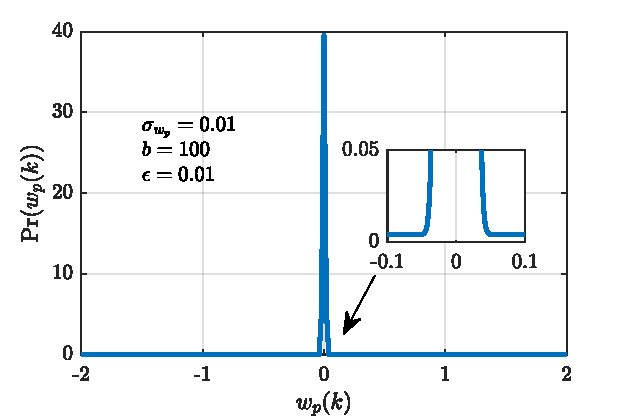
\includegraphics[width=11.5cm]{wpk-pdf-4.pdf}
	\caption{Probability density of a random shock signal}
	\label{fig:wpk-pdf}
\end{figure}

When dealing with a system having more than one \gls{RODD}, where each random shock is independent, the notation is
\begin{equation} \label{eq:wpik2}
	w_{p,i}(k) \sim 
	\begin{cases*}
		\mathcal{N}\left(0, \sigma_{w_p,i}^2\right) & with probability $1-\varepsilon_i$, \\
		\mathcal{N}\left(0, b_i^2\sigma_{w_p,i}^2\right) & with probability $\varepsilon_i$,
	\end{cases*}
\end{equation}
where $i \in \left\{1, 2, ..., n_p\right\}$.
\nomenclature{$n_p$}{number of independent random shock disturbance processes}%

The choice of $A(q^{-1})$ and $B(q^{-1})$ in \eqref{eq:RODD} determines the nature of the \gls{RODD}. For example, if $B(q^{-1})=1$ and $A(q^{-1})=1-q^{-1}$, $p(k)$ will be a random-walk process with infrequent, large step changes.

% Add symbol to glossary
Using $\nabla$ to denote $1-q^{-1}$, the \gls{RODD} \textit{step-disturbance} process can be defined as
\nomenclature{$\nabla$}{defined as $1-q^{-1}$}%
\begin{equation} \label{eq:RODD-step}
	p(k) = \frac{1}{\nabla}w_p(k).
\end{equation}

A \gls{RODD} \textit{ramp-disturbance}, consisting of a series of ramps with randomly-occurring changes in slope, may be generated using
\begin{equation} \label{eq:RODD-ramp}
	p(k) = \frac{1}{\nabla^2}w_p(k).
\end{equation}

A \gls{RODD} consisting of randomly-occurring decaying exponential changes may be generated using
\begin{equation} \label{eq:RODD-exp}
	p(k) = \frac{1}{(1-a_1q^{-1})\nabla}w_p(k),
\end{equation}
where  $0<a_1<1$. Note that $a_1=0$ corresponds to the case of a \gls{RODD} step disturbance \eqref{eq:RODD-step} and $a_1=1$ to that of a \gls{RODD} ramp disturbance \eqref{eq:RODD-ramp}. 

An equivalent state-space representation of \eqref{eq:RODD-exp} is
\begin{equation} \label{eq:RODD-ss}
	\begin{split}
		\mathbf{x}_p(k+1) & =\left[\begin{array}{cc}
			1 & 1 \\
			0 & a_1
		\end{array}\right] \mathbf{x}_p(k) +\left[\begin{array}{cc}
			0 \\
			1
		\end{array}\right] w_p(k) \\
		p(k) & =\left[\begin{array}{cc}
			1 & 0
		\end{array}\right] \mathbf{x}_p(k),
	\end{split}
\end{equation}
\nomenclature{$\mathbf{x}_p(k)$}{disturbance model states at time $k$}%
where $\mathbf{x}_p(k) \in \mathbb{R}^2$ is the state vector.

A disturbance with a combination of different \gls{RODD}s is also possible.  For example, a state-space representation of a \gls{RODD} consisting of step changes and ramps is
\begin{equation} \label{eq:RODD-step-ramp}
	\begin{split}
		\mathbf{x}_p(k+1) & =\left[\begin{array}{cc}
			1 & 1 \\
			0 & 1
		\end{array}\right] \mathbf{x}_p(k) +\left[\begin{array}{cc}
			1 & 0 \\
			0 & 1
		\end{array}\right] \mathbf{w}_p(k) \\
		p(k) & =\left[\begin{array}{cc}
			1 & 0
		\end{array}\right] \mathbf{x}_p(k),
	\end{split}
\end{equation}

where $\mathbf{w}_p(k)$ is a vector of two independent random shock signals generated by \eqref{eq:wpik2}. Simulated examples of these \gls{RODD}s are presented in figures \ref{fig:rodd-sim-plots} and \ref{fig:rodd-sim-plot2}.

\subsection{Hidden Markov models} \label{sec:HMM}

\textit{Hidden Markov models} (\gls{HMM}) can be used to simulate a more diverse set of switching behaviours than those of the \gls{RODD} model described in the previous section \citep{wong_realistic_2009}. A Markov process or Markov chain is a stochastic model used to describe a sequence of discrete events for which the probability of future events depends only on the current state. A \gls{HMM} is a Markov model with states that are not fully observable (i.e. hidden or observed with a measurement error).

To illustrate the basic concept, the state of the random shock process \eqref{eq:wpk2} \hl{may be defined} as a Markov model with a state that has two possible values,
\begin{equation} \label{eq:gamma-k}
	\gamma(k) \in \{0,1\}.
\end{equation}
\nomenclature{$\gamma(k)$}{random shock indicator at time $k$}%
$\gamma(k)=1$ represents a shock at time $k$, and $\gamma(k)=0$ means no shock occurs. The switching of $\gamma(k)$ can then be defined by a \textit{transition matrix}, $\Pi$, which describes the probabilities of transitioning from every mode at time $k$ to every mode at time $k+1$:
\begin{equation} \label{eq:Pi}
	\begin{aligned}
	\Pi &= \left(\pi_{ij} \forall i,j\in \{1,2,...,n_j\}\right) \\
	\pi_{ij} &= \Pr\left( \gamma(k)=j-1 \mid \gamma(k-1)=i-1 \right),
	\end{aligned}
\end{equation}
\nomenclature{$\Pr(A \mid B)$}{probability of an event $A$ given an event $B$}%
\nomenclature{$n_j$}{number of modes or models of a switching system}%
where $n_j$ is the number of possible system modes and $\pi_{ij}$ is the probability that the system mode at time $k$ is $j-1$ given that it was $i-1$ at time $k-1$.

In the case of the random shock, $n_j=2$ and the equivalent Markov process has the transition probability matrix
\nomenclature{$\Pi_{w_{p}}$}{transition probability matrix of the disturbance process $w_p$}%
\begin{equation} \label{eq:Pi-RODD-step}
	\Pi_{w_{p}} = \begin{bmatrix}
	1-\varepsilon & \varepsilon \\
	1-\varepsilon & \varepsilon
	\end{bmatrix}.
\end{equation}
Since $w_{p}(k)$ is an independent random variable, it does not depend on the previous state, $\gamma(k-1)$. Therefore, the rows of $\Pi_{w_{p}}$ are identical.

The use of the Markov model thus allows transition probabilities that do depend on the previous state. For example, consider a disturbance where the signal switches infrequently between samples from two or more distributions with different parameters. The probabilities of switching from one distribution to another may be different. Such a disturbance process could be simulated with a hidden Markov model by conditioning the distribution from which $w_p(k)$ is sampled on a Markov state, $r(k)$, with an arbitrary number of modes,
\nomenclature{$r(k)$}{mode indicator of a switching system at time $k$}%
\begin{equation} \label{eq:mog-example}
	\begin{split}
		w_p(k) \sim 
		\begin{cases*}
			\mathcal{N}\left(\mu_{w_p,1}, \sigma_{w_p,1}\right) & if $r(k)=1$, \\
			\mathcal{N}\left(\mu_{w_p,2}, \sigma_{w_p,2}\right) & if $r(k)=2$, \\
			... & ...\\
			\mathcal{N}\left(\mu_{w_p,n_j}, \sigma_{w_p,n_j}\right) & if $r(k)=n_j$.
		\end{cases*} \\
	\Pr(r(k)=j-1 \mid r(k-1)=i-1)=\pi_{ij} \forall i,j \in {1,2,...,n_j}
	\end{split}
\end{equation}

To make the notation more concise, allow the value of any time-varying discrete variable such as $\sigma_{w_p} \in \left\{\sigma_{w_p,1}, \sigma_{w_p,2},..., \sigma_{w_p,n_j}\right\}$, to be determined by the value of the Markov state $r(k)$. Thus,
\begin{equation} \label{eq:A-selection}
	\sigma_{w_p}(r(k)) = 
	\begin{cases*}
		\sigma_{w_p,1} & if $r(k)=1$, \\
		\sigma_{w_p,2} & if $r(k)=2$, \\
		... & ...\\
		\sigma_{w_p,n_j} & if $r(k)=n_j$.
	\end{cases*}
\end{equation}

With this notation, \eqref{eq:mog-example} can be written concisely as
\begin{equation} \label{eq:mog-example2}
	\begin{aligned}
		w_p(k) &\sim \mathcal{N}\left(\mu_{w_p}(r(k)), \sigma_{w_p}(r(k))\right) \\
		\Pr(r(k) &= j-1 \mid r(k-1)=i-1)=\pi_{ij} \forall i,j \in {1,2,...,n_j}.
	\end{aligned}
\end{equation}
where $\mu_{w_p}\in\left\{\mu_{w_p,1},\mu_{w_p,2},...,\mu_{w_p,n_j}\right\}$. This model is known as a \textit{mixture of Gaussians} and can be considered a special-case of a HMM-based disturbance model \citep{wong_disturbance_2007}.

A \gls{HMM} disturbance process can be represented by a \textit{Markov jump linear system} (\acrshort{MJLS}) \citep{costa_discrete-time_2005}. The state-space representation with time-varying system matrices $\mathbf{A}(\gamma(k))$, $\mathbf{B}(\gamma(k))$, and $\mathbf{C}(\gamma(k))$, and a vector of independent time-varying random shock inputs, $\mathbf{w}_p(k)$ \eqref{eq:mog-example2}, is defined
\begin{equation} \label{eq:MJLS}
	\begin{aligned}
	\mathbf{x}_p(k+1) &= \mathbf{A}(r(k)) \mathbf{x}_p(k) + \mathbf{B}(r(k))\mathbf{w}_p(k) \\
	\mathbf{p}(k) &= \mathbf{C}(r(k)) \mathbf{x}_p(k) + \mathbf{e}_p(k).
	\end{aligned}
\end{equation}

Note that $\mathbf{e}_p(k)$ may also be a switching random variable if desired. \eqref{eq:MJLS} is a versatile model suitable for representing and simulating a diverse family of stochastic disturbances.

\subsection{Bounded disturbances} \label{sec:bounded}

The \textit{bounded random walk} (\gls{BRW}) is a stochastic process proposed by \cite{nicolau_stationary_2002}. The discrete-time version is defined by the difference equation
\begin{equation} \label{eq:brw}
		p(k+1) = p(k) + a(p(k)) + e(k),
\end{equation}
where $e(k)$ is a random noise with variance $\sigma_e^2$, and $a(\cdot)$ is a function defined as
\nomenclature{$a(\cdot)$}{additive bias function used in the \acrshort{BRW}}%
\nomenclature{$\alpha_{1}$}{\acrshort{BRW} parameter}%
\nomenclature{$\alpha_{2}$}{\acrshort{BRW} parameter}%
\nomenclature{$\tau$}{\acrshort{BRW} parameter}%
\begin{equation}
	a(x) = e^{\beta}\left(e^{-\alpha_{1}\left(x - \tau\right)} - e^{\alpha_{2}\left(x - \tau\right)}\right),
\end{equation}
where $\beta$, $\alpha_{1}$, and $\alpha_{2}$ are constants.  From \eqref{eq:brw} it can be deduced that
\begin{equation}
	\mathbb{E}\{p(k+1)|p(k)\} = p(k) + a(p(k)).
\end{equation}

Therefore, $a(p(k))$ has the effect of an additive bias or time-varying adjustment to $p(k+1)$ that depends on $p(k)$. The shape of $a(\cdot)$ is determined by the constants $\alpha_{1}$,  $\alpha_{2}$, $\beta$, and $\tau$. Figure \ref{fig:brw-a} shows $a(p(k))$ in the case where $\tau=100$, $\beta=-15$, and $\alpha_{1}=\alpha_{2}=3$.  From this, it is clear that in the vicinity of $p(k)=\tau$, $a(p(k))\approx0$. When $a(p(k))=0$, \eqref{eq:brw} is the equation for a random walk. However, outside the neighbourhood, $p(k) \approx \tau$, $a(p(k))$ increases for low $p(k)$ or decreases for high $p(k)$. This has the effect of causing $p(k+1)$ to revert towards the mean ($\tau$) whenever $p(k)$ strays outside the neighbourhood. 
\begin{figure}[ht]
	\centering
	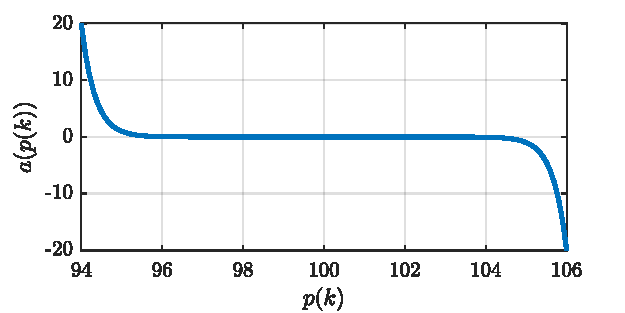
\includegraphics[height=5cm]{images/brw_a.pdf}
	\caption{A bounded random walk bias function}
	\label{fig:brw-a}
\end{figure}

Figure \ref{fig:brw-sim} shows a simulation of a \gls{BRW} with the above parameter values, and for comparison, an unbounded random walk (labelled `RW') generated with the same noise input. The dashed lines at $p(k)=95$ and $p(k)=105$ roughly indicate the location of the lower and upper bounds, which the \gls{BRW} only marginally exceeds.
\begin{figure}[ht]
	\centering
	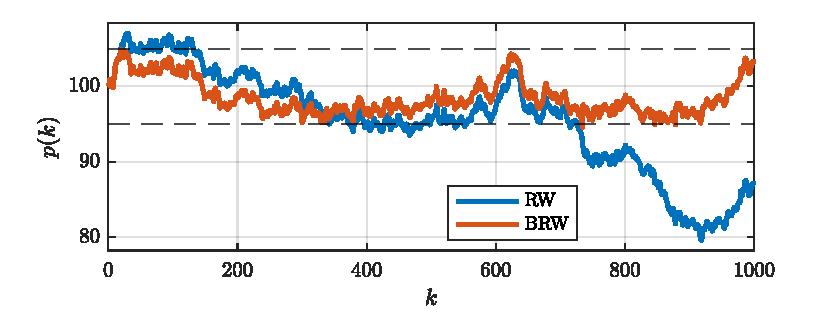
\includegraphics[height=5cm]{images/brw_sim.pdf}
	\caption{Examples of a bounded and unbounded random walk}
	\label{fig:brw-sim}
\end{figure}

Unlike a simple random walk, the \gls{BRW} is stationary. \cite{nicolau_stationary_2002} derived a formula for the form of the unconditional (i.e. stationary) probability distribution of the continuous-time \gls{BRW}. Figure \ref{fig:brw-pdf} shows the normalized stationary probability density of the \gls{BRW} defined above. For comparison, the probability density of a random walk process after 20 sample periods is also shown. It can be seen that there is a significant probability that the random walk would exceed the bounds of this \gls{BRW} after 20 sample periods. It can also be seen that the central part of the probability distribution of the \gls{BRW} is flat, indicating that all values within the bounds are equally likely after a large number of samples, similar to a uniform probability distribution.

%\begin{equation}
%	p_{BRW}(x) \propto \sigma^{-2} \exp \left\{-\frac{2 e^{k}}{\sigma^{2}}\left(\frac{e^{-\alpha_{1}(x-\tau)}}{\alpha_{1}}+\frac{e^{\alpha_{2}(x-\tau)}}{\alpha_{2}}\right)\right\}
%\end{equation}

\begin{figure}[ht]
	\centering
	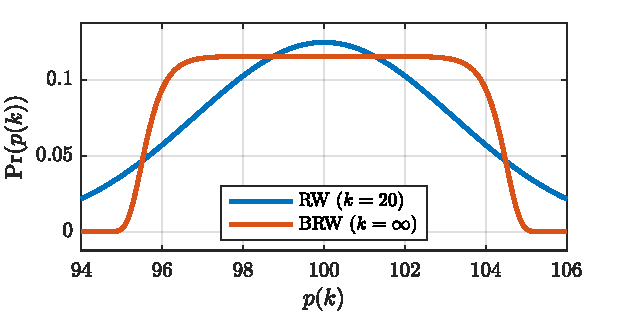
\includegraphics[height=5cm]{images/brw_pdf.pdf}
	\caption{Probability distributions of bounded and unbounded random walks}
	\label{fig:brw-pdf}
\end{figure}

However, the \gls{BRW} as defined in \eqref{eq:brw} is not guaranteed to be stable. Extreme values of $p(k)$ may cause $|a(p(k))|$ to be greater than $2|p(k)|$, which results in rapid divergence. This would cause computational errors in a numerical simulation. To avoid this, \cite{nicolau_stationary_2002} recommends adding a conditional regularizing step that forces reversion towards the mean, $\tau$, when the correction bias is too large. Instead of \eqref{eq:brw}, a conditional difference equation,
\begin{equation} \label{eq:brw-reg}
	p(k+1) = \begin{cases*}
		p(k) + a(p(k)) + e(k) & if $\left|a(p(k)) \right| < 2\left| p(k) - \tau \right|$, \\
		\tau + \phi(p(k) - \tau) + e(k) & if $\left|a(p(k)) \right| \geq 2\left| p(k) - \tau \right|$,
	\end{cases*}
\end{equation}
is used, where $\phi$ is a constant such that $0<\phi<1$. The size of $\phi$ determines how fast $p(k)$ reverts to $\tau$ when it is outside the stable region.

Since the \gls{BRW} has a non-Gaussian probability distribution, analysis of the properties of any dynamical system with a \gls{BRW} input is difficult. However, for simulation purposes, the \gls{BRW} is a simple and practical solution to the problem of bounding a random disturbance.

The \gls{BRW} concept could be extended to \gls{RODD}s. A \gls{RODD} step disturbance \eqref{eq:RODD-step} is a random walk with a switching noise variance \eqref{eq:wpk2}. The concern when trying to bound such a disturbance is the large step changes that occur infrequently. Since the probability of the shock, as well as the sign and amplitude of the step, are independent random variables, a \gls{RODD} step disturbance that happens to be at one of the bounds is as likely to step outside the bound as it is to step back inside the bounded region. The conditional regularity used in the \gls{BRW} \eqref{eq:brw-reg} would prevent any computational problems.


\section{State estimation} \label{sec:estimation}

State estimation is the task of estimating the values of the state variables of a dynamic model of a system given a set of measurements from the system. In process control applications, estimates of the states at the current time, or a prediction of their values at the next time instant, are required in real time (i.e. online) in order to calculate an appropriate control action.

Consider the diagram of an input-output system model in Figure \ref{fig:model_diag_uwvy}. Here, $\mathbf{u}(k)$ $\in \mathbb{R}^{n_u}$ is a vector of known input variables at time instant $k$, $\mathbf{w}(k)$ $\in \mathbb{R}^n$ is a vector of unmeasured state disturbances, $\mathbf{v}(k) \in \mathbb{R}^{n_y}$ is a vector of measurement errors, and $\mathbf{y}_M(k) \in \mathbb{R}^{n_y}$ is a vector of output measurements. The box represents a mathematical model that relates the inputs to the outputs and may be time-varying.
\nomenclature{$\mathbf{u}(k)$}{system inputs at time $k$}%
\nomenclature{$\mathbf{y}(k)$}{system outputs at time $k$}%
\nomenclature{$\mathbf{w}(k)$}{process disturbances at time $k$}%
\nomenclature{$\mathbf{v}(k)$}{measurement noises at time $k$}%
\begin{figure}[ht]
	\centering
	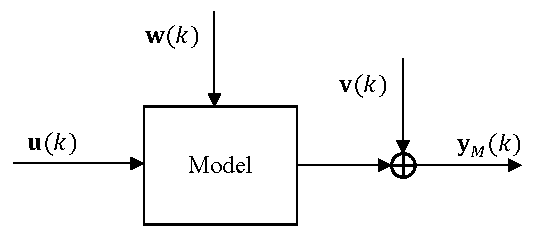
\includegraphics[width=8cm]{images/model_diag_uwvy.pdf}
	\caption{System model diagram}
	\label{fig:model_diag_uwvy}
\end{figure}

A convenient form in which to represent discrete-time, linear, possibly time-varying, dynamical system models for state estimation and control purposes, is the state-space representation
\begin{equation} \label{eq:ss_rep_uwy}
	\begin{aligned}
		\mathbf{x}(k+1) &= \mathbf{A}(k) \mathbf{x}(k) + \mathbf{B}(k) \mathbf{u}(k) + \mathbf{w}(k), \\
		\mathbf{y}_M(k) &= \mathbf{C}(k) \mathbf{x}(k) + \mathbf{v}(k).
	\end{aligned}
\end{equation}
\nomenclature{$\mathbf{x}(k)$}{system model states at time $k$}%
\nomenclature{$\mathbf{A}$}{transition matrix of the system model}%
\nomenclature{$\mathbf{B}$}{input matrix of the system model}%
\nomenclature{$\mathbf{C}$}{output matrix of the system model}%
where $\mathbf{x}(k)$ $\in \mathbb{R}^n$ is a vector of state variables, $\mathbf{A}(k) \in \mathbb{R}^{n \times n}$ is the state transition matrix at time $k$, $\mathbf{B}(k) \in \mathbb{R}^{n \times n_u}$ is the input matrix at time $k$, and $\mathbf{C}(k) \in \mathbb{R}^{n_y \times n}$ is the output matrix at time $k$. In this work, the system matrices are not time-varying and are therefore denoted $\mathbf{A}$, $\mathbf{B}$, and $\mathbf{C}$ in the remainder of this chapter.

The \textit{Kalman filter} \citep{kalman_new_1960} is the optimal estimator for a linear system in which the unmeasured disturbances and measurement errors are Gaussian random variables with mean values of zero. There are two commonly-used implementations of the Kalman filter, the \textit{prediction form} and the \textit{filtering form}. In the prediction form, the estimates of the states at the next time instant ($k+1$), given the information available at the current time ($k$) are calculated using
\begin{equation}
\begin{aligned} \label{eq:xkp1_hat_p}
	\mathbf{\hat{x}}(k+1 \mid k) &= \mathbf{\hat{x}}(k+1 \mid k-1) + \mathbf{K}_p(k) \big( \mathbf{y}_M(k) - \mathbf{\hat{y}}(k \mid k-1) \big) \\
	&= \mathbf{A}\mathbf{\hat{x}}(k \mid k-1) + \mathbf{B}\mathbf{u}(k) + \mathbf{K}_p(k) \big( \mathbf{y}_M(k) - \mathbf{C} \mathbf{\hat{x}}(k \mid k-1) \big)
\end{aligned}
\end{equation}
\nomenclature{$\mathbf{y}_M(k)$}{system output measurements at time $k$}%
where $\hat{\mathbf{x}}(k \mid k-1)$ is the prediction of the states at time $k$ that was made with the information available at the previous time instant, $k-1$, $\mathbf{y}_M(k)$ is the current measurement of the output, and $\mathbf{K}_p(k) \in \mathbb{R}^{n \times n_y}$ is a (possibly time-varying) correction gain.
\nomenclature{$\mathbf{K}_p(k)$}{correction gain of the Kalman filter (prediction form)}%

In the filtering form, which is used in this work, the estimated states and outputs at the current time are calculated given the information available at the current time using
\begin{equation} \label{eq:xkyk_hat}
	\begin{aligned}
		\mathbf{\hat{y}}(k \mid k-1) &= \mathbf{C} \mathbf{\hat{x}}(k \mid k-1) \\
		\mathbf{\hat{x}}(k \mid k) &= \mathbf{\hat{x}}(k \mid k-1) + \mathbf{K}(k) \big( \mathbf{y}_M(k) - \mathbf{\hat{y}}(k \mid k-1)  \big) \\
		\mathbf{\hat{y}}(k \mid k) &= \mathbf{C} \mathbf{\hat{x}}(k \mid k)
	\end{aligned}
\end{equation}
\nomenclature{$\hat{\mathbf{x}}(k \mid k-1)$}{predictions of system model states at time $k$ made with information available at time $k-1$}%
\nomenclature{$\mathbf{K}(k)$}{correction gain of the Kalman filter (filtering form)}%
where $\mathbf{K}(k)$ $\in \mathbb{R}^{n \times n_y}$ is a (possibly time-varying) correction gain. Instead of \eqref{eq:xkp1_hat_p}, the predictions of the states at the next time instant are calculated using
\nomenclature{$\hat{\mathbf{x}}(k+1 \mid k)$}{predictions of system modelstates at time $k+1$ made with information available at time $k$}%
\nomenclature{$\hat{\mathbf{x}}(k \mid k)$}{estimates of system model states at time $k$ made with information available at time $k$}%
\nomenclature{$\hat{\mathbf{y}}(k \mid k)$}{estimates of system outputs at time $k$ made with information available at time $k$}%
\begin{equation} \label{eq:xkp1_hat}
	\mathbf{\hat{x}}(k+1 \mid k) = \mathbf{A} \mathbf{\hat{x}}(k \mid k) + \mathbf{B} \mathbf{u}(k).
\end{equation}

An intuitive interpretation of the Kalman filter is that it takes the predictions of the states at time $k$ made in the previous time instant using the system model, and corrects them based on the difference between the current output measurement, $\mathbf{y}_M(k)$, and the output predicted by the model, $\mathbf{C} \mathbf{\hat{x}}(k \mid k-1)$. The correction step \eqref{eq:xkyk_hat} and prediction step \eqref{eq:xkp1_hat} are executed iteratively each time step, given a prior prediction of the states at time zero, $\mathbf{\hat{x}}(0 \mid -1)=\mathbf{\hat{x}}_0$.
\nomenclature{$\mathbf{\hat{x}}_0$}{Initial values of the estimates of the system states at time 0}%

Although the predicted states, $\hat{\mathbf{x}}(k \mid k-1)$, are identical in both forms of the Kalman filter, the use of the updated (i.e. \textit{a posteriori}) estimates, $\hat{\mathbf{x}}(k \mid k)$, in the filtering form instead of the predicted states leads to an optimal estimate taking account of all the information available. However, it should be noted that in some control applications, the prediction form is beneficial because the state predictions, $\hat{\mathbf{x}}(k+1 \mid k)$, are available one time step ahead.

To track a system with time-varying parameters, a dynamic estimator is needed with a time-varying correction gain. In the case of the filtering form of the Kalman filter, $\mathbf{K}(k)$ is calculated at each time instant using
\begin{equation} \label{eq:Kk}
	\mathbf{K}(k) = \mathbf{P}(k \mid k-1)\mathbf{C}^\intercal \mathbf{S}^{-1}(k),
\end{equation}
where $\mathbf{S}(k)$ is the output prediction error covariance matrix, which is given by
\nomenclature{$\mathbf{S}(k)$}{covariance of the output prediction errors at time $k$}%
\begin{equation} \label{eq:Sk}
	\mathbf{S}(k) = \mathbf{C}\mathbf{P}(k \mid k-1)\mathbf{C}^\intercal + \mathbf{R},
\end{equation}
\nomenclature{$\mathbf{P}(k \mid k-1)$}{predictions of the state estimation error covariance at time $k$ made with information available at time $k-1$}%
and $\mathbf{P}(k \mid k-1)$ is the state estimation error covariance matrix calculated in the previous time instant. $\mathbf{R}$, which is time invariant in this work, is the covariance matrix of the measurement noises,
\nomenclature{$\mathbf{R}$}{covariance of the measurement noises in the observer model}%
\begin{equation} \label{eq:R}
	 \mathbf{R} = \mathbb{E}\{ \mathbf{v}(k) \mathbf{v}^\intercal(k) \},
\end{equation}
\nomenclature{$\mathbb{E}\{\cdot\}$}{expectation operator}%
where $\mathbb{E}\{\cdot\}$ is the expectation operator.

The corrected error covariance may be calculated using
\nomenclature{$\mathbf{P}(k \mid k)$}{state estimation error covariance at time $k$ made with information available at time $k$}%
\begin{equation} \label{eq:Pk}
	\mathbf{P}(k \mid k) = \left( \mathbf{I}_n - \mathbf{K}(k) \mathbf{C} \right) \mathbf{P}(k \mid k-1),
\end{equation}
given an initial covariance estimate at time zero, $\mathbf{P}(0 \mid -1)=\mathbf{P}_0$.%
\nomenclature{$\mathbf{P}_0$}{Initial value of the state estimation error covariance at time 0}

However, to reduce numerical errors due to rounding, the computation of $\mathbf{P}(k \mid k)$ is carried out in this work using the Joseph stabilized version of \eqref{eq:Pk} {\citep{lewis_optimal_2008}
 \begin{equation} \label{eq:Pk-stab}
 	\mathbf{P}(k \mid k) = \left( \mathbf{I}_n - \mathbf{K}(k) \mathbf{C} \right ) \mathbf{P}(k \mid k-1) \left( \mathbf{I}_n - \mathbf{K}(k) \mathbf{C} \right )^\intercal + \mathbf{K}(k)  \mathbf{R} \mathbf{K}(k)^\intercal,
 \end{equation}
\nomenclature{$\mathbf{I}_n$}{the identity matrix ($n \times n$)}%
where $\mathbf{I}_n$ is the identity matrix.

The prediction of the error covariance at the next time instant is made using
\nomenclature{$\mathbf{P}(k+1 \mid k)$}{predictions of the state estimation error covariance at time $k+1$ made with information available at time $k$}%
\begin{equation} \label{eq:Pkp1}
	\mathbf{P}(k+1 \mid k) = \mathbf{A} \mathbf{P}(k \mid k)  \mathbf{A}^\intercal  + \mathbf{Q}(k),
\end{equation}
where $\mathbf{Q}(k)$ is the time-varying covariance of the process disturbances,
\nomenclature{$\mathbf{Q}(k)$}{covariance of the process disturbances in the observer model at time $k$}%
\begin{equation} \label{eq:Q}
	\mathbf{Q}(k) = \mathbb{E}\{ \mathbf{w}(k) \mathbf{w}^\intercal(k) \}.
\end{equation}

Algorithm \ref{alg:kf} defines the sequence of the Kalman filter calculations at each time instant. 
\nomenclature{$\mathcal{Q}$}{set of process noise covariance matrices of a switching system model}%
This is for the case with only the covariance, $\mathbf{Q}(k)$, switching according to the shock indicator, $\gamma(k)$, \eqref{eq:init_Q}. It can easily be extended to simulate other switching model components, such as $\mathbf{R}(k)$, $\mathbf{A}(k)$, $\mathbf{B}(k)$, or $\mathbf{C}(k)$ as defined in \eqref{eq:ss_rep_uwy}. \hl{An alternative to the representation used in this work would be to implement the switching of the random shock {\eqref{eq:wpk2}} using a time-varying input matrix, $\mathbf{B}(k)$, instead of the time-varying prediction error covariance, $\mathbf{Q}(k)$ in {\eqref{eq:Pkp1}}. Both methods are valid and equivalent.}
\begin{algorithm}
	\caption{Kalman filter update}\label{alg:kf}
	%\algorithmfootnote{$y_0$ denotes the initial value.}
	\begin{algorithmic}
		\Require $\mathbf{A},\mathbf{B},\mathbf{C},\mathbf{\hat{x}}(k \mid k-1), \mathbf{P}(k \mid k-1), \mathcal{Q}, \mathbf{R}, \mathbf{\gamma}(k), \mathbf{u}(k), \mathbf{y}_M(k)$
		\State calculate $\mathbf{S}(k)$ \eqref{eq:Sk}
		\State calculate $\mathbf{K}(k)$ \eqref{eq:Kk}
		\State calculate $\mathbf{\hat{x}}(k \mid k)$ and $\mathbf{\hat{y}}(k \mid k)$ \eqref{eq:xkyk_hat}
		\State calculate $\mathbf{P}(k \mid k)$ \eqref{eq:Pk-stab}
		\State calculate $\mathbf{\hat{x}}(k+1 \mid k)$ \eqref{eq:xkp1_hat}
		\State $\mathbf{Q}(k) \gets \mathcal{Q}(\gamma(k))$
		\State calculate $\mathbf{P}(k+1 \mid k)$ \eqref{eq:Pkp1}
	\end{algorithmic}
\end{algorithm}

Also note that in a control application, the manipulated input, $\mathbf{u}(k)$, is computed by the control algorithm. This may be done before the Kalman filter calculations in algorithm \ref{alg:kf} if the prior prediction of the states in the current time instant, $\hat{\mathbf{x}}(k \mid k-1)$, is used. Alternatively, slightly better control performance might be achieved if the control algorithm uses the updated (a-posteriori) state estimates, $\hat{\mathbf{x}}(k \mid k)$. In the latter case, the Kalman filter calculations must be interrupted to compute the control action after the state correction step \eqref{eq:xkyk_hat} and prior to the prediction step \eqref{eq:xkp1_hat}, when $\mathbf{u}(k)$ is needed.

\begin{figure}[ht]
	\centering
	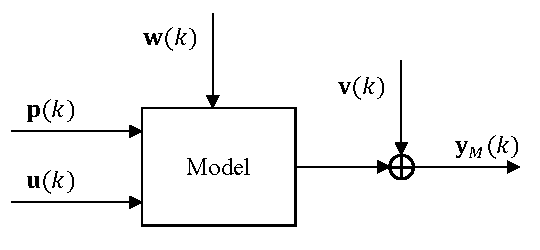
\includegraphics[width=8cm]{images/model_diag_upwvy.pdf}
	\caption{System model with disturbance inputs and manipulated inputs}
	\label{fig:model_diag_upwvy}
\end{figure}
In the case where the system has unmeasured disturbance inputs, $\mathbf{p}(k) \in \mathbb{R}^{n_p}$, as depicted in Figure \ref{fig:model_diag_upwvy}, the state-space equations \eqref{eq:ss_rep_uwy} are modified to include these by splitting the input matrix into two parts, $\mathbf{B}_u \in \mathbb{R}^{n \times n_u}$ and $\mathbf{B}_p \in \mathbb{R}^{n \times n_p}$,
\begin{equation} \label{eq:ss_rep_upwy}
	\begin{aligned}
		\mathbf{x}(k+1) = \mathbf{A} \mathbf{x}(k) + \mathbf{B}_u \mathbf{u}(k) + \mathbf{B}_p \mathbf{p}(k) + \mathbf{w}(k), \\
		\mathbf{y}_M(k) = \mathbf{C} \mathbf{x}(k) + \mathbf{v}(k).
	\end{aligned}
\end{equation}

For state estimation in the presence of unmeasured disturbances, which is always the case in practice, a suitable model of the disturbances is needed. This model is shown in Figure \ref{fig:model_diag_wpupwvy} with a vector of random shock variables, $\mathbf{w}_p(k)$, at its input.
\nomenclature{$\mathbf{w}_p(k)$}{random shock signals at time $k$}%
\begin{figure}[ht]
	\centering
	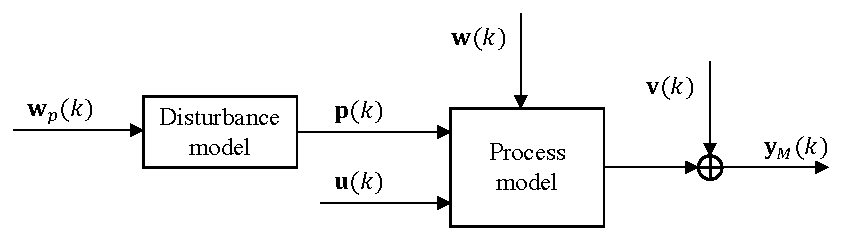
\includegraphics[width=12.5cm]{images/model_diag_wpupwvy.pdf}
	\caption{System with process model and disturbance model}
	\label{fig:model_diag_wpupwvy}
\end{figure}

A state-space representation of the combined system including the disturbance model can be constructed. This is referred to as the \textit{augmented system model},
\begin{equation} \label{eq:ss_rep_xa}
	\begin{aligned}
		\mathbf{x}_a(k+1) = \mathbf{A}_a \mathbf{x}_a(k) + \mathbf{B}_{a,u} \mathbf{u}(k) + \mathbf{B}_{a,w} \mathbf{w}_{a}(k), \\
		\mathbf{y}(k) = \mathbf{C}_a \mathbf{x}_a(k) + \mathbf{v}(k),
	\end{aligned}
\end{equation}
%\nomenclature{$\mathbf{x}_a(k)$}{augmented system states at time $k$}%
where $\mathbf{x}_a(k) \in \mathbb{R}^{n+n_p}$ is an augmented state vector that includes the states of both the process model and the disturbance model, 
\begin{equation} \label{eq:xak}
	\mathbf{x}_a(k) = \begin{bmatrix}
		\mathbf{x}(k) \\
		\mathbf{x}_p(k)
	\end{bmatrix},
\end{equation}
and $\mathbf{w}_a(k) \in \mathbb{R}^{n+n_p}$ is an augmented vector of random variables, including the random shocks,
\begin{equation} \label{eq:wak}
	\mathbf{w}_a(k) = \begin{bmatrix}
		\mathbf{w}(k) \\
		\mathbf{w}_p(k)
	\end{bmatrix}.
\end{equation}

However, note that this notation with subscript `a' is only used in this section. In subsequent sections, the subscript is dropped for simplicity since all references to the system model refer to the augmented model used for state estimation.

Although the random shock in a \gls{RODD} is unmeasured, it may be observable from the measurements of the outputs of the system. As mentioned in Section \ref{detection_RODDs}, systems with \gls{RODD}s pose problems for state estimation using standard Kalman filters due to the switching of the noise model parameters, namely, the variance of $w_p(k)$ \eqref{eq:wpk2}. As explained by \cite{andersson_adaptive_1985}, a trade-off must be made during the filter design between its ability to respond to the infrequent disturbance when it occurs, and its sensitivity to noise at other times.


\subsection{Multiple model approaches} \label{sec:multi-model}

One option for state estimation of switching (i.e. hybrid) systems is the so-called \textit{multiple-model approach}. Multiple-model observers account for different possible hypotheses about the current and past states of the system and infer from these an overall `best' estimate of the current states. To achieve this, an independent Kalman filter is maintained for each hypothesis and a weighted average of the estimates by each filter is calculated using the conditional probabilities of each hypothesis given current and past measurements.

Let the number of hypotheses and Kalman filters be $n_h$ and the \textit{shock mode hypothesis} associated with Kalman filter $f$ at time $k$ be
\nomenclature{$n_h$}{number of hypotheses maintained by a multiple-model observer}%
\begin{equation} \label{eq:gammak}
	\gamma_{f}(k) \in \left\{0, 1 \right\} \forall{k \ge 0}.
\end{equation}

First, consider the case of estimating only one shock signal \eqref{eq:wpk2}. Therefore, $\gamma_f(k)$ is a scalar. The transition probabilities of the random shock are independent of previous shocks:
\nomenclature{$\gamma_f(k)$}{random shock indicator of hypothesis $f$ at time $k$}%
\begin{equation} \label{eq:Pr_gammak_given_gammakm1}
	\begin{aligned}
		& \Pr\left(\gamma_{f}(k)=0 \mid \gamma_{f}(k-1)\right) = \Pr\left(\gamma_{f}(k)=0\right) = 1-\varepsilon, \\
		& \Pr\left(\gamma_{f}(k)=1 \mid \gamma_{f}(k-1)\right) = \Pr\left(\gamma_{f}(k)=1\right) = \varepsilon.
	\end{aligned}
\end{equation}

After $k$ time steps, the complete shock mode hypothesis sequence associated with filter $f$ is
\nomenclature{$\Gamma_f(k)$}{shock indicator hypotheses sequence $f$ from time $0$ to $k$}%
\begin{equation} \label{eq:Gammak}
	\Gamma_f(k) = \left\{ \gamma_f(0), \gamma_f(1), ..., \gamma_f(k) \right\}.
\end{equation}

The known system inputs and output measurements up to time $k$ are
\nomenclature{$\mathbf{U}(k)$}{known system inputs from time 0 to time $k$}%
\nomenclature{$\mathbf{Y}(k)$}{system outputs from time 0 to time $k$}%
\nomenclature{$\mathbf{Y}_M(k)$}{system output measurements from time 0 to time $k$}%
\begin{equation} \label{eq:Uk_Yk}
	\begin{aligned}
		\mathbf{U}(k) = \left\{ \mathbf{u}(0), \mathbf{u}(1), ..., \mathbf{u}(k) \right\} \\
		\mathbf{Y}_M(k) = \left\{ \mathbf{y}_M(0), \mathbf{y}_M(1), ..., \mathbf{y}_M(k) \right\}.
	\end{aligned}
\end{equation}

Assume that new measurements are made available at each time $k$. The probability of the shock hypothesis sequences associated with each filter given the data up to time $k$ can be calculated recursively using the following equations. At time $k$, the probability of the shock hypothesis sequence associated with filter $f$ given the data up to time $k-1$ is
\begin{multline} \label{eq:Pr_Gammak_given_Ykm1}
	\Pr(\Gamma_f(k) \mid \mathbf{Y}_M(k-1)) = 
	\Pr(\gamma_f(k) \mid \gamma_f(k-1)) \Pr(\Gamma_f(k-1) \mid \mathbf{Y}_M(k-1)).
\end{multline}

The conditional probability densities of the measurements, $\mathbf{y}_M(k)$, are approximated by Gaussian distributions centred on the output predictions, $\mathbf{\hat{y}}_{f}(k \mid k-1)$,  and with the variance of the output prediction error, $\mathbf{S}_f(k)$,
\begin{equation} \label{eq:p_yk_given_Gammak_Ykm1}
	p(\mathbf{y}_M(k) \mid \Gamma_f(k), \mathbf{Y}_M(k-1)) \approx \mathcal{N}\left(\mathbf{y}_M(k), \mathbf{\hat{y}}_{f}(k \mid k-1),	\mathbf{S}_f(k) \right)
\end{equation}
\nomenclature{$\mathcal{N}(\mathbf{y}, \mathbf{\mu}, \Sigma)$}{multivariate normal probability density of $\mathbf{y}$ with mean $\mathbf{\mu}$ and covariance $\Sigma$}%
where $p(\cdot)$ here represents a probability density function and $\mathcal{N}(\mathbf{y}, \mathbf{\mu}, \Sigma)$ denotes the multivariate normal probability density of $\mathbf{y}$ with mean $\mathbf{\mu}$ and variance $\Sigma$. $\mathbf{\hat{y}}_{f}(k \mid k-1)$ and $\mathbf{S}_f(k)$ are calculated as $\mathbf{\hat{y}}(k \mid k-1)$ and $\mathbf{S}(k)$ for a single Kalman filter, using 
\begin{equation} \label{eq:yfk_pred}
	\mathbf{\hat{y}}_{f}(k \mid k-1) = \mathbf{C}\mathbf{\hat{x}}_{f}(k \mid k-1)
\end{equation}
and
\nomenclature{$\mathbf{S}_f(k)$}{covariance of the output prediction errors of Kalman filter $f$ at time $k$}%
\begin{equation} \label{eq:Sfk}
	\mathbf{S}_f(k) = \mathbf{C}\mathbf{P}_f(k \mid k-1)\mathbf{C}^\intercal + \mathbf{R},
\end{equation}
where $\mathbf{\hat{x}}_{f}(k \mid k-1)$ and $\mathbf{P}_f(k \mid k-1)$ are the state predictions and prediction error covariances of Kalman filter $f$ calculated in the previous time step.

Finally, the estimate of the probability of shock hypothesis sequence $\Gamma_f(k)$ given the data up to time $k$ is
\begin{equation} \label{eq:Pr_Gammak_given_Yk}
	\Pr(\Gamma_f(k) \mid \mathbf{Y}_M(k)) = \frac{q_f(k)}{\sum_{f=1}^{n_h} q_f(k)},
\end{equation}
where
\begin{equation} \label{eq:qfk}
	q_f(k) = p(\mathbf{y}_M(k) \mid \Gamma_f(k), \mathbf{Y}_M(k-1)) \Pr(\Gamma_f(k) \mid \mathbf{Y}_M(k-1)).
\end{equation}

The Kalman filters for tracking each hypothesis use the state-space representation of the augmented system model \eqref{eq:ss_rep_xa}. Since the system includes a \gls{RODD} with a switching noise variance, it is a \textit{hybrid dynamical system} (refer to Section \ref{sec:lit-hybrid}). Define the set of possible covariance matrices of this system as
\begin{equation} \label{eq:init_Q_R}
	\mathcal{Q} = \left\{\mathbf{Q}_0, \mathbf{Q}_1\right\},
\end{equation}
and, for convenient notation, let $\mathcal{Q}$ be indexed by the shock indicator $\gamma_f(k)$,
\begin{equation} \label{eq:init_Q}
	\mathcal{Q}(\gamma_f(k)) = 
	\begin{cases*}
		\mathbf{Q}_0 & \text{if} $\gamma_f(k)=0$, \\
		\mathbf{Q}_1 & \text{if} $\gamma_f(k)=1$.
	\end{cases*}
\end{equation}

At the start of a simulation, $f$ Kalman filters are initialized with initial state estimates, $\mathbf{\hat{x}}_f(0) = \mathbf{\hat{x}}_{f,0}$, and initial error covariance estimates $	\mathbf{P}_f(0) = \mathbf{P}_{f,0}$. At each time instant, starting at $k=0$, the correction gains are calculated as in the previous section \eqref{eq:Kk},
\nomenclature{$\mathbf{K}_f(k)$}{correction gain (filtering form) of Kalman filter $f$}%
\begin{equation} \label{eq:Kfk}
	\mathbf{K}_f(k) = \mathbf{P}_f(k \mid k-1)\mathbf{C}^\intercal \mathbf{S}_f^{-1}(k).
\end{equation}

The corrected state and output estimates are calculated as in \eqref{eq:xkyk_hat}, given the current measurement using
\nomenclature{$\mathbf{\hat{x}}_f(k \mid k)$}{estimates of the system states at time $k$ for hypothesis $f$}%
\nomenclature{$\mathbf{\hat{y}}_f(k \mid k)$}{estimates of the system outputs at time $k$ for hypothesis $f$}%
\begin{equation} \label{eq:xfkyfk_hat}
	\begin{aligned}
		\mathbf{\hat{x}}_f(k \mid k) &= \mathbf{\hat{x}}_f(k \mid k-1) + \mathbf{K}_f(k) \big( \mathbf{y}_M(k) - \mathbf{C} \mathbf{\hat{x}}_f(k \mid k-1) \big) \\
		\mathbf{\hat{y}}_f(k \mid k) &= \mathbf{C} \mathbf{\hat{x}}_f(k \mid k).
	\end{aligned}
\end{equation}

The corrected error covariances are calculated as in \eqref{eq:Pk-stab} using 
\nomenclature{$\mathbf{P}_f(k \mid k)$}{state estimation error covariance of filter $f$ at time $k$ made with information available at time $k$}%
\nomenclature{$\mathbf{P}_f(k \mid k-1)$}{predictions of the state estimation error covariance of filter $f$ at time $k$ made with information available at time $k-1$}%
\begin{equation} \label{eq:Pkf-stab}
	\mathbf{P}_f(k \mid k) = \left( \mathbf{I}_n - \mathbf{K}_f(k) \mathbf{C} \right ) \mathbf{P}_f(k \mid k-1) \left( \mathbf{I}_n - \mathbf{K}_f(k) \mathbf{C} \right )^\intercal + \mathbf{K}_f(k) \mathbf{R} \mathbf{K}_f(k)^\intercal.
\end{equation}

An additional precaution is necessary here for numerical stability. $\mathbf{P}_f(k \mid k)$ should always be positive definite. However, because finite floating-point representations are inexact, it may potentially loose its positive definiteness. If this occurs, then $\mathbf{S}_f(k)$ will also not be positive definite, and a numerical error is likely when calculating the probability density of the output estimates \eqref{eq:p_yk_given_Gammak_Ykm1}. To avoid this problem the following operation is carried out after \eqref{eq:Pkf-stab}
\begin{equation} \label{eq:Pkf-psd-fix}
	\mathbf{P}_f(k \mid k) \gets \frac{ \mathbf{P}_f(k \mid k) + \mathbf{P}_f(k \mid k)^\intercal )}{2}. 
\end{equation}

This ensures that $\mathbf{P}_f(k \mid k)$ is always positive definite.

The predicted states at the next time instant are calculated as in \eqref{eq:xkp1_hat}
\begin{equation} \label{eq:xfkp1_hat}
	\mathbf{\hat{x}}_f(k+1 \mid k) = \mathbf{A} \mathbf{\hat{x}}_f(k \mid k) + \mathbf{B} \mathbf{u}(k)
\end{equation}
and the predicted error covariances at the next time instant are calculated as in \eqref{eq:Pkp1} using
\nomenclature{$\mathbf{P}_f(k+1 \mid k)$}{predictions of the state estimation error covariance of filter $f$ at time $k+1$ made with information available at time $k$}%
\begin{equation} \label{eq:Pfkp1}
	\mathbf{P}_f(k+1 \mid k) = \mathbf{A} \mathbf{P}_f(k \mid k)  \mathbf{A}^\intercal  + \mathcal{Q}(\gamma_f(k)).
\end{equation}

Note the difference between \eqref{eq:Pfkp1} and \eqref{eq:Pkp1}.  Here, $\mathbf{P}_f(k+1 \mid k)$ is dependent on $\gamma_f(k)$, which determines the noise covariance matrix used in the update, whereas in \eqref{eq:Pkp1}, $\mathbf{Q}$ is time invariant.

Finally, the merged estimates of the states and outputs at the current time are the sum of the Kalman filter estimates weighted by the conditional probabilities from \eqref{eq:Pr_Gammak_given_Yk},
\begin{equation} \label{eq:xkyk_hat_MKF}
	\begin{aligned}
		\mathbf{\hat{x}}(k \mid k) = \sum_{f=1}^{n_h} \mathbf{\hat{x}}_f(k \mid k) \Pr(\Gamma_f(k) \mid \mathbf{Y}_M(k)) \\
		\mathbf{\hat{y}}(k \mid k) = \sum_{f=1}^{n_h} \mathbf{\hat{y}}_f(k \mid k) \Pr(\Gamma_f(k) \mid \mathbf{Y}_M(k)).
	\end{aligned}
\end{equation}

A merged estimate of the covariance of the estimation errors is obtained using
\begin{equation} \label{eq:Pk_MKF}
	\begin{aligned}
	\mathbf{P}(k \mid k) = \sum_{f=1}^{n_h} \Pr(\Gamma_f(k) \mid \mathbf{Y}_M(k)) \left( \mathbf{P}_f(k \mid k) + \delta_\mathbf{\hat{x}}(k) \delta_\mathbf{\hat{x}}^\intercal(k) \right), \\
	\delta_\mathbf{\hat{x}}(k) = \mathbf{\hat{x}}(k \mid k) - \mathbf{\hat{x}}_f(k \mid k).
	\end{aligned}
\end{equation}

Algorithm \ref{alg:afmm} shows the sequence of operations and flow control loops to execute these computations during a simulation of length $N$ time steps.
\nomenclature{$N$}{length of a simulation in number of sampling intervals}%
\begin{algorithm}
	\caption{Multiple model observer simulation}  \label{alg:afmm}
	%\algorithmfootnote{$y_0$ denotes the initial value.}
	\begin{algorithmic}
			\Require $\mathbf{A}, \mathbf{B}, \mathbf{C}, \mathbf{\hat{x}}_0, \mathbf{\gamma}_{\text{init}}, \mathbf{p}_{\text{init}}, \mathbf{P}_0, \mathcal{Q}, \mathbf{R}, \Pi, \mathbf{U}(N), \mathbf{Y}_M(N)$
			\For{$f \gets 1, n_h$}  \Comment{Initialize Kalman filters}  % \footnotemark
				\State $\mathbf{\hat{x}}_f(0 \mid -1) \gets \mathbf{\hat{x}}_0$
				\State $\mathbf{P}_f(0 \mid -1) \gets \mathbf{P}_0$
				\State $\mathbf{\gamma}_f(-1) \gets \mathbf{\gamma}_{\text{init},f}$
				\State $\Pr(\Gamma_f(-1)|\mathbf{Y}_M(-1))) \gets p_{\text{init},f}$
			\EndFor
			\For{$k \gets 0, N$}
			\For{$f \gets 1, n_h$}
				\State calculate $\mathbf{\hat{y}}_f(k \mid k-1)$ \eqref{eq:yfk_pred} \Comment{KF output predictions}
				\State calculate $\mathbf{S}_f(k \mid k-1)$ \eqref{eq:Sfk}
			\EndFor
			\State $\mathbf{y}_M(k) \gets \mathbf{Y}_M(k)$ \Comment{Acquire measurements}  % \footnotemark
			\State $\mathbf{u}(k) \gets \mathbf{U}(k)$
			\For{$f \gets 1, n_h$}
				\State calculate $\Pr(\Gamma_f(k) \mid \mathbf{Y}_M(k))$ (\ref{eq:Pr_Gammak_given_Ykm1}, \ref{eq:p_yk_given_Gammak_Ykm1}, \ref{eq:Pr_Gammak_given_Yk}, \ref{eq:qfk})     \Comment{Probability update}  % \footnotemark
			\EndFor
			\State $\Gamma_f(k \mid k), \mathbf{\hat{x}}_f(k \mid k), \mathbf{P}_f(k \mid k) \gets ...$ \Comment{branching, pruning, and merging procedures}  % \footnotemark
			\For{$f \gets 1, n_h$}
				\State calculate $\mathbf{K}_f(k)$ \eqref{eq:Kfk} \Comment{KF updates}
				\State calculate $\mathbf{\hat{x}}_f(k \mid k), \mathbf{\hat{y}}_f(k \mid k)$ \eqref{eq:xfkyfk_hat}
				\State calculate $\mathbf{P}_f(k \mid k)$ \eqref{eq:Pkf-stab}
			\EndFor
			\State calculate $\mathbf{\hat{x}}(k \mid k), \mathbf{\hat{y}}(k \mid k)$ \eqref{eq:xkyk_hat} \Comment{States and output estimate}
			\State calculate $\mathbf{P}(k \mid k)$ \eqref{eq:Pk_MKF} \Comment{Error covariance}  % \footnotemark
			\For{$f \gets 1, n_h$}
				\State calculate $\mathbf{\hat{x}}_f(k+1 \mid k)$ \eqref{eq:xfkp1_hat} \Comment{KF state predictions}
				\State calculate $\mathbf{P}_f(k+1 \mid k)$ \eqref{eq:Pfkp1}
			\EndFor
			\EndFor
		\end{algorithmic}
\end{algorithm}

The multiple-model observer concept can be used for state estimation of any MJLS \eqref{eq:MJLS} with switching $\mathbf{A}$, $\mathbf{B}$, $\mathbf{C}$, $\mathbf{D}$, $\mathbf{w}_p(k)$, or $\mathbf{e}_p(k)$. However, the number of independently-switching components is severely limited in practice due to the number of hypotheses that would need to be simulated.

\subsection{Sub-optimal algorithms} \label{sec:sub-opt}

The problem that sub-optimal algorithms address is the inevitable growth in the number of hypotheses that would have to be modelled in an optimal multiple-model observer. For a system with one \gls{RODD} disturbance, the number of possible hypotheses doubles each time step because each current hypothesis branches into two—one corresponding to the assumption of no shock in the next time period and the other to that of a shock. Figure \ref{fig:mm-obs-br} illustrates that after 3 time instants starting at $k=0$, eight hypotheses are needed to represent the possible shock sequences. For a system with two independent \gls{RODD} disturbances, the number would be 64.

\begin{figure}[ht]
	\centering
	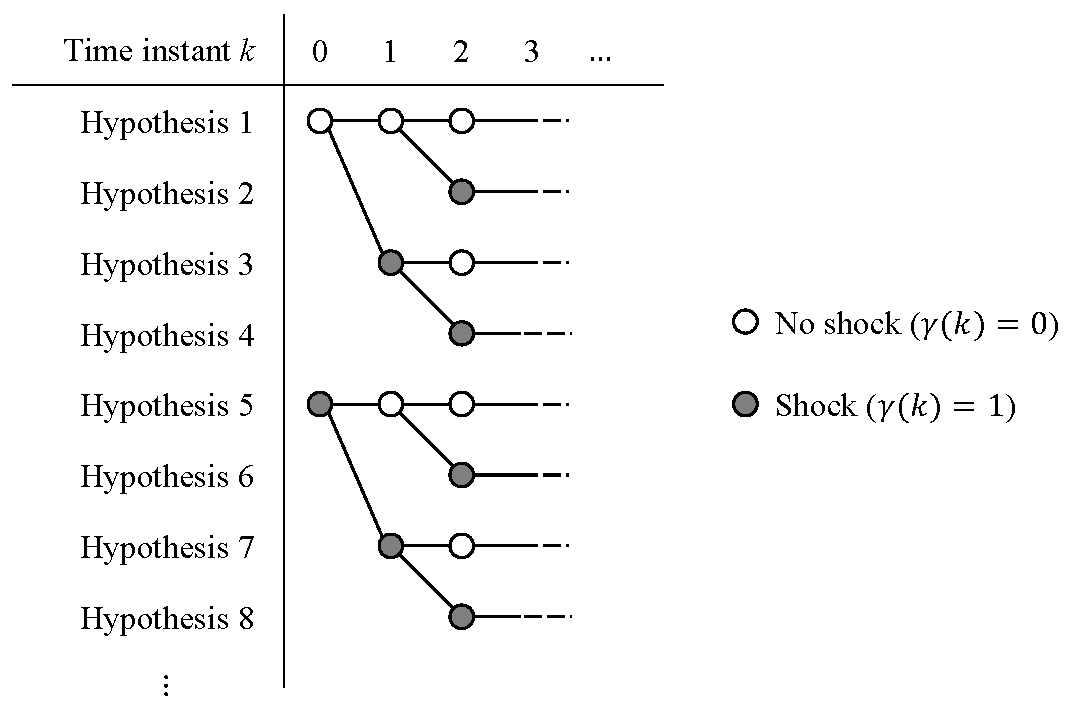
\includegraphics[height=7.5cm]{images/mm_obs_seq_br.pdf}
	\caption{Sequence branching}
	\label{fig:mm-obs-br}
\end{figure}

\subsubsection{Generalised pseudo-Bayes algorithm} \label{sec:GPB}

One of the simplest sub-optimal multiple-model methods is the \textit{generalised pseudo-Bayesian algorithm} \citep{buxbaum_recursive_1969, jaffer_estimation_1971, tugnait_detection_1982}. Although not used directly in this work, the method is described here because it is a starting point for understanding hypotheses branching and merging, which are techniques used in the sequence fusion algorithm described by \cite{robertson_detection_1995}.

There are two basic versions of the algorithm, the \acrlong{GPB1} (\acrshort{GPB1}), and the \acrlong{GPB2} (\acrshort{GPB2}). Figure \ref{fig:mm-obs-gpb1} shows a simplified diagram of the \gls{GPB1} process in the case of a system with two modes ($n_j=2$). A single estimate of the system states and error covariance at time $k$ is branched into $n_j$ hypotheses representing the possible modes of the system at that time. In this context, \textit{branching} simply means duplicating or cloning the hypothesis state estimates and error covariance into $n_j$ copies. These are then used to initialise $n_j$ Kalman filters. Each Kalman filter then makes a prediction of the states in the next time instant using the system model associated with one of the possible modes. In the next time instant, the $n_j$ predictions are corrected using the measurements, and the updated estimates are merged into a single set of estimates using the multiple-model observer merging procedure defined by (\ref{eq:xkyk_hat_MKF}, \ref{eq:Pk_MKF}). These branching and merging steps are then repeated at each subsequent time step.
\begin{figure}[ht]
	\centering
	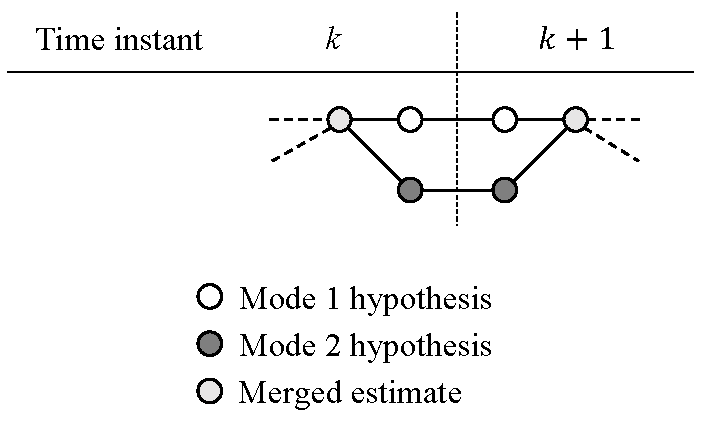
\includegraphics[height=5cm]{images/mm_obs_seq_gpb1.pdf}
	\caption{Simplified diagram of the \gls{GPB1} algorithm ($n_j=2$)}
	\label{fig:mm-obs-gpb1}
\end{figure}

Whereas the \gls{GPB1} estimator considers $n_j$ possible mode transitions from time $k-1$ to time $k$, the \gls{GPB2} estimator considers $n_j^2$ possible transition sequences from time $k-2$ to time $k$. Figure \ref{fig:mm-obs-gpb2} shows a simplified diagram of the \gls{GPB2} algorithm in the case of two system modes ($n_j=2$). At time $k$ it maintains $n_j$ merged estimates and associated variables, $\left\{ \hat{\mathbf{x}}_m(k \mid k), \mathbf{P}_m(k \mid k), \hat{\mathbf{y}}_m(k \mid k), \Pr(\Gamma_m(k) \mid \mathbf{Y}_M(k)) \right\}$, for $m=1,2,...,n_j$. Each of these is then branched into $n_j$ estimates, creating a total of $n_h=n_j^2$ hypotheses, represented by $n_h$ Kalman filters labelled $f=1,2,...n_h$. At time $k+1$, the Kalman filter predictions are corrected to produce $n_h$ estimates. Then, two merging operations are carried out on these estimates. The first merges the $n_h$ estimates into $n_m=n_j$ estimates for use in the next step. The second merges the $n_m$ merged estimates again, into one final estimate which is the output of the observer and is not used in subsequent steps.
\begin{figure}[ht]
	\centering
	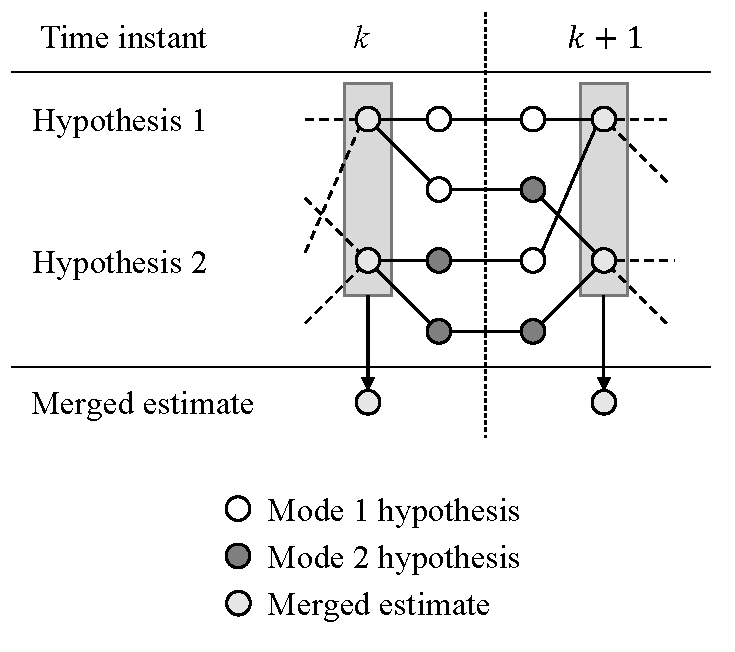
\includegraphics[height=6.5cm]{images/gpb2_diagram.pdf}
	\caption{Simplified diagram of the \gls{GPB2} algorithm ($n_j=2$)}
	\label{fig:mm-obs-gpb2}
\end{figure}

The $n_m$ merged estimates and covariances at time $k$ are produced by calculating weighted sums of the estimates and covariances of the branched hypotheses,
\nomenclature{$n_m$}{number of merged hypotheses maintained by a multiple-model observer}%
\nomenclature{$\mathbf{\hat{x}}_m(k \mid k)$}{merged estimates of the system states at time $k$ for merged hypothesis $m$}%
\nomenclature{$\mathbf{\hat{y}}_m(k \mid k)$}{merged estimates of the system outputs at time $k$ for merged hypothesis $m$}%
\nomenclature{$\mathbf{P}_m(k \mid k)$}{merged state estimation error covariance at time $k$ for merged hypothesis $m$}%
\nomenclature{$\Gamma_m(k)$}{merged shock hypothesis $m$ at time $k$}%
\begin{equation} \label{eq:xmkymk_hat_MKF}
	\begin{aligned}
		\mathbf{\hat{x}}_m(k \mid k) = \frac{1}{Z_m(k)} \sum_{f \in \mathcal{H}_{\text{merge},m}} \mathbf{\hat{x}}_f(k \mid k) \Pr(\Gamma_f(k) \mid \mathbf{Y}_M(k)), \\
		\mathbf{\hat{y}}_m(k \mid k) = \frac{1}{Z_m(k)} \sum_{f \in \mathcal{H}_{\text{merge},m}} \mathbf{\hat{y}}_f(k \mid k) \Pr(\Gamma_f(k) \mid \mathbf{Y}_M(k)),\\
		\mathbf{P}_m(k \mid k) = \frac{1}{Z_m(k)} \sum_{f \in \mathcal{H}_{\text{merge},m}} \Pr(\Gamma_f(k) \mid \mathbf{Y}_M(k)) \left( \mathbf{P}_f(k \mid k) + \delta_\mathbf{\hat{x}}(k) \delta_\mathbf{\hat{x}}^\intercal(k) \right), \\
		\delta_\mathbf{\hat{x}}(k) = \mathbf{\hat{x}}_m(k \mid k) - \mathbf{\hat{x}}_f(k \mid k), \\
		\Pr(\Gamma_m(k) \mid \mathbf{Y}_M(k)) = \sum_{f \in \mathcal{H}_{\text{merge},m}} \Pr(\Gamma_f(k) \mid \mathbf{Y}_M(k)).
	\end{aligned}
\end{equation}
\nomenclature{$\mathcal{H}_{\text{merge}}$}{hypothesis index used in merging operations}%
where $\mathcal{H}_{\text{merge}}$ is a set of $n_m$ indices that determine which hypotheses are merged to produce each merged estimate, and $Z_m(k)$ is a scalar normalization variable given by
\nomenclature{$Z_m(k)$}{normalization variable at time $k$ used in merged probability calculations}%
\begin{equation} \label{eq:Zmk}
	Z_m(k) = \sum_{f \in \mathcal{H}_{\text{merge},m}} \Pr(\Gamma_f(k) \mid \mathbf{Y}_M(k)).
\end{equation}

In the case of \gls{GPB2}, $\mathcal{H}_{\text{merge}}$ is defined
\begin{equation} \label{eq:Hmerge_GPB2}
	\mathcal{H}_{\text{merge}} = \begin{Bmatrix} \mathcal{H}_{\text{merge},1} \\ \mathcal{H}_{\text{merge},2} \end{Bmatrix} = \begin{Bmatrix}
		\begin{bmatrix}	1 \\ 3 \end{bmatrix} \\
		\begin{bmatrix}	2 \\ 4 \end{bmatrix}
	\end{Bmatrix}.
\end{equation}
This means that merged estimate $\mathbf{\hat{x}}_1(k \mid k)$ is calculated by merging the estimates associated with branched hypotheses 1 and 3, and merged estimate $\mathbf{\hat{x}}_2(k \mid k)$ is calculated by merging the estimates of branched hypotheses 2 and 4.

An associated index, $\mathcal{H}_{\text{branch}}$, governs the branching operation, which for \gls{GPB2} is
\nomenclature{$\mathcal{H}_{\text{branch}}$}{hypothesis index used in branching operations}%
\begin{equation} \label{eq:Hbranch_GPB2}
	\mathcal{H}_{\text{branch}} = \begin{bmatrix} 1 \\ 1 \\ 2 \\ 2 \end{bmatrix}.
\end{equation}
This indicates that branched estimates 1 and 2 are clones of merged estimate $\mathbf{\hat{x}}_1(k \mid k)$ and branched estimates 3 and 4 are clones of merged estimate $\mathbf{\hat{x}}_2(k \mid k)$. These definitions match the branching and merging operations depicted in Figure \ref{fig:mm-obs-gpb2}.

% TODO: We don't need this if we define the r(k) and r_m(k) transitions.
The system modes, which determine the system model parameters as well as the mode transition probabilities, evolve according to the branching and merging indices. Starting with the modes associated with the merged hypotheses at time $k$, which in the case of GPB2 are
\nomenclature{$\mathbf{r}_m(k)$}{indicators of the system modes of the merged hypotheses at time $k$ used in branching and merging operations}%
\begin{equation} \label{eq:rmk_GPB2}
		\mathbf{r}_m(k) = \begin{bmatrix} 1 \\ 2 \end{bmatrix},
\end{equation}
the branched modes after branching at time $k$ and before merging at time $k+1$ are
\nomenclature{$\mathbf{r}_{b,1}(k)$}{indicators of the system modes of the branched hypotheses at time $k$ before merging}%
\nomenclature{$\mathbf{r}_{b,2}(k)$}{indicators of the system modes of the branched hypotheses at time $k$ after branching}%
\begin{equation} \label{eq:rbk_GPB2}
	\begin{aligned}
		\mathbf{r}_{b,2}(k) &= \begin{bmatrix} 1 \\ 1 \\ 2 \\ 2 \end{bmatrix},
		\mathbf{r}_{b,1}(k+1) &= \begin{bmatrix} 1 \\ 2 \\ 1 \\ 2 \end{bmatrix}.
	\end{aligned}
\end{equation}
Note that $\mathbf{r}_{b,2}(k)$ is derived by branching $\mathbf{r}_m(k)$ using $\mathcal{H}_{\text{branch}}$ and that when $\mathbf{r}_{b,1}(k+1)$ is merged using $\mathcal{H}_{\text{merge}}$ in the next time step, it leads to 
\begin{equation} \label{eq:rmkp1rmk_GPB2}
	\mathbf{r}_m(k+1) = \begin{bmatrix} 1 \\ 2 \end{bmatrix} = \mathbf{r}_m(k).
\end{equation}
Due to this condition, the algorithm is consistent when executed consecutively every time step.

The advantages of the \gls{GPB1} and \gls{GPB2} estimators are their simplicity, the fact that they can be applied to any switching system, and that the number of hypotheses ($n_j$ or $n_j^2$) is finite and constant, which limits computational requirements. The disadvantages include the fact that they model every possible transition over one or two time steps and merge these into a reduced set of estimates before the next iteration. 

While the branching, modes, and merging steps of the \gls{GPB1} and \gls{GPB2} algorithms are the same each time step, they may be time-varying in the case of the sub-optimal multiple-model algorithms considered in this work. The notation above is easily extended to more complex algorithms with arbitrary branching and merging steps by allowing $\mathcal{H}_{\text{branch}}$, $\mathcal{H}_{\text{merge}}$, $\mathbf{r}_{b,1}(k)$, and $\mathbf{r}_{b,2}(k)$ to be time-varying and by allowing an arbitrarily large number of branched and merged hypotheses, $n_h$ and $n_m$, to exist at each time instant.

\subsubsection{Sequence fusion} \label{sec:fusion}

\cite{robertson_detection_1995} proposed a sub-optimal approach that combines three approximation techniques specifically intended for \gls{RODD} state estimation. The first is referred to as \textit{sequence fusion}. This is based on the assumption that only recent differences in the hypothesis sequences are important for state estimation. Therefore, sequences that are identical over the previous $N_f$ sample times may be merged, where $N_f$ is known as the \textit{fusion horizon}.
\nomenclature{$N_f$}{sequence fusion parameter: length of fusion horizon in number of sampling intervals}%
%The same techniques used in the generalized pseudo-Bayes algorithm are used to perform the sequence branching and merging at each time step. The differences are that more than $n_j^2$ hypotheses are maintained and these are based on longer, pre-specified sequences of possible shocks.

Rather than allowing the number and length of the shock indicator hypothesis sequences, $\Gamma_f(k)$, to grow indefinitely, a fixed number of sequences of length $N_f$ sample periods are defined, each consisting of only the current and the previous $N_f-1$ values of \hl{$\gamma(k)$}
\nomenclature{$\Gamma_m(k-N_f+1,k)$}{merged shock hypotheses $m$ at time $k$ for the fusion horizon $N_f$}%
\begin{equation} \label{eq:Gamma_kmf_k}
	\Gamma_m(k-N_f+1,k) = \{\gamma_m(k-N_f+1), ...,  \gamma_m(k-1), \gamma_m(k)\}, m=1,2,..., n_m.
\end{equation}
These fixed-length sequences are used to merge similar hypotheses so that the total number, $n_m$, remains the same from one time instant to the next.

Secondly, they assume that the exact timing of random shocks is not important and define \textit{detection intervals} of more than one sample period during which it is assumed that only one shock may occur. This is based on the observation that when the correction gain of a Kalman filter increases due to the assumption of a shock occurrence ($\gamma_m(k)=1$), it tends to remain large for several sample periods. The probability of at least one random shock during a detection interval of length $d$ samples is therefore higher than the probability, $\varepsilon$, of a single shock in one sample period, and is given by
\nomenclature{$d$}{sequence fusion parameter: shock spacing or length of detection interval, in number of sampling intervals}
\nomenclature{$\varepsilon_d$}{sequence fusion parameter: probability of at least one shock within the detection interval}%
\begin{equation}  \label{eq:p_gamma_d}
	\varepsilon_d = 1 - (1 - \varepsilon)^{d}.
\end{equation}

The occurrence of one or more shocks within a detection interval is then represented by a single shock at the start of the detection interval and the probabilities of a shock at any other time are set to zero,
\begin{equation} \label{eq:Pr_gamma_nd}
	\begin{aligned}
		\Pr\left(\gamma_{f}(k)=0\right) = \begin{cases*}
			1 - \varepsilon_d & \text { for } $k = d, 2d, 3d, \ldots$ \\
			1 & \text { for } $k \ne d, 2d, 3d, \ldots$
		\end{cases*} \\
		\Pr\left(\gamma_{f}(k)=1\right) = \begin{cases*}
			\varepsilon_d & \text { for } $k = d, 2d, 3d, \ldots$ \\
			0 & \text { for } $k \ne d, 2d, 3d, \ldots$
		\end{cases*} \\
	\end{aligned}
\end{equation}

Thirdly, they rely on the fact that the random shocks occur infrequently and therefore the probability of more than $n_\text{max}$ shocks during the fusion horizon is low, where $n_\text{max}$ may be 1 or some other low number. This further reduces the number of possible hypotheses that must be modelled.
\nomenclature{$n_\text{max}$}{sequence fusion parameter: maximum number of shock occurrences within the fusion horizon}%

To illustrate the resulting shock hypothesis sequences, consider an example. Suppose there is one \gls{RODD} to estimate. A sequence fusion algorithm is used with a fusion horizon of $N_f=9$, a detection interval of $d=3$, and a maximum number of shocks over the fusion horizon of $n_\text{max}=1$. Figure \ref{fig:mm-obs-seq-SFex1} shows the four shock hypotheses that would be required in this case. Note that hypothesis 1 assumes no shocks at any time. Hypothesis 2 assumes shocks occur at times $k=0,9,18,...$. Hypothesis 3 assumes shocks occur at times $k=3,12,21,...$, and so on. After $N_f=9$ sample periods, the sequences repeat indefinitely.

\begin{figure}[ht]
	\centering
	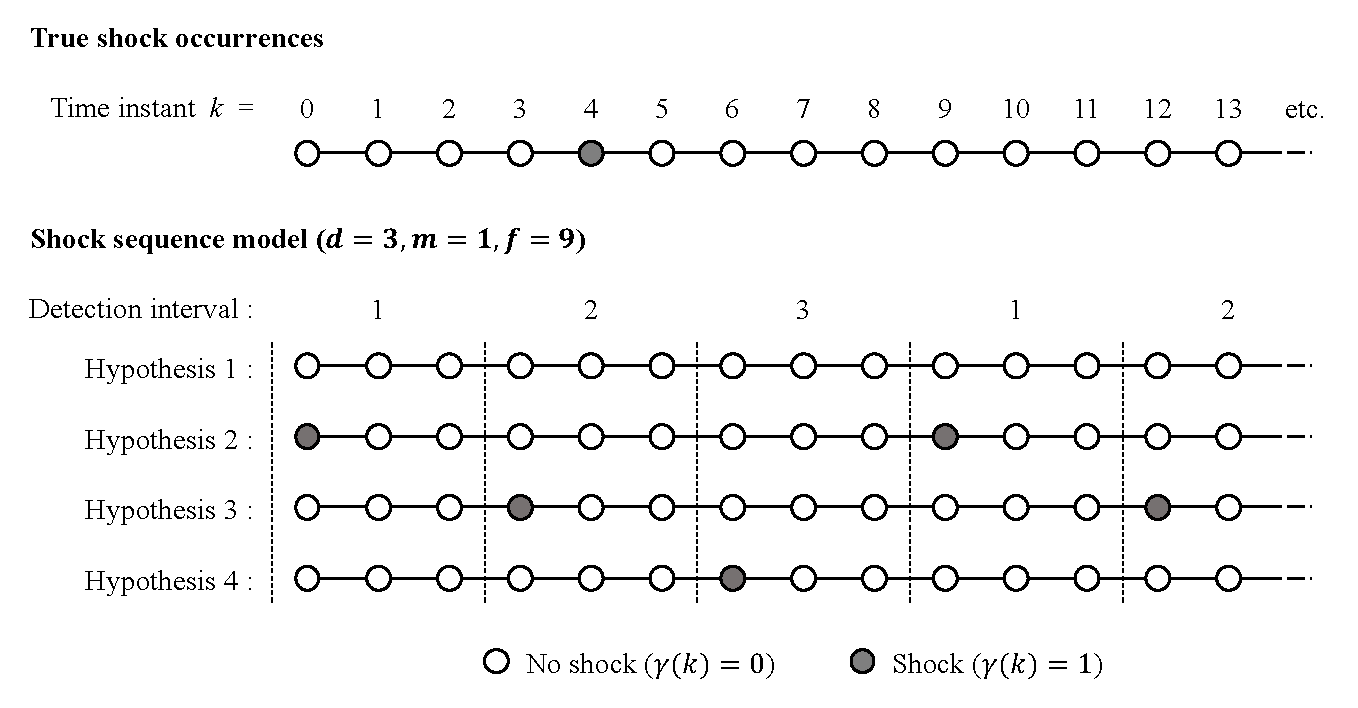
\includegraphics[width=13.5cm]{images/mm_obs_seq_rob1.pdf}
	\caption{Sequence fusion example 1 ($N_f=9$, $n_\text{max}=1$, $d=3$)}
	\label{fig:mm-obs-seq-SFex1}
\end{figure}

Suppose that a shock actually occurred in the system at time $k=4$. In this case, the algorithm should predict that hypothesis 3 is the most likely because this assumes a shock occurred at $k=3$, which is the closest to the actual time.

Figure \ref{fig:mm-obs-seq-SFex2} illustrates a second example with $N_f=10$, $n_\text{max}=2$, and $d=5$. This also has four hypotheses. However, note that hypothesis 4 accounts for the possibility of two shocks within the fusion horizon. As in the previous example, if a true shock occurred at time $k=4$, the most likely hypothesis should be hypothesis 3 because it assumes a shock occurred at $k=5$, which is close to the actual time.
\begin{figure}[ht]
	\centering
	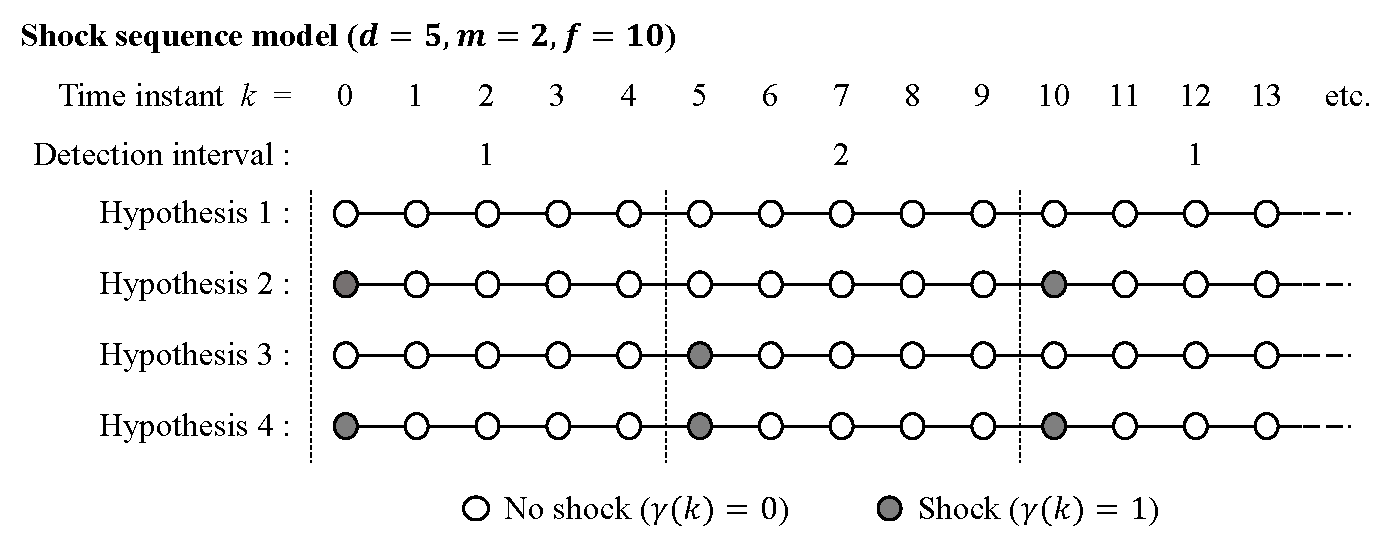
\includegraphics[width=13.5cm]{images/mm_obs_seq_rob2.pdf}
	\caption{Sequence fusion example 2 ($N_f=10$, $n_\text{max}=2$, $d=5$)}
	\label{fig:mm-obs-seq-SFex2}
\end{figure}

As mentioned, the shock hypothesis sequences over the fusion horizon, $\Gamma_m(k-N_f+1,k)$, determine the branching and merging operations that occur at each time step. The logic is as follows: (i) at time $k$, branch each hypothesis sequence into the possible mode transitions that occur between time $k$ and $k+1$, (ii) advance the branched sequences into the next time step, according to the possible mode transitions, (iii) compare the branched sequences and merge those that are identical over the new fusion horizon from time $k-N_f+2$ to $k+1$.

Consider again the sequences from the previous example in Figure \ref{fig:mm-obs-seq-SFex2}. By applying the logic described above, the branching and merging operations depicted in Figure \ref{fig:mm-obs-seq-sf95} may be deduced. For example, consider what happens at time $k=9$. At this time, the fusion horizon spans from time 0 to 9. The four sequences are branched into eight and advanced to the next time instant according to the possible modes at that time (no shock, shock). Then, at time $k=10$ the 8 branched hypotheses are merged back to 4 by combining sequences that are identical over the new fusion horizon, which spans from $k=1$ to 10. Applying this logic each time step, branching and merging are only required once every 5 time steps when shocks are assumed to be possible.
\begin{figure}[ht]
	\centering
	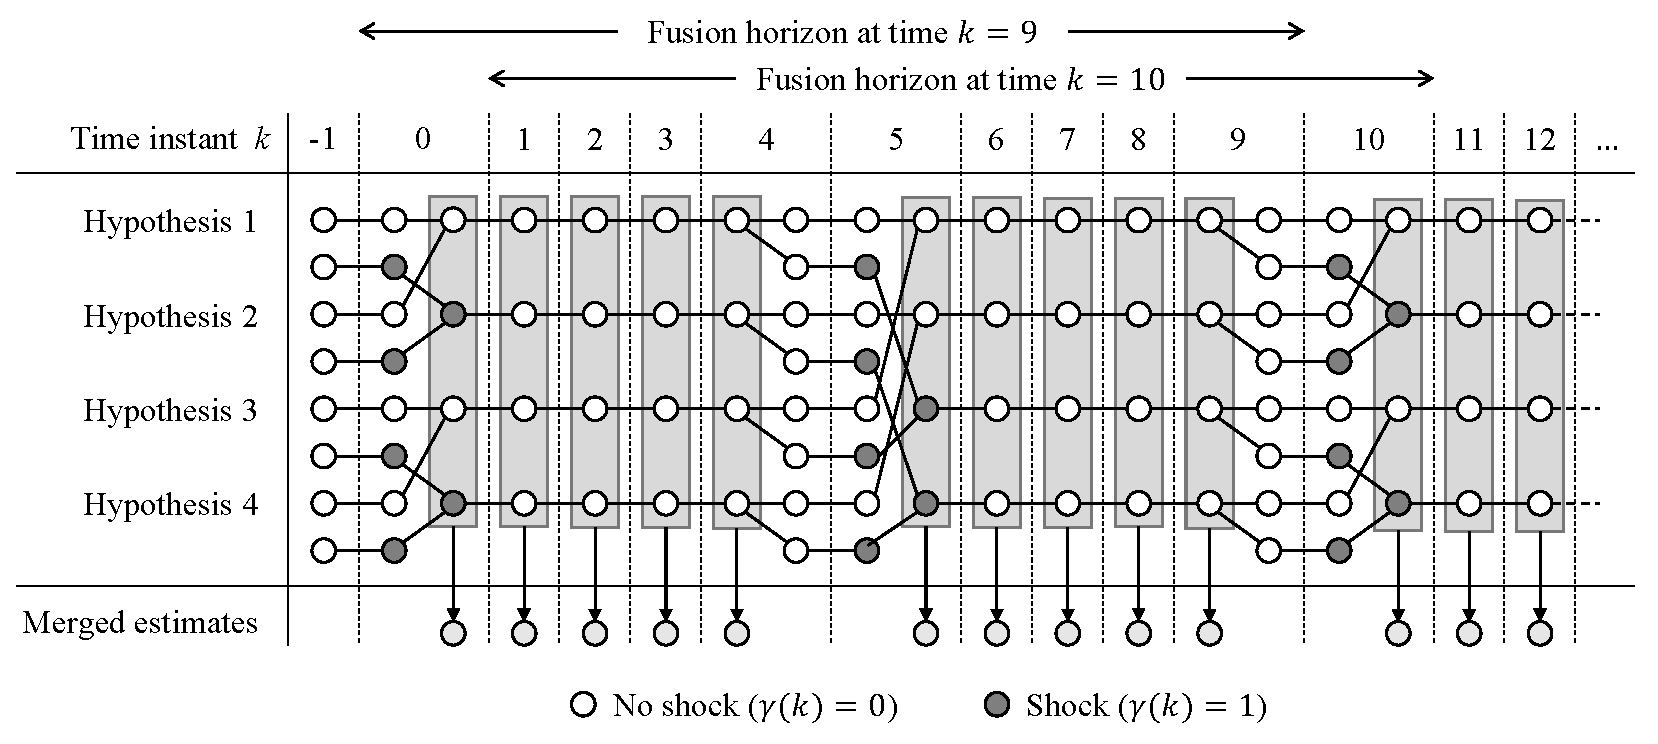
\includegraphics[width=15.5cm]{images/mm_obs_seq_sf95.pdf}
	\caption{Sequence branching and merging example ($N_f=10$, $n_\text{max}=2$, $d=5$)}
	\label{fig:mm-obs-seq-sf95}
\end{figure}

Rather than constant branching and merging indices, as in GPB2 (\ref{eq:Hbranch_GPB2}, \ref{eq:Hmerge_GPB2}), sequences of branching and merging indices are needed. In this example, they are
\begin{equation} \label{eq:Hbranch_SFex2}
	\mathcal{H}_{\text{branch}} = \begin{Bmatrix}
		\begin{bmatrix} 1 \\ 2 \\ 3 \\ 4 \end{bmatrix} &
		\begin{bmatrix} 1 \\ 2 \\ 3 \\ 4 \end{bmatrix} &
		\begin{bmatrix} 1 \\ 2 \\ 3 \\ 4 \end{bmatrix} &
		\begin{bmatrix} 1 \\ 2 \\ 3 \\ 4 \end{bmatrix} &
		\begin{bmatrix} 1 \\ 1 \\ 2 \\ 2 \\ 3 \\ 3 \\ 4 \\ 4 \end{bmatrix} &
		\begin{bmatrix} 1 \\ 2 \\ 3 \\ 4 \end{bmatrix} &
		\begin{bmatrix} 1 \\ 2 \\ 3 \\ 4 \end{bmatrix} &
		\begin{bmatrix} 1 \\ 2 \\ 3 \\ 4 \end{bmatrix} &
		\begin{bmatrix} 1 \\ 2 \\ 3 \\ 4 \end{bmatrix} &
		\begin{bmatrix} 1 \\ 1 \\ 2 \\ 2 \\ 3 \\ 3 \\ 4 \\ 4 \end{bmatrix}
	\end{Bmatrix},
\end{equation}
and
\begin{equation} \label{eq:Hmerge_SFex2}
	\mathcal{H}_{\text{merge}} = \begin{Bmatrix}
		\begin{bmatrix}	1 \\ 3 \end{bmatrix} & 1 & 1 & 1 & 1 & \begin{bmatrix}	1 \\ 5 \end{bmatrix} & 1 & 1 & 1 & 1 \\
		\begin{bmatrix}	2 \\ 4 \end{bmatrix} & 2 & 2 & 2 & 2 & \begin{bmatrix}	3 \\ 7 \end{bmatrix} & 2 & 2 & 2 & 2 \\
		\begin{bmatrix}	5 \\ 7 \end{bmatrix} & 3 & 3 & 3 & 3 & \begin{bmatrix}	2 \\ 6 \end{bmatrix} & 3 & 3 & 3 & 3 \\
		\begin{bmatrix}	6 \\ 8 \end{bmatrix} & 4 & 4 & 4 & 4 & \begin{bmatrix}	4 \\ 8 \end{bmatrix} & 4 & 4 & 4 & 4 \\
	\end{Bmatrix}.
\end{equation}

% Remove these: they don't add anything since these can be derived from the sequence
% and the branching/merging indices. Also, this convention for \Gamma_b and \Gamma_m
% was not defined. \Gamma_f was defined as single sequence and arguably would be
% better restricted to the merged sequences, than the branched ones.
%Likewise, the merged and branched shock (mode) indicator sequences are
%\begin{multline} \label{eq:Gamma_km09}
%	\glsadd{Gammafkmnk}\Gamma_m(0,9) = \left\{
%		\mathbf{\gamma}_m(0), \mathbf{\gamma}_m(1), \cdots, \mathbf{\gamma}_m(9)
%	\right\} = \\ 
%	\left\{
%		\begin{bmatrix} 0 \\ 1 \\ 0 \\ 1 \end{bmatrix},
%		\begin{bmatrix} 0 \\ 0 \\ 0 \\ 0 \end{bmatrix},
%		\begin{bmatrix} 0 \\ 0 \\ 0 \\ 0 \end{bmatrix},
%		\begin{bmatrix} 0 \\ 0 \\ 0 \\ 0 \end{bmatrix},
%		\begin{bmatrix} 0 \\ 0 \\ 0 \\ 0 \end{bmatrix},
%		\begin{bmatrix} 0 \\ 0 \\ 1 \\ 1 \end{bmatrix},
%		\begin{bmatrix} 0 \\ 0 \\ 0 \\ 0 \end{bmatrix},
%		\begin{bmatrix} 0 \\ 0 \\ 0 \\ 0 \end{bmatrix},
%		\begin{bmatrix} 0 \\ 0 \\ 0 \\ 0 \end{bmatrix},
%		\begin{bmatrix} 0 \\ 0 \\ 0 \\ 0 \end{bmatrix}
%	\right\}.
%\end{multline}
%\begin{multline} \label{eq:Gamma_kb09}
%		\Gamma_b(0,9 \mid 9) = \left\{\mathbf{\gamma}_b(0 \mid 0), \mathbf{\gamma}_b(1 \mid 1), \cdots, \mathbf{\gamma}_b(9 \mid 9) \right\} = \\
%		\left\{
%			\begin{bmatrix} 0 \\ 0 \\ 0 \\ 0 \end{bmatrix},
%			\begin{bmatrix} 0 \\ 0 \\ 0 \\ 0 \end{bmatrix},
%			\begin{bmatrix} 0 \\ 0 \\ 0 \\ 0 \end{bmatrix},
%			\begin{bmatrix} 0 \\ 0 \\ 0 \\ 0 \end{bmatrix},
%			\begin{bmatrix} 0 \\ 0 \\ 0 \\ 0 \\ 1 \\ 1 \\ 1 \\ 1 \end{bmatrix},
%			\begin{bmatrix} 0 \\ 0 \\ 0 \\ 0 \end{bmatrix},
%			\begin{bmatrix} 0 \\ 0 \\ 0 \\ 0 \end{bmatrix},
%			\begin{bmatrix} 0 \\ 0 \\ 0 \\ 0 \end{bmatrix},
%			\begin{bmatrix} 0 \\ 0 \\ 0 \\ 0 \end{bmatrix}
%			\begin{bmatrix} 0 \\ 0 \\ 1 \\ 1 \\ 0 \\ 0 \\ 1 \\ 1 \end{bmatrix},
%		\right\},
%\end{multline}
%\begin{multline} \label{eq:Gamma_kb110}
%		\Gamma_b(1,10 \mid 9) = \left\{ \mathbf{\gamma}_b(1 \mid 0), \mathbf{\gamma}_b(2 \mid 1), \cdots, \mathbf{\gamma}_b(10 \mid 9) \right\} = \\
%		\left\{
%			\begin{bmatrix} 0 \\ 1 \\ 0 \\ 1 \\ 0 \\ 1 \\ 0 \\ 1 \end{bmatrix},
%			\begin{bmatrix} 0 \\ 0 \\ 0 \\ 0 \end{bmatrix},
%			\begin{bmatrix} 0 \\ 0 \\ 0 \\ 0 \end{bmatrix},
%			\begin{bmatrix} 0 \\ 0 \\ 0 \\ 0 \end{bmatrix},
%			\begin{bmatrix} 0 \\ 0 \\ 0 \\ 0 \end{bmatrix},
%			\begin{bmatrix} 0 \\ 1 \\ 0 \\ 1 \\ 0 \\ 1 \\ 0 \\ 1 \end{bmatrix},
%			\begin{bmatrix} 0 \\ 0 \\ 0 \\ 0 \end{bmatrix},
%			\begin{bmatrix} 0 \\ 0 \\ 0 \\ 0 \end{bmatrix},
%			\begin{bmatrix} 0 \\ 0 \\ 0 \\ 0 \end{bmatrix},
%			\begin{bmatrix} 0 \\ 0 \\ 0 \\ 0 \end{bmatrix}
%		\right\}.
%\end{multline}
Although the number of branched hypotheses is time-varying, after $N_f$ time steps the sequences repeat such that
\nomenclature{$\mathbf{\gamma}_m(k)$}{vector of random shock indicators, $\gamma_f(k)$ for $f=1,2,...,m$, at time $k$}%
\begin{equation} \label{eq:rmkrmkmNf_SFex2}
	\mathbf{\gamma}_m(k) = \mathbf{\gamma}_m(k-N_f).
\end{equation}

As in the \gls{GPB2} algorithm, the overall estimates of the system states and outputs, $\hat{\mathbf{x}}(k \mid k)$ and $\hat{\mathbf{y}}(k \mid k)$, are calculated by merging the partially-merged estimates into one overall estimate. This is achieved by substituting $\mathbf{\hat{x}}_m(k \mid k)$ and $\mathbf{\hat{y}}_m(k \mid k)$ for $\mathbf{\hat{x}}_f(k \mid k)$ and $\mathbf{\hat{y}}_f(k \mid k)$ in \eqref{eq:xkyk_hat_MKF}.

\cite{robertson_detection_1995} described a systematic procedure to choose the parameters $N_f$, $n_\text{max}$, and $d$ and give the formula for the total probability of the modelled hypotheses as
\begin{equation} \label{eq:p_gamma}
	\beta=\operatorname{Pr}\left(\sum_{i=1}^{n} \gamma(i d) \leq n_\text{max} \right) = \sum_{j=0}^{n_\text{max}} \binom{n}{j} \varepsilon_d^{n-j}(1-\varepsilon_d)^{j},
\end{equation}
\nomenclature{$\beta$}{sequence fusion paramter: total probability of the modelled hypotheses, or in the case of the \acrshort{BRW}, a parameter of the additive bias function $a(\cdot)$}%
where $\binom{n}{j}$ represents the number of possible combinations of $j$ shocks in $n$ detection intervals. They recommended that the total probability should be at least 0.99 to ensure that only low-probability hypotheses are ignored.

In a later journal paper, \cite{robertson_method_1998} described a variation to the sequence fusion algorithm described above.  Rather than assuming that the shock occurs in the first sample period of each detection interval, as shown in Figures \ref{fig:mm-obs-seq-SFex1} and \ref{fig:mm-obs-seq-SFex2}, they proposed to represent the possibility of a shock as a sequence of $d$ smaller shocks such that the total variance over the detection interval is the same as that of one shock. They claimed this improved the performance of the algorithm in their simulations.

To implement this modification, define a new variable, $\delta(n)$, to represent whether or not at least one shock occurred during the $n$\textsuperscript{th} detection interval:
\nomenclature{$\delta(n)$}{sequence fusion variable: indicator of whether one or more shocks occurred in detection interval $n$}
\begin{equation} \label{eq:deltak}
	\delta(n) = \begin{cases*}
		0 & \text{if} $\sum_{k=(n-1) d}^{n d - 1}{\gamma(k)} = 0$, \\
		1 & \text{if} $\sum_{k=(n-1) d}^{n d - 1}{\gamma(k)} \ge 1$.
	\end{cases*}
\end{equation}

Then, replace the random shock variable used at each sample time, $w_p(k)$ \eqref{eq:wpk2}, with:
\begin{equation} \label{eq:wpdk}
	w_{p,d}(k) \sim 
	\begin{cases*}
		\mathcal{N}\left(0, \sigma_{w_p}^2\right) & \text{when} $\delta(n) = 0$, \\
		\mathcal{N}\left(0, \frac{b^2\sigma_{w_p}^2}{d}\right) & \text{when} $\delta(n) = 1$.
	\end{cases*}
\end{equation}

Note that the variance of a single shock, $b^2\sigma_{w_p}^2$, has ben divided by the detection interval length $d$. In this version of the algorithm, the branching and merging operations are only carried out at the end of each detection interval. In the steps within the detection interval, the Kalman filters are updated using the measurements, but no branching or merging occurs.

Figure \ref{fig:mm-obs-seq-sf98} shows the shock hypothesis sequences and the merging and branching steps of the 1998 version of the sequence fusion algorithm with the same parameters as in the previous example.
\begin{figure}[ht]
	\centering
	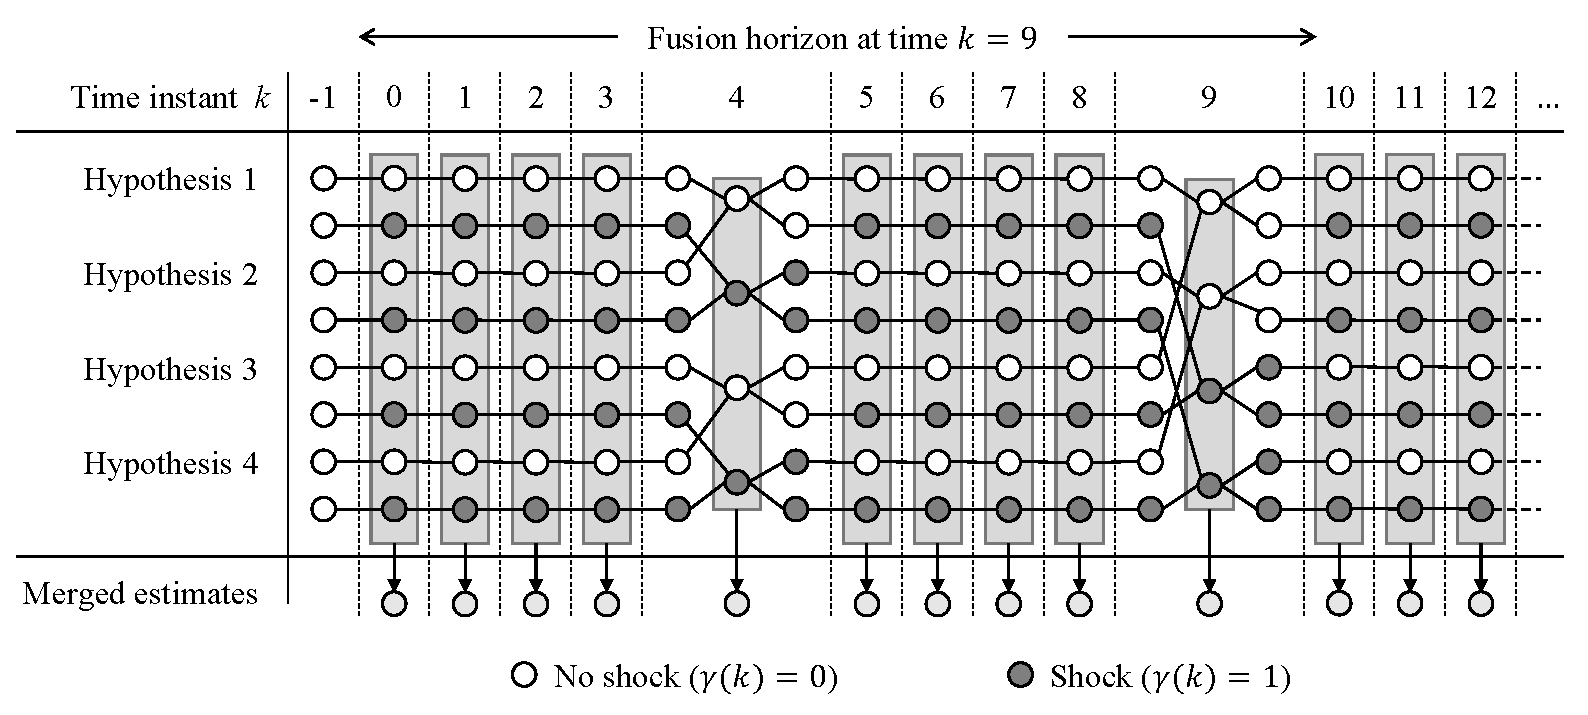
\includegraphics[width=15cm]{images/mm_obs_seq_sf98.pdf}
	\caption{Sequence branching and merging example – 1998 version ($N_d=5$, $n_\text{max}=2$, $N_f=10$)}
	\label{fig:mm-obs-seq-sf98}
\end{figure}
Note the two main differences when compared to Figure \ref{fig:mm-obs-seq-sf95}. Firstly, the system mode indicators are the same throughout the detection interval, whereas in the 1995 version the shocks were assumed to occur only at the first sample time of each detection interval. Secondly, after branching, the $n_h$ hypotheses are maintained for the duration of the detection interval before being merged and branched at the last sample time of the detection interval. The idea of these modifications is to allow $N_d$ Kalman filter updates to occur with the adjusted shock probability and variance (\ref{eq:p_gamma_d}, \ref{eq:wpdk}) before evaluating and merging the estimates. This was expected to produce better estimates of the hypothesis probabilities in situations where it takes more than one time step to detect changes in the system.

\subsubsection{Sequence pruning} \label{sec:pruning}

\textit{Sequence pruning} is the selective deletion of shock hypotheses that have a low likelihood given the current measurements. \cite{eriksson_classification_1996} used the \textit{adaptive forgetting through multiple models} (\acrshort{AFMM}) algorithm by \cite{andersson_adaptive_1985} for \gls{RODD} estimation. The \gls{AFMM} uses sequence pruning to limit the number of hypotheses and filters. The current hypotheses at each time instant are ranked according to their conditional probabilities \eqref{eq:Pr_Gammak_given_Yk}. The hypothesis with the lowest probability is then pruned with the caveat explained below. The most probable hypothesis is allowed to branch but all other hypotheses are advanced assuming no shock occurs in the next time period (i.e. all but one of their branches are pruned). This makes sense in the case of \gls{RODD} disturbances because the probability of a shock is low. Thus, the total number of hypotheses and filters is capped at a fixed number, $n_h$.

The caveat mentioned above, is that no hypothesis may be eliminated less than $N_\text{min}$ time steps after being created. This is to prevent good hypotheses from being eliminated before the conditional probabilities have been properly estimated, which can take more than one sample period. For this reason, $n_h$ must be at least sufficient to accommodate the \textit{minimum life}, $N_\text{min}$, of all new hypotheses. Note that in the case of systems with more than one \gls{RODD} disturbance, the number of branches of the most likely sequence is more than two, \hl{and the same number} of sequences will be pruned at each sample time.
\nomenclature{$N_\text{min}$}{sequence pruning parameter: minimum life of a branched hypothesis in number of sampling intervals}%

To illustrate the sequence pruning procedure, consider the diagram in Figure \ref{fig:mm-obs-seq-SP}. This shows one possible evolution of the hypothesis sequences in response to an actual shock sequence consisting of one shock at time $k=4$.  The most likely hypotheses at each time instant, identified by the circles with thicker outlines, branch into two at the next time instant. After the limit of five hypotheses is reached, one hypothesis is pruned at each sample time and replaced by a new branched hypothesis at the next. Note that at time $k=6$, hypothesis 2 becomes the most likely based on the available measurements at that time. Also note that no new branches are terminated in less than two sample times.
\begin{figure}[ht]
	\centering
	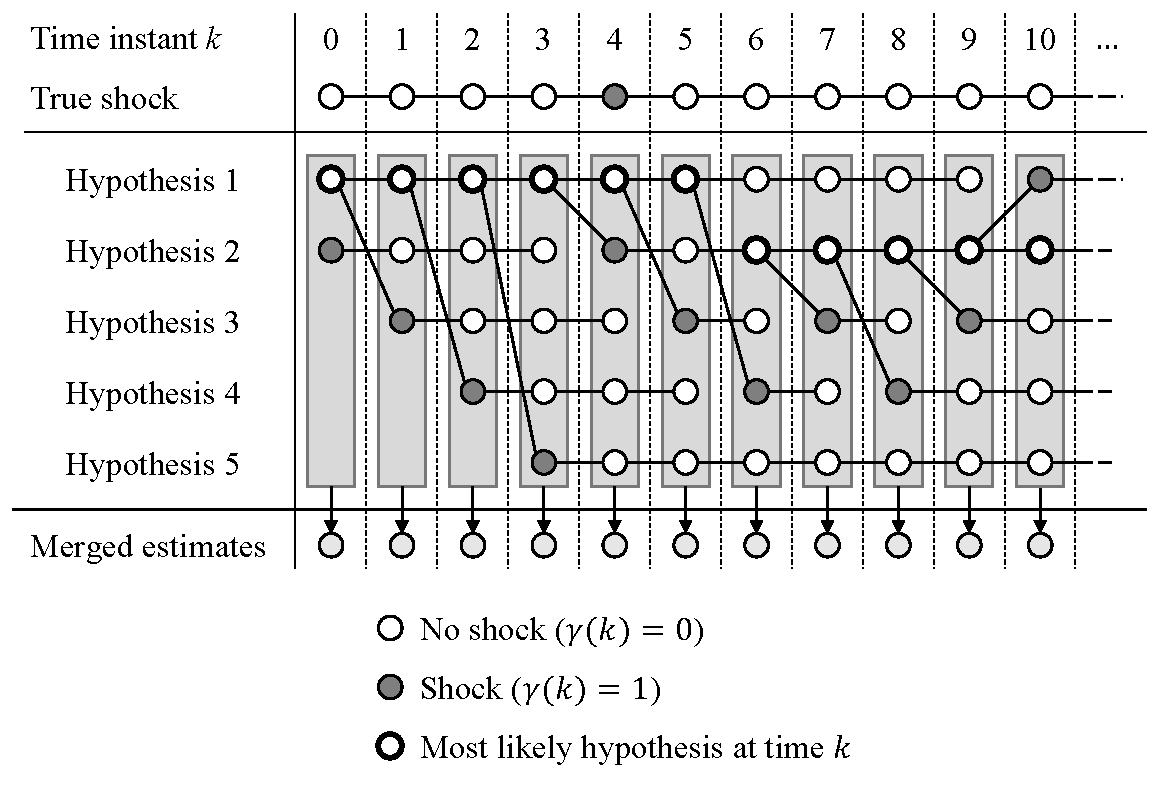
\includegraphics[width=10.7cm]{images/mm_obs_seq_SP.pdf}
	\caption{Sequence pruning example ($n_h=5$, $N_\text{min}=2$)}
	\label{fig:mm-obs-seq-SP}
\end{figure}

The \gls{AFMM} algorithm includes a complementary procedure for online estimation of the measurement noise covariance, $\mathrm{R}(k)$. This component was not implemented in this work since it is assumed that the variance of the measurement noise is time-invariant.

\subsubsection{Implementation details} \label{sec:implementation}

The diagram in Figure \ref{fig:mkf-infoflow} depicts the general computation steps and information flows of the sub-optimal multiple-model observers, as implemented in this work. The solid black rectangles represent computation steps and the \hl{coloured lines} represent the main variables. Steps 1 and 2 are the prediction steps of the Kalman filters (\ref{eq:xfkp1_hat}, \ref{eq:yfk_pred}), step 3 is the calculation of the prior probabilities of the hypotheses \eqref{eq:Pr_Gammak_given_Ykm1}, step 4 is the hypotheses evaluation step (\ref{eq:Pr_Gammak_given_Yk}, \ref{eq:qfk}), and step 5 is the Kalman filter update step (\ref{eq:xfkyfk_hat}, \ref{eq:Pkf-stab}). Step 6 is a place-holder for the sub-optimal procedures which depend on the specific algorithm but in this work include some combination of sequence branching, pruning, and merging. During this step, the final estimates of the states and outputs are also calculated.

\begin{figure}[ht]
	\centering
	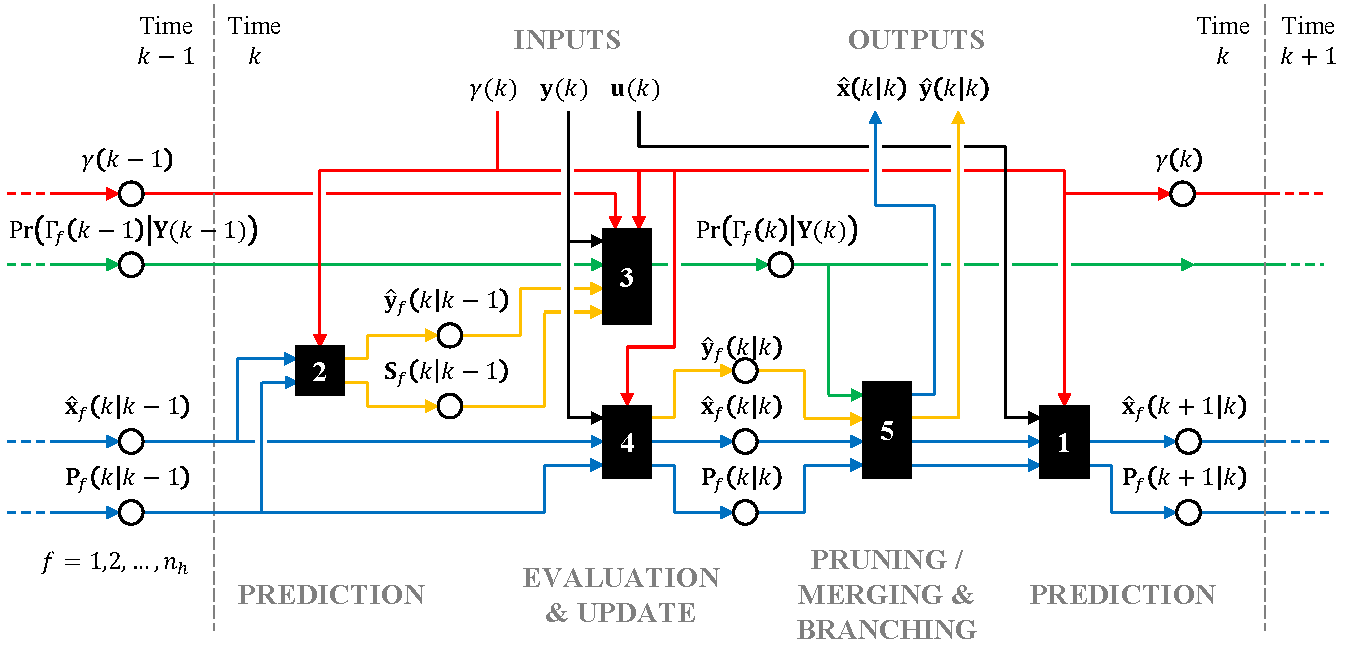
\includegraphics[width=15.5cm]{images/mkf_infoflow.pdf}
	\caption{General information flow diagram of a multiple-model observer}
	\label{fig:mkf-infoflow}
\end{figure}

At time $k$, the algorithm requires a mode indicator vector, $\gamma(k)=\begin{bsmallmatrix} \gamma_1(k) & \cdots & \gamma_{n_h}(k) \end{bsmallmatrix}^\intercal$, the system output measurement, $\mathbf{y}_M(k)$, and input, $\mathbf{u}(k)$, and produces estimates of the states, $\hat{\mathbf{x}}(k \mid k)$, and outputs, $\hat{\mathbf{y}}(k \mid k)$. The mode indicator vector is either constant, as in the case of the \gls{GPB1} and \gls{GPB2} algorithms or is specified by the sub-optimal procedure at each time step. At the end of each time step, the mode indicator vector, conditional hypothesis probabilities, one-step-ahead state predictions, and the prediction error covariances for each hypothesis are stored for use in the next time step. The sub-optimal algorithm, which determines $\gamma(k)$ as well as the merging, pruning, and branching procedures in step 6, may have other variables that need to be stored. These are not shown on the diagram. The total number of hypotheses modelled, $n_h$, also depends on the algorithm, and may be time-varying.

\section{System identification} \label{sec:sys-id}

% Some text not used in IFAC report
Model-based observers such as the Kalman filter require a dynamic model of the process. In practice, models of the process dynamics are not available but they can be identified when input-output data sampled from the process is available. In this case, system identification methods are common practice, as described by \cite{ljung_system_1999} among others.

To construct a multiple-model observer for systems with \gls{RODD}s, the structure and parameters of the disturbance model as well as the process model are needed. \gls{RODD}s are discrete-time \acrlong{MJLS} (\acrshort{MJLS}) \citep{costa_discrete-time_2005}. Standard approaches to system identification such as least-squares regression are not applicable to hybrid dynamical systems with both discrete and continuous states. Identification of these types of systems is challenging and the subject of \hl{recent} research. See for example, \cite{bemporad_fitting_2018} and \cite{piga_estimation_2020}.

%Outline notes:
%\begin{itemize}
%	\item Explain Isaksson and Eriksson's perspective on standard system identification approach.
%	\item Explain distinction between system detection or `discrimination' and system identification, reference Isaksson and Eriksson's paper on disturbance classification (whether disturbance at input or output of process).
%	\item Introduce other approaches—MLE, EM algorithm (Dempster et al., Wong \& Lee)
%	\item Methods proposed by Bemporad (Fitting jump models, 2018 and Jump Box-Jenkins, 2020).
%	\item Theory and challenges Costa book. Others?
%	\item In recent years, numerical methods to overcome the intractability of the probabilistic integral have received a lot of attention.
%	\item Sequential Monte-Carlo methods, (incl. particle filtering), Stochastic Variational Inference, ... (read Special issue in IEEE control magazine for an overview of these methods)
%\end{itemize}

% More text from IAFAC paper:
%are assumed to be known and were set to match the characteristics of the simulated disturbance. In practice, they would have to be estimated, either using prior knowledge of the disturbance source, or possibly from system output measurements using an appropriate system identification method---see \cite{schon_sequential_2015} for one possible approach---provided a sufficiently long sequence of data is available.

% Note: may remove this if we aren’t using any formal methods.

%\section{Control strategies}
%
%In this work, the goal is to test the performance of different observers in a closed-loop feedback control application (not to evaluate different control strategies). Therefore, only one control strategy is considered. According to the \textit{separation principle} of estimation and control, the control strategy may be designed independently of the observer. The controller is designed using the same augmented system model, including the plant model and disturbance models, that is used in the observer design. However, the switching behaviour of the random shock variable used in the \gls{RODD} is not explicitly considered in the control design. The estimates of the model states produced by the observer are assumed to be optimal, i.e. the expected values, and their uncertainty is not taken into account by the control algorithm or in its design.
%
%
%\subsection{Model predictive control}
%
%\textit{\acrlong{MPC}} (\acrshort{MPC}) is a well known and widely used multi-variable control algorithm used in industrial applications. This is largely due to the fact that constraints can be imposed on the manipulated variables and control variables, as well as its intuitive design and the ease with which it can be tuned to achieve control objectives \citep{maciejowski_predictive_2002}. Although it is a computationally complex algorithm, numerous proven commercial products exist to enable its implementation.
%
%\gls{MPC} utilizes a prediction equation based on the dynamic model of the system to find feasible future trajectories of the system outputs as a function of the manipulated variables and the states of the model at the current time. The length of the prediction horizon, \gls{Hp}, is defined in terms of the number sample times starting at the next time instant, $k+1$. The predicted outputs over the prediction horizon, calculated at the current time $k$, are denoted $\hat{\textbf{y}}(k+i | k)$ for $i=1,2,...,H_p$. The length of the control horizon, \gls{Hc}, is defined starting at the current time, $k$, and the manipulated inputs are denoted $\mathbf{u}(k+i-1)$ for $i=1,2,...,H_c$. The control horizon is usually shorter than the prediction horizon, in which case, $\mathbf{u}(k+j)=\mathbf{u}(k+H_c-1)$ for $j=H_c,H_c+1,...,H_p$.
%
%The constrained optimization problem, which is solved at each time step, is
%\begin{align} \label{eq:mpc-opt}
%	\begin{split}
%		\min _{\mathbf{u}(k), \mathbf{u}(k+1), \ldots, \mathbf{u} (k+H_c-1)}
%		& \quad \sum_{i=1}^{H_{p}}[\mathbf{\hat{y}}(k+i / k) - \mathbf{r}(k+i)]^\intercal \mathbf{\Phi} [\mathbf{\hat{y}}(k+i / k) - \mathbf{r}(k+i)] \\
%		& \qquad + \sum_{i=1}^{H_{c}}[\Delta \mathbf{u}(k+i-1)]^\intercal \mathbf{\Lambda} [\Delta \mathbf{u}(k+i-1)] \\
%			\end{split} \\
%		\text { subject to: }
%		&\ \mathbf{u}_{min} \leq \mathbf{u}(k+j-1) \leq \mathbf{u}_{max} \quad  j=1,2, \dots, H_{c} \label{eq:mpc-cons-1}, \\
%		& \Delta \mathbf{u}_{min} \leq \Delta \mathbf{u}(k+j-1) \leq \Delta \mathbf{u}_{max} \quad j=1,2, \dots, H_{c}, \label{eq:mpc-cons-2} \\
%		& \mathbf{y}_{min} \leq \mathbf{\hat{y}}(k+j / k) \leq \mathbf{y}_{max} \quad  j=1,2, \dots, H_{p}, \label{eq:mpc-cons-3}
%\end{align}\textbf{[TODO: Consider including slack variables to ensure feasibility]}
%where $\mathbf{r}(k+i)$ for $i=1,2,...,H_p$ is the reference output trajectory, and $\Delta \mathbf{u}(k)$ is the change in the manipulated variable at time $k$, defined as $\Delta \mathbf{u}(k) = \mathbf{u}(k) - \mathbf{u}(k-1)$. The tunable parameters are $H_p$, $H_c$, $\mathbf{\Phi}$, and $\mathbf{\Lambda}$, and the constraints are $\mathbf{u}_{min}$, $\mathbf{u}_{max}$, $\Delta \mathbf{u}_{min}$, $\Delta \mathbf{u}_{max}$, $\mathbf{y}_{min}$, and $\mathbf{y}_{max}$. Note that the last constraint \eqref{eq:mpc-cons-3} only guarantees that the estimate of the system output will not violate the constraints. This does not imply that the true system output will respect them at all times.
%
%Once a solution to the optimization problem is found, only the control actions at the current time, $\mathbf{u}(k)$, are transmitted to the plant. The procedure is then repeated every future time instant to compute the subsequent control actions. This is referred to as \textit{receding horizon control}.


\section{Grinding simulation model} \label{sec:grinding-simulator}

%Outline notes:
%\begin{outline}
%    \1 Assumptions and limitations: constant breakage rate model, relationships between speed, media, trajectories, filling level and breakage not captured.
%	\1 Describe grate, transport delays and cyclone model.
%	\1 Outline any significant changes made from Edgar's model
%	\1 Figure: simulation results showing steady-state characteristics - e.g. power, grind, and throughput vs. fill level and speed.
%	\1 Figure \ref{fig:coarse_fine_psd_plot}: Particle size distributions of feed, recirculating load and product - this should help explain steady-state characteristics.
%	\1 Figure - Step responses of main process variables to changes in ore properties.
%	\1 Selection of particle size distribution as the disturbance variable for this work.
%	\1 Steady-state characteristics with operating points (grind curves)\\
%\end{outline}

A dynamic simulation model of the primary grinding circuit of a gold mine in Quebec is used to simulate the effects of changes in ore feed properties on the grinding circuit over time. The model was developed by \cite{perez_garcia_dynamic_2020} following the methodology described by \cite{grimble_dynamic_2010} and was calibrated to match operating data collected from the plant \citep{perez-garcia_systematic_2020}. Grinding in the \acrshort{SAG} mill is simulated by a \textit{population balance model} with 24 discrete ore particle size intervals and constant specific-energy selection rates (i.e. breakage rates are proportional to total energy consumption) and a constant breakage matrix.

Figure \ref{fig:sag-diag} is a simplified diagram of the simulated \acrshort{SAG} mill, which is in a closed circuit consisting of a feed conveyor, pump box, pump, and a bank of hydro-cyclones.
\begin{figure}[ht]
	\centering
	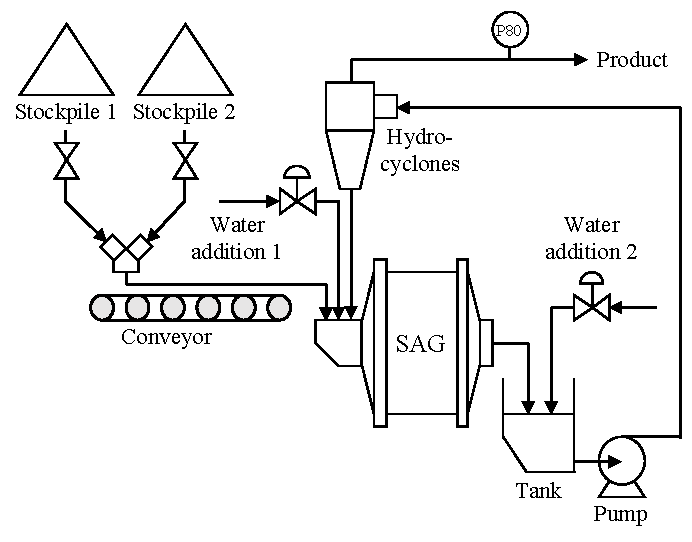
\includegraphics[width=12.5cm]{images/sag-circuit-diag.pdf}
	\caption{Simplified process flow diagram}
	\label{fig:sag-diag}
\end{figure}
For the purposes of this work, two ore feed streams with different \gls{PSD}s were simulated. Each stream is a different mix of two different ores. One ore has a fine \gls{PSD} and the other is coarse. The mix for stream \#1 (`mix 1') consists of 22.83\% coarse ore (\textit{mix factor} of 0.2283) and mix \#2 is an even mix of both ores (mix factor of 0.5). The two streams are mixed before discharging onto the conveyor. Figure \ref{fig:coarse_fine_psd_plot} shows the \gls{PSD}s of the two mixtures.
\begin{figure}[ht]
	\centering
	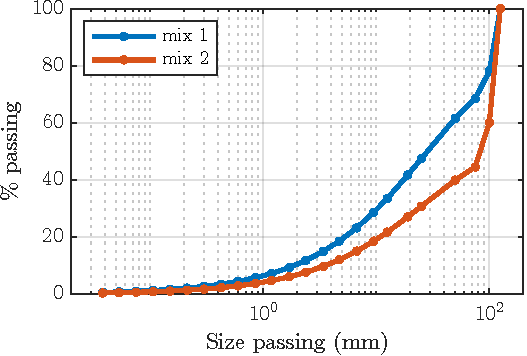
\includegraphics[width=9cm]{images/coarse_fine_cumpsd_plot.pdf}
	\caption{Ore particle size distributions}
	\label{fig:coarse_fine_psd_plot}
\end{figure}

The simulated instrumentation is also illustrated in Figure \ref{fig:sag-diag}. \hl{The setpoint of the water addition flowrate to the mill inlet (`water addition 1') is set to a fixed ratio of the ore feed rate.} The pump-box \hl{(`tank')} has a \gls{PI} controller to control the level to a fixed set-point by manipulating the water addition flow rate set-point (`water addition 2'). The main process variable used in this work is the product P80 measurement, which is a simulated online analyser that estimates the 80\% passing size of the material \hl{in the slurry} leaving the circuit. In this work, the inlet water addition ratio, the conveyor speed, the discharge pump speed, and the mill rotational speed are all fixed.

%The simulated instrumentation is also illustrated in Figure \ref{fig:sag-diag}. The \acrshort{SAG} mill water addition set-point is set by ratio control to a fraction of the fresh ore feed rate, which is measured on the conveyor. This water addition ratio is also manipulated. The pump-box level has a PI (proportional-integral) controller to control the level to a fixed set-point by manipulating the water addition flow rate set-point. The discharge pump speed is fixed. Conveyor speed is adjusted automatically in response to the fresh ore feed rate set-point. The \acrshort{SAG} rotational speed set-point may also be manipulated.
%
%The measurable process variables used in this work are the mill weight, which includes the weight of the shell and liners as well as the mill contents, mill power consumption, the solids-content of the cyclone feed stream, and the particle size (P80) of the ground product in the cyclone overflow. Mill filling level and other simulation variables are available for analysis but are assumed to be unmeasured in the real operation and therefore not available for process control.  Figure \ref{fig:grind_sim_io_diag} summarizes the inputs and outputs of the simulation model. Table \ref{tb:grind-vars} lists the normal operating points, units, and minimum and maximum operating limits of each variable.
%
%%TODO: Table of process variables and normal operating points, limits etc.
%\begin{table}[ht]
%	\centering
%	\caption{Grinding simulation model inputs and outputs} \label{tb:grind-vars}
%	% See: https://texblog.org/2019/06/03/control-the-width-of-table-columns-tabular-in-latex/
%	% Also: https://www.overleaf.com/learn/latex/Tables
%	\begin{tabular}{c c >{\raggedright}p{5.5cm} c c c c}
%		%\toprule
%		& Label & Description & Op. pt. & Units & Min. & Max \\
%		\midrule
%		\multicolumn{7}{l}{\textit{manipulated variables}} \\
%		%\midrule
%		  & MV1       & Ore feed rate & 122.7 & tons/h & 0 & 200 \\   
%		  & MV2       & Mill speed (fraction of critical speed) & 0.77 & - & 0 & 0.85 \\ 
%		  & MV3       & Water addition ratio (fraction of ore feed rate) & 0.341 & - & 0 & 1 \\ 
%		%\midrule
%		\multicolumn{7}{l}{\textit{Unmeasured disturbance input}} \\
%		%\midrule
%		  & UD1        & Ore mix factor & 0.2283 & - & 0 & 1  \\ 
%		%\midrule
%		\multicolumn{7}{l}{\textit{Output variables}} \\
%		%\midrule
%		  & OV1        & Mill weight & 279.4 & tons & 100 & 320  \\ 
%		  & OV2       & Mill power consumption & 2391 & kW & 0 & 2400  \\ 
%		  & OV3       & Cyclone feed solids fraction & 61.4 & \% & 50 & 70  \\ 
%		  & OV4       & Cyclone overflow P80 & 105.4 & \% & 0 & 200  \\ 
%		\bottomrule
%	\end{tabular}
%\end{table}

%To better understand the relationships between the input and output variables, a set of simulations were carried out to determine steady-state operating conditions in the vicinity of the normal operating point. Figure \ref{fig:grind_sim_ss_plot1} shows how the steady-state values of the four output variables are affected by changes in the mill fill level (fraction of internal volume occupied by the charge) and rotation speed. The normal operating points are also shown, represented by solid markers. For these simulations, a simple PI controller was used to control the mill filling level by manipulating the ore feed rate and each simulation was run until all variables converged to steady-state values. However, no constraints were imposed during these simulations, therefore power consumption exceeds the maximum possible in some cases.
%
%These results are equivalent to the grind curves proposed by \cite{powell_applying_2009} for evaluating steady-state characteristics and optimal operating points for \acrshort{SAG} mills. However, compared to the curves presented by \cite{powell_applying_2009}, which were based on measurements from real operations, these are noticeably much closer to straight lines (i.e. linear relationships).
%
%A similar set of simulations were carried out to understand the effect of changing the ore mix factor on the steady-state values of the output variables. The results are shown in Figure \ref{fig:grind_sim_ss_plot2}. From these it can be seen that the change in ore mix has no effect on the steady-state power consumption of the mill. However, there are changes in the steady-state throughput (ore feed rate), cyclone feed solids fraction, and product particle size. The throughput is approximately 4 tons-per-hour higher and the product particle size is 1.5 microns smaller when the ore mix contains the higher fraction (0.5) of coarse ore.
%
%\begin{figure}[ht]
%	\centering
%	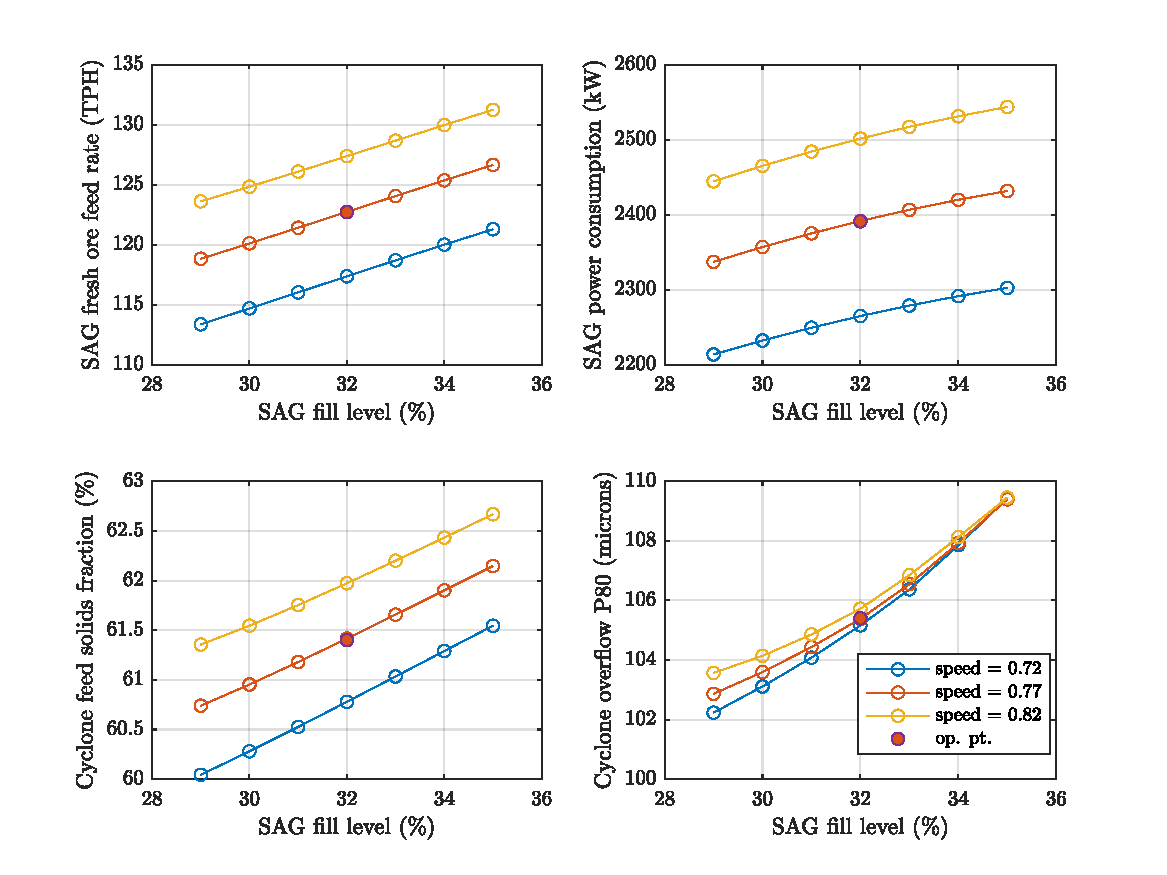
\includegraphics[width=15cm]{images/grind_sim_ss_plot1.pdf}
%	\caption{Steady-state operating points}
%	\label{fig:grind_sim_ss_plot1}
%\end{figure}
%
%\begin{figure}[ht]
%	\centering
%	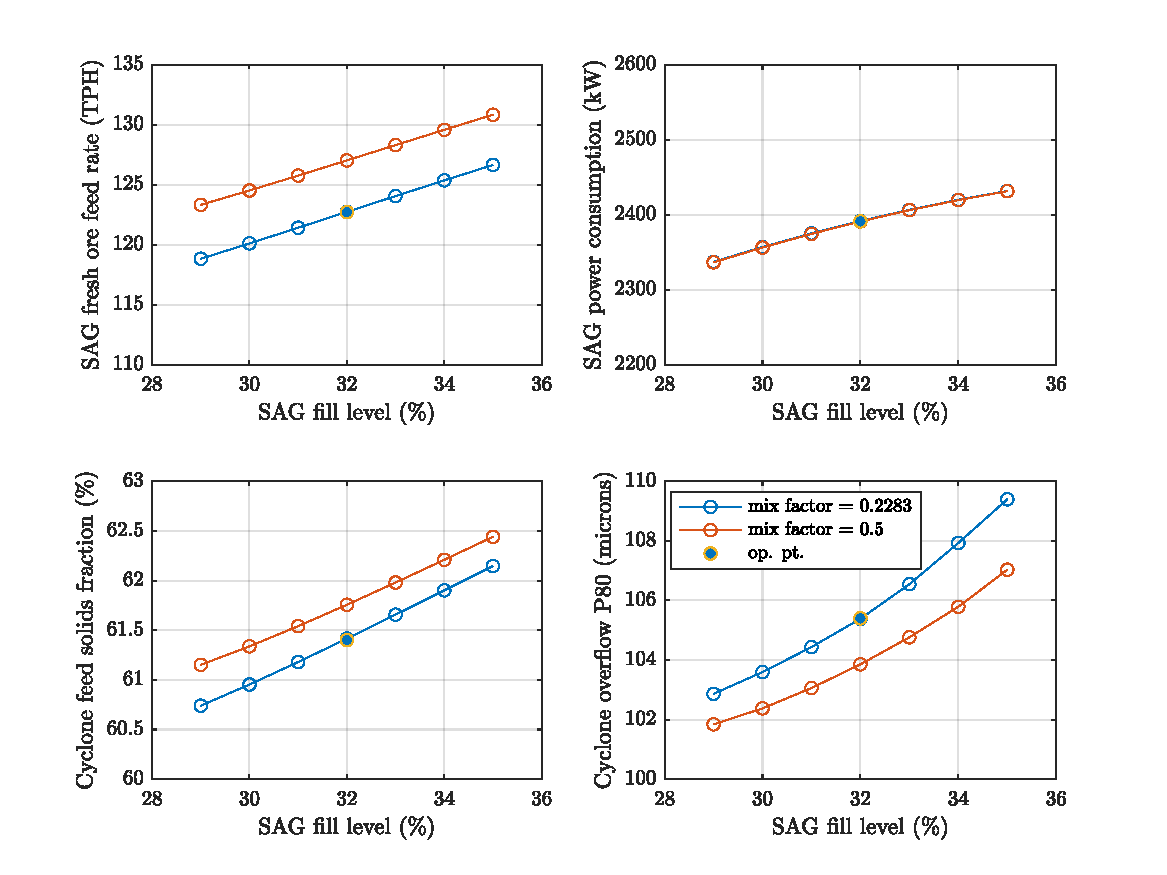
\includegraphics[width=15cm]{images/grind_sim_ss_plot2.pdf}
%	\caption{Effect of ore mix factor on steady-state operating points}
%	\label{fig:grind_sim_ss_plot2}
%\end{figure}

%Zero-mean Gaussian measurement noises are added to the outputs of the simulation model to simulate measurement errors. The standard deviations of these noises are shown in Table \ref{tb:meas-noise}. Except for the measurement noises and the input disturbance described above, the model itself is deterministic.

% Scaling factors
% 2
%& 0.0085
%& 0.01
%& 0.01
%& 2.2
%& 24
%& 0.2
%& 2
%
%\begin{table}[h!]
%	\centering
%	\caption{Simulated output measurements} \label{tb:meas-noise}
%	\begin{tabular}{c >{\raggedright}p{5.5cm} c c}
%		Label & Description & Sampling period (hours) & Noise std. dev. \\
%		\midrule
%		CV1        & Mill weight & 0.05 & XX \\ 
%		CV2       & Mill power consumption & 0.05 & XX \\ 
%		CV3       & Cyclone feed solids fraction & 0.05 & XX \\ 
%		CV4       & Cyclone overflow P80 & 0.05 & XX \\ 
%		\bottomrule
%	\end{tabular}
%\end{table}
%
%
%Although some of these process variables would likely be sampled at higher rates in practice, it is assumed, for simplicity, that they are all sampled at the same rate of 1 sample every 3 minutes (i.e. a sampling period of 0.05 hours). This was deemed to be a typical sampling rate of a standard online particle size analyser that might be used for the P80 measurement.


\section{Performance evaluation} \label{sec:evaluation}

Various metrics are used in this work to evaluate the performance of the observers. Since a simulation model of the plant is used and the input disturbances are also simulated, the true values of the system inputs and outputs (i.e. without measurement errors) are available.

The first metric is the \textit{\acrlong{RMSE}} (\acrshort{RMSE}) of the system output estimates, which is an indication of the magnitude of the differences between the estimates of an output signal, $\hat{Y}_i(N)=\left\{\hat{y}_i(1),\hat{y}_i(2), ..., \hat{y}_i(N)\right\}$, and its true values, $Y_i(N)=\left\{y_i(1),y_i(2), ..., y_i(N)\right\}$, (i.e. the output estimation errors),
\nomenclature{$\hat{Y}_i(k)$}{estimates of system output $i$ from time 0 to time $k$}%
\nomenclature{$\hat{\mathbf{Y}}(k)$}{system output estimates from time 0 to time $k$}%
\nomenclature{$Y_{i}(k)$}{system output $i$ from time 0 to time $k$}%
\nomenclature{$Y_{M,i}(k)$}{measurements of system output $i$ from time 0 to time $k$}%
\nomenclature{$\mathrm{RMSE}(\hat{Y},Y)$}{\acrlong{RMSE} of the output estimates, $\hat{Y}(N)$, from a simulation, compared to the true system outputs, $Y(N)$}%
\nomenclature{$\mathrm{RMSE}(\hat{Y},Y_M)$}{\acrlong{RMSE} of the output estimates, $\hat{Y}(N)$, from a simulation, compared to the system output meaurements, $Y_M(N)$}%
\begin{equation} \label{eq:rmse-calc-yest}
	\newcommand{\RMSE}{\textrm{RMSE}}
	\RMSE(\hat{Y}_i(N),Y_i(N)) = \sqrt{\frac{1}{N}\sum_{k=1}^{N}{(\hat{y}_i(k)-y_i(k))^2}}.
\end{equation}

Similarly, the \gls{RMSE} of the estimates of an unmeasured input disturbance signal, $\hat{p}_i(k)$, is
\begin{equation} \label{eq:rmse-calc-pest}
	\newcommand{\RMSE}{\textrm{RMSE}}
	\RMSE(\hat{P}_i(N),P_i(N)) = \sqrt{\frac{1}{N}\sum_{k=1}^{N}{(\hat{p}_i(k)-p_i(k))^2}}.
\end{equation}
 
As well as the overall \gls{RMSE}, two additional metrics are used to evaluate observer performance on systems with \gls{RODD}s. The \gls{RMSE} \textit{in transition}, which is the \gls{RMSE} during a period after a random shock, is used to evaluate the response of an observer to infrequent, abrupt disturbances. The transition period is defined as the samples occurring within $t_{\pm5\%}$ hours of the disturbance arriving at the input to the process, where $t_{\pm5\%}$ is the \textit{settling time} \hl{of the process}, defined as the time taken for the outputs to converge to within $\pm5\%$ of the final steady-state values. The \gls{RMSE} \textit{in steady-state} is defined as the samples occurring more than $t_{\pm5\%}$ hours after a disturbance and before the next one occurs.
\nomenclature{$t_{\pm5\%}$}{settling time of the process to within $\pm5$ percent of steady-state}%

The fourth metric is the \textit{\acrlong{RMSD}} (\acrshort{RMSD}) in the estimates,
\nomenclature{$\mathrm{RMSD}(\hat{Y})$}{\acrlong{RMSD} of the output estimates, $\hat{Y}(N)$, from a simulation}%
\begin{equation} \label{eq:rmsd-calc-yest}
	\newcommand{\RMSD}{\textrm{RMSD}}
	\RMSD(\hat{Y}_i(N)) = \sqrt{\frac{1}{N}\sum_{k=1}^{N}{(\hat{y}_i(k)-\hat{y}_i(k-1))^2}}.
\end{equation}
\nomenclature{$\mathrm{Var}(\hat{Y})$}{Variance of the output estimates, $\hat{Y}(N)$, from a simulation}%

This is a measure of the magnitude of high frequency changes in the estimates, which is an indication of the sensitivity of an observer to measurement noise.

\hl{A fifth metric is used in the case of the grinding simulator experiments, the variance of the estimates during steady-state periods. This is similar to the {\gls{RMSE}} in that it gives an indication of the sensitivity of the estimates to measurement noise.}
% Variance calc - only used in grinding model simulations
\begin{equation} \label{eq:var-calc}
	\begin{aligned}
		\newcommand{\Var}{\textrm{Var}} 
		\Var(\hat{y}(k)) = \frac{1}{N}\sum_{k=1}^{N}{(\hat{y}(k)-\mu_y)^2} \\
		\mu_y = \frac{1}{N}\sum_{k=1}^{N}{\hat{y}(k)}
	\end{aligned}
\end{equation}

To simplify notation, the argument $N$, indicating the length of the time series, is not always shown. Thus, $\textrm{RMSE}(\hat{Y}_i(N),Y_i(N))$ may be denoted $\textrm{RMSE}(\hat{Y}_i,Y_i)$. The capitalization of $Y$ indicates that it is a time series. Also, for \gls{SISO} systems, the subscript $i$ is redundant and dropped. Thus, $\textrm{RMSE}(\hat{Y},Y)$ is the \gls{RMSE} of the output of a system with only one output variable. However, $\textrm{RMSE}(\hat{\mathbf{Y}},\mathbf{Y})$ is used for a system with more than one output. The assumption is that this is the \gls{RMSE} averaged over all output signals, $Y_i(N)$ for $i=1, ..., n_y$.
% Removed since not doing control simulations.
%To evaluate the potential benefits of the observers in process control applications, simulations were carried out with an observer, a simulated controller, and the simulated process in closed-loop. In these cases, the \gls{RMSE}s of the control variables, $y_i(k)$, compared to a set of reference values, $R_i(N)$, is calculated to evaluate the performance of the control system,
%\begin{equation} \label{eq:rmse-calc-y}
%	\newcommand{\RMSE}{\textrm{RMSE}}
%	\RMSE(Y_i(N),R_i(N)) = \sqrt{\frac{1}{N}\sum_{k=1}^{N}{(y_i(k)-r_i(k))^2}}.
%\end{equation}
%
%In addition, the RMSD of the control actions, $u_i(k)$, is calculated to provide an indication of the sensitivity of the control system to measurement noise,
%\begin{equation} \label{eq:rmsd-calc-u}
%	\newcommand{\RMSD}{\textrm{RMSD}}
%	\RMSD(U_i(N)) = \sqrt{\frac{1}{N}\sum_{k=1}^{N}{(u_i(k)-u_i(k-1))^2}}.
%\end{equation}

Because the processes simulated in this work are stochastic, it is important to evaluate state estimators over sufficiently long simulation time periods to ensure that the results are close to the true average performance and are independent of the specific pseudo-random inputs generated for each simulation. This is particularly important when evaluating systems with \gls{RODD}s because the shocks occur infrequently. As an added precaution, identical random inputs are used when comparing the performance of two or more observers on the same system.

\hljb{In this chapter, the main methods and notation used in this work were introduced. The main disturbance model considered is the {\gls{RODD}} model ({\ref{eq:RODD}}), however, two additional disturbance models were presented, a more general switching model based on the HMM ({\ref{eq:MJLS}}) and the {\gls{BRW}} ({\ref{eq:brw}}). The standard Kalman filter (filtering form) was introduced, along with the multiple-model Kalman filter for estimation of switching systems. The two main sub-optimal algorithms used for {\gls{RODD}} estimation are a sequence fusion algorithm} {\citep{robertson_detection_1995, robertson_method_1998}} \hljb{(two versions of it), and a sequence pruning algorithm} {\citep{eriksson_classification_1996}}, \hljb{with implementation details. The grinding simulation model used to simulate a realistic grinding circuit was also introduced. Finally, the metrics used to evaluate the performance of observers were defined. The next chapter describes a series of simulations carried out to evaluate these observers.}             % chapitre 2
% !TEX encoding = UTF-8 Unicode
\chapter{Simulation results} \label{chap-simulation}
%
This chapter describes numerical simulations carried out to demonstrate and evaluate the disturbance models and observer designs described in Chapter \ref{chap-methods}. Section \ref{sec:sim-RODDs} presents a few simulated examples of different \gls{RODD}s. Section \ref{sec:sim-obs-lin} describes experiments to evaluate the multiple-model observers in estimating the states of two simulated systems, a \acrlong{SISO} (\acrshort{SISO}) linear system with one \gls{RODD} step disturbance, and a 2-input, 2-output linear system with two \gls{RODD} step disturbances. Section \ref{sec:sim-ore-SISO} describes an experiment to evaluate the observer performance on the simulated grinding circuit model with one output variable and a step disturbance in the ore feed mix. %\textcolor{red}{Section \ref{sec:sim-ore-mimo-ctrl} describes an experiment to evaluate the observers in a multi-variable feedback control scenario with the simulated grinding circuit model.}


\section{Generating RODD disturbances} \label{sec:sim-RODDs}

\gls{RODD}s are easy to generate by numerical simulation.  Plot (a) in Figure \ref{fig:rodd-sim-plots} shows a random shock sequence defined by \eqref{eq:wpk1} of length 1000 samples generated using a pseudo-random number generator. Plots (b), (c), and (d) show step, ramp, and exponential change disturbances generated with this random shock sequence using the \gls{RODD} models in \eqref{eq:RODD-step}, \eqref{eq:RODD-ramp}, and \eqref{eq:RODD-exp}. Figure \ref{fig:rodd-sim-plot2} shows a combined \gls{RODD} with abruptly changing ramps and steps defined by \eqref{eq:RODD-step-ramp}.
\begin{figure}[htp]
	\centering
	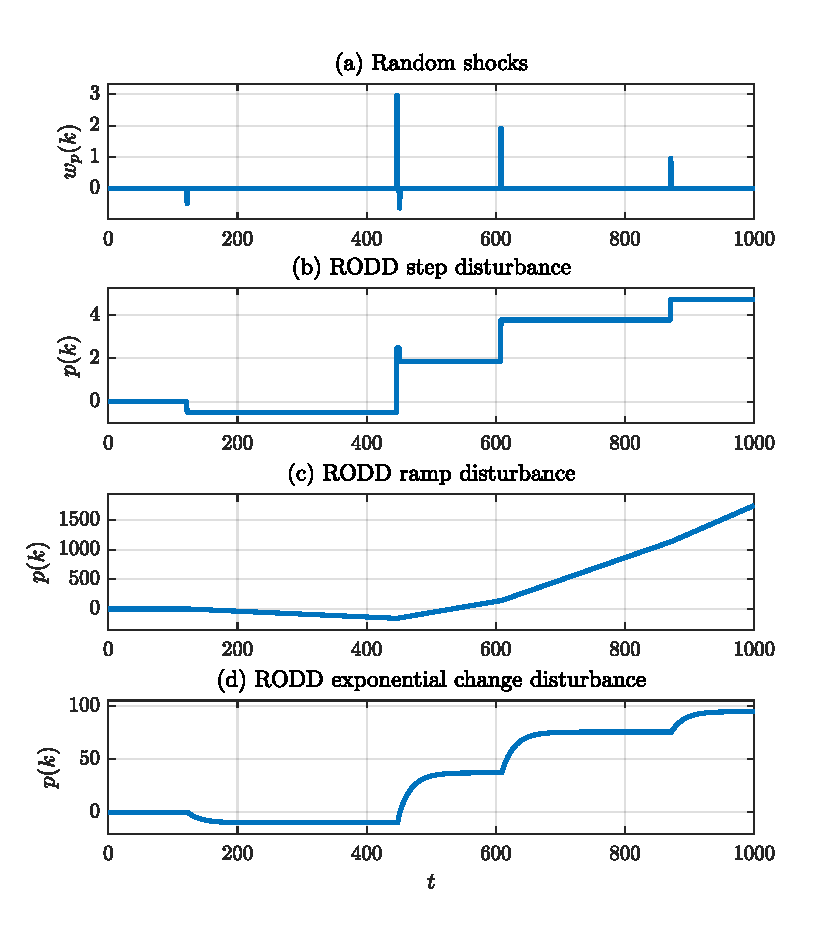
\includegraphics[width=13cm]{images/rodd_sim_plots.pdf}
	\caption{Examples of \gls{RODD}s}
	\label{fig:rodd-sim-plots}
\end{figure}
\begin{figure}[htp]
	\centering
	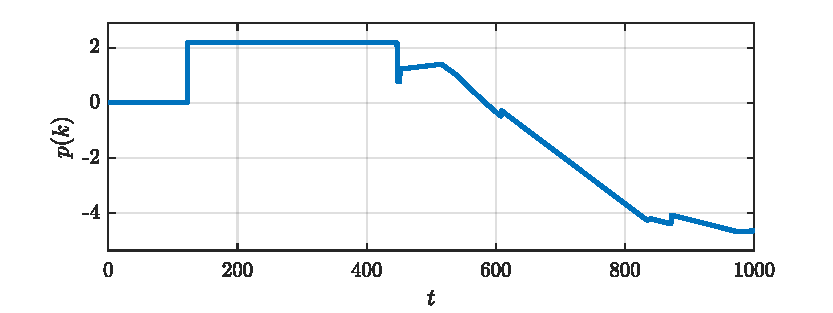
\includegraphics[width=13cm]{images/rodd_sim_plot2.pdf}
	\caption{A \gls{RODD} with steps and ramps}
	\label{fig:rodd-sim-plot2}
\end{figure}


\section{Observer evaluation with linear systems} \label{sec:sim-obs-lin}

\subsection{SISO linear system} \label{sec:sim-obs-lin-1}

To demonstrate state estimation in the presence of \gls{RODD}s, a single \gls{RODD} was simulated at the input to a SISO process represented by a discrete-time linear model, as shown in the functional diagram in Figure \ref{fig:sim-sys-diag-siso}. In addition to the unmeasured \gls{RODD}, $p(k)$, the process has a known input, $u(k)$, and a measured output, $y_M(k)$. The measurements are simulated by adding a random noise, $v(k)$, with zero mean and standard deviation, $\sigma_M$, to the output of the process. At each sample time, the input and measured output are passed to an observer, which calculates estimates of the process states, $\hat{\mathbf{x}}(k|k)$, and an estimate of the process output, $\hat{y}(k|k)$. % TODO: add glossary items for SISO variables.
\nomenclature{$\sigma_M$}{standard deviation of the measurement noise}
\begin{figure}[htp]
	\centering
	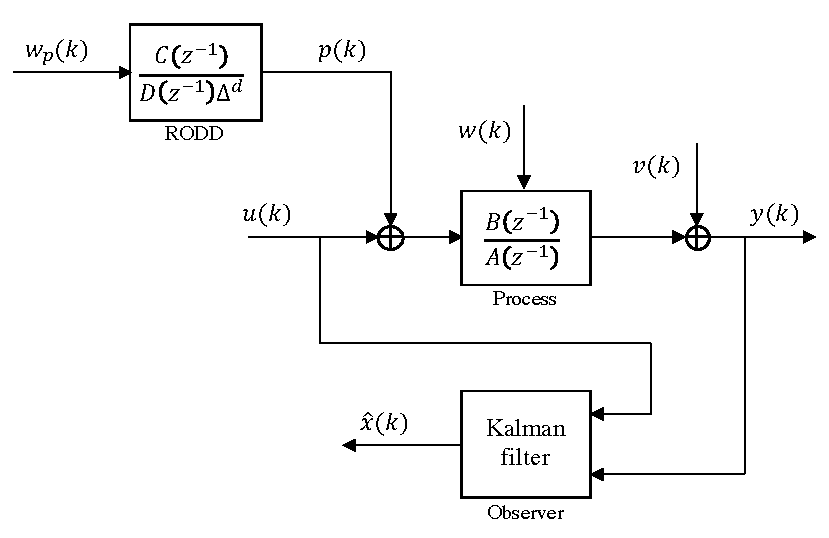
\includegraphics[width=11.5cm]{images/sim-sys-diag-siso.pdf}
	\caption{Functional diagram of the simulated \gls{SISO} system with observer}
	\label{fig:sim-sys-diag-siso}
\end{figure}

For the purposes of this experiment, the linear model used to represent the process was the stable first order system,
\begin{equation}
	\frac{B(q^{-1})}{A(q^{-1})} = \frac{0.3q^{-1}}{1-0.7q^{-1}}
\end{equation}
with a sampling period, $T_s$, of 0.5.
\nomenclature{$T_s$}{sampling interval in units of time}%

The \gls{RODD} was a step disturbance created by setting
\begin{equation}
	\frac{C(q^{-1})}{D(q^{-1})} = \frac{1}{1-q^{-1}}.
\end{equation}
The random shock, $w_p(k)$, was defined by \eqref{eq:wpik2} with $\varepsilon=0.01$, $\sigma_{w_p}=0.01$, and $b=100$.

The state-space model used to simulate the augmented system was
\begin{equation} \label{eq:sim-sys-siso-ss-aug}
	\begin{split}
	\mathbf{x}_{a}(k+1) & =\left[\begin{array}{cc}
		0.7 & 1 \\
		0 & 1
	\end{array}\right] \mathbf{x}_{a}(k)+\left[\begin{array}{l}
		1 \\
		0
	\end{array}\right] u(k) + \mathbf{w}_{a}(k) \\
	y_M(k) & =\left[\begin{array}{cc}
	0.3 & 0
\end{array}\right] \mathbf{x}_{a}(k) + v(k)
\end{split}
\end{equation}
where
\begin{equation} \label{eq:sim-sys-siso-ss-aug2}
		\mathbf{x}_{a}(k) = \left[\begin{array}{l}
			x_{a,1}(k) \\
			x_{a,2}(k)
		\end{array}\right] = \left[\begin{array}{l}
		x_{1}(k) \\
		p(k)
	\end{array}\right], \mathbf{w}_{a}(k) = \left[\begin{array}{l}
	w(k) \\
	w_{p}(k)
\end{array}\right] .
\end{equation}

Note that with this representation, the second model state $x_{a,2}(k)$ corresponds exactly to the input disturbance $p(k)$.

\subsection{Analysis of sub-optimal estimators} \label{sec:sim-obs-lin-1-SKF-analysis}

To understand and investigate the behaviour of the observers, the system \eqref{eq:sim-sys-siso-ss-aug} was first simulated for 100 sample periods with two pre-determined shocks, no persistent disturbance ($\sigma_{w_p}=0$), and no measurement noise ($\sigma_M=0$). Figure \ref{fig:rod-obs-sim-test-ioplot-SF95} shows the simulation data. The two lower plots show the system inputs, including the random shock signal. The upper two plots show the system states and outputs as well as the estimates of a sub-optimal multiple-model observer using the sequence fusion algorithm described by \cite{robertson_detection_1995} with parameters $N_f=15$, $n_\text{max}=1$, and $d=5$.
\begin{figure}[htp]
	\centering
	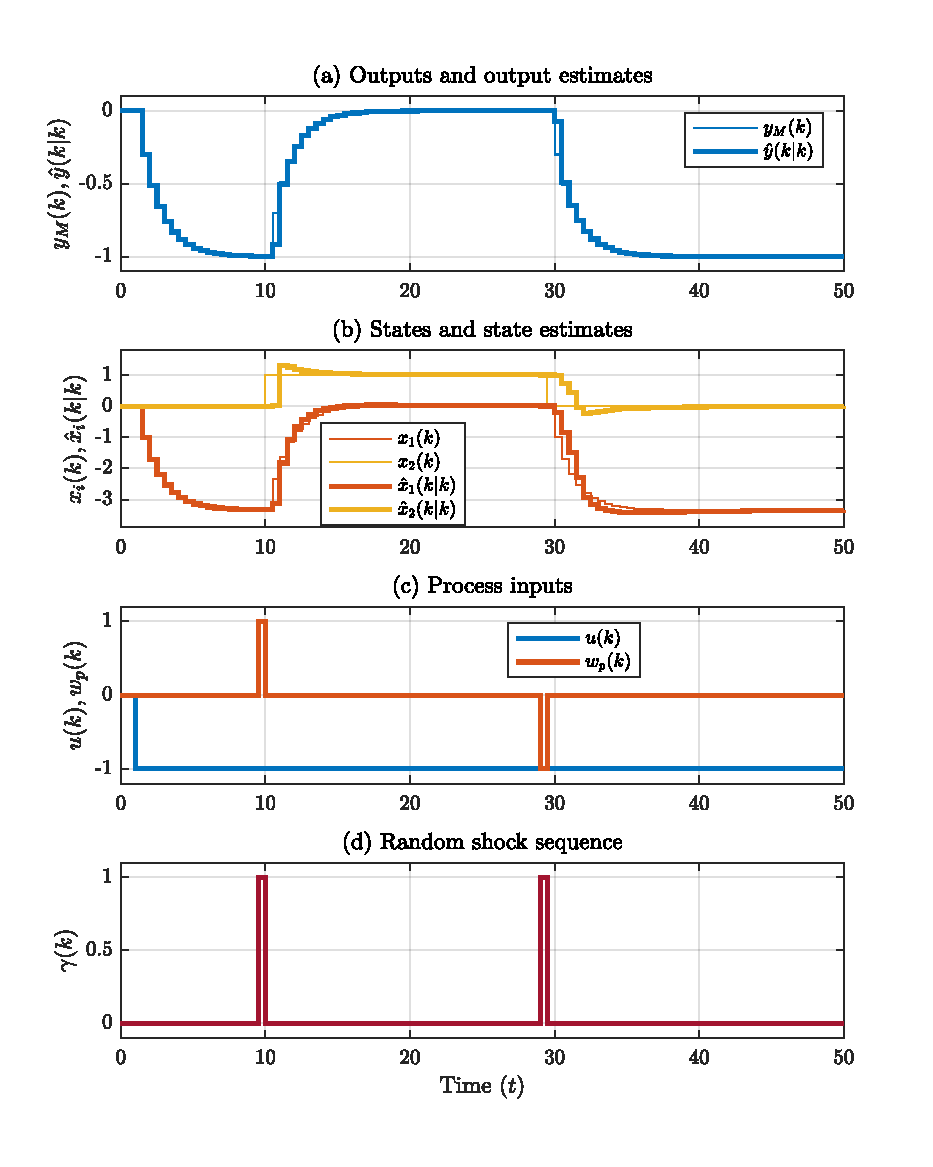
\includegraphics[width=13cm]{images/rod_MKF_SF_test_sim_MKF_SF95_ioplot.pdf}
	\caption{Simulation of a SISO linear system with a \gls{RODD} input disturbance}
	\label{fig:rod-obs-sim-test-ioplot-SF95}
\end{figure}

\begin{figure}[htp]
	\centering
	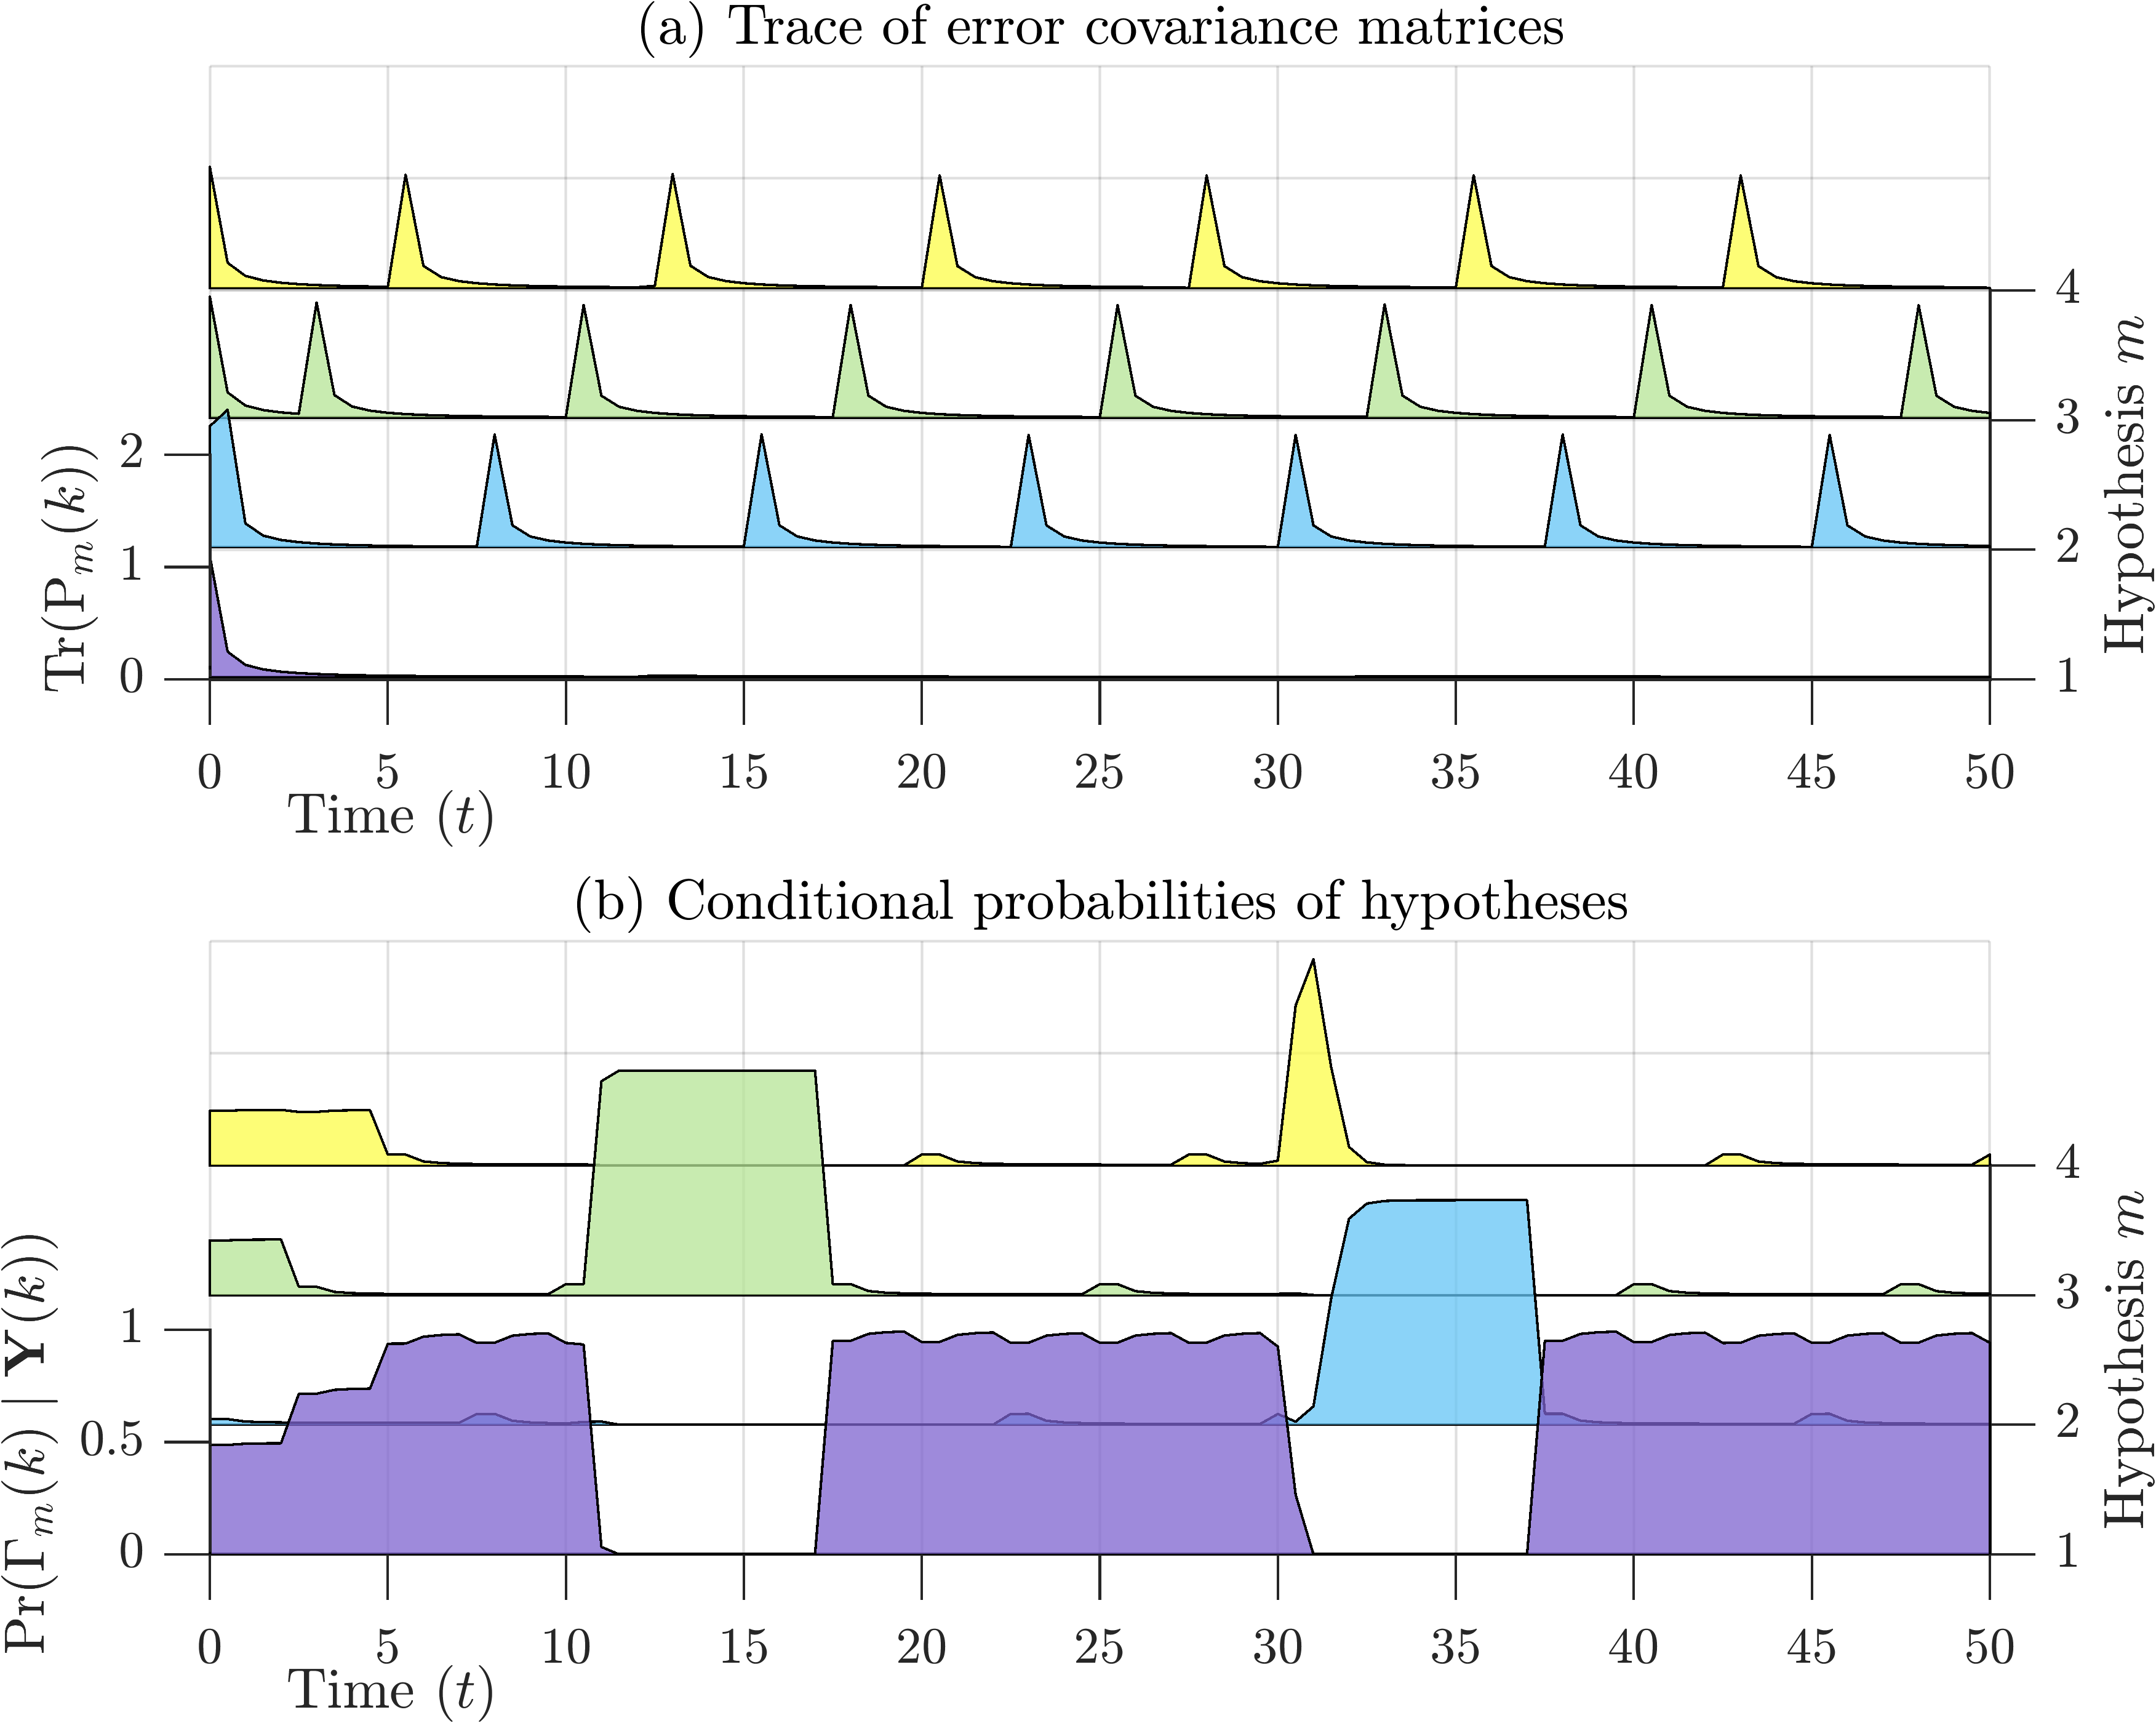
\includegraphics[width=12cm]{images/rod_MKF_test_sim_MKF_SF95_prob.png}
	\caption{Multi-model observer probability estimates – MKF--SF95}
	\label{fig:rod-obs-sim-test-probs-SF95}
\end{figure}
The two plots in Figure \ref{fig:rod-obs-sim-test-probs-SF95} provide insight into the computations of the observer, which is labelled `MKF--SF95'. The upper plot shows four time series of the trace (i.e. the sum of the elements on the main diagonal) of the merged error covariance matrices, $\mathbf{P}_m(k)$ for $m=1,2,...,n_m$. The diagonal values of $\mathbf{P}_m(k)$ may be interpreted as indicators of the magnitude of the errors of the state estimates. Recall that $\mathbf{P}_m(k)$ is time-varying and influenced by the process noise covariance, $\mathcal{Q}(\gamma_f(k))$, which switches according to the hypothesis sequences \eqref{eq:Pfkp1}. In this simulation, the covariances at time $t=0$ were initialized to the identity matrix ($\mathbf{P}_m(0)=\mathbf{I}_2$). It can be seen that the trace values initially drop rapidly and tend towards zero, however, at certain times, they increase sharply to a peak before dropping again. The sharp peaks are caused by the shock hypotheses ($\gamma_m(k)=1$) of the sequences.

The lower plot shows the conditional likelihood estimates of the four hypotheses given the data up to time $k$ after the merging step \eqref{eq:xmkymk_hat_MKF}. The conditional likelihoods were initialized with equal values ($\operatorname{Pr}\left(\Gamma_m(0) \mid \mathbf{Y}_M(0)\right)=1/n_m$). It can be seen that the likelihoods of each hypothesis settle on a steady-state by $t=5$ and hypothesis 1 dominates the probability distribution until $t=10$. This means that the merged estimates of the observer are determined almost completely by hypothesis 1 during this period. This makes sense since hypothesis 1 represents a sequence containing no shocks and the first shock does not occur until $t=9.5$. A short time after the first shock, the probability density shifts to hypothesis sequence 3 which happens to assume a shock at $t=10$. This is evident in the upper plot where it can be seen that the error covariance of hypothesis 3 increases and peaks at $t=10.5$. The probability switches from hypothesis 1 to 3 by $t=11.5$ and remains there until $t=17$ when it shifts back to hypothesis 1. This final shift can be explained by the fusion horizon, $N_f$, which in this case is 15 sample periods or 7.5 time units. Hypothesis 3 assumes another shock occurs at this time, which is not the case. Therefore, hypothesis 1 becomes the most likely hypothesis after that. The second shock occurs at $t=29$, which is not as favourable since it does not align well with the shocks in any of the hypothesis sequences. Initially, the likelihood switches to hypotheses 4, which assumes a shock at $t=27.5$ but then it switches to hypothesis 2, which assumes a shock at $t=30$. Again, the probability remains high until the next shock is scheduled, at which point hypothesis 1 becomes the most likely again.

\begin{figure}[htp]
	\centering
	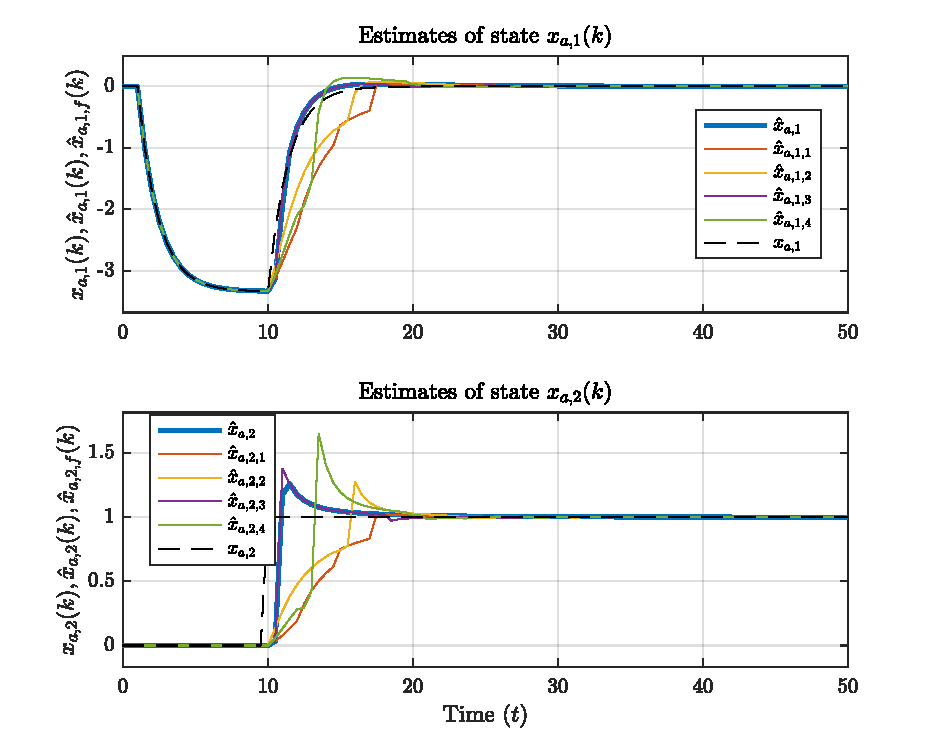
\includegraphics[width=13cm]{images/rod_MKF_test_sim_MKF_SF95_x_est.pdf}
	\caption{Multi-model observer state estimates – MKF--SF95}
	\label{fig:rod-obs-sim-test-x_est-SF95}
\end{figure}
Figure \ref{fig:rod-obs-sim-test-x_est-SF95} shows the merged state estimates associated with each hypothesis (thin coloured lines), as well as the overall state estimate (thick blue lines) and the true states of the system (dashed lines). These plots reveal the role that each hypothesis plays in the overall estimates. The estimates of hypothesis 3 (purple lines) are the first to respond to the first shock at time $t=9.5$ and the overall estimate closely follows this hypothesis. The other estimates (green, yellow and orange lines) respond at later intervals and do not play a role in the overall estimate. After the second shock occurs, the overall estimate follows that of hypothesis 4 at first, then it switches to 2, however, it lags the true system state and the response of the output estimate is slower and overshoots the true system output for a few time steps. These simulation results demonstrate that the performance of the sequence fusion algorithm is somewhat sensitive to the timing of the true shocks. Nevertheless, the output estimates are quite good and would likely be satisfactory in most process control applications. 

As described in Section \ref{sec:fusion}, Robertson and coworkers proposed an alternative implementation of the sequence fusion algorithm \citep{robertson_method_1998}. There are two differences between this and the previous algorithm. Firstly, shocks are assumed to act over the duration of the detection interval rather than at one sample time within it. Secondly, the variance of the shocks, $b^2\sigma_{w_p}^2$, is reduced according to the interval length \eqref{eq:wpdk}.
%% TODO: add parameters to above? with $f=15$ $m=1$ and $d=5$.

\begin{figure}[htp]
	\centering
	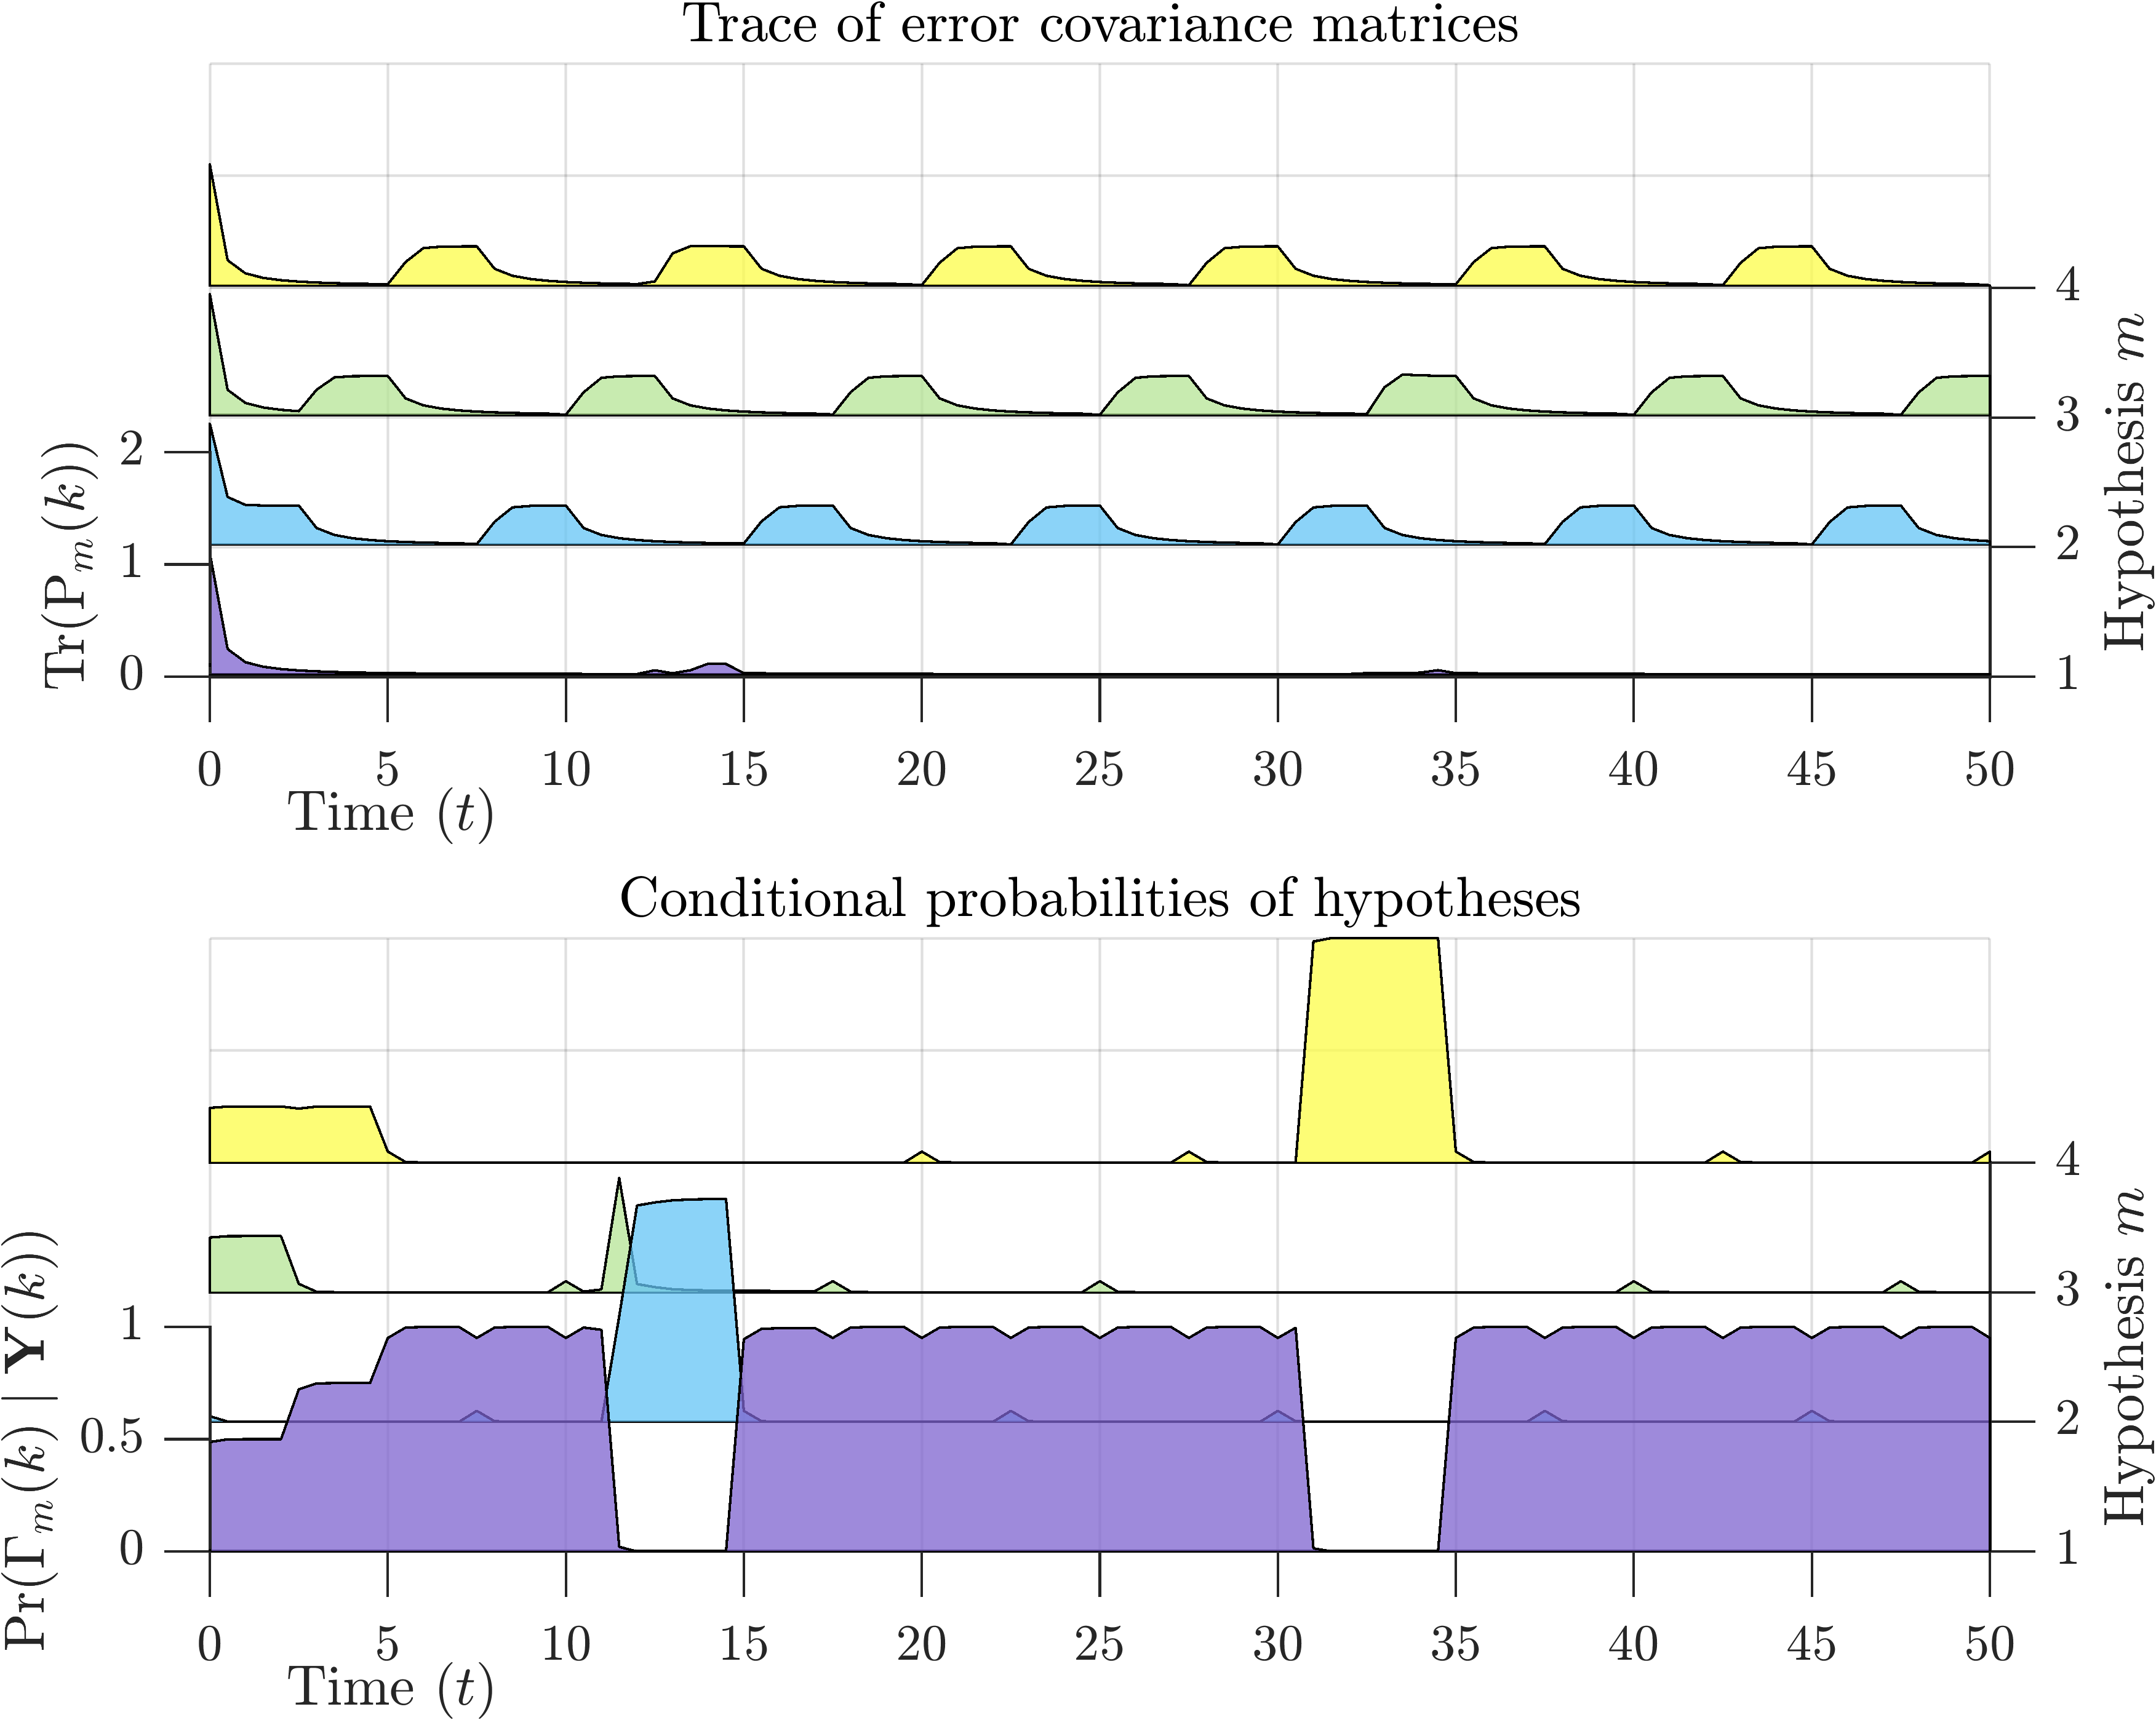
\includegraphics[width=12cm]{images/rod_MKF_test_sim_MKF_SF98_prob.png}
	\caption{Multi-model observer probability estimates – MKF--SF98}
	\label{fig:rod-obs-sim-test-probs-SF98}
\end{figure}
Figures \ref{fig:rod-obs-sim-test-probs-SF98} and \ref{fig:rod-obs-sim-test-x_est-SF98} show the results of simulating the 1998 version of the observer, labelled `MKF--SF98', with the same simulation data. The effect of the modifications on the error covariance is clear. The traces of the error covariance peak at a lower value and the peaks are sustained for the duration of the detection intervals, unlike in the 1995 version. The switching of the hypothesis probabilities is also different. After the first shock at $t=9.5$ the probability shifts to hypothesis 2 rather than 3. This may be due to the fact that the shock occurred in the middle of the detection interval of hypothesis 2. After the second shock at $t=29$ the hypothesis 4 becomes the most probable.

Figure \ref{fig:rod-obs-sim-test-x_est-SF98} shows the merged state estimates of each hypothesis, the overall estimates, and the true system states for the 1998 version of the algorithm. The estimates responding quickly to the shocks and there is noticeably less overshoot of the estimates in this simulation compared to the 1995 version.   
\begin{figure}[htp]
	\centering
	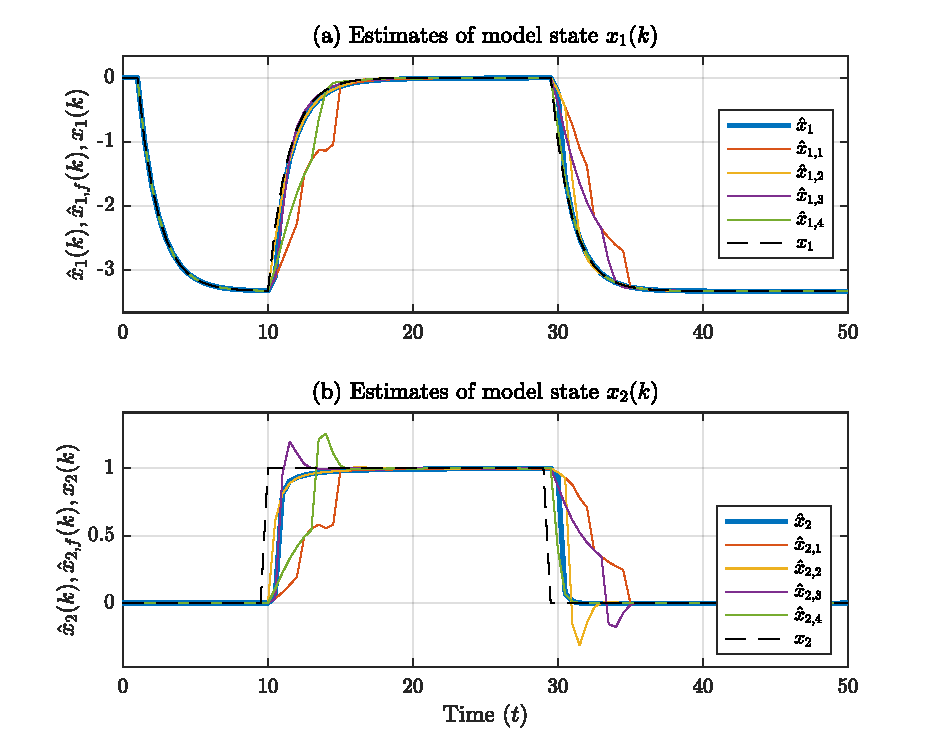
\includegraphics[width=13cm]{images/rod_MKF_test_sim_MKF_SF98_x_est.pdf}
	\caption{Multi-model observer state estimates – MKF--SF98}
	\label{fig:rod-obs-sim-test-x_est-SF98}
\end{figure}

\begin{figure}[htp]
	\centering
	\includegraphics[width=12cm]{images/rod_MKF_test_sim_MKF_SP_prob.png}
	\caption{Multi-model observer probability estimates – MKF--SP}
	\label{fig:rod-obs-sim-test-probs-SP}
\end{figure}
\begin{figure}[htp]
	\centering
	\includegraphics[width=13cm]{images/rod_MKF_test_sim_MKF_SP_x_est.pdf}
	\caption{Multi-model observer state estimates – MKF--SP}
	\label{fig:rod-obs-sim-test-x_est-SP}
\end{figure}
Figures \ref{fig:rod-obs-sim-test-probs-SP} and \ref{fig:rod-obs-sim-test-x_est-SP} show the corresponding results of simulating the sequence pruning multiple-model observer, labelled `MKF--SP', with $n_h=5$ and $N_\text{min}=2$, as described by \cite{eriksson_classification_1996}. Recall that in this algorithm, hypotheses are adaptively pruned and replaced at every sample time. From these plots it can be seen that the hypotheses include more possible shocks than those modelled by the sequence fusion observers with detection intervals. Also, the switching of hypothesis probabilities is swifter and distinct, and the estimation errors are visibly lower than those of both versions of the sequence fusion observer in these simulations.

To effectively evaluate and compare the performance of these observers, longer simulations with pseudo-random shocks and measurement noise are needed. Figure \ref{fig:rod-obs-sim1-ioplot} shows the first 600 input-output samples from a simulation of the system with a total duration of 2500 (5000 samples). The lower plot shows the input signals, $u(k)$ and $p(k)$, from which it can be seen that two significant random shocks occurred during this period (at $t=98$ and $220.5$). At other times, the value of $p(k)$ is a random walk due to the persistent component of the \gls{RODD} disturbance \eqref{eq:wpk2}. In addition, a step change in $u(k)$ of magnitude 1 occurred at time $t=5$. The upper plot shows the simulated output measurements. The standard deviation of the measurement noise, $\sigma_M$, was $0.1$. No disturbances other than $w_p(k)$ were simulated (i.e. $w_1(k)=0$).
\begin{figure}[htp]
	\centering
	\includegraphics[width=13cm]{images/rod_obs_sim1_all_seed_ioplot.pdf}
	\caption{Simulation of linear system with a \gls{RODD} input disturbance}
	\label{fig:rod-obs-sim1-ioplot}
\end{figure}

\subsubsection{Tuning of Kalman filters} \label{sec:sim-obs-lin-1-KF-tuning}

Standard Kalman filters were used to develop performance baselines with which to evaluate the sub-optimal multiple-model observers. The question of how to set the gain of a Kalman filter when there is a \gls{RODD} affecting the system is open to interpretation. One naive approach is to tune the Kalman filter using the variance of the persistent component of the disturbance, $\sigma_{w_p}^2$, if it is known. In this case, the Kalman filter, which is labelled `KF1', has a noise covariance matrix
\nomenclature{$\mathbf{Q}_0$}{noise covariance matrix used in observer simulations}%
\begin{equation} \label{eq:sim-sys-siso-KF1-Q}
	\begin{aligned}
		\mathbf{Q}_{\text{KF1}}=\mathbf{Q}_0=\begin{bmatrix}
			\sigma_{x}^2 & 0 \\
			0 &  \sigma_{w_p}^2 \\
		\end{bmatrix}=\begin{bmatrix}
		0.1^2 & 0 \\
		0 & 0.01^2 \\
	\end{bmatrix}
	\end{aligned},
\end{equation}
\nomenclature{$\sigma_{x}^2$}{variance of the errors of the process model state(s)}
where $\sigma_{x}^2$ is a parameter representing the variance of the errors of the process model state, $x(k)$. However, this leads to a filter with a slow response to shocks. The choice of $\sigma_{x}=0.1$ was somewhat arbitrary. In these simulations, the process is simulated by a model that is identical to the model used by the observers, so there is no model error in steady-state. However, in transient periods such as after a shock disturbance, and in real applications, errors between the observer model and the true states are expected.

A second option is to tune a Kalman filter to the variance of the infrequent shocks, $b^2\sigma_{w_p}^2$.  In this case, the Kalman filter, labelled `KF2', has a state disturbance covariance
\nomenclature{$\mathbf{Q}_1$}{noise covariance matrix used in observer simulations}%
\begin{equation} \label{eq:sim-sys-siso-KF2-Q}
	\begin{aligned}
		\mathbf{Q}_{\text{KF2}}=\mathbf{Q}_1=\begin{bmatrix}
			\sigma_{x}^2 & 0 \\
			0 & b^2\sigma_{w_p}^2 \\
		\end{bmatrix}=\begin{bmatrix}
			0.1^2 & 0 \\
			0 & 1^2 \\
		\end{bmatrix}.
	\end{aligned}
\end{equation}
The problem with this filter is that it is very sensitive to the measurement noise, $v(k)$. 

As explained by \cite{andersson_adaptive_1985} and \cite{robertson_detection_1995}, a trade-off is needed. One approach to making this trade-off is to minimize the average estimation errors over a suitably long set of input-output data. In this case, 5000 samples were generated from the simulated system (\ref{fig:sim-sys-diag-siso}) and then a Kalman filter was simulated multiple times, each time with a different tuning. 
\begin{figure}[htp]
	\centering
	\includegraphics[width=13cm]{images/rod_obs_sim1_3KF_Q_seed_6.pdf}
	\caption{Tuning of Kalman filter KF3 – SISO system}
	\label{fig:sim-sys-siso-KF3-tuning}
\end{figure}
Figure \ref{fig:sim-sys-siso-KF3-tuning} shows the results of these simulations, from which it can be seen that the lowest \gls{RMSE}s of the state estimates were achieved when the variance parameter $\sigma_{w_p}^2$ was close to $0.01$. Using this result, a third Kalman filter labelled `KF3' was designed with the state disturbance covariance matrix
\nomenclature{$\mathbf{Q}_{\text{opt}}$}{noise covariance matrix used in the Kalman filter tuned to minimize overall \gls{RMSE} of the output estimates}%
\begin{equation} \label{eq:sim-sys-siso-KF3-Q}
	\begin{aligned}
		\mathbf{Q}_{\text{KF3}}=\mathbf{Q}_{\text{opt}}=\begin{bmatrix}
			\sigma_{x}^2 & 0 \\
			0 & \sigma_{w_p,\text{opt}}^2 \\
		\end{bmatrix}=\begin{bmatrix}
			0.1^2 & 0 \\
			0 & 0.1^2 \\
		\end{bmatrix}.
	\end{aligned}
\end{equation}

Figure \ref{fig:sim-sys-siso-KF123-est} shows the estimates of the three Kalman filters described above when simulated on the input-output data. The upper plot shows the output estimates and the lower plot shows the estimates of the model state $x_{a,2}(k)$, which corresponds to the estimate of the \gls{RODD}, $p(k)$. As expected, the response of KF1 to the infrequent step disturbances is noticeably slower than that of the other two. The response of KF2 is fast, but it is sensitive to the measurement noise. KF3 is a compromise between the two—a relatively fast response to the infrequent steps and less sensitivity to the measurement noise.
\begin{figure}[htp]
	\centering
	\includegraphics[width=13cm]{images/rod_obs_sim1_all_seed_y_est1_KF123.pdf}
	\caption{Kalman filter estimates}
	\label {fig:sim-sys-siso-KF123-est}
\end{figure}

One way to visualise the observer performance is to plot the square of the output estimation errors, which are the differences between the estimates, $\hat{y}(k \mid k)$, and the true values of the system outputs, $y(k)$. The upper plot in Figure \ref{fig:sim-sys-siso-KF123-cumerr} shows the squared errors in the output estimates of the three Kalman filters. The lower plot shows the cumulative sum of the squared errors. This clearly shows the differences in performance. The estimation errors of KF1 are small when the system is in steady-state but increase dramatically after each step disturbance. The magnitude of the errors of KF2 during steady-state periods is high but roughly constant throughout the simulation. KF3 achieves the lowest overall cumulative sum-of-squared-errors by the end of the simulation.
\begin{figure}[htp]
	\centering
	\includegraphics[width=13cm]{images/rod_obs_sim1_all_seed_cum_err_y1_KF123.pdf}
	\caption{Cumulative errors of Kalman filter estimates}
	\label{fig:sim-sys-siso-KF123-cumerr}
\end{figure}

The RMSEs of the state estimates in these simulations are shown in Figure \ref{fig:rod-obs-sim1-KF123-xest-RMSE-bar}. These plots show the total RMSEs divided into two components. The blue part, labelled `no noise' is the RMSE when the system was simulated without measurement noise, (i.e. $y_M(k)=y(k)$). The orange part, labelled `due to noise' represents the difference in the RMSE between simulating with measurement noise and without. This distinction is only possible with a simulation model---in real applications it is not possible to obtain the true system outputs.
\begin{figure}[htp]
	\centering
	\includegraphics[width=12cm]{images/rod_obs_sim1_all_seed_x_err_bar_KF123.pdf}
	\caption{Root-mean-squared errors of state estimates – SISO system}
	\label{fig:rod-obs-sim1-KF123-xest-RMSE-bar}
\end{figure}

As well as allowing the overall RMSE values of the three Kalman filters to be compared, these plots also illustrate the relative magnitudes of the sources of the error. As expected, the errors of KF1 are almost all due to its slow dynamic response to the shocks, whereas very little is due to the measurement noise. The opposite is true of KF2, which has a very fast dynamic response to the shocks. The trade-off between the two sources of errors is clearly illustrated for KF3. It should be noted that this may not be the best trade-off in every case. In some applications, the speed of response may be more important than the sensitivity to noise, or vice-versa. The trade-off resulting from minimizing the overall RMSE is used in this work.

\subsubsection{Selection of multiple-model observer parameters} \label{sec:sim-obs-lin-1-MKF-tuning}

Parameter values for the sub-optimal multiple-model observer algorithms described in Section \ref{sec:fusion} were chosen by a similar method. The sequence fusion algorithms proposed by \cite{robertson_detection_1995} and \cite{robertson_method_1998} have three parameters, $N_f$, $n_\text{max}$, and $d$. Candidate values for these parameters were generated by considering every combination satisfying

\begin{equation} \label{eq:sim-sys-siso-MKF-SF-param-values}
	\begin{aligned}
		\frac{N_f}{N_d} &\in \left\{3, 5, 10, 15, 20\right\},  \\
		n_\text{max} &\in \left\{1, 2, 3\right\},  \\
		N_d &\in \left\{1, 2, 3, 5, 10\right\}.
	\end{aligned}
\end{equation}

Note that $\frac{N_f}{d}$ represents the number of detection intervals within the fusion horizon and is always a whole number. For example, when $d=3$, the lengths of the fusion were 9, 15, 30, 45, and 60. However, not all combinations were simulated. Any combination with more than 200 hypotheses ($n_h>200$) or with a total probability modelled, $\beta$ \eqref{eq:p_gamma}, less than 0.85 was rejected. The remaining 58 combinations were then evaluated by simulating the observer and calculating the \gls{RMSE} of the output estimates on the 5000 data samples from the simulated system. Tables \ref{tb:obs-sim1-popt-SF95} and \ref{tb:obs-sim1-popt-SF98} show the resulting \gls{RMSE} results for the 10 best combinations of parameter values (those with the lowest output \gls{RMSE}) for the 1995 and 1998 variants of this algorithm.
\begin{table}[ht]
	\begin{center}
		\caption{Multi-model observer parameter search results – MKF--SF95.} \label{tb:obs-sim1-popt-SF95}
		% See: https://texblog.org/2019/06/03/control-the-width-of-table-columns-tabular-in-latex/
		\begin{tabular}{p{0.05\textwidth}>{\centering\arraybackslash}p{0.07\textwidth}>{\centering\arraybackslash}p{0.07\textwidth}>{\centering\arraybackslash}p{0.07\textwidth}>{\centering\arraybackslash}p{0.07\textwidth}>{\centering\arraybackslash}p{0.15\textwidth}}
			$N_f$ & $n_\text{max}$ & $d$ & $n_h$ & $\beta$ & $\text{\gls{RMSE}}(\hat{Y},Y)$  \\
			\hline
			% See script rod_obs_sim1_MKF_SF95_popt_table.m
			% 29-Nov-2022 18:35:37 results with seed = 6, sigma_M = 0.1, d_min = 1
			15 &   2 &   1 & 151 & 0.9996 & 0.0411 \\
			20 &   2 &   1 & 251 & 0.9990 & 0.0411 \\
			10 &   2 &   1 &  76 & 0.9999 & 0.0411 \\
			10 &   3 &   1 & 268 & 1.0000 & 0.0411 \\
			5 &   1 &   1 &   8 & 0.9990 & 0.0415 \\
			5 &   2 &   1 &  26 & 1.0000 & 0.0415 \\
			5 &   3 &   1 &  48 & 1.0000 & 0.0415 \\
			15 &   1 &   1 &  18 & 0.9904 & 0.0418 \\
			10 &   1 &   1 &  13 & 0.9957 & 0.0419 \\
			10 &   2 &   2 &  16 & 0.9043 & 0.0426 \\
			\hline
		\end{tabular}
	\end{center}
\end{table}
\begin{table}[ht]
	\begin{center}
		\caption{Multi-model observer parameter search results – MKF--SF98.} \label{tb:obs-sim1-popt-SF98}
		% See: https://texblog.org/2019/06/03/control-the-width-of-table-columns-tabular-in-latex/
		\begin{tabular}{p{0.05\textwidth}>{\centering\arraybackslash}p{0.07\textwidth}>{\centering\arraybackslash}p{0.07\textwidth}>{\centering\arraybackslash}p{0.07\textwidth}>{\centering\arraybackslash}p{0.07\textwidth}>{\centering\arraybackslash}p{0.15\textwidth}}
			$N_f$ & $n_\text{max}$ & $d$ & $n_h$ & $\beta$ & $\text{\gls{RMSE}}(\hat{Y},Y)$  \\
			\hline
			% See script rod_obs_sim1_MKF_SF98_popt_table
			% 29-Nov-2022 18:38:45 results with seed = 6, sigma_M = 0.1, d_min = 1
%			15 &   2 &   1 & 151 & 0.9996 & 0.0411 \\
%			20 &   2 &   1 & 251 & 0.9990 & 0.0411 \\
%			10 &   2 &   1 &  76 & 0.9999 & 0.0411 \\
%			10 &   3 &   1 & 268 & 1.0000 & 0.0411 \\
%			5 &   1 &   1 &   8 & 0.9990 & 0.0415 \\
%			5 &   2 &   1 &  26 & 1.0000 & 0.0415 \\
%			5 &   3 &   1 &  48 & 1.0000 & 0.0415 \\
%			15 &   1 &   1 &  18 & 0.9904 & 0.0418 \\
%			10 &   1 &   1 &  13 & 0.9957 & 0.0419 \\
%			20 &   1 &   1 &  23 & 0.9831 & 0.0429 \\
			% See script rod_obs_sim1_MKF_SF98_popt_table.m
			% 07-Dec-2022 23:56:27 results with seed = 6, sigma_M = 0.1, d_min = 1
			30 &   2 &   2 & 151 & 0.9970 & 0.0414 \\
			20 &   2 &   2 &  76 & 0.9991 & 0.0414 \\
			10 &   2 &   2 &  26 & 0.9999 & 0.0414 \\
			10 &   3 &   2 &  48 & 1.0000 & 0.0414 \\
			6 &   1 &   2 &   6 & 0.9988 & 0.0414 \\
			6 &   2 &   2 &  13 & 1.0000 & 0.0414 \\
			6 &   3 &   2 &  16 & 1.0000 & 0.0414 \\
			10 &   1 &   2 &   8 & 0.9962 & 0.0416 \\
			9 &   1 &   3 &   6 & 0.9974 & 0.0418 \\
			9 &   2 &   3 &  13 & 1.0000 & 0.0418 \\
			\hline
		\end{tabular}
	\end{center}
\end{table}

From a practical standpoint, it is not desirable to simulate a large number of hypotheses. On this basis, the third combination in Table \ref{tb:obs-sim1-popt-SF95} ($N_f=10,n_\text{max}=2,d=1$, requiring 76 hypotheses) or the fifth ($N_f=5,n_\text{max}=1,d=1$, requiring only 8 hypotheses) are good choices for the 1995 version. The fifth combination was chosen for the simulations and the observer was labelled `MKF--SF95'. 

In terms of overall estimation errors, the two sequence fusion algorithms are very similar. Note that in the case of the 1998 version, it produces identical results to the MKF--SF95 observer when the spacing parameter $d$ is 1. The differences between the two algorithms are only in the way the estimates are updated during the steps of the detection interval. Therefore, results for the 1998 algorithm with $d=1$ were discarded. \cite{robertson_method_1998} state that the approach is a means of obtaining a long detection horizon, which is necessary when many sampling intervals are required to discriminate among multiple abrupt changes that may occur. Since in this simulation there is only one \gls{RODD} disturbance, and the best results were achieved with a detection interval of 1, it was concluded that these features of the 1998 algorithm were not applicable to this problem.

Nevertheless, based on the results in Table \ref{tb:obs-sim1-popt-SF98}, an observer labelled `MKF--SF1' was selected for simulation with $N_f=6$, $n_\text{max}=1$, and $d=2$. This requires only 6 hypotheses and achieves as good a performance as `MKF--SF95'.

The sequence pruning algorithm proposed by \cite{eriksson_classification_1996} has two parameters that must be specified, $n_h$, and $N_\text{min}$. Candidate values for these parameters were generated by considering all combinations satisfying

\begin{equation} \label{eq:sim-sys-siso-MKF-SP-param-values}
	\begin{aligned}
		n_h &\in \left\{3, 4, 5, 7, 10, 14, 19, 25, 32\right\},  \\
		N_\text{min} &\in \left\{1, 2, 3, 4, 5, 6, 7, 9, 12, 16, 21\right\}.
	\end{aligned}
\end{equation}

Combinations where rejected when $n_h - N_\text{min} < 1$, or in other words, when the minimum life, $N_\text{min}$, was greater than or equal to the number of hypotheses, $n_h$. This is a necessary condition since there must be enough filters to simulate the hypotheses until they reach the minimum life. Each remaining combination was then evaluated in the same way by calculating the \gls{RMSE} of the output estimates on the same 5000 samples used in the tuning of the sequence fusion observers described above. Table \ref{tb:obs-sim1-popt-SP} shows the top 10 combinations of parameter values in terms of lowest \gls{RMSE}.

\begin{table}[ht]
	\begin{center}
		\caption{Multi-model observer parameter search results – MKF--SP.} \label{tb:obs-sim1-popt-SP}
		% See: https://texblog.org/2019/06/03/control-the-width-of-table-columns-tabular-in-latex/
		\begin{tabular}{p{0.05\textwidth}>{\centering\arraybackslash}p{0.07\textwidth}>{\centering\arraybackslash}p{0.15\textwidth}}
			$n_h$ & $N_\text{min}$ & $\text{\gls{RMSE}}(\hat{Y},Y)$  \\
			\hline
			% See script rod_obs_sim1_MKF_SP_popt_table.m
			% 29-Nov-2022 18:24:40 results with seed = 6, sigma_M = 0.1
			10 &   7 & 0.0409  \\
			10 &   6 & 0.0410  \\
			19 &  16 & 0.0411  \\
			14 &  12 & 0.0411  \\
			25 &  21 & 0.0411  \\
			14 &   7 & 0.0411  \\
			19 &   7 & 0.0412  \\
			19 &   6 & 0.0412  \\
			25 &  16 & 0.0412  \\
			25 &  12 & 0.0412  \\
			\hline
		\end{tabular}
	\end{center}
\end{table}

As above, the differences between the \gls{RMSE}s of the best 10 combinations are small, indicating that the choice of parameters from these combinations is not critical. The first combination ($n_h=10,N_\text{min}=7$) was chosen and the observer was labelled `MKF--SP1' in the simulations below. Table \ref{tb:obs-params-sim1} is a summary of the parameters of the observers simulated.
\begin{table}[ht]
	\begin{center}
		\caption{Observer parameters for \gls{SISO} linear system.} \label{tb:obs-params-sim1}
		% See: https://texblog.org/2019/06/03/control-the-width-of-table-columns-tabular-in-latex/
		\begin{tabular}{p{0.16\textwidth}>{\centering\arraybackslash}p{0.12\textwidth}>{\centering\arraybackslash}p{0.16\textwidth}>{\centering\arraybackslash}p{0.16\textwidth}>{\centering\arraybackslash}p{0.16\textwidth}}
			& KF3 & MKF--SF95 & MKF--SF1 & MKF--SP \\
			\hline
			Type & Kalman filter & Multi-model Kalman filter & Multi-model Kalman filter & Multi-model Kalman filter \\
			Algorithm & - & Sequence fusion 95 & Sequence fusion 98 & Sequence pruning \\
			\hline
			Parameters &  &  &  &  \\
			$\mathcal{Q}$ & $\mathbf{Q}_{opt}$ & $\{\mathbf{Q}_0,\mathbf{Q}_1\}$ & $\{\mathbf{Q}_0,\mathbf{Q}_1\}$ & $\{\mathbf{Q}_0,\mathbf{Q}_1\}$ \\
			$\mathbf{R}$ & $0.1^2$ & $0.1^2$ & $0.1^2$ & $0.1^2$ \\
			$\mathbf{P}(0)$ & $\mathbf{P}_0$ & $\mathbf{P}_0$ & $\mathbf{P}_0$ & $\mathbf{P}_0$ \\
			$n_h$ & 1 & 8 & 6 & 10 \\
			$N_f$ & - & 5 & 6 & - \\
			$n_\text{max}$ & - & 1 & 1 & - \\
			$d$ & - & 1 & 2 & - \\
			$N_\text{min}$ & - & - & - & 7 \\
			$\varepsilon$ & - & 0.01 & 0.01 & 0.01 \\
			$\sigma_{w_p}$ & - & 0.01 & 0.01 & 0.01 \\
			$b$ & - & 100 & 100 & 100 \\
			\hline
		\end{tabular}
	\end{center}
\end{table}

\subsubsection{Scheduled Kalman filter} \label{sec:sim-obs-lin-1-SKF}

To determine the best performance that could be achieved by an ideal multiple-model observer, a hypothetical observer that has access to the true shock indicator signal, $gamma_k$, was simulated. This `scheduled' Kalman filter, labelled ‘SKF’, has only one shock sequence---the correct one---and therefore the process noise covariance is automatically switched to match the known shock signal. The \gls{SKF} is hypothetical because it could not be implemented in a real application where the random shocks are not known.

\subsubsection{Simulation results} \label{sec:sim-obs-lin-1-results}

Figure \ref{fig:rod-obs-sim1-yest-1-SF} shows the estimates of the sequence fusion observers, MKF--SF95 and MKF--SF1, compared to the scheduled Kalman Filter, \gls{SKF}, over the first 600 time steps of the simulation. From these results it is apparent that the estimates of the sequence fusion observers are generally very close to those of the \gls{SKF}. The estimates respond quickly when the random shocks occur and their variance at other times is relatively small despite the measurement noise. A few spontaneous errors of short duration are also noticeable in both the \gls{SKF} and MKF--SF1 estimates at certain times. However, when the variances are compared to those of the Kalman filters in Figure \ref{fig:sim-sys-siso-KF123-est}, it is clear that these multiple-model observers have an advantage.
\begin{figure}[htp]
	\centering
	\includegraphics[width=13cm]{images/rod_obs_sim1_all_seed_y_est1_SF95_SF1.pdf}
	\caption{Estimates by sequence fusion observers – \gls{SISO} system}
	\label{fig:rod-obs-sim1-yest-1-SF}
\end{figure}

Figure \ref{fig:rod-obs-sim1-yest-1-SP} shows the estimates of the sequence pruning observer, MKF--SP1, compared to the scheduled Kalman Filter. It also responds quickly to the shocks and is insensitive to the measurement noise, similar to the sequence fusion observers.
\begin{figure}[htp]
	\centering
	\includegraphics[width=13cm]{images/rod_obs_sim1_all_seed_y_est1_SP1.pdf}
	\caption{Estimates by sequence pruning observer – \gls{SISO} system}
	\label{fig:rod-obs-sim1-yest-1-SP}
\end{figure}

The plots in Figure \ref{fig:rod-obs-sim1-cum-err-y1-all} show the squared output errors and the cumulative squared-errors of the five observers over the full duration of the simulation. The differences between the multiple-model observers are almost indistinguishable. By the end of the simulation, the cumulative errors are significantly lower than those of KF3 and slightly higher than the \gls{SKF}.
\begin{figure}[htp]
	\centering
	\includegraphics[width=13cm]{images/rod_obs_sim1_all_seed_cum_err_y1.pdf}
	\caption{Cumulative errors of observer estimates – SISO system}
	\label{fig:rod-obs-sim1-cum-err-y1-all}
\end{figure}

Figure \ref{fig:rod-obs-sim1-xest-RMSE-bar} compares the \gls{RMSE}s of the state estimates of the five observers over the full simulation. From this, it can be seen that the multiple-model observers achieve lower \gls{RMSE}s than KF3, both in simulations with and without noise. The reduction in the errors due to the lower sensitivity to measurement noise (orange bars) is a more significant contribution to the improved performance of the multiple-model observers. It is noteworthy that most of the errors in the estimates of state 2, which corresponds to the input disturbance, are not due to measurement noise. This may partly be attributed to the delay in the process, which makes it impossible for the observers to immediately detect an unmeasured disturbance. They are also due to errors in tracking the persistent component of the disturbance, which can be seen in Figures \ref{fig:rod-obs-sim1-yest-1-SF} and \ref{fig:rod-obs-sim1-yest-1-SP}.
\begin{figure}[htp]
	\centering
	\includegraphics[width=12cm]{images/rod_obs_sim1_all_seed_x_err_bar.pdf}
	\caption{Root-mean-squared errors of state estimates – \gls{SISO} system}
	\label{fig:rod-obs-sim1-xest-RMSE-bar}
\end{figure}

Because these processes are stochastic, it is important to run simulations of sufficient duration to be confident that the results are representative of average performance. Figure \ref{fig:rod-obs-sim1-yest-all-seed-RMSE-box} provides an indication of the sensitivity of the \gls{RMSE} results to the initialization of the pseudo-random number generator used in these simulations. The data for this figure are from the results of 10 simulations, each of 5000 samples and each with a different pseudo-random initialization. It can be seen that the \gls{RMSE} values are somewhat sensitive to the random initialization but the variation is an order of magnitude lower than the difference between the multiple-model observers and KF3.
\begin{figure}[htp]
	\centering
	\includegraphics[width=12cm]{images/rod_obs_sim1_all_seed_y_err_box.pdf}
	\caption{Sensitivity of output estimation errors to random initialization – SISO system}
	\label{fig:rod-obs-sim1-yest-all-seed-RMSE-box}
\end{figure}
Figure \ref{fig:rod-obs-sim1-yest-all-seed-RMSE-box} confirms that the multiple-model observers are a significant improvement on the best single Kalman filter. However, there is no significant difference between the \gls{MKF}s in this case.
% Plots for analysis of SF performance
%
%\begin{figure}[htp]
%	\centering
%	\includegraphics[width=15cm]{images/rod-obs-sim-1-4-wfplot-DRAFT.png}
%	\caption{Evolution of conditional probabilities with sequence fusion}
%	\label{fig:rod-obs-sim1-4-wfplot}
%\end{figure}
%
%\begin{figure}[htp]
%	\centering
%	\includegraphics[width=14cm]{images/rod-obs-sim-1-4-est-MKF-SF-plot-DRAFT.pdf}
%	\caption{Filter estimates of sequence fusion observer during step disturbances}
%	\label{fig:rod-obs-sim1-4-est-MKF-SF-plot-DRAFT}
%\end{figure}
%
%\begin{figure}[htp]
%	\centering
%	\includegraphics[width=14cm]{images/rod_obs_sim2_7_mse_ashocks.pdf}
%	\caption{Average errors of observer estimates after shock disturbances}
%	\label{fig:rod_obs_sim2_7_mse_ashocks}
%\end{figure}

\subsection{MIMO linear system} \label{sec:sim-obs-lin-2}

\cite{robertson_method_1998} stated that in the case of more than one \gls{RODD} disturbance, it often takes many sampling intervals to discriminate among possible disturbances. The main motivation for the detection intervals used in their approach was to achieve a longer \textit{detection horizon} without requiring a very large number of hypotheses. To evaluate this feature, a \gls{MIMO} system with a 2-input, 2-output ($2\times2$) process model was chosen. The system has two independent \gls{RODD} step disturbances added to each manipulated input, as shown in the functional diagram in Figure \ref{fig:sim-sys-diag-2x2}. 
\begin{figure}[htp]
	\centering
	\includegraphics[width=11.5cm]{images/sim-sys-diag-2x2.pdf}
	\caption{Functional diagram of the simulated MIMO system}
	\label{fig:sim-sys-diag-2x2}
\end{figure}

The process model is a discrete-time linear model derived from the $2\times2$ continuous-time system,
% 2x2 system #1 - see sys_rodin_step_2x2sym.m
%\begin{equation} \label{eq:sim-sys-mimo-ct}
%	\mathbf{G}(s) = \left[\begin{array}{cc}
%		G_{11}(s) & G_{12}(s)  \\
%		G_{21}(s) & G_{22}(s)  \\
%	\end{array}\right] = \left[\begin{array}{cc}
%		\frac{1}{1+8.5s} & \frac{-0.5}{1+8.5s}  \\
%		\frac{-0.5}{1+8.5s} & \frac{1}{1+8.5s}  \\
%	\end{array}\right]
%\end{equation}
% 2x2 system #2 - see sys_rodin_step_2x2sym2.m
\begin{equation} \label{eq:sim-sys-mimo-ct}
	\mathbf{G}(s) = \left[\begin{array}{cc}
		G_{11}(s) & G_{12}(s)  \\
		G_{21}(s) & G_{22}(s)  \\
	\end{array}\right] = \left[\begin{array}{cc}
		\frac{1}{1+8.5s} & \frac{0.5}{1+8.5s}  \\
		\frac{0.5}{1+8.5s} & \frac{1}{1+8.5s}  \\
	\end{array}\right],
\end{equation}
where $s$ is the Laplace variable.  This model was chosen because the dynamics of each input-output combination are similar (they have the same time constant and the sign of the gain is the same). The only differences are in the magnitude of the static gains. The model was converted to a discrete-time model with a sampling period of one ($T_s=1$). The discrete-time state space model of the augmented system used by the observers was
\begin{equation} \label{eq:sim-sys-2x2-ss-aug}
	\begin{split}
		\mathbf{x}_{a}(k+1) & =\left[\begin{array}{cccc}
			0.8890 & 0 & 1 & 0.5 \\
			0 & 0.8890 & 0.5 & 1 \\
			0 & 0 & 1 & 0 \\
			0 & 0 & 0 & 1
		\end{array}\right] \mathbf{x}_{a}(k) + \left[\begin{array}{cc}
			1 & 0.5 \\
			0.5 & 1
		\end{array}\right] \mathbf{u}(k) + \mathbf{w}_{a}(k) \\
		\mathbf{y}_M(k) & =\left[\begin{array}{cccc}
			0.1110 & 0 & 0 & 0 \\
			0 & 0.1110 & 0 & 0
		\end{array}\right] \mathbf{x}_{a}(k) + \mathbf{v}(k)
	\end{split}
\end{equation}
where
\begin{equation} \label{eq:sim-sys-2x2-ss-aug2}
	\mathbf{x}_{a}(k) = \left[\begin{array}{l}
		x_{1}(k) \\
		x_{2}(k) \\
		p_{1}(k) \\
		p_{2}(k)
	\end{array}\right], \mathbf{w}_{a}(k) = \left[\begin{array}{l}
		w_1(k) \\
		w_2(k) \\
		w_{p,1}(k) \\
		w_{p,2}(k)
	\end{array}\right].
\end{equation}

Note that with this representation, the third and fourth model states, $x_{a,3}(k)$ and $x_{a,4}(k)$, correspond exactly to the two input disturbances, $p_1(k)$ and $p_2(k)$.

The two random shocks were simulated with the same parameters as those in the \gls{SISO} simulation, $\varepsilon_i=0.01, \sigma_{w_{p,i}}=0.01$, and $b_i=100$. However, the standard deviations of the measurement noises, $\sigma_{M,1}$ and $\sigma_{M,2}$, were 0.2, which is twice as high as they were in the \gls{SISO} simulations.

Figure \ref{fig:rod-obs-sim-2-ioplot} shows the first 300 input-output samples from a simulation of the system with a total duration of 5000. The lower of the two plots shows the input signals, $u_1(k)$, $u_2(k)$, $p_1(k)$, and $p_2(k)$. In this simulation, there were no changes to the known input variables. The upper plot shows the simulated output measurements, $y_1(k)$ and $y_2(k)$. No input disturbances other than $w_{p,1}(k)$ and $w_{p,2}(k)$ were simulated (i.e. $w_1(k)=w_2(k)=0$).
\begin{figure}[htp]
	\centering
	\includegraphics[width=13cm]{images/rod_obs_sim2_all_seed_ioplot.pdf}
	\caption{Simulation of linear MIMO system with two \gls{RODD}s}
	\label{fig:rod-obs-sim-2-ioplot}
\end{figure}

As in the previous experiment, a standard Kalman filter was tuned experimentally to achieve a low \gls{RMSE} of the output estimates. The details of this tuning process are included in Annex \ref{sec:annex-sim-2-KF-tuning} including the resulting value of $\mathbf{Q}_{\text{KF3}}$ \eqref{eq:sim-sys-sim2-KF3-Q}.


\subsubsection{Selection of multiple-model observer parameters} \label{sec:sim-obs-lin-2-MKF-tuning}

Parameter values for the sub-optimal multiple-model observers were chosen by a similar method to that used in the SISO experiment. The details of the parameter search and selection process are in Annex \ref{sec:annex-sim-2-MKF-tuning}. Table \ref{tb:obs-params-sim2} summarises the observer parameters used in the simulations.
\begin{table}[ht]
	\begin{center}
		\caption{Observer parameters for MIMO linear system.} \label{tb:obs-params-sim2}
		% See: https://texblog.org/2019/06/03/control-the-width-of-table-columns-tabular-in-latex/
		\begin{tabular}{p{0.16\textwidth}>{\centering\arraybackslash}p{0.12\textwidth}>{\centering\arraybackslash}p{0.16\textwidth}>{\centering\arraybackslash}p{0.16\textwidth}>{\centering\arraybackslash}p{0.16\textwidth}}
			& KF3 & MKF--SF95 & MKF--SF1 & MKF--SP1 \\
			\hline
			Type & Kalman filter & Multi-model Kalman filter & Multi-model Kalman filter & Multi-model Kalman filter \\
			Algorithm & - & Sequence fusion 95 & Sequence fusion 98 & Sequence pruning \\
			\hline
			Parameters &  &  & &  \\
			$\mathcal{Q}$ & $\mathbf{Q}_{opt}$ & $\{\mathbf{Q}_0,\mathbf{Q}_1\}$ & $\{\mathbf{Q}_0,\mathbf{Q}_1\}$ & $\{\mathbf{Q}_0,\mathbf{Q}_1\}$ \\
			$\mathbf{R}$ & $\left[\begin{smallmatrix}0.2^2 & 0 \\ 0 & 0.2^2\end{smallmatrix}\right]$
			& $\left[\begin{smallmatrix}0.2^2 & 0 \\ 0 & 0.2^2\end{smallmatrix}\right]$
			& $\left[\begin{smallmatrix}0.2^2 & 0 \\ 0 & 0.2^2\end{smallmatrix}\right]$
			& $\left[\begin{smallmatrix}0.2^2 & 0 \\ 0 & 0.2^2\end{smallmatrix}\right]$ \\
			$\mathbf{P}(0)$ & $\mathbf{P}_0$ & $\mathbf{P}_0$ & $\mathbf{P}_0$ & $\mathbf{P}_0$ \\
			$n_h$ & 1 & 116 & 58 & \hl{61} \\
			$N_f$ & - & 15 & 15 & - \\
			$n_\text{max}$ & - & 2 & 2 & - \\
			$d$ & - & 3 & 5 & - \\
			$N_\text{min}$ & - & - & - & \hl{29} \\
			$\varepsilon$ & - & $\begin{bsmallmatrix}0.01 & 0.01\end{bsmallmatrix}^\intercal$
			& $\begin{bsmallmatrix}0.01 & 0.01\end{bsmallmatrix}^\intercal$ 
			& $\begin{bsmallmatrix}0.01 & 0.01\end{bsmallmatrix}^\intercal$ \\
			$\sigma_{w_p}$ & - & $\begin{bsmallmatrix}0.01 & 0.01\end{bsmallmatrix}^\intercal$
			& $\begin{bsmallmatrix}0.01 & 0.01\end{bsmallmatrix}^\intercal$ 
			& $\begin{bsmallmatrix}0.01 & 0.01\end{bsmallmatrix}^\intercal$ \\
			$b$ & - & $\begin{bsmallmatrix}100 & 100\end{bsmallmatrix}^\intercal$
			& $\begin{bsmallmatrix}100 & 100\end{bsmallmatrix}^\intercal$ 
			& $\begin{bsmallmatrix}100 & 100\end{bsmallmatrix}^\intercal$ \\
			\hline
		\end{tabular}
	\end{center}
\end{table}

\subsubsection{Simulation results} \label{sec:sim-obs-lin-2-results}

Figure \ref{fig:rod-obs-sim2-yest-1-SF} shows the estimates of both sequence fusion observers (MKF--SF95 and MKF--SF1) compared to the scheduled Kalman Filter (\acrshort{SKF}) over the first 300 time steps of the simulation. The upper two plots show the estimates of outputs 1 and 2 compared to the true system outputs. The lower two plots show the estimates of states 3 and 4, which correspond to the input disturbances. The largest errors occur in the periods following the shocks. At these times, the estimates of MKF--SF95 and MKF--SF1 lag those of the \gls{SKF}. At other times, the estimates of all three observers are quite similar. There is no noticeable difference between MKF--SF95 and MKF--SF1.
\begin{figure}[htp]
	\centering
	\includegraphics[width=13cm]{images/rod_obs_sim2_all_seed_y_est1_SF95_SF1.pdf}
	\caption{Estimates by sequence fusion observer –  $2\times2$ system}
	\label{fig:rod-obs-sim2-yest-1-SF}
\end{figure}

Figure \ref{fig:rod-obs-sim2-yest-1-SP} shows the estimates of the sequence pruning observer (MKF--SP) compared to the scheduled Kalman Filter on the same simulation data. The behaviour is similar to that of the sequence fusion observers, matching the \gls{SKF} during periods between shocks and lagging it in the periods immediately after.
\begin{figure}[htp]
	\centering
	\includegraphics[width=13cm]{images/rod_obs_sim2_all_seed_y_est1_SP1.pdf}
	\caption{Estimates by sequence pruning observer –  $2\times2$ system}
	\label{fig:rod-obs-sim2-yest-1-SP}
\end{figure}

%\begin{figure}[htp]
%	\centering
%	\includegraphics[width=13cm]{images/rod_obs_sim2_all_seed_y_est2_MKF.pdf}
%	\caption{Comparison of multiple-model observer estimates –  $2\times2$ system}
%	\label{fig:rod-obs-sim2-yest-2-MKF}
%\end{figure}
Figure \ref{fig:sim-sys-sim2-MKF-cumerr} shows the squared output estimation errors and the cumulative squared-errors of the five observers over the full simulation. This reveals that on average, the sequence fusion observers (MKF--SF95 and MKF--SF1) perform better than the sequence pruning observer. The cumulative errors of all the multiple-model observers are significantly lower than those of KF3 by the end of the simulation, but not as close to those of the \gls{SKF} as they were in the SISO system simulation. This may be attributed to the delays in detecting the shocks in this simulation.
\begin{figure}[htp]
	\centering
	\includegraphics[width=13cm]{images/rod_obs_sim2_all_seed_cum_err_y2.pdf}
	\caption{Cumulative sum of squared errors of output estimates –  $2\times2$ system}
	\label{fig:sim-sys-sim2-MKF-cumerr}
\end{figure}

% Replaced below plots with above single plot to save space
%\begin{figure}[htp]
%	\centering
%	\includegraphics[width=13cm]{images/rod_obs_sim2_cum_err2.pdf}
%	\caption{Cumulative errors of multiple-model observer output estimates –  $2\t_y2mes2$ system}
%	\label{fig:sim-sys-sim2-MKF-cumerr2}
%\end{figure}
%\begin{figure}[htp]
%	\centering
%	\includegraphics[width=11cm]{images/rod_obs_sim2_all_seed_x_err_bar.pdf}
%	\caption{Root-mean-squared errors of state estimates – $2\times2$ system}
%	\label{fig:rod-obs-sim2-xest-RMSE-bar}
%\end{figure}
As in the \gls{SISO} case, 10 simulations were carried out with different random initializations to check the sensitivity of the results. Figure \ref{fig:rod-obs-sim2-yest-all-seed-RMSE-box} shows the variation in the \gls{RMSE}s. This confirms that the performance of the three multiple-model observers is quite similar but MKF--SF95 and MKF--SF1 achieve a slightly lower error on average.
\begin{figure}[htp]
	\centering
	\includegraphics[width=12cm]{images/rod_obs_sim2_all_seed_y_err_box.pdf}
	\caption{Root-mean-squared errors of output estimates – $2\times2$ system}
	\label{fig:rod-obs-sim2-yest-all-seed-RMSE-box}
\end{figure}

\section{Grinding process simulations} \label{sec:sim-ore-SISO}

In this section, results of an experiment to test the observers with data from the grinding process simulator are presented. Unlike the simulations presented in section \ref{sec:sim-obs-lin}, the grinding simulator (described in Section \ref{sec:grinding-simulator}) is a non-linear model with a high number of state variables and complex dynamics based on a real grinding process.

This work is an extension of previously published work \citep{tubbs_observer_2022}. In the previous work, the same data from grinding simulator was used to test a multiple-model observer with sequence pruning and similar results were presented. However, the work here has some differences. Here, both types of observer with sequence fusion and sequence pruning were evaluated and compared. Also, note that in the previous work, the prediction form of the Kalman filter \eqref{eq:xkp1_hat_p} was used and the mean-squared errors (MSEs) of the estimates were compared, not the \gls{RMSE}s \eqref{eq:rmse-calc-yest}.

As in the previous work, the size of the ground product leaving the cyclone overflow was sampled at 3 minute intervals ($T_s=0.05$ hours) and a zero-mean Gaussian measurement noise with a standard deviation of 5 $\mu\text{m}$ was added directly to the simulator output. No other inputs were available to the observers. In total, data from 13 different runs of the simulation model were used. Table \ref{tb:grind1-sims} summarises the type of input signal used in each simulation, the duration, number of samples, and the simulation outputs that were used. The use of this data is described in the subsequent sections.
\begin{table}[ht]
	\begin{center}
		\caption{Grinding process simulations} \label{tb:grind1-sims}
		% See: https://texblog.org/2019/06/03/control-the-width-of-table-columns-tabular-in-latex/
		\begin{tabular}{
				>{\raggedleft\arraybackslash}p{0.32in}
				>{\centering\arraybackslash}p{0.8in}
				>{\centering\arraybackslash}p{0.6in}
				>{\centering\arraybackslash}p{0.6in}
				>{\centering\arraybackslash}p{0.8in}
				>{\raggedright\arraybackslash}p{1.8in}}
			\# & Input type & Duration (hours) & Samples ($N$) & Output data & Purpose \\
			\hline
			1 & \gls{PRBS} & 15 & 300 & $p(k),y_M(k)$ & Estimation of process model parameters \\
			2 & \gls{PRBS} & 15 & 300 & $p(k),y_M(k)$ & Validation of process models and model selection  \\
			3 & \gls{PRBS} & 15 & 300 & $p(k)$, $y(k)$, $y_M(k)$ & Figure \ref{fig:grind1_rod_obs_est_MKF_SF1}  \\
			6 & Random switching & 123 & 2460 & $y(k)$, $y_M(k)$ & Observer parameter selection \\
			6--15 & Random switching & 123 & 2460 & $y(k)$, $y_M(k)$ & Observer simulation and evaluation. \\
			\hline
		\end{tabular}
	\end{center}
\end{table}


\subsection{System identification} \label{sec:grind1-sysid}

The system model consists of a single-input, single-output (SISO) process model with a \gls{RODD} step disturbance, $p(k)$, at the input, representing step-changes in the ore mix factor, and a measured output of the P80 of the ground product. The functional diagram of this system is shown in Figure \ref{fig:grind1_obs_model}.
\begin{figure}[ht]
	\centering
	\includegraphics[width=9.5cm]{images/grind1-obs-model-diag.pdf}
	\caption{Observer model structure}
	\label{fig:grind1_obs_model}
\end{figure}

To construct multiple-model observers for this system, the structure and parameters of the disturbance model and process model are needed. As mentioned in Section \ref{sec:sys-id}, standard system identification techniques are not suitable for estimating hybrid dynamical systems. To avoid this problem, it is assumed here that the time and magnitude of the disturbances (i.e. changes in the ore mix) have been determined for a period of time sufficient for identification of a process model. In practice, this might be possible by sampling the ore and carrying out a particle size analysis, or in the case where stocks of ores with known properties can be fed to the mill in a controlled manner for the duration of the data acquisition.

To mimic the system identification process as realistically as possible, three simulations were carried out (numbered 1--3 in Table \ref{tb:grind1-sims}) with a \textit{pseudo-random binary sequence} (\glsadd{PRBS}\gls{PRBS}) of step-changes in the ore mix factor and the process output measurements were recorded. Each simulation was started with the same initial state but run with a different disturbance input sequence, $p(0), p(1), ..., p(N)$. The simulations were of 15 hours duration ($N=300$) and the process was kept at steady-state for the first 3 hours of each simulation. The initial 3-hour period of the first simulation was used to estimate the normal operating point of the process. Each step in the \gls{PRBS} was one hour in duration. The lower plot in Figure \ref{fig:grind1-sim_ioplots} shows the values of $p(k)$ used in simulation 1. The simulated measurements, $y_M(k)$, are shown in the upper plot.
\begin{figure}[htp]
	\centering
	\includegraphics[width=13cm]{images/grind1_rod_obs_sim_1_ioplot_P2DcTd4.pdf}
	\caption{Simulation inputs and outputs}
	\label{fig:grind1-sim_ioplots}
\end{figure}

The Mathworks System Identification Toolbox™ was used to carry out the system identification. The data from simulation 1 was used to estimate the parameters of candidate process models. A model structure was selected after fitting a number of different models and calculating the prediction errors on the input-output data from simulation 2. After checking the significance of the estimated model parameters, a simple second-order model with a delay was selected. The transfer function of this model is
% Model name P2DcTd4
\begin{equation} \label{eq:grind1-id-model-ctf}
	Y(s)= \frac{-32.4\exp(-0.2s)}{(1 + 0.106s)^2}U(s),
\end{equation}
\nomenclature{$s$}{Laplace variable}%
\nomenclature{$Y(s)$}{Laplace transform of the process output signal}%
\nomenclature{$U(s)$}{Laplace transform of the process input signal}%
where $Y(s)$ and $U(s)$ here, are the Laplace transforms of the continuous-time output and input signals.

This model has a delay of 0.2 hours (i.e. 4 sample periods, or 12 minutes) and a settling time (to within $\pm5\%$ of steady-state) of approximately 42 minutes. The upper plot in Figure \ref{fig:grind1-sim_ioplots} also shows the predictions of this model, $y_{model}(k)$, compared to the true output, $y(k)$. Note that there is a visible mismatch between the predictions of the identified linear model and the outputs of the grinding process simulator.

It was also assumed that the structure of the \gls{RODD} model \eqref{eq:RODD} was known, in this case a \gls{RODD} step disturbance \eqref{eq:RODD-step}, and that values of the parameters $\sigma_{w_p}$, $b$, and $\varepsilon$ were available. In practice, it should be possible to estimate $\varepsilon$ from historic operating data by simply counting the number of ore changes in a sufficiently long period and dividing by the number of sample periods, although this method is somewhat inaccurate because small shocks are undetectable in noisy data. Estimating the magnitude of the shocks, $b\sigma_{w_p}$, could be more difficult. It may require prior knowledge of the true size distributions of the ores, perhaps from geological data or test work.

\subsection{Observer design} \label{sec:grind1-obs-design}

The discrete-time state-space representation of the augmented model (including \gls{RODD} disturbance) used by the observers was
% P2DcTd4
\begin{multline} \label{eq:grind1-obs_ss_model}
	\mathbf{x}(k+1) = 
	\begin{bmatrix}
		1.248 & -0.7786 & 4 & 0 & 0 & 0 & 0 \\
		0.5   &  0      & 0 & 0 & 0 & 0 & 0 \\
		0     &  0      & 0 & 1 & 0 & 0 & 0 \\
		0     &  0      & 0 & 0 & 1 & 0 & 0 \\
		0     &  0      & 0 & 0 & 0 & 1 & 0 \\
		0     &  0      & 0 & 0 & 0 & 0 & 1 \\
		0     &  0      & 0 & 0 & 0 & 0 & 1 \\
	\end{bmatrix} \mathbf{x}(k)
	+ \begin{bmatrix}
		\mathbf{w}(k) \\
		w_p(k) \\
	\end{bmatrix}, \\
	y_M(k) = 
	\begin{bmatrix}
		-0.66214 & -0.96672 & 0 & 0 & 0 & 0 & 0 \\
	\end{bmatrix} \mathbf{x}(k) + \mathbf{v}(k) \\
\end{multline}
with a sampling period of 0.05 hours.

The noise covariance \eqref{eq:init_Q_R} switched between two values,
\begin{equation} \label{eq:Q0}
	\begin{aligned}
		\mathbf{Q}_0=\begin{bmatrix}
			\sigma_{x_1}^2 & 0 & \cdots & 0 \\
			0 & \sigma_{x_2}^2 & \cdots & 0 \\
			\vdots & \vdots & \ddots & \vdots \\
			0 & 0 & \cdots & \sigma_{w_p}^2 \\
		\end{bmatrix}=\begin{bmatrix}
			0.01^2 & 0 & \cdots & 0 \\
			0 & 0.01^2 & \cdots & 0 \\
			\vdots & \vdots & \ddots & \vdots \\
			0 & 0 & \cdots & 0.002717^2
		\end{bmatrix}, \\
	\end{aligned}
\end{equation}
and 
\begin{equation} \label{eq:Q1}
	\begin{aligned}
		\mathbf{Q}_1=\begin{bmatrix}
			\sigma_{x_1}^2 & 0 & \cdots & 0 \\
			0 & \sigma_{x_2}^2 & \cdots & 0 \\
			\vdots & \vdots & \ddots & \vdots \\
			0 & 0 & \cdots & b^2\sigma_{w_p}^2 \\
		\end{bmatrix}=\begin{bmatrix}
			0.01^2 & 0 & \cdots & 0 \\
			0 & 0.01^2 & \cdots & 0 \\
			\vdots & \vdots & \ddots & \vdots \\
			0 & 0 & \cdots & 0.2717^2
		\end{bmatrix},
	\end{aligned}
\end{equation}
where $\sigma_{x_i}^2$ ($i=1,2,...,6$) are noise variance parameters of the process model states. Since model errors are not known in practice, an arbitrary value of $0.01^2$ was chosen, although it did not have a significant impact on the results. In this work, the random shock variances, $\sigma_{w_p}^2$ and $b^2\sigma_{w_p}^2$, were set according to the simulated ore changes, as described below.

To evaluate the observers, longer simulations with randomly-occurring step changes in the ore mix factor were simulated. Each simulation consisted of an initial period of 3 hours at steady-state followed by 120 hours (equivalent to 5 days) of randomly-occurring step changes. Note that this is not a \gls{RODD} according to the definition because the magnitude of the shocks is not random. \gls{RODD}s are unbounded and therefore not realistic representations of actual process disturbances, which are unlikely to be Gaussian random variables. Instead, a simple switching ore mix factor, $p_\text{ore}(k)$, was used. $p_\text{ore}(k)$ is a discrete random variable with two possible values, that switches according to the shock probability $\varepsilon$. It can be represented by a \gls{HMM} with one binary state, $r(k)$, such that
\nomenclature{$p_\text{ore}(k)$}{simulated ore disturbance signal at time $k$}%
\begin{equation} \label{eq:pk-grind}
	p_\text{ore}(k) = \begin{cases*}
		0.2283 & if $r(k)=1$, \\
		0.5 & if $r(k)=2$,
	\end{cases*} \\
\end{equation}
and with the transition probability matrix
\begin{equation} \label{eq:Pi-rk-grind}
	\Pi_{p_\text{ore}} = \begin{bmatrix}
		1-\varepsilon & \varepsilon \\
		\varepsilon & 1-\varepsilon
	\end{bmatrix}.
\end{equation}

The parameters of the \gls{RODD} model used in the observer design were chosen in the following way. Although the probability density of $p_\text{ore}(k)$ is obviously not Gaussian, it has a conditional standard deviation of either 0.2717 (the difference between 0.5 and 0.2283) or 0. Based on this, $b\sigma_{w_p}$ was set to 0.2717 and $b$ was arbitrarily set to 100, meaning that $\sigma_{w_p}$ was 0.002717. $\varepsilon$ was set to 0.01, which was the true value used in \eqref{eq:Pi-rk-grind} to simulate $p_\text{ore}(k)$. This means that, on average, an ore change occurred every 100 sample periods, or every 5 hours.

Three multiple-model observers were designed using a similar method to that described in Section \ref{sec:sim-obs-lin-1-MKF-tuning}. It was found that large data sets from long simulations were necessary to obtain good combinations of parameter values for these observers. When this was attempted with shorter data sets like simulations 1--3, the results were variable, and the performance of the observers was often poor. This can be explained by the fact that shocks are infrequent, and also that the sequence fusion algorithms in particular, are somewhat sensitive to the exact timing of shocks. The simulations must be long enough to provide a sufficient number and diversity of shock sequences to avoid `overfitting' the parameters to the data.

For this reason, data from one of the longer simulations was used (number 6) to obtain the parameter values of the observers evaluated below. This simulation was 5 days in duration (2460 samples), simulated with $p_\text{ore}(k)$ as the input, and included 32 step changes. This was sufficient to obtain good parameter values. Note that the true values of the disturbance are not needed for observer parameter selection.

However, in practice it would not be possible to use the true process outputs because they are unknown. In that case, the parameter tuning would have to be done using the \gls{RMSE} of the measured outputs, $\text{RMSE}(\hat{Y}(N), Y_M(N))$. The true outputs from the simulation model were used in this experiment to ensure the best possible parameter values were obtained and thus allow a more reliable comparison of the possible performance of each observer type.

The performance of the multiple-model observers was again compared to a standard Kalman filter labelled `KF3', with a manually-tuned covariance matrix,
\begin{equation} \label{eq:Q_opt}
	\mathbf{Q}_{opt}=\begin{bmatrix}
		0.01^2 & \cdots & 0 & 0 \\
		\vdots & \ddots & \vdots & \vdots \\
		0 & \cdots & 0.01^2 & 0 \\
		0 & \cdots & 0 & 0.0234^2
	\end{bmatrix}.
\end{equation}

$\mathbf{Q}_{opt}$ was found to produce the lowest average error of the output estimates, $\gls{RMSE}(\hat{Y}(N),Y(N))$, when simulated on the data from simulation number 6.

All three observers used the same initial covariance of the state estimates:
\begin{equation} \label{eq:P0}
	\mathbf{P}_0=\begin{bmatrix}
		0.1 & \cdots & 0 & 0 \\
		\vdots & \ddots & \vdots & \vdots \\
		0 & \cdots & 0.1 & 0 \\
		0 & \cdots & 0 & 0.01
	\end{bmatrix}.
\end{equation}

Table \ref{tb:grind1-obs-params-sim1} is a summary of the parameters of the four observers chosen for evaluation.
\begin{table}[ht]
	\begin{center}
		\caption{Observer parameters for grinding process simulation.} \label{tb:grind1-obs-params-sim1}
		% See: https://texblog.org/2019/06/03/control-the-width-of-table-columns-tabular-in-latex/
		\begin{tabular}{p{0.16\textwidth}>{\centering\arraybackslash}p{0.12\textwidth}>{\centering\arraybackslash}p{0.16\textwidth}>{\centering\arraybackslash}p{0.16\textwidth}>{\centering\arraybackslash}p{0.16\textwidth}}
			& KF3 & MKF--SF95 & MKF--SF1 & MKF--SP \\
			\hline
			Type & Kalman filter & Multi-model Kalman filter & Multi-model Kalman filter & Multi-model Kalman filter \\
			Algorithm & - & Sequence fusion 95 & Sequence fusion 98 & Sequence pruning \\
			\hline
			Parameters &  &  &  &  \\
			$\mathcal{Q}$ & $\mathbf{Q}_{opt}$ & $\{\mathbf{Q}_0,\mathbf{Q}_1\}$ & $\{\mathbf{Q}_0,\mathbf{Q}_1\}$ & $\{\mathbf{Q}_0,\mathbf{Q}_1\}$ \\
			$\mathbf{R}$ & $5^2$ & $5^2$ & $5^2$ & $5^2$ \\
			$\mathbf{P}(0)$ & $\mathbf{P}_0$ & $\mathbf{P}_0$ & $\mathbf{P}_0$ & $\mathbf{P}_0$ \\
			$n_h$ & 1 & 34 & 26 & 25 \\
			$N_f$ & - & 60 & 60 & - \\
			$n_\text{max}$ & - & 2 & 2 & - \\
			$d$ & - & 10 & 12 & - \\
			$N_\text{min}$ & - & - & - & 23 \\
			$\varepsilon$ & - & 0.01 & 0.01 & 0.01 \\
			$\sigma_{w_p}$ & - & 0.002717 & 0.002717 & 0.002717 \\
			$b$ & - & 100 & 100 & 100 \\
			\hline
		\end{tabular}
	\end{center}
\end{table}

\subsection{Simulation results} \label{sec:grind1-sim-results}

Figure \ref{fig:grind1_rod_obs_est_MKF_SF1} shows the estimates of the sequence fusion observer, MKF--SF1, compared to the Kalman filter and the true system outputs. Only the estimates of MKF--SF1 are shown here because this had the lowest estimation errors. The estimates of the other two MKF observers were very similar. Note that the data used in this simulation was not used for either system identification or observer parameter selection. From the upper plot it is clear that the measurement noise level is higher than in the previous simulations, relative to the magnitude of the changes in the system outputs. The estimates of both observers lag the true outputs after step changes in the disturbance. It is unclear from this plot whether the multiple-model observer has a significant performance advantage over the Kalman filter. The \gls{MKF} observer estimates seem to fluctuate less during steady-state periods, for example, immediately before the first step change. However, the differences are not as obvious as they were in the linear system simulations.
\begin{figure}[htp]
	\centering
	\includegraphics[width=13cm]{images/grind1_rod_obs_sim_3_est_MKF_SF1.pdf}
	\caption{Observer estimates -- MKF--SF1}
	\label{fig:grind1_rod_obs_est_MKF_SF1}
\end{figure}
Occasionally, rapid changes occur in the estimates of both observers even when there is no disturbance. This may be attributed to extreme values in the measurement noise which occurred at certain times.

As in the previous experiments, longer simulations are needed to evaluate the observers. This was achieved using data from 10 simulations, similar to and including simulation number 6 but generated from unique pseudo-random initializations. These simulations were numbered 6 to 15 as shown in Table \ref{tb:grind1-sims}. In addition to the metrics defined in \ref{sec:evaluation}, two additional \gls{RMSE} metrics were devised for this experiment. Firstly, an \gls{RMSE} during \textit{transient periods} when the system was responding to a disturbance. Transient periods were defined as sample times occurring after a step change and before the end of the settling time of the process. The settling time of the process, $t_{\pm5\%}$, was defined as the longest time taken for the process to reach within $\pm5\%$ of a steady-state after a step change in the input. The longest settling time was found to be approximately 1.2 hours when the process was switching from ore mix \#2 to mix \#1. The second additional metric is the \gls{RMSE} during \textit{steady-state periods}, which were defined as sample times occurring more than 1.2 hours after one disturbance and before the next. 
\nomenclature{$N_{\pm5\%}$}{settling time of the process to within $\pm5$ percent of steady-state in number of sampling intervals}%
\begin{table}[ht]
	\begin{center}
		\caption{Observer performance evaluation metrics.} \label{tb:grind1-RMSE-results}
		% See: https://texblog.org/2019/06/03/control-the-width-of-table-columns-tabular-in-latex/
		\begin{tabular}{p{0.29\textwidth}>{\centering\arraybackslash}p{0.08\textwidth}>{\centering\arraybackslash}p{0.14\textwidth}>{\centering\arraybackslash}p{0.12\textwidth}>{\centering\arraybackslash}p{0.12\textwidth}>{\centering\arraybackslash}p{0.08\textwidth}}
			Metric & KF3 & MKF--SF95 & MKF--SF1 & MKF-SP & \gls{SKF} \\
			\hline
			%			% 09-Dec-2022 11:35:30 results with system P2DcTd4, sigma_M = 5 - but horizon limit was 50
			%			RMSE($\hat{\mathbf{Y}},\mathbf{Y}$) overall & 1.81 & 1.69 & 1.66 & 1.70 & 1.24 \\
			%			RMSE($\hat{\mathbf{Y}},\mathbf{Y}$) transient & 2.51 & 2.81 & 2.76 & 2.94 & 2.00 \\
			%			RMSE($\hat{\mathbf{Y}},\mathbf{Y}$) steady-state & 1.54 & 1.14 & 1.11 & 1.06 & 0.89 \\
			%			Var($\hat{\mathbf{Y}}$) steady-state & 1.82 & 0.73 & 0.68 & 0.53 & 0.23 \\
			%			RMSD($\hat{\mathbf{Y}},\mathbf{Y}$) steady-state &0.69 & 0.46 & 0.45 & 0.43 & 0.17 \\
			%			% See script rod_obs_calc_metrics.m
			%			% 10-Dec-2022 09:14:50 results with system P2DcTd4, sigma_M = 5 after inc. horizon limit to 100
			%			RMSE($\hat{\mathbf{Y}},\mathbf{Y}$) overall & 1.81 & 1.70 & 1.66 & 1.67 & 1.24 \\
			%			RMSE($\hat{\mathbf{Y}},\mathbf{Y}$) transient & 2.51 & 2.88 & 2.77 & 2.86 & 2.00 \\
			%			RMSE($\hat{\mathbf{Y}},\mathbf{Y}$) steady-state & 1.54 & 1.10 & 1.11 & 1.07 & 0.89 \\
			%			Var($\hat{\mathbf{Y}}$) steady-state & 1.82 & 0.63 & 0.67 & 0.55 & 0.23 \\
			%			RMSD($\hat{\mathbf{Y}},\mathbf{Y}$) steady-state &0.69 & 0.43 & 0.45 & 0.43 & 0.17 \\
			%			% See script rod_obs_calc_metrics.m
			%			% 10-Dec-2022 15:43:28 results with system P2DcTd4, sigma_M = 5, after re-tuning KF3, t_set = 1.29
			%			RMSE($\hat{\mathbf{Y}},\mathbf{Y}$) overall & 1.81 & 1.70 & 1.66 & 1.67 & 1.24 \\
			%			RMSE($\hat{\mathbf{Y}},\mathbf{Y}$) transient & 2.63 & 2.88 & 2.77 & 2.86 & 2.00 \\
			%			RMSE($\hat{\mathbf{Y}},\mathbf{Y}$) steady-state & 1.46 & 1.10 & 1.11 & 1.07 & 0.89 \\
			%			Var($\hat{\mathbf{Y}}$) steady-state & 1.60 & 0.63 & 0.67 & 0.55 & 0.23 \\
			%			RMSD($\hat{\mathbf{Y}},\mathbf{Y}$) steady-state &0.62 & 0.43 & 0.45 & 0.43 & 0.17 \\
			% See script rod_obs_calc_metrics.m
			% 13-Dec-2022 09:56:07 results with system P2DcTd4, sigma_M = 5, tau_ss = 1.2
			$\mathrm{RMSE}(\hat{Y},Y)$ overall & 1.81 & 1.70 & 1.66 & 1.67 & 1.24 \\
			$\mathrm{RMSE}(\hat{Y},Y)$ transient & 2.69 & 2.95 & 2.83 & 2.93 & 2.04 \\
			$\mathrm{RMSE}(\hat{Y},Y)$ steady-state & 1.46 & 1.12 & 1.12 & 1.08 & 0.90 \\
			$\mathrm{Var}(\hat{Y})$ steady-state & 1.61 & 0.66 & 0.70 & 0.58 & 0.25 \\
			$\mathrm{RMSD}(\hat{Y})$ steady-state &0.62 & 0.44 & 0.45 & 0.43 & 0.17 \\
			\hline
		\end{tabular}
	\end{center}
\end{table}
Table \ref{tb:grind1-RMSE-results} shows the values of the five metrics for the five observers when evaluated on the data from the 10 longer simulations. In terms of the overall \gls{RMSE}s, the multiple-model observers offer only a marginal improvement compared to the Kalman filter (which was tuned to minimize overall \gls{RMSE}). MKF--SF1 has the lowest overall \gls{RMSE}, which is 8.3\% lower than that of KF3. However, it is 39\% higher than that of the scheduled Kalman filter (\gls{SKF}). The greater difference between the performance of the \gls{SKF} and the other observers in this experiment may be attributed to the discrete-time delays in the process model \eqref{eq:grind1-obs_ss_model} (it is impossible for any observer to respond to an input disturbance before its effect has reached the measured outputs, leading to inevitable estimation errors).

The other metrics in Table \ref{tb:grind1-RMSE-results} allow the specific strengths and weaknesses of each observer to be compared. In terms of transient errors, the multiple-model observers are inferior to KF3, with 5.2 to 9.7\% higher \gls{RMSE}s. However, in steady-state periods, they perform significantly better, with 23.3 to 26.0\% lower \gls{RMSE}s. The \gls{RMSD}s of the multiple-model observers are 27.4 to 30.7\% lower, suggesting that insensitivity to measurement noise may be their main advantage. A reduced sensitivity to noise, combined with low transient errors, would be beneficial in feedback control applications where the closed-loop response time is limited by the speed of the observer and where sensitivity to noise causes problems---for example wear or damage to actuators.

Recall that the observers in this evaluation were selected using the overall \gls{RMSE} metric \eqref{eq:rmse-calc-yest}. As mentioned in Section \ref{sec:sim-obs-lin-1-KF-tuning}, this is only one of many possible ways to make a compromise between responsiveness and sensitivity to measurement noise. The multiple-model observers in Table \ref{tb:grind1-RMSE-results} all have higher \gls{RMSE}s in transient periods than the Kalman filter and lower ones in steady-state, which makes it difficult to compare them precisely. Figure \ref{fig:grind1-RMSE-scatter} allows their performance to be compared in both dimensions---transient and steady-state performance. The plot shows the results of all the parameter search simulations in yellow and blue, as well as the final observers chosen for evaluation, which are shown in orange and labelled `min RMSE'. Note that these simulations were run using data from grinding simulation 6 only. Therefore, the \gls{RMSE} values in this plot are not the same as those in Table \ref{tb:grind1-RMSE-results}, which were based on averages of 10 simulations.
\begin{figure}[htp]
	\centering
	\includegraphics[width=13cm]{images/grind1_rod_obs_sim_popt_RMSE_scatter.pdf}
	\caption{RMSE trade-off comparison}
	\label{fig:grind1-RMSE-scatter}
\end{figure}
The lines connecting the different \gls{KF} tunings give an indication of the \textit{Pareto front} of the performance of a Kalman filter. Any multiple-model result to the left or below the Pareto front of the \gls{KF} is an improvement since it has a lower \gls{RMSE} in transient or steady-state, or both. From this it can be seen that the best multiple-model observers are clearly a significant improvement over any \gls{KF} tuning.

Figure \ref{fig:grind1-RMSE-scatter} also shows that the combined Pareto front of the performance of all observers switches from \gls{KF} for low transient errors and high steady-state errors, to the multiple-model observers for low steady-state errors and higher transient errors. Thus, if low transient errors are more important than low steady-state errors, a Kalman filter is the best solution. However, at a certain point along the Pareto front, it becomes better to use a multiple-model observer and at this point, a significant drop in the steady-state error is achievable. Again, this suggests that multiple-model observers may be advantageous in applications where sensitivity to measurement noise is important and where the best transient performance is not essential. The plot also reveals that even lower steady-state errors can be achieved using sequence pruning observers with different parameter-settings. Some of these have steady-state \gls{RMSE}s up to 27\% lower than \gls{KF}, although these settings result in high transient errors.

To provide further insight into the transient behaviour of one of the observers, 100 responses of the sequence fusion observer MKF-SF1 to step disturbances were selected from simulations 6 to 15. Step changes were selected only when the system was in steady-state with ore mix \#1 when a step change occurred to mix \#2 and the process subsequently reached steady-state. The response sequences were aligned by subtracting the step time, $t_\text{step}$, from the times of each response.\nomenclature{$t_\text{step}$}{time when a step change in the ore feed occurred in the grinding process simulations} Then the mean, minimum, and maximum values of the observer output estimates were calculated at each sample time since the step change. The results are shown in Figure \ref{fig:sim_resp_plot_MKF_SF1} as a thick orange line representing the average of the 100 responses, and a pale orange area indicating the minima and maxima. Similar data for the Kalman filter, KF3, and the true system output are superimposed in the plot. This allows both the average (i.e. expected) observer response and the range of the variation that occurred, to be visualised and compared.
%\begin{figure}[htp]
%	\centering
%	\includegraphics[width=12cm]{images/grind1_rod_obs_sim_resp_plot1_MKF_SF95.pdf}
%	\caption{Average observer responses to step disturbances -- MKF--SF95}
%	\label{fig:sim_resp_plot_MKF_SF95}
%\end{figure}
\begin{figure}[htp]
	\centering
	\includegraphics[width=13cm]{images/grind1_rod_obs_sim_resp_plot1_MKF_SF1.pdf}
	\caption{Average observer responses to step disturbances -- MKF--SF1}
	\label{fig:sim_resp_plot_MKF_SF1}
\end{figure}
%\begin{figure}[htp]
%	\centering
%	\includegraphics[width=12cm]{images/grind1_rod_obs_sim_resp_plot1_MKF_SP1.pdf}
%	\caption{Average observer responses to step disturbances -- MKF--SP}
%	\label{fig:sim_resp_plot_MKF_SP}
%\end{figure}
Figure \ref{fig:sim_resp_plot2_MKF_SF1} is a similar plot produced in the same way for reverse steps when the process switched from ore mix \#2 to \#1.
\begin{figure}[htp]
	\centering
	\includegraphics[width=13cm]{images/grind1_rod_obs_sim_resp_plot2_MKF_SF1.pdf}
	\caption{Average observer responses to step disturbances -- MKF--SF1}
	\label{fig:sim_resp_plot2_MKF_SF1}
\end{figure}

Figures \ref{fig:sim_resp_plot_MKF_SF1} and \ref{fig:sim_resp_plot2_MKF_SF1} reveal a few interesting characteristics of the multiple-model observer. Firstly, the average response has a characteristic `S'-shape when compared to that of KF3. It is initially slightly slower to respond, then overtakes the response of KF3 and reaches the vicinity of the true system output significantly earlier. This can be explained by the bi-modal behaviour of the multiple-model observer, which is insensitive to noise most of the time but has a high correction gain once a shock is detected. However, the average response is not representative of individual responses. It can seen from the minimum and maximum values that during the transition period, the multiple-model observer exhibits high variation and often larger estimation errors than the Kalman filter. Around 1.5 hours after the shocks, the variation in the estimates of MKF--SF1 reduces to less than that of KF3.

\subsection{Sensitivity analysis} \label{sec:grind1-sensitivity-analysis}
Finally, an analysis was carried out to investigate the sensitivity of the observer performance to selected parameters. Firstly, the sensitivity of the overall \gls{RMSE}s to the process model parameters was analysed. The continuous-time linear process model identified from simulation data \eqref{eq:grind1-id-model-ctf} was generalised by introducing two adjustable parameters, a static gain, $K_p$, and a time constant, $T_{p,1}$,
\nomenclature{$T_{p,1}$}{time constant of the process model used in sensitivity analysis}%
\nomenclature{$K_p$}{gain of the process model used in sensitivity analysis}%
\begin{equation} \label{eq:grind1-sens-model-ctf}
	Y(s)= \frac{K_p \exp(-0.2s)}{(1 + T_{p,1})^2}U(s).
\end{equation}

The process delay of 0.2 hours remained fixed. Each parameter was than adjusted according to a set of 7 ratios from 0.5 to 2 (including 1) and the adjusted models were used in the observers and simulated using data set number 6. Since all possible combinations of both parameter values were considered, there were $7\times7=49$ simulations. After each simulation, the ratios of the overall \gls{RMSE} of each observer, to that with the original parameter values were calculated. The results are shown in Figure \ref{fig:grind1-obs-sim-sens-model-y-est} as percentage differences, with a colour-mapping to indicate the magnitude of the changes.
\begin{figure}[htp]
	\centering
	\includegraphics[width=15cm]{images/rod_obs_sim_sens_sys_4obs_RMSE_y_est.pdf}
	\caption{Percentage changes in \gls{RMSE}s due to changes in process model parameters}
	\label{fig:grind1-obs-sim-sens-model-y-est}
\end{figure}

From these results, it can be seen that the average magnitude of the estimation errors of the multiple-model observers varied by $-5.2$ to $+11.3$\% over the range of parameter values simulated. The highest errors occurred when the process gain, $K_p$ was doubled. The effect of changes in the time constant, $T_{p,1}$, was less significant.

By comparing these variations to those of KF3, it can be seen that the multiple-model observers are less sensitive to \hl{errors in} the model parameters. The few cases where the changes in the performance of the multiple-model observers are larger, are all cases where the estimation errors were lower than the KF3, therefore better performance. Based on this, there does not appear to be a significant downside to the multiple-model observers when it comes to the accuracy of the process model. In fact, it shows that better overall estimation performance may have been possible with different parameter values.

In the second part of this analysis, the sensitivity of the observer performance to the \gls{RODD} model parameters, $\sigma_{w_p}$ and $\varepsilon$, was investigated. The two parameters were adjusted in the same way as in the previous analysis and the changes in the overall \gls{RMSE}s calculated. The results are shown in Figure \ref{fig:grind1-obs-sim-sens-rod-y-est}. Note that the Kalman filter does not include a \gls{RODD} model and was therefore excluded. Instead, the sensitivity of the scheduled Kalman filter, \gls{SKF}, was included for comparison.
\begin{figure}[htp]
	\centering
	\includegraphics[width=15cm]{images/rod_obs_sim_sens_rod_4obs_RMSE_y_est.pdf}
	\caption{Percentage changes in RMSEs due to changes in \gls{RODD} parameters}
	\label{fig:grind1-obs-sim-sens-rod-y-est}
\end{figure}
Note that the \gls{SKF} has the true shock sequence and therefore does not depend on $\varepsilon$. From these results it can be seen that the average magnitude of the estimation errors of the multiple-model observers varied by $-0.8$ to $+5.8$\% over the range of parameter values simulated. The highest errors occurred when both $\sigma_{w_p}$ and $\varepsilon$ were double their original values.
%\section{Grinding circuit control simulation} \label{sec:sim-ore-mimo-ctrl} 
%
%Outline notes:
%\begin{itemize}
%	\item Grinding simulation model in closed loop with \gls{MPC} controller.
%	\item Diagram of feedback system – Figure \ref{fig:sim-mpc-diag}
%	\item Table of results - Performance metrics — e.g. tracking error.
%	\item Robustness?  E.g. stability margins.
%\end{itemize}
%
%\begin{figure}[htp]
%	\centering
%	\includegraphics[width=11cm]{images/sim-mpc-diag.pdf}
%	\caption{Functional diagram of the simulated feedback control system}
%	\label{fig:sim-mpc-diag}
%\end{figure}
%
%\begin{figure}[htp]
%	\centering
%	\includegraphics[width=15.5cm]{images/mpc4x4_stepresp_matrix.pdf}
%	\caption{Step responses of identified input-output model}
%	\label{fig:mpc4x4-stepresp-matrix}
%\end{figure}

\section{Discussion} \label{chap-results-discussion}

In this section, the results presented in sections \ref{sec:sim-obs-lin} and \ref{sec:sim-ore-SISO} are discussed to identify common findings and general conclusions.

\subsection{Observer parameters} \label{sec-disc-obs-params}

By comparing the best observer parameter values selected for each of the three simulation experiments, it is possible to identify relations between certain parameters and relevant characteristics of the simulated systems. These correlations should align with intuitive expectations based on the design of the algorithms. Selected details of the three simulated systems are listed on the left of Table \ref{tb:param-summary-all-sims}, including the type of process model (linear or non-linear), the input-output dimensions of the process, the probability of the simulated shocks, $\varepsilon$, the \textit{signal-to-noise ratio} \hlep{(SNR) of} the output measurements, and the settling time of the process in number of sampling intervals, $N_{\pm5\%}=t_{\pm 5\%} / T_s$, where $t_{\pm5\%}$ is the time taken for the process output, $y(k)$, to reach within $\pm5\%$ of the steady-state value. \hlep{The signal-to-noise ratio is defined} 
\begin{equation} \label{eq:SNR}
	\text{SNR}_i=\frac{\max{Y_i(N)}-\min{Y_i(N)}}{\sigma_M}.
\end{equation}%
Selected parameter values of the multiple-model observers \hl{are included on the right} of the table.
\begin{table}[ht]
	\begin{center}
		\caption{Summary of experiments -- observer parameters} \label{tb:param-summary-all-sims}
		\begin{tabular}{
				l
				|
				c
				c
				c
				c
				c
				|
				>{\centering\arraybackslash}p{0.9in}
				>{\centering\arraybackslash}p{0.8in}
				>{\centering\arraybackslash}p{0.8in}
			}
			\multirow{2}{*}{Sec.}
			& \multicolumn{5}{c|}{System}
			& \multicolumn{3}{c}{Observer parameters} \\             
			& Type & Dim. & $\varepsilon$ & \acrshort{SNR} & $N_{\pm5\%}$ & MKF--SF95 & MKF--SF1 & MKF-SP1 \\
			\hline
			\ref{sec:sim-obs-lin-1} & linear & \gls{SISO} & 0.01 & 10 & 9 & 
			$\begin{aligned} n_h & :8 \\ N_f & :5 \\ n_\text{max} & :1 \\ d & :1 \end{aligned}$  & 
			$\begin{aligned} n_h & :6 \\ N_f & :6 \\ n_\text{max} & :1 \\ d & :2 \end{aligned}$  & 
			$\begin{aligned} n_h & :10 \\ N_\text{min} & :7 \end{aligned}$ \\
			\hline
			\ref{sec:sim-obs-lin-2}  &  linear & $2 \times 2$ & 0.01 & 5  & 26  &
			$\begin{aligned} n_h & :116 \\ N_f & :15 \\ n_\text{max} & :2 \\ d & :3 \end{aligned}$  & 
			$\begin{aligned} n_h & :58 \\ N_f & :18 \\ n_\text{max} & :2 \\ d & :5 \end{aligned}$  & 
			$\begin{aligned} n_h & :61 \\ N_\text{min} & :29 \end{aligned}$ \\
			\hline
			\ref{sec:sim-ore-SISO}  &  non-linear  &  \gls{SISO}  &  0.01  &  1.9  &  24 &
			$\begin{aligned} n_h & :34 \\ N_f & :60 \\ n_\text{max} & :2 \\ d & :10 \end{aligned}$ & 
			$\begin{aligned} n_h & :26 \\ N_f & :60 \\ n_\text{max} & :2 \\ d & :12 \end{aligned}$ & 
			$\begin{aligned} n_h & :25 \\ N_\text{min} & :23 \end{aligned}$ \\
			\hline
		\end{tabular}
	\end{center}
\end{table}

By comparing the number of hypotheses required by each observer, $n_h$, it is clear that the $2 \times 2$ (\gls{MIMO}) system simulations in Section \ref{sec:sim-obs-lin-2} required a significantly higher number than the \gls{SISO} system simulations. This makes sense since the number of possible shock combinations is an order of magnitude higher with two independent \gls{RODD}s than it is with one.

Nevertheless, there is a difference in the number of hypotheses required between the linear \gls{SISO} system in Section \ref{sec:sim-obs-lin-1} and the \gls{SISO} non-linear grinding model simulations in Section \ref{sec:sim-ore-SISO}. There are various possible explanations for this difference. It could be the fact that the true system in the latter case is non-linear and there was a mismatch between the prediction model used by the observer and the true system dynamics. However, there is another significant difference between the two systems. The \gls{SNR} was over 5 times less in the grinding simulations. Also, the settling time of the grinding process model was 24 sample intervals compared to only 9 for the linear \gls{SISO} model. Both these attributes increase the \textit{estimation horizon}---the number of samples needed to achieve good estimates (i.e. a low error covariance). When the estimation horizon is long, hypotheses must be maintained longer before being evaluated and merged or pruned. In the case of the sequence fusion observers, MKF--SF95 and MKF--SF1, this is achieved by a longer detection interval. From the values of $d$ in Table \ref{tb:param-summary-all-sims}, it can be seen that this is indeed the case. In the case of the sequence pruning observer, MKF--SP1, a long estimation horizon is achieved by a longer minimum life of the hypotheses, $N_\text{min}$. The results show that this is also the case in these simulations.

Something worth noting about the sequence pruning algorithm is the relationship between the best values of the two parameters, $n_h$ and $N_\text{min}$. In the case of the $2 \times 2$ system, two new hypotheses are generated every sample time, whereas in the case of the \gls{SISO} system only one is. In general, $n_pN_\text{min}$ hypotheses have not reached minimum life at any point in time, where $n_p$ is the number of independent shock variables. Therefore, the number of hypotheses which have reached or exceeded the minimum life is $n_h - n_p N_\text{min}$. This number is 2 or 3 in the case of the \gls{SISO} systems and 4 in the case of the $2 \times 2$ system, indicating that for some reason, there is no benefit in maintaining more than a small number of hypotheses beyond the minimum life. Thus, the minimum life parameter, $N_\text{min}$, is effectively the sole decision variable, and a good value for $n_h$ may be found using a simple heuristic such as
\begin{equation} \label{eq:nh-sp}
	n_h = n_p(N_\text{min}+2).
\end{equation}

One thing that is contrary to expectations is the number of hypotheses needed by the sequence fusion algorithms compared to the sequence pruning algorithm. \cite{robertson_method_1998} stated that the sequence fusion algorithm with detection intervals is designed to reduce the number of hypotheses required when the detection horizon is long, especially when there is more than one \gls{RODD} to distinguish between. In both the $2 \times 2$ simulation and the grinding process simulations, MKF--SP1 requires less hypotheses than either MKF--SF95 or MKF--SF1. Nevertheless, the number of hypotheses used by MKF--SF1 is significantly less than that of MKF--SF95 in this simulation, so it is an improvement in this respect.

The shock probability, $\varepsilon$, was the same in all experiments, so its effect on the observer parameters cannot be inferred from these results.

\subsection{Advantages and disadvantages} \label{sec-disc-obs-performance}

The relative performance of the multiple-model observers compared to the best-tuned Kalman filter varied between the three experiments. Table \ref{tb:rmse-summary-all-sims} shows the percent differences of the overall RMSEs of the multiple model observers, compared to those of the Kalman filters, labelled KF3. The percent differences were calculated using
\begin{equation} \label{eq:pct-diff}
	\text{\% difference} = 100 \left( \frac{\text{RMSE}_\text{MKF}}{\text{RMSE}_\text{KF3}} - 1 \right).
\end{equation}
\begin{table}[ht]
	\begin{center}
		\caption{Summary of experiments -- observer performance} \label{tb:rmse-summary-all-sims}
		\begin{tabular}{
				l
				|
				c
				c
				c
				c
				c 
				|
				>{\centering\arraybackslash}p{0.9in}
				>{\centering\arraybackslash}p{0.8in}
				>{\centering\arraybackslash}p{0.8in}
			}
			\multirow{2}{*}{Sec.}
			& \multicolumn{5}{c|}{System}
			& \multicolumn{3}{c}{\% difference in RMSEs vs. KF3} \\             
			& Type & Dim. & $\varepsilon$ & \acrshort{SNR} & $N_{\pm5\%}$ & MKF--SF95 & MKF--SF1 & MKF-SP1 \\
			\hline
			\ref{sec:sim-obs-lin-1} & linear & \gls{SISO}              & 0.01 & 10 & 9 & -35.7 & -35.5 & -36.1 \\
			\ref{sec:sim-obs-lin-2} & linear & $2 \times 2$           & 0.01 & 5 & 26 & -21.2 & -21.2 & -18.4 \\ 
			\ref{sec:sim-ore-SISO} & non-linear & \gls{SISO} & 0.01 & 1.9 & 24 & -6.0 & -8.3 & -7.4 \\      
			\hline
		\end{tabular}
	\end{center}
\end{table}

The differences in overall performance between the multiple-model observers (\acrshort{MKF}s) in each simulation experiment are quite small. The sequence pruning observer was slightly better in the first simulation. In the other two, the sequence fusion observers were better. However, the difference between the \gls{MKF}s and the Kalman filters (KF3) depends on the simulation. In the first simulation, the \gls{MKF}s have approximately 36\% lower overall \gls{RMSE}s, whereas in the third experiment, they achieve only a 6 to 8\% reduction. This can be partly explained by the delay in the response of the process in this experiment. When the system has a delay between the unmeasured disturbance and the output, estimation errors are unavoidable. The greater the total error, the less the relative reduction due to any improvement in state estimation is. Another factor is the longer estimation horizon needed by the multiple model observers in the third experiment, as explained in Section \ref{sec-disc-obs-params}. Estimation errors are higher when the response of the observers is slower. Although KF3 is not ideal, it has a faster response than a Kalman filter tuned to the persistent disturbance (KF1 in sections \ref{sec:sim-obs-lin-1} and \ref{sec:sim-obs-lin-2}). The longer the detection interval, the less advantage the MKFs have over the response of KF3. As discussed in Section \ref{sec:grind1-sim-results}, the main advantages of the \gls{MKF}s were found to be in steady-state, when the \gls{RMSE}s were up to 30\% less than KF3.

While the multi-model observers have a number of clear advantages over a single Kalman filter, their disadvantages are important to recognize. The complexity of these algorithms is a significant impediment from the perspective of practical implementation. The computer code to implement each of them is extensive compared to that of a single Kalman filter with a time-varying gain. To justify the higher implementation costs, the benefit of any improvement in state estimation would need to be quantified, and this would depend on the intended application.

Finally, the MKFs evaluated here are of course limited to the infrequently-occurring disturbances that can be represented by the \gls{RODD} model. However, this is a versatile model capable of representing a wide range of possible disturbances.             % chapitre 3
\chapter{Disturbance Model Identification}
\label{chap-identification}

\section{Identifying disturbance models}

t.b.d. —depends if we identify useful methods.

Outline notes:
\begin{outline}
	\1 Test methods of identifying the disturbance model parameters from simulated measurements.
	\2 Using data from linear system from section 2.1.
	\2 Using data from grinding model simulations from section 2.3.
	\1 Results of identifying the random shock distribution with noise using Expectation-Maximization (EM) algorithm to fit Gaussian Mixture models.
	\1 Problem of inference of the RODD - simply inverting model magnifies noise.
	\1 Eriksson and Isaksson's approach to system detection. Using an observer to identify system from a set of known systems.
	\1 Demos of other methods:
	  \2 Total variation de-noising (for step disturbance signals)
	  \2 Variational inference (how is this different from EM?)
	\1 Sequential inference techniques? E.g. Sequential Monte Carlo. Don't know enough about this. Mention in conclusion and recommendations for future work.
\end{outline}

\section{Characterizing ore disturbances from operating data}

t.b.d. —depends if the data is good enough for the purpose.

Outline notes:
\begin{itemize}
	\item Description of plant and data acquisition process.
	\item Preparation and pre-processing of data—outliers, missing values, standardization parameters.
	\item Ideally: Demonstrate disturbance characterisation (model structure), identification (parameters) with one or more method and discuss results. 
\end{itemize}

For the purposes of this work, efforts were made to acquire data on ore properties and operating conditions from other operations. A set of hourly data on ore properties was provided by one mining operation. For commercial reasons, details of the source of this data cannot be disclosed and the data has been normalized and de-trended to remove important features. \textbf{TODO: GET PERMISSION TO SHARE—MAY NOT BE POSSIBLE}. A sample of this adjusted data is shown in Figure \ref{fig:dist_sample}. The two variables are indicators of the ore properties at the feed to the concentrator plant---particle size and hardness. The particle size indicator is based on a real-time measurement---a specialised camera image-based system that provides a dimensionless particle size indication (higher values indicates larger particles). The hardness variable is also a dimensionless indicator produced by a customized operational forecasting model which incorporates data from a variety of sources, including geological data and data from recent drilling activities. The source data is time-delayed according to a model of the flows of material through the mining and ore feed system, therefore this variable is a prediction based on past data inputs and may not reflect current conditions or the actual variability in the feed stream.

\begin{figure}[htp]
	\centering
	\includegraphics[width=15cm]{images/ind-data-snapshot-tsplot.pdf}
	\caption{Sample of ore data from a mine}
	\label{fig:dist_sample}
\end{figure}

There is a limit to what can be deduced from one data sample. Nevertheless, it provides a rare insight into the nature of ore variability. In the case of the hardness indicator, abrupt changes are visible, interspersed by periods of lower variance between one trend and the next. For example, for roughly the first 50 hours the particle size exhibits an increasing trend, whereas from roughly 50 hour point to 170 hours it exhibits a declining trend. Around the 300-hour mark, a rapid decline occurs lasting about 20 hours. In addition to these obvious trends, there is considerable variability at higher frequencies, which is harder to characterize by eye. Since the data are hourly samples, they provide no indication of variations that may occur at higher frequencies. Higher frequency variations may be more important for process control design.

             % chapitre 4, etc.
% !TEX encoding = UTF-8 Unicode
\chapter*{Conclusion}           % ne pas numéroter
\label{chap-conclusion}         % étiquette pour renvois
\phantomsection\addcontentsline{toc}{chapter}{\nameref{chap-conclusion}} % inclure dans TdM

\begin{itemize}
	\item Summarize results
	\item Summarize issues/drawbacks and potential ways to mitigate them.
	\item Identify gaps and suggest areas of further research/data collection.
	\item Reiterate potential benefits and need to quantify these.
\end{itemize}            % conclusion

\appendix                       % annexes le cas échéant

% !TEX encoding = UTF-8 Unicode
\chapter{Additional results and sensitivity analysis}     % numérotée
\label{chap-Annex}                   % étiquette pour renvois (à compléter!)

%\section{Algorithms} \label{sec:annex-alg-KF}
%
%\begin{itemize}
%	\item Multi-model algorithms MKF--SF and MKF--SP.  TODO: Not sure if this is needed...
%\end{itemize}

\section{Tuning of KF3 for MIMO linear system} \label{sec:annex-sim-2-KF-tuning}

As described in Chapter \ref{chap-simulation}, a standard Kalman filter was tuned to minimize the \gls{RMSE} of the output estimates using 5000 data samples from the $2\times2$ linear system. Since the system is symmetrical and the two \gls{RODD}s have the same parameters, it was assumed that the two observer parameters, $\sigma_{w_p,1,\text{opt}}$ and $\sigma_{w_p,2,\text{opt}}$ must also be identical. This assumption simplified the search process since only one optimum value needed to be found.

Figure \ref{fig:sim-sys-2x2-KF3-tuning-sens} shows the variation in the \gls{RMSE}s of the four model state estimates with different parameter values. Based on this, $\sigma_{w_p,1,\text{opt}}=\sigma_{w_p,2,\text{opt}}=0.01$ were chosen since this approximately minimizes the \gls{RMSE} of all the state estimates.
\begin{figure}[htp]
	\centering
	\includegraphics[width=14cm]{images/rod_obs_sim3_3KF_Q_seed_6.pdf}
	\caption{Tuning of Kalman filter KF3 – $2\times2$ system}
	\label{fig:sim-sys-2x2-KF3-tuning}
\end{figure}
Therefore the process noise covariance matrix of KF3 was
\begin{equation} \label{eq:sim-sys-sim3-KF3-Q}
	\begin{aligned}
		\mathbf{Q}_{\text{KF3}}=\mathbf{Q}_{\text{opt}}=\begin{bmatrix}
			\sigma_{x_1}^2 & 0 & 0 & 0 \\
			0 & \sigma_{x_2}^2 & 0 & 0 \\
			0 & 0 & \sigma_{w_p,1,\text{opt}}^2 & 0 \\
			0 & 0 & 0 & \sigma_{w_p,2,\text{opt}}^2
		\end{bmatrix}=\begin{bmatrix}
			0.1^2 & 0 & 0 & 0 \\
			0 & 0.1^2 & 0 & 0 \\
			0 & 0 & 0.1^2 & 0 \\
			0 & 0 & 0 & 0.1^2
		\end{bmatrix}.
	\end{aligned}
\end{equation}

\section{Tuning of MKF observers for MIMO linear system} \label{sec:annex-sim-2-MKF-tuning}

 In the case of the sequence fusion algorithm, the candidate parameter values were chosen from the same sets as those used for the \gls{SISO} system (\ref{eq:sim-sys-siso-MKF-SF-param-values}). Again, only observers with 200 hypotheses or less and a total hypothesis probability, \gls{beta}, greater than 0.85 were tested. For the selection of the sequence pruning algorithm parameters, the possible number of hypotheses was increased to 200 since it was expected to require more hypothesis sequences in the \gls{MIMO} experiment. The candidate values for the sequence pruning parameters were
\begin{equation} \label{eq:sim-sys-mimo-MKF-SP-param-values}
	\begin{aligned}
		\gls{nh} &\in \left\{ 24, 46, 68, 90, 112, 134, 156, 178, 200 \right\},  \\
		\gls{nmin} &\in \left\{1, 2, 3, 4, 5, 6, 7, 9, 12, 16, 21\right\}.
	\end{aligned}
\end{equation}

As in the \gls{SISO} experiment, the resulting observers were simulated on a set of 5000 input-output samples from the simulated process (\ref{eq:sim-sys-mimo-ct}), and the \gls{RMSE}s calculated. Tables \ref{tb:obs-sim2-popt-SF95}, \ref{tb:obs-sim2-popt-SF98}, and \ref{tb:obs-sim2-popt-SP} show the results of the 10 best combinations of parameter values for the two sequence fusion algorithms (1995 and 1998 versions), and the sequence pruning algorithm.
\begin{table}[hb]
	\begin{center}
		\caption{Multi-model observer parameter search results – MKF--SF95.} \label{tb:obs-sim2-popt-SF95}
		% See: https://texblog.org/2019/06/03/control-the-width-of-table-columns-tabular-in-latex/
		\begin{tabular}{p{0.05\textwidth}>{\centering\arraybackslash}p{0.07\textwidth}>{\centering\arraybackslash}p{0.07\textwidth}>{\centering\arraybackslash}p{0.07\textwidth}>{\centering\arraybackslash}p{0.07\textwidth}>{\centering\arraybackslash}p{0.15\textwidth}}
			\gls{nf} & \gls{m} & \gls{d} & \gls{nh} & \gls{beta} & $\operatorname{RMSE}(\hat{\mathbf{Y}},\mathbf{Y})$  \\
			\hline
			% See script rod_obs_sim3_MKF_SF95_popt_table.m
			% 05-Dec-2022 00:14:39 results with seed = 0, sigma_M = [0.2 0.2], d_min = 1
			15 &   2 &   3 & 116 & 0.9973 & 0.0736 \\
			10 &   2 &   2 & 116 & 0.9991 & 0.0740 \\
			10 &   1 &   1 &  27 & 0.9841 & 0.0744 \\
			10 &   1 &   2 &  17 & 0.9859 & 0.0745 \\
			9 &   2 &   3 &  58 & 0.9995 & 0.0746 \\
			9 &   3 &   3 & 138 & 1.0000 & 0.0746 \\
			9 &   1 &   3 &  13 & 0.9904 & 0.0749 \\
			15 &   3 &   5 & 138 & 0.9999 & 0.0753 \\
			15 &   2 &   5 &  58 & 0.9979 & 0.0754 \\
			25 &   2 &   5 & 116 & 0.9891 & 0.0755 \\
			\hline
		\end{tabular}
	\end{center}
\end{table}

\begin{table}[hb]
	\begin{center}
		\caption{Multi-model observer parameter search results – MKF--SF98.} \label{tb:obs-sim2-popt-SF98}
		% See: https://texblog.org/2019/06/03/control-the-width-of-table-columns-tabular-in-latex/
		\begin{tabular}{p{0.05\textwidth}>{\centering\arraybackslash}p{0.07\textwidth}>{\centering\arraybackslash}p{0.07\textwidth}>{\centering\arraybackslash}p{0.07\textwidth}>{\centering\arraybackslash}p{0.07\textwidth}>{\centering\arraybackslash}p{0.15\textwidth}}
			\gls{nf} & \gls{m} & \gls{d} & \gls{nh} & \gls{beta} & $\operatorname{RMSE}(\hat{\mathbf{Y}},\mathbf{Y})$  \\
			\hline
%			% See script rod_obs_sim3_MKF_SF98_popt_table.m
%			% 04-Dec-2022 22:57:10 results with seed = 0, sigma_M = [0.2 0.2], d_min = 1
%			10 &   1 &   1 &  27 & 0.9841 & 0.0744 \\
%			15 &   1 &   1 &  37 & 0.9653 & 0.0780 \\
%			5 &   1 &   1 &  17 & 0.9962 & 0.0786 \\
%			5 &   2 &   1 & 116 & 0.9999 & 0.0790 \\
%			20 &   1 &   1 &  47 & 0.9411 & 0.0823 \\
%			10 &   2 &   2 & 116 & 0.9991 & 0.0856 \\
%			3 &   1 &   1 &  13 & 0.9988 & 0.0861 \\
%			3 &   2 &   1 &  58 & 1.0000 & 0.0862 \\
%			3 &   3 &   1 & 138 & 1.0000 & 0.0862 \\
%			10 &   1 &   2 &  17 & 0.9859 & 0.0868 \\
			% See script rod_obs_sim3_MKF_SF98_popt_table.m
			% 08-Dec-2022 00:19:10 results with seed = 0, sigma_M = [0.2 0.2], d_min = 1
			15 &   2 &   3 & 116 & 0.9973 & 0.0733 \\
			25 &   2 &   5 & 116 & 0.9891 & 0.0735 \\
			15 &   2 &   5 &  58 & 0.9979 & 0.0735 \\
			15 &   3 &   5 & 138 & 0.9999 & 0.0735 \\
			9 &   2 &   3 &  58 & 0.9995 & 0.0736 \\
			9 &   3 &   3 & 138 & 1.0000 & 0.0736 \\
			10 &   2 &   2 & 116 & 0.9991 & 0.0738 \\
			9 &   1 &   3 &  13 & 0.9904 & 0.0739 \\
			10 &   1 &   2 &  17 & 0.9859 & 0.0745 \\
			30 &   3 &  10 & 138 & 0.9989 & 0.0745 \\
			\hline
		\end{tabular}
	\end{center}
\end{table}
In the case of the 1995 version of the sequence fusion algorithm, the lowest RMSEs were achieved with a fusion horizon, \gls{nf}, in the range 9 to 25 and a detection interval, \gls{d}, in the range 1 to 5. Recall that for the SISO system no detection interval was needed ($\gls{d}=1$). Based on these results, a sequence fusion observer labelled `MKF--SF95' was simulated with the parameters  $\gls{nf}=15$, $\gls{m}=2$, and $\gls{d}=3$. This requires 116 hypotheses and filters, although it should be noted that some other combinations with less hypotheses also performed well. For the 1998 version of the sequence fusion algorithm, the best fusion horizons range from 9 to 30, and the detection intervals range from 3 to 10. An observer labelled `MKF--SF1' was chosen with the parameters $\gls{nf}=15$, $\gls{m}=2$, and $\gls{d}=5$, which requires 58 hypotheses and filters.

\begin{table}[hb]
	\begin{center}
		\caption{Multi-model observer parameter search results – MKF--SP.} \label{tb:obs-sim2-popt-SP}
		% See: https://texblog.org/2019/06/03/control-the-width-of-table-columns-tabular-in-latex/
		\begin{tabular}{p{0.05\textwidth}>{\centering\arraybackslash}p{0.07\textwidth}>{\centering\arraybackslash}p{0.15\textwidth}}
			\gls{nh} & \gls{nmin} & $\operatorname{RMSE}(\hat{\mathbf{Y}},\mathbf{Y})$  \\
			\hline
			% See script rod_obs_sim3_MKF_SP_popt_table.m
			% 05-Dec-2022 00:42:18 results with seed = 0, sigma_M = [0.2 0.2]
			46 &  21 & 0.0765  \\
			24 &   4 & 0.0770  \\
			46 &  16 & 0.0772  \\
			46 &  12 & 0.0773  \\
			24 &   3 & 0.0773  \\
			46 &   7 & 0.0773  \\
			46 &   9 & 0.0773  \\
			46 &   6 & 0.0773  \\
			46 &   5 & 0.0773  \\
			68 &  21 & 0.0773  \\
		\end{tabular}
	\end{center}
\end{table}
For the sequence pruning algorithm, the best combination of parameters, $\gls{nh}=46$ and $\gls{nmin}=21$, was chosen, although the combination with 24 hypotheses performed almost as well. A summary of all the parameter values used in the MIMO simulations is included in Table \ref{tb:obs-params-sim2} in the main body of the report.


\section{Sensitivity to Random initialization} \label{sec:random-init}

\subsection{Pseudo-random numbers}

Many of the simulation results are sensitive to the initialization of the \textit{pseudo-random number generator} (\gls{PRNG}) used to simulate random processes. For example, the \gls{RODD} step disturbance (\ref{eq:wpk2}) is simulated by generating three pseudo-random sequences---two random noise sequences and a random binary sequence. Since the random shocks are infrequent and tend to have a large magnitude, their effect on the simulation results can be significant.

To visualize this effect, consider the plot in Figure \ref{fig:rod-obs-sim-1-3KF-seed-crmse-statsplot}. This shows the \gls{RMSE} of the output estimates of the three Kalman filters described in Section \ref{sec:sim-obs-lin-1} for 10 simulations, each generated with a different \textit{seed}—the seed is a scalar argument used to initialize the \gls{PRNG} algorithm with a unique state. The \gls{RMSE} is calculated for every simulation duration, $\gls{N}=0.5,1,1.5,...,2500$. The coloured areas represent the range between the lowest and the highest \gls{RMSE} obtained for the 10 different simulations of each duration. The dark lines represent the median values.

\begin{figure}[htp]
	\centering
	\includegraphics[width=14cm]{images/rod_obs_sim1_3KF_seed_crmse_statsplot.png}  % use png here
	\caption{Effect of random variables on the \gls{RMSE} results.}
	\label{fig:rod-obs-sim-1-3KF-seed-crmse-statsplot}
\end{figure}  %TODO: This needs updating because simulations are old.  Also figures in text.

As expected, the differences in the results due to \gls{PRNG} initialization decrease as the simulation duration increases. However, the magnitude of the differences is not the same for each observer. The \gls{RMSE} values of KF1, which has the lowest gain, are more sensitive to the random initialization than those of the other two filters. Therefore it is not possible to estimate the expected value of the \gls{RMSE} of KF1 from a single simulation of this duration---a longer simulation or a larger number of simulations would be needed. On the other hand, the variations in the \gls{RMSE}s of KF2 and KF3 are significantly lower. After the full length of the simulations ($\gls{N}=2500$), the \gls{RMSE} of KF2 is between -0.0039 (-2.5\%) and 0.0019 (1.3\%) of the median value, which is $0.1550$.  That of KF3 is between -0.0035 (-4.0\%) / 0.0047 (5.3\%) of the median, which is 0.0889.  Therefore it is reasonable to conclude that the \gls{RMSE} of KF3 is consistently about 0.05 lower than that of KF2. Note that the \gls{RMSE}s of KF2 and KF3 reported in Section \ref{sec:sim-obs-lin-1} are 0.0935 and 0.0672. These values are both within the minimum and maximum values of this sensitivity analysis.
%TODO: The simulation results above need checking/updating.

A similar sensitivity analysis was carried out on the results of the Kalman filter tuning shown in Figure \ref{eq:sim-sys-siso-KF3-Q}, where KF3 was tuned using a set of 5000 input-output samples from the system. Figure \ref{fig:sim-sys-siso-KF3-sensitivity} shows the variation in this result when ten different sets of pseudo-random simulation data are used.  Although there is considerable variation in the \gls{RMSE} values for each parameter value, the best overall choice of \gls{sigmawp2} to achieve the lowest average error across all 10 simulations was found to be the same as that of the single simulation (0.01).

\begin{figure}[htp]
	\centering
	\includegraphics[width=14cm]{images/rod_obs_sim1_3KF_Q_statplot.pdf}
	\caption{Sensitivity of Kalman filter tuning – SISO system}
	\label{fig:sim-sys-siso-KF3-sensitivity}
\end{figure}

Figure \ref{fig:sim-sys-2x2-KF3-tuning-sens} shows the results of a similar sensitivity analysis on the results presented in Figure \ref{fig:sim-sys-2x2-KF3-tuning}.

\begin{figure}[htp]
	\centering
	\includegraphics[width=14cm]{images/rod_obs_sim3_3KF_Q_statplot.pdf}
	\caption{Sensitivity of Kalman filter tuning – $2\times2$ system}
	\label{fig:sim-sys-2x2-KF3-tuning-sens}
\end{figure}

                % annexe A

\bibliography{references}                 % production de la bibliographie

\end{document}
